\section*{Varianta 1}

1.1. Variabila a este de tip real. Pentru a verifica dacă valoarea variabilei a aparține mulțimii $[-3,2] \mathrm{U}\{3,5,9\}$ se va utiliza următoarea expresie:
\\
Limbajul C++/ Limbajul C
a)!((a<-3) || (a>2)) || (a==3) || (a==5) || (a==9)
\\
b) (a>=-3)&&(a<=2)&&(a==3) || (a==5) || (a==9)
\\
c) (a>-3) && (a<2) || (a==3) || (a==5) || (a==9)
\\
d) (a<-3)||(a>2) && (a==3) && (a==5) && (a==9)
\\
e) (a>=-3)||((a<=2)&&(a==3)) || (a==5) || (a==9)
\\
f) (a>=-3) || !((a>2)) || (a==3)) || (a==5) || (a==9)
\\
Limbajul Pascal
a) not ((a<-3) or (a>2)) or (a=3) or (a=5) or (a=9)
\\
b) (a>=-3) and (a<=2) and (a=3) or (a=5) or (a=9)
\\
c) (a>-3) and (a<2) or (a=3) or (a=5) or (a=9)
\\
d) (a<-3) or (a>2) and (a=3) and (a=5) and (a=9)
\\
e) (a>=-3) or ((a<=2) and (a=3)) or (a=5) or (a=9)
\\
f) (a>=-3) or not((a>2)) or (a=3)) or (a=5) or (a=9)
\\
1.2. Precizați cu ce expresie trebuie înlocuite punctele de suspensie, astfel încât în urma executării secvenței alăturate, să se deplaseze elementele $\mathbf{x}_{\mathbf{p}}, \mathbf{x}_{\mathbf{p}+\mathbf{1}}, \ldots, \mathbf{x}_{\mathbf{k}}$ ale unui tablou unidimensional $\mathbf{x}, \mathbf{c u} \mathbf{q - 1}$ poziții spre dreapta.
\begin{verbatim}
Limbajul C++/ Limbajul C
for (j=k; j>=p; j--)
    x[...]=x[j];
Limbajul Pascal
for j:= k downto p do
    x[...]:=x[j];
\end{verbatim}
\\
a) $q-1-j$
\\
b) $j-q+1$
\\
c) $q-1+j$
\\
d) $q-2+j$
\\
e) $q-j+1$
\\
f) $j+q-3$
\\
1.3. Precizați ce se va afișa după executarea secvenței de program de mai jos.
\begin{verbatim}
Limbajul C++/ Limbajul C
char a[20]="informatica", b[20]="";
strncat(b,a,strlen(strchr(a,'t')));
cout<<b; | printf("% s", b);
\end{verbatim}
\begin{verbatim}
Limbajul Pascal
var b : string[20];
begin b:='informatica';
delete(b, pos('r', b) , pos ('a', b); 
write (b) ;
end.
\end{verbatim}
\\
a) tica
\\
b) form
\\
c) ica
\\
d) inf
\\
e) rmatica
\\
f) info
\\
1.4. Precizați care dintre următoarele secvențe calculează suma elementelor de pe linia $\mathbf{p}$, ale unui tablou bidimensional $\mathbf{x}$, cu $\mathbf{m}$ linii și $\mathbf{n}$ coloane (numerotate de la $\mathbf{1}$ la $\mathbf{m}$, respectiv de la 1 la $\mathbf{n}$ )
\\
Limbajul C++/ Limbajul C
a) \begin{verbatim}
s=0;
for (i=m; i>=1; i--)
    s=s+x[p][i];
\end{verbatim}
\\
b) \begin{verbatim}
s=0; i=1;
while(i<=m)
{ s=s+x[i][p];
        i++;}
\end{verbatim}
\\
c) \begin{verbatim}
s=0;
for(i=n; i>=1; i--)
    s=s+x[i][p];
\end{verbatim}
\\
d) \begin{verbatim}
s=0; i=1;
while(i<=n)
    {s=s+x[p][i];
            i++;}
\end{verbatim}
\\
e) \begin{verbatim}
s=0;
for (i=m; i>1; i--)
    s=s+x[p][i];
\end{verbatim}
\\
f) \begin{verbatim}
s=0;
for(i=m; i>=1; i--)
    s=s+x[i][p];
\end{verbatim}
\\
Limbajul Pascal
a) \begin{verbatim}
s:=0;
for i:=m downto 1 do
  s:=s+x[p, i];
\end{verbatim}
\\
b) \begin{verbatim}
s:=0; i:=1;
while i<=m do
  begin
    s:=s+x[i, p];
    i:=i+1;
  end;
\end{verbatim}
\\
c) \begin{verbatim}
s:=0;
for i:=n downto 1 do
  s:=s+x[i, p];
\end{verbatim}
\\
d) \begin{verbatim}
s:=0; i:=1;
while i<=n do
  begin
    s:=s+x[p,i];
    i:=i+1;
  end;
\end{verbatim}
\\
e) \begin{verbatim}
s:=0;\\
for i:=m downto 2 do
s:=s+x[p,i];
\end{verbatim}
\\
f) \begin{verbatim}
s:=0;\\
for i:=m downto 1 do
s:=s+x[i, p];
\end{verbatim}
\\
1.5. Fie graful orientat cu 5 noduri numerotate de la 1 la 5 , și arcele $(1,2),(2,3),(3,1),(3,4)$, $(4,5),(5,4)$. Precizați care este matricea drumurilor asociată acestui graf. Matricea drumurilor este o matrice pătratică de dimensiune nxn, definită astfel:
Limbajul C++/ Limbajul C
\begin{verbatim}
- a[i][j]=1 dacă există cel puțin un drum de la nodul i la nodul j
- a[i][j]=0 dacă nu există niciun drum de la nodul i la nodul j
\end{verbatim}
Limbajul Pascal
\begin{verbatim}
- a[i, j]=1 dacă există cel puțin un drum de la nodul i la nodul j
- a[i, j]=0 dacă nu există niciun drum de la nodul i la nodul $j$
\end{verbatim}
\\
a) \begin{verbatim}
1 1 1 1 1
1 1 1 1 1
1 1 1 1 1
0 0 0 1 1
0 0 0 1 1
\end{verbatim}
\\
b) \begin{verbatim}
0 1 1 1 1
1 0 1 1 1
1 1 0 1 1
0 0 0 0 1
0 0 0 1 0
\end{verbatim}
\\
c) \begin{verbatim}
1 1 1 1 1
1 1 1 1 1
1 1 1 1 1
0 0 1 1 1
0 0 0 1 1
\end{verbatim}
\\
d) \begin{verbatim}
0 1 0 0 0
0 0 1 0 0
1 0 0 1 0
0 0 0 0 1
0 0 0 1 0
\end{verbatim}
\\
e) \begin{verbatim}
1 1 1 1 1
1 1 1 1 1
1 1 1 1 1
1 0 0 1 1
0 1 0 1 1
\end{verbatim}
\\
f) \begin{verbatim}
1 1 0 0 0
0 0 1 0 0
1 0 0 1 1
0 1 0 0 1
1 0 0 1 0
\end{verbatim}
\\
1.6. Utilizând metoda backtracking se generează elementele produsului cartezian a n mulțimi: $\mathbf{A}_{1}, \mathbf{A}_{2}, \ldots, \mathbf{A n}_{\mathbf{n}}$. Utilizând acest algoritm pentru a genera elementele produsului cartezian a 3 mulțimi: $\mathbf{A}_{\mathbf{1}}=\{1,2,3\}, \mathbf{A}_{2}=\{1,2\}$ și $\mathbf{A}_{3}=\{1,2,3,4\}$ atunci, precizați care din următoarele secvențe nu reprezintă o soluție a acestui algoritm, pentru produsul $\mathbf{A}_{3} \times \mathbf{A}_{2} \times \mathbf{A}_{1}$.
\\
a) $(4,2,3)$
\\
b) $(3,3,3)$
\\
c) $(3,2,1)$
\\
d) $(1,1,1)$
\\
e) $(4,1,2)$
\\
f) $(3,1,3)$
\\
1.7. Fie funcția $p$ definită mai jos
\begin{verbatim}
Limbajul C++/ Limbajul C
int p (int a, int b)
{if (b==0) return 0;
    else
      if (a%b==0) return p(a, b-1)+1;
            else return p(a, b-1);}
\end{verbatim}
\begin{verbatim}
Limbajul Pascal
function p (a, b: integer) : integer;
begin
if b=0 then p:=0
else
    if a mod b=0 then p:=p(a, b-1)+1
        else p:=p(a, b-1);
end;
\end{verbatim}
precizați care este apelul corect al funcției $\mathbf{p}$ pentru a verifica dacă un număr $\mathbf{x}$ este prim.
\\
Limbajul C++/ Limbajul C
a) if (p(x, x)==2) cout<<"prim"; | printf("prim");
\\
b) if (p(2, x)==2) cout<<"prim"; | printf("prim");
\\
c) if (p(x, 2)==0) cout<<"prim"; | printf("prim");
\\
d) if (p(x, x / 2)==2) cout<<"prim"; | printf("prim");
\\
e) if (p(x, 2)==x) cout<<"prim"; | printf("prim");
\\
f) if (p(2, x)==1) cout<<"prim"; | printf("prim");
\\
Limbajul Pascal
a) if p(x, x)=2 then write('prim');
\\
b) if p(2, x)=2 then write('prim');
\\
c) if p(x, 2)=0 then write ('prim');
\\
d) if p(x, x div 2)=2 then write('prim');
\\
e) if p(x, 2)=x then write('prim');
\\
f) if p(2, x)=1 then write('prim');
\\
1.8. Un arbore are nodurile numerotate cu numere de la 1 la 5 . Vectorul de tați asociat arborelui poate fi:
\\
a) $5,4,2,1,3$
\\
b) $2,1,0,3,4$
\\
c) $5,2,4,5,0$
\\
d) $2,4,0,3,4$
\\
e) $0,2,4,5,0$
\\
f) $1,4,0,3,4$
\\
1.9. Se consideră subprogramul $\mathbf{t}$ având definiția următoare:
\begin{verbatim}
Limbajul C++
void t(int &x, int y)
{ x=x-1; y=x+1;
    cout<<x<<<y;
}
Limbajul C
void t(int *x, int y)
{ *x=*x-1; y=*x+1;
    printf("%d%d",*x,y);
}
Limbajul Pascal
procedure t(var x: integer; y: integer);
begin
    x:=x-1; y:=x+1;
    write(x, y);
end;
\end{verbatim}
Dacă inițial $x=3$ și $y=7$, precizați ce se va afișa în urma executării secvenței de instrucțiuni:
\begin{verbatim}
Limbajul C++
t(y,y);
cout<<x<<<y;
t(y,x);
\end{verbatim}
\begin{verbatim}
Limbajul C
t(&y,y);
printf( "%d%d",x,y);
t(&y,x);
\end{verbatim}
\begin{verbatim}
Limbajul Pascal
t(y,y);
write(x,y);
t(y,x);
\end{verbatim}
\\
a) 673556
\\
b) 676767
\\
c) 673767
\\
d) 768978
\\
e) 656376
\\
f) 673656
\\
1.10. Funcția par cu parametrii de tip întreg a și b determină numărul de valori pare din intervalul [ $\mathbf{a}, \mathbf{b}$ ], ( $\mathbf{a}<\mathbf{b}$ ). Precizați care din următoarele expresii este adevărată, pentru orice numere a și $\mathbf{b}$ care nu au aceeași paritate.
\\
Limbajul C++/ Limbajul C
a) par(a, b) == b-a
\\
b) par(a, b) == (b-a-1)/2
\\
c) par(a, b) == (b-a+1)/2
\\
d) par(a, b) == par(a, b +1)
\\
e) par(a,b) == (b-a)/2
\\
f) par(a, b) == par(a+1, b)
\\
Limbajul Pascal
a) par(a, b)=b-a
\\
b) par(a, b)=(b-a-1) DIV 2
\\
c) par(a, b)=(b-a+1) DIV 2
\\
d) par(a, b)=par(a, b+1)
\\
e) par(a, b)=(b-a) DIV 2
\\
f) par(a, b)=par(a+1, b)
\\
1.11. Fie antetul funcției mini:
\begin{verbatim}
Limbajul C++/ Limbajul C
int mini (int x, int y)
Limbajul Pascal
function mini(x,y : integer): integer;
\end{verbatim}
care returnează minimul dintre valorile variabilelor $\mathbf{x}$ și $\mathbf{y}$. Precizați instrucțiunea prin care se înlocuiesc punctele de suspensie, astfel încât la finalul executării secvenței de mai jos, să se afișeze minimul dintre elementele tabloului unidimensional $\mathbf{v}$, care are 30 de elemente întregi aflate pe pozițiile $1,2, \ldots, 30$.
\begin{verbatim}
Limbajul C++/ Limbajul C
c = mini(v[1], v[2]);
for(i=3; i<=30; i++)
.........................
cout<<c; | printf("%d",c);

Limbajul Pascal
c :=mini(v[1],v[2]);
for i :=3 to 30 do
........................
writeln(c);
\end{verbatim}
\\
Limbajul C++/ Limbajul C
a) \begin{verbatim}
c =mini(v[i],v[i+1]);
\end{verbatim}
\\
b) \begin{verbatim}
c =mini(mini(v[i],v[1]),v[i+1]);
\end{verbatim}
\\
c) \begin{verbatim}
c =mini(c, v[i]);
\end{verbatim}
\\
d) \begin{verbatim}
c =mini(v[1], v[i]);
\end{verbatim}
\\
e) \begin{verbatim}
c =mini(v[i], v[i-1]);
\end{verbatim}
\\
f) \begin{verbatim}
c =mini(c, v[30]);
\end{verbatim}
\\
Limbajul Pascal
a) \begin{verbatim}
c:=mini(v[i],v[i+1]);
\end{verbatim}
\\
b) \begin{verbatim}
c:=mini(mini(v[i],v[1]),v[i+1]);
\end{verbatim}
\\
c) \begin{verbatim}
c:=mini(c, v[i]);
\end{verbatim}
\\
d) \begin{verbatim}
c:=mini(v[1], v[i]);
\end{verbatim}
\\
e) \begin{verbatim}
c:=mini(v[i], v[i-1]);
\end{verbatim}
\\
f) \begin{verbatim}
c:=mini(c, v[30]);
\end{verbatim}
\\
1.12. Precizați ce va conține variabila s după executarea următoarei secvențe de instrucțiuni.
\begin{verbatim}
Limbajul C++/ Limbajul C
char s[30]="AdmiTerE";
int i;
for (i=0; i<strlen(s); i++)
    if (s[i]>='A' && s[i]<='Z')
            s[i]=s[i]+32;
        else
            strcpy(s+i, s+i+1);
cout<<s; | printf("%s", s);
\end{verbatim}
\begin{verbatim}
Limbajul Pascal
var s: string[29];
    i: integer;
s:='AdmiTerE' ;
for i:=1 to length(s) do
    if s[i] in ['A'..'Z'] then
            s[i] := chr(ord(s[i])+32)
        else
            delete(s,i,1);
write(s);
\end{verbatim}
\\
a) ate
\\
b) amtre
\\
c) amre
\\
d) aTe
\\
e) amTr
\\
f)are
\\
1.13. Pentru următoarele declarări:
\begin{verbatim}
Limbajul C++/ Limbajul C
typedef struct {
    char nume[20];
    int nr;
    int nota[15];
} elev;
elev e[28], x;
\end{verbatim}
\begin{verbatim}
Limbajul Pascal
type elev = record
    nume : string[19];
    nr : integer;
    nota : array[1..14] of integer;
end;
var e: array[1..27] of elev;
x: elev;
\end{verbatim}
precizați care dintre următoarele instrucțiuni este corectă din punct de vedere sintactic.
\\
Limbajul C++/ Limbajul C
a) e[10]=x;
\\
b) e[10]=x.nr;
\\
c) e[10]= e.nota[10];
\\
d) elev. nota[5] = 7;
\\
e) x.nota = x.nota+1;
\\
f) x.nr=x.nota;
\\
Limbajul Pascal
a) e[10] := x;
\\
b) e[10] := x.nr;
\\
c) e[10] := e.nota[10];
\\
d) elev. nota[5] := 7;
\\
e) x. nota := x. nota +1;
\\
f) x.nr := x.nota;
\\
1.14. Precizați câte grafuri neorientate distincte, cu 6 noduri, numerotate de la 1 la 6 , se pot construi, astfel încât nodul 2 să aibă gradul 1. Două grafuri sunt distincte dacă matricele lor de adiacență sunt diferite.
\\
a) 46
\\
b) 256
\\
c) $6!$
\\
d) 1024
\\
e) 2345
\\
f) 5120
\\
1.15. Pentru funcția $\mathbf{g}$ definită mai jos, precizați valoarea care se returnează în urma apelului g(2,1).
\begin{verbatim}
Limbajul C++/ Limbajul C
int g(int x, int y)
{ if (x > 0)
    { if (y == 0) return g(x-1,1);
        if (y > 0) return g(x-1, g(x,y-1));
        }
return y+1;
}
\end{verbatim}
\begin{verbatim}
Limbajul Pascal
function g(x,y: integer): integer;
begin
if x>0 then begin
        if y=0 then g:=g(x-1,1);
    if y>0 then g:=g(x-1,g(x,y-1));
            end
    else g:=y+1;
end;
\end{verbatim}
\\
a) 3
\\
b) 4
\\
c) 5
\\
d) 6
\\
e) 7
\\
f) 10
\\

\section*{Varianta 2}

2.1. Precizați ce se va afișa pe ecran în urma executării următoarelor instrucțiuni.
\begin{verbatim}
Limbajul C++/ Limbajul C
for(i=1; i<=5; i++)
    for(j=5; j>=i; j--)
        if (i%2==0) cout<<i;
                    | printf("%d",i);
            else cout<<j;
                | printf("%d",j);
\end{verbatim}
\begin{verbatim}
Limbajul Pascal
for i :=1 to 5 do
    for j :=5 downto i do
        if i mod 2 = 0 then write(i)
            else write(j);
\end{verbatim}
\\
a) 12345
\\
b) 111115432333545
\\
c) 543212222543445
\\
d) 122333444455555
\\
e) 12334445555
\\
f) 23344455554443
\\
2.2. Se consideră expresia:
\begin{verbatim}
Limbajul C++/ Limbajul C
!((x<=y && x>=z) || x<=t)
Limbajul Pascal
not(((x<=y) and (x>=z)) or (x<=t))
\end{verbatim}
Precizați care expresie este echivalentă cu expresia dată.
\\
Limbajul C++/ Limbajul C
a) x<=y || x>=z && x<=t
\\
b) x>y || x<z && x>t
\\
c) x>y && x<z || x>t
\\
d) (x>y || x<z) && x>t
\\
e) x>y || x<z && x<=t
\\
f) x>=y && x<=z || x>t
\\
Limbajul Pascal
a) (x<=y) or (x>=z) and (x<=t)
\\
b) (x>y) or (x<z) and (x>t)
\\
c) (x>y) and (x<z) or (x>t)
\\
d) ((x>y) or (x<z)) and (x>t)
\\
e) (x>y) or (x<z) and (x<=t)
\\
f) (x>=y) and (x<=z) or (x>t)
\\
2.3. Un tablou bidimensional a, cu n linii și n coloane numerotate de la $\mathbf{1}$ la n, este simetric față de diagonala secundară dacă pentru orice pereche de indici $(i, j)$ este adevărată expresia:
\\
Limbajul C++/ Limbajul C
a) a[i][j]==a[j][i]
\\
b) a[i][i]==a[n+1-j][n+1+i]
\\
c) a[i][j]==a[n+1-i][n+1-j]
\\
d) a[i][j]==a[n-j][n-i]
\\
e) a[i][j]==a[n+1-j][n+1-i]
\\
f) a[i][j]==a[n+j][n-i]
\\
Limbajul Pascal
a) a[i, j]=a[j, i]
\\
b) a[i, i]=a[n+1-j, n+1+i]
\\
c) a[i, j]=a[n+1-i, n+1-j]
\\
d) a[i, j]=a[n-j, n-i]
\\
e) a[i, j]=a[n+1-j, n+1-i]
\\
f) a[i, j]=a[n+j, n-i]
\\
2.4. Precizați ce valoare are variabila b de tip șir de caractere după executarea secvenței:
\begin{verbatim}
Limbajul C++/ Limbajul C
char b[ ]="toc2019";
b[3]=b[3]-1;
strcpy(b+5,b+7);
strcpy(b,b+3) ;
\end{verbatim}
\begin{verbatim}
Limbajul Pascal
var b: string[30];
b:= 'toc2019';
b[4]:= chr(ord(b[4])-1);
delete(b,6,2);
delete(b,1,3);
\end{verbatim}
\\
a) b20
\\
b) 19
\\
c) 20
\\
d) 10
\\
e) toc
\\
f)2019
\\
2.5. Se consideră tipul de date punct, ce memorează abscisa și ordonata unui punct din plan și tipul de date segment ce memorează două puncte distincte reprezentând extremitățile unui segment din plan. Precizați care dintre următoarele expresii are ca valoare ordonata mijlocului segmentului corespunzător variabilei $\mathbf{s}$ de tip segment.
\begin{verbatim}
Limbajul C++/ Limbajul C
typedef struct
    { float x, y;}punct;
typedef struct
    {punct A, B;}segment;
segment s;
\end{verbatim}
\begin{verbatim}
Limbajul Pascal
type punct=record
    x, y: real;
        end;
type segment=record
    A, B: punct;
        end;
var s: segment;
\end{verbatim}
\\
a) (A.x+B.x) / 2
\\
b) (A.s.y+B.s.y)/2
\\
c) (s.y+s.y) / 2
\\
d) (A.x+B.y) / 2
\\
e) (s.A.x+s.B.x)/2
\\
f) (s.A.y+s.B.y) / 2
\\
2.6. Utilizând metoda backtracking se generează toate tablourile bidimensionale pătratice de ordin $\mathbf{n}$ ale căror elemente aparțin mulțimii $\{0,1\}$, cu proprietatea că pe fiecare linie și pe fiecare coloană există $\mathbf{0}$ singură valoare 1 . Dacă $\mathbf{n}=\mathbf{3}$ tablourile bidimensionale sunt generate în ordinea următoare:
\begin{verbatim}
100 100 010 010 001 001
010 001 100 001 100 010
001 010 001 100 010 100
\end{verbatim}
Dacă n =4, precizați care este tabloul bidimensional generat imediat după tabloul bidimensional:
\begin{verbatim}
0010
1000
0001
0100
\end{verbatim}
\\
a) \begin{verbatim}
0010
1000
0100
0001
\end{verbatim}
\\
b) \begin{verbatim}
0010
0100
1000
0001
\end{verbatim}
\\
c) \begin{verbatim}
0001
1000
0010
0100
\end{verbatim}
\\
d) \begin{verbatim}
0010
0001
1000
0100
\end{verbatim}
\\
e) \begin{verbatim}
0001
0010
0100
1000
\end{verbatim}
\\
f) \begin{verbatim}
1000
0010
0100
0001
\end{verbatim}
\\
2.7. Pentru definiția de mai jos a subprogramului nr , stabiliți ce valoare returnează apelul $\mathrm{nr}(6,3)$.
\begin{verbatim}
Limbajul C++/ Limbajul C
int nr(int x, int y)
{   int a, t;
    if (x==y || y==1) return 1;
    if (x<y) return 0;
    a=0;
    for(t=1; t<=y; t++)
        a=a+nr(x-y,t);
    return a;
}
Limbajul Pascal
function nr(x,y:integer): integer;
var a, t: integer;
begin
if (x=y) or (y=1) then nr := 1
    else if x<y then nr := 0
        else begin
            a := 0;
            for t := 1 to y do
                a :=a+nr(x-y,t);
                nr := a;
            end;
end;
\end{verbatim}
\\
a) 0
\\
b) 1
\\
c) 2
\\
d) 3
\\
e) 4
\\
f) 6
\\
2.8. Se consideră un arbore cu 10 noduri,numerotate de la 1 la 10 având vectorul de tați următor (0,1,1,1,3,3,3,4,7,7).Descendenții nodului 3 sunt:
\\
a) 5,6,7
\\
b) 5,6,7,9,10
\\
c) 4,5,6,7,8,9,10
\\
d) 6,7
\\
e) 4,5,6
\\
f) 4,7
\\
2.9. Știind că inițial variabilele întregi $\mathbf{x}$ și $\mathbf{y}$ au valorile 1 și respectiv 2 , stabilițic care sunt valorile lor după apelul $\mathbf{F}(\mathbf{x}, \mathbf{y})$ (pentru variantele în limbajele C++ sau Pascal) respectiv $\mathbf{F}(\& \mathbf{x}, \mathbf{y})$ (pentru varianta în limbajul C):
\begin{verbatim}
Limbajul C++
void F( int &x, int y)
{
    x=2; y=3;
}
\end{verbatim}
\begin{verbatim}
Limbajul C
void F( int *x, int y)
{
    *x=2; y=3;
}
\end{verbatim}
\begin{verbatim}
Limbajul Pascal
procedure F(var x:integer; y: integer);
begin
    x:=2; y:=3;
end;
\end{verbatim}
\\
a) 3 2
\\
b) 1 2
\\
c) 1 1
\\
d) 2 3
\\
e) 2 2
\\
f) 3 3
\\
2.10. Se consideră un graf neorientat cu 8 noduri numerotate de la 1 la 8 și următoarele muchii: $[1,7],[1,8],[3,4],[3,5],[3,6],[3,7],[4,7],[5,6],[5,8],[6,7],[6,8],[7,8]$. Precizați care este numărul minim de culori cu care pot fi colorate nodurile grafului, astfel încât oricare două noduri adiacente să aibă culori diferite.
\\
a) 1
\\
b) 2
\\
c) 3
\\
d) 4
\\
e) 6
\\
f) 8
\\
2.11. Numărul maxim de muchii dintr-un graf neorientat cu 16 noduri și 7 componente conexe este:
\\
a) 15
\\
b) 18
\\
c) 23
\\
d) 25
\\
e) 36
\\
f) 45
\\
2.12. Se consideră un șir de caractere c de lungime maximă 20 , ce conține cel puțin un caracter 'd'. Precizați care dintre următoarele secvențe afișează poziția primei apariții a lui 'd' în șirul de catactere $\mathbf{c}$.
\\
Limbajul C++/ Limbajul C
a) cout<<strchr (c, 'd')-c; | printf("\%d", strchr(c, 'd')-c );
\\
b) cout<<strrchr(c, 'd'); | printf("\%d", strrchr(c, 'd'));
\\
c) cout<<strchr (c, 'd')-c-1; | printf("\%d", strchr(c, 'd')-c-1 );
\\
d) cout<<strchr(c, 'd'); | printf("\%d", strchr(c, 'd'));
\\
e) cout<<strchr (c, 'd')-c+2; | printf("\%d", strchr(c, 'd')-c+2 );
\\
f) cout<<strchr (c, 'd-c'); | printf("\%d", strchr(c, 'd-c'));
\\
Limbajul Pascal
a) write(pos('d',c));
\\
b) write(pos(c,'d'));
\\
c) write(pos(c,'d')-1);
\\
d) write(substr(c,'d'));
\\
e) write(pos(c,'d')+2);
\\
f) write(substr(c,'d-c'));
\\
2.13. Precizați ce valoare are variabilade tip întreg a după executarea următoarei secvențe de instrucțiuni.
\begin{verbatim}
Limbajul C++/ Limbajul C
a=2019;
for(x=1; x<=5; x++);
a=a+2;
\end{verbatim}
\begin{verbatim}
Limbajul Pascal
a: = 2019;
for x:=1 to 5 do;
a: =a+2;
\end{verbatim}
\\
a) 2019
\\
b) 2020
\\
c) 2021
\\
d) 2024
\\
e)2027
\\
f)2029
\\
2.14. O clasă de 30 de elevi este la ora de informatică și profesorul dorește să formeze o echipă de 5 elevi. El îi cere unui elev să-i genereze toate posibilitățile de a forma o grupă de 5 elevi din acea clasă. Această problemă este similară cu generarea tuturor:
\\
a) elementelor produsului cartezian $\mathrm{A}^{5}$, A fiind o mulțime cu 30 de elemente
\\
b) partițiilor unei mulțimi
\\
c) aranjamentelor de 30 de elemente luate câte 5
\\
d) permutărilor de 5 elemente
\\
e) combinărilor de 30 de elemente luate câte 5
\\
f) submulțimilor de 5 elemente din mulțimea A, A fiind o mulțime cu 30 de elemente
\\
2.15. Se consideră următoarea funcție recursivă:
\begin{verbatim}
Limbajul C++/ Limbajul C
int s(int t)
{ if (t == 1) return 0;
    else
        if (t == 2) return 1;
        else
            return s(t-2) + s(t-1); }
\end{verbatim}
\begin{verbatim}
Limbajul Pascal
function s(t : integer) : integer;
    begin
        if t = 1 then s := 0
            else
                if t = 2 then s := 1
                    else
                        s:=s(t-2)+s(t-1);
end;
\end{verbatim}
Dacă apelul inițial nu se ia în considerare, precizați câte autoapeluri vor fi făcute pentru apelul $\mathrm{s}(6)$.\\
\\
a) 4
\\
b) 6
\\
c) 8
\\
d) 10
\\
e) 11
\\
f) 14
\\

\section*{Varianta 3}

3.1. Precizați pentru câte valori naturale citite pentru variabila $\mathbf{n}$ programul următor afișează valoarea 10.
\begin{verbatim}
Limbajul C++
#include<iostream>
using namespace std;
int main()
{
    int n,i=1,k=1;
    cin>>n;
while(k*k<=n) k+=++i;
    cout<<k;
}
\end{verbatim}
\begin{verbatim}
Limbajul C
#include<stdio.h>
void main( )
{
    int n,i=1,k=1;
    scanf("%d", &n);
    while(k*k<=n)
k+=++i;
    printf("%d", k);
}
Limbajul Pascal
var n,i,k:integer;
begin
    i:=1; k:=1;
    readln(n);
    while k*k<=n do
        begin
            inc(i); k:=k+i;
        end;
    write(k)
end.
\end{verbatim}
\\
a) 0
\\
b) 10
\\
c) 54
\\
d) 63
\\
e) 64
\\
f) 100
\\
3.2. Se consideră următorul program:
\begin{verbatim}
Limbajul C++
#include<iostream>
using namespace std;
int main()
{
    int i, v[10];
    for(i=1;i<10;i++)
            cin>>v[i];
    i=v[7];
    do
        {
            cout<<i<<" ";
            i=v[i];
        }while(i!=1);
    cout<<i;
}
\end{verbatim}
\begin{verbatim}
Limbajul C
#include<stdio.h>
void main()
{
    int i,v[10];
    for(i=1;i<10;i++)
        scanf("%d",&v[i]);
    i=v[7];
    do
        {
            printf("%d ",i);
            i=v[i];
        }while(i!=1);
    printf("%d ",i);
}
\end{verbatim}
\begin{verbatim}
Limbajul Pascal
var i:integer;
    v:array[0..9]of integer;
begin
    for i:=1 to 9 do
        read(v[i]);
    i:=v[7];
    repeat
        write( i, ' ');
        i:=v[i];
    until i=1;
    write(i)
end.
\end{verbatim}
La executarea programului se introduc, în ordine, valorile: $\begin{array}{lllllllll}5 & 3 & 7 & 6 & 9 & 2 & 1 & 4 & 8 .\end{array}$ Precizați care sunt valorile afișate.
\\
a) 1 5 9 8 4 6 2 3 7 1
\\
b) 1 2 3 4 5 6 7 8 9 1
\\
c) 1 5 9 8 4 6 2 3 7
\\
d) 1 5 3 7 6 9 2 4 8 1
\\
e) 7 1 2 9 8 4 6 2 3 1
\\
f) 7 3 5 4 2 8 1 9 6 1
\\
3.3. Precizați ce valoare se afișează în urma execuției următorului program dacă pentru n se citește valoarea 20.
\begin{verbatim}
Limbajul C++
#include<iostream>
using namespace std;
int main()
{
    int a[51][51];
    int i,j,n, s=0;
    cin>>n;
    for(i=1;i<=n;i++)
        for(j=1;j<=n;j++)
            a[i][j]=i-j;
    for(i=1;i<=n;i++)
        for(j=1;j<=n;j++)
            if(i+1!=j)
                s+=a[i][j];
    cout<<s;
}   
\end{verbatim}
\begin{verbatim}
Limbajul C
#include<stdio.h>
void main()
{
    int a[51][51];
    int i,j,n, s=0;
    scanf("%d", &n);
    for(i=1;i<=n;i++)
        for(j=1;j<=n;j++)
            a[i][j]=i-j;
    for(i=1;i<=n;i++)
        for(j=1;j<=n;j++)
            if(i+1!=j)
                s+=a[i][j];
    printf("%d ", s);        
\end{verbatim}
\begin{verbatim}
Limbajul Pascal
var a: array[1..50,1..50] of integer;
    i,j,n,s: integer;
begin
    s := 0;
    readln(n);
for i:=1 to n do
    for j:=1 to n do
a[i,j]:=i-j;
for i:=1 to n do
    for j:=1 to n do
        if i+1<> j then
s:=s+ a[i,j];
write(s)
end.
\end{verbatim}
\\
a) -19
\\
b) 0
\\
c) 9
\\
d) 19
\\
e) 20
\\
f) 190
\\
3.4. Următoarea secvență de program folosește metoda căutării binare pentru a verifica dacă valoarea $\mathbf{x}$ se află printre cele 10 elemente ale tabloului unidimensional $\mathbf{v}$ (cu indicii de la 1 la 10), dar produce eroare de execuție pentru mai multe seturi de date.
\begin{verbatim}
Limbajul C++/ Limbajul C
i=1; j=10;
do {
        k=(i+j)/2;
        if(v[k]<x) i=k;
        else j=k;
    } while(v[k]!=x&&i<j);
if(v[k]==x) cout<<"EXISTA";
            | printf("EXISTA");
else cout<<"NU EXISTA";
    | printf("NU EXISTA");
\end{verbatim}
\begin{verbatim}
Limbajul Pascal
i:=1; j:=10;
repeat
    k:=(i+j)div 2;
    if v[k]<x then i:=k
    else j:=k
until (v[k]=x)or(i>=j);
if v[k]=x then write('EXISTA')
else write('NU EXISTA');
\end{verbatim}
Precizați pentru care dintre seturile de date de intrare (elementele tabloului unidimensional v și valoarea lui $\mathbf{x}$ ) secvența dată nu produce eroare de execuție.
\\
a) v=(1,2,3,4,5,6,7,8,9,10) și x>10
\\
b) v=(2,4,6,8,10,12,14,16,18,20) și x>20
\\
c) v=(2,2,2,2,2,2,2,2,2,2) și x>2
\\
d) v=(2,4,6,8,10,12,14,16,18,20) și 2<x<20, x număr par
\\
e) v=(1,2,5,4,3,6,7,8,9,10) și x=4
\\
f) v=(2,4,6,8,10,12,14,16,18,20) și 2<x<20, x număr impar
\\
3.5. Precizați câte elemente divizibile cu 10, se vor afișa în urma executării programului următor.
\begin{verbatim}
Limbajul C++
#include<iostream>
using namespace std;
int f(int &y, int x)
    {
        y=y/10+x;
        return x+y;
    }
int main( )
{
    int x=101,y=10;
    cout<<f(x,y)<<" ";
    cout<<x<<<" "<<y<<<"
";
    cout<<f(x,y);
}
\end{verbatim}
\begin{verbatim}
Limbajul C
#include<stdio.h>
int f(int *y, int x)
    {
        *y=*y/10+x;
        return x+*y;
    }
void main( )
{
    int x=101,y=10;
    printf("%d ",
f(&x,y));
    printf("%d %d ", x,
y) ;
    printf("%d ",
f(&x,y));
}
\end{verbatim}
\begin{verbatim}
Limbajul Pascal
var x,y:integer;
function f(var
y:integer;
x:integer) :integer;
    begin
        y:=y div 10 + 10;
        f:=x + y
end;
begin
        x:=101; y:=10;
        write(f(x,y),' ');
        write(x,' ',y,' ');
        write(f(x,y))
end.
\end{verbatim}
\\
a) 0
\\
b) 1
\\
c) 2
\\
d) 3
\\
e) 4
\\
f) 5
\\
3.6. Se consideră funcția:
\begin{verbatim}
Limbajul C++/ Limbajul C
unsigned f(unsigned x, unsigned
y)
{
    if(x==1)return y;
    if(x%2==0) return f(x/2,y*2);
    return Y+f(x/2,y*2);
}
\end{verbatim}
\begin{verbatim}
Limbajul Pascal
function f(x, y:word):word;
begin
    if x=1 then f:=y
    else
        if }x\mathrm{ mod 2=0 then f:=f(x div 2,
y*2)
            else f:=y + f(x div 2, y*2)
end;
\end{verbatim}
Precizați care dintre funcțiile următoare nu este echivalentă cu funcția dată.
\\
Limbajul C++/ Limbajul C
a) \begin{verbatim}
unsigned f(unsigned x, unsigned y)
    {
        if(x==0) return 0;
        if(x%2==0) return 2*f(x/2,y);
        return y+f(x-1,y);
    }
\end{verbatim}
\\
b) \begin{verbatim}
unsigned f(unsigned x, unsigned y) 
{
    if(x==0) return y;
    if(x%2==0) return f(x/2,y);
    return y+f(x-1,y);
}
\end{verbatim}
\\
c) \begin{verbatim}
unsigned f(unsigned x, unsigned y)
{
    return y*x;
}
\end{verbatim}
\\
d) \begin{verbatim} 
unsigned f(unsigned x, unsigned y)
{
    if(x==0) return 0;
    return y+f(x-1,y);
}
\end{verbatim}
\\
e) \begin{verbatim}
unsigned f(unsigned x, unsigned y)
{
    unsigned s=0;
    while(x>0)
        {
            s=s+y;
            x--;
        }
        return s;
}
\end{verbatim}
\\
f) \begin{verbatim}
unsigned f(unsigned x, unsigned y)
    {
        unsigned i,s=0;
        for(i=1;i<=y;i++)s=s+x;
        return s;
    }
    }
\end{verbatim}
\\
Limbajul Pascal
a) \begin{verbatim}
function f(x,y:word) :word;
    begin
        if x=0 then f:=0
        else
                if x mod 2 = 0 then
                        f:=2*f(x div 2, y)
                else f:=y + f(x-1, y)
    end;
\end{verbatim}
\\
b) \begin{verbatim}
function f(x,y:word) :word;
        begin
            if x=0 then f:=y
            else
                if x mod 2 = 0 then
                    f:=f(x div 2, y)
                else f:=y + f(x-1, y)
        end;
\end{verbatim}
\\
c) \begin{verbatim}
function f(x,y:word) :word;
        begin
                    f:=y*x
        end;
\end{verbatim}
\\
d) \begin{verbatim}
function f(x,y:word) :word;
        begin
            if x=0 then f:=0
            else f:=y+f(x-1, y)
        end;
\end{verbatim}
\\
e) \begin{verbatim}
function f(x,y:word) : word;
    var s:word;
    begin
            s:=0;
            while x>0 do
                begin
                    s:=s+y; x:=x-1
                end;
            f:=s
    end;
\end{verbatim}
\\
f) \begin{verbatim}
function f(x,y:word) :word;
    var i,s:word;
    begin
        s:=0;
        for i:=1 to y do s:=s+x;
        f:=s
     end;
\end{verbatim}
\\
3.7. Pentru implementarea unei stive se definește structura următoare, în care câmpul v este un tablou unidemensional în care sunt memorate valorile din stivă, iar câmpul $\mathbf{k}$ reprezintă vârful stivei:
Limbajul C++/ Limbajul C
\begin{verbatim}
typedef struct
{
    int k ; int v[100];
}stiva;
\end{verbatim}
\begin{verbatim}
Limbajul Pascal
type stiva=record
    k: integer;
    v: array[0..99] of integer;
end:
\end{verbatim}
Variabila s este de tipul stiva, iar $\mathbf{x}$ este un număr intreg.
Precizați care dintre următoarele secvențe determină adăugarea corectă a valorii $\mathbf{x}$ în stivă.
\\
Limbajul C++/ Limbajul C
a) if (s.k<99) s.v[++s.k]=x;
\\
b) k++; v[k]=x;
\\
c) if (s.k<99) s.v[s.k]=x;
\\
d) k++; s.v[s.k]=x;
\\
e) s.v[s.k+1]=x;
\\
f) x=s.v[s.k];
\\
Limbajul Pascal
a) \begin{verbatim}
if s.k<99 then
begin
    s.v[s.k+1]:=x;
    inc(s.k)
end;
\end{verbatim}
\\
b) inc(k); v[k]:=x;
\\
c) if s.k<99 then s.v[s.k]:=x;
\\
d) \begin{verbatim}
with s do begin 
            k:=k+1; v[k]:=x 
            end;
\end{verbatim}
\\
e) s.v[s.k+1]:=x;
\\
f) x:=s.v[s.k];
\\
3.8. Se consideră definit un subprogram care determină ștergerea tuturor aparițiilor unui caracter $\mathbf{c}$ din șirul de caractere s. Antetul subprogramului este:
\begin{verbatim}
(C++/C)  void del (char s[255], char c); 
(Pascal) procedure del (var s:string; c:character); 
\end{verbatim}
Precizați ce secvență poate fi utilizată pentru ștergerea tuturor caracterelor ce reprezintă cifre din șirul s. (s este un șir de caractere de lungime maxim 255, iar i este o variabilă de tip caracter)
\\
Limbajul C++/ Limbajul C
a) del (s,"0123456789");
\\
b) del (s, i);
\\
c) for(i='0';i<='9';i++)del(i,s);
\\
d) for (i=0;i<=9;i++)del(s,i);
\\
e) for(i='0';i<='10';i++)del(s,i);
\\
f) for(i='0';i<='9';i++)del(s,i);
\\
Limbajul Pascal\\
a) del (s, '0123456789');
\\
b) del(s, i);
\\
c) for i:='0' to '9' do del(i,s);
\\
d) for i:= 0 to 9 do del (s,i);
\\
e) for i:='0' to '10' do del(s,i);
\\
f) for i:='0' to '9' do del(s,i);
\\
3.9. Variabila n reprezintă un număr natural cu cel mult 3 cifre. Precizați pentru câte valori ale variabilei $n$ expresia:
\begin{verbatim}
(C++/C) n/100+n%100/10+n%10
(Pascal) n div 100 + n mod 100 div 10 + n mod 10
\end{verbatim}
are valoarea 9.
\\
a) 9
\\
b) 10
\\
c) 45
\\
d) 54
\\
e) 55
\\
f) 100
\\
3.10. Unei expresii algebrice i se asociază un arbore în care orice nod care nu este frunză are ca valoare un operator și are exact doi fii, iar frunzele sunt operanzi. Cu cât prioritatea unui operator este mai mare, cu atât nivelul pe care se află este mai mare. Parantezele influențează prioritatea operatorilor, dar nu apar în arborele asociat. Indicați expresia corespunzătoare arborelui de mai jos.
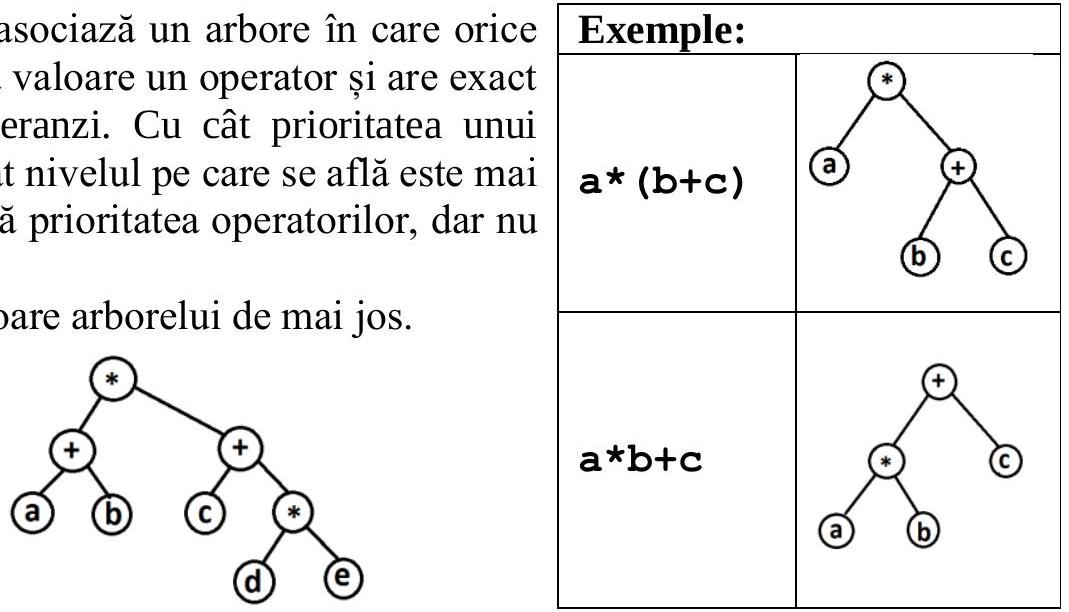
\includegraphics[max width=\textwidth, center]{2025_04_17_46e04c6acd873ea9558dg-022}
\\
a) a+b * c+d * e
\\
b) a+b *(c+d * e)
\\
c) (a+b) *(c+d * e)
\\
d) (a+b) * c+d * e
\\
e) a+b *(c+d) * e
\\
f) (a+b) * c+d * e
\\
3.11. Se consideră un tablou bidimensional $\mathbf{A}$ cu $\mathbf{n}$ linii și n coloane ( n - număr natural, $\mathrm{n}>\mathbf{1}$ ). Folosind rezolvarea optimă pentru fiecare caz, precizați care dintre problemele următoare se poate rezolva printr-un algoritm de complexitate minimă.
\\
a) Determinarea numărului de valori nule din $\mathbf{A}$
\\
b) Determinarea sumei elementelor de pe diagonala principală
\\
c) Determinarea rangului matricei $\mathbf{A}$
\\
d) Ordonarea crescătoare a elementelor de pe prima linie a tabloului prin apelarea celei mai eficiente metode de sortare
\\
e) Determinarea numărului de valori aflate sub diagonala principală
\\
f) Interschimbarea a două coloane ale tabloului
\\
3.12. Se consideră un graf orientat tare conex cu n noduri, numerotate $1,2,3, \ldots$ n. Pentru determinarea drumurilor de lungime minimă de la nodul 1 la celelalte noduri, s-a construit vectorul $\mathbf{t}$ în care $\mathrm{t}[\mathrm{i}]=\mathbf{k}$ dacă ( $\mathbf{k}, \mathbf{i}$ ) este ultimul arc al drumului minim de la nodul 1 la nodul i. Precizați instrucțiunea care poate înlocui punctele de suspensie astfel încât apelul drum ( $\mathrm{t}, \mathrm{n}$ ) să determine afișarea drumului de lungime minimă de la nodul 1 la nodul $n$.
\begin{verbatim}
Limbajul C++/ Limbajul C
    void drum(int t[ ], int i)
    {
        if (i!=1) .......
        cout<<i<<" ";
    }
Limbajul Pascal
type vector=array[1..100] of integer;
procedure drum(t:vector; i"integer);
begin
    if i<>1 then ........
    write(i, ' ' )
end;
\end{verbatim}
\\
a) drum(t, n);
\\
b) drum(t[i], i);
\\
c) drum(t, t[i]);
\\
d) drum(t, i);
\\
e) drum(t, 1);
\\
f) drum(t[i], t);
\\
3.13. \begin{center}
\begin{tabular}{|c|c|c|c|c|}
\hline
Vârful & $\mathbf{1}$ & $\mathbf{2}$ & $\mathbf{3}$ & $\mathbf{4}$ \\
\hline
Grad exterior & 2 & 0 & 2 & x \\
\hline
Grad interior & 0 & 2 & y & 1 \\
\hline
\end{tabular}
\end{center}
Precizați care din următoarele arce aparţine grafului orientat cu 4 vârfuri, având gradele din tabelul alăturat $(\mathbf{x}, \mathbf{y} \in \mathbf{N})$.\\
\\
a) $(1,2)$
\\
b) $(2,1)$
\\
c) $(2,3)$
\\
d) $(2,4)$
\\
e) $(3,1)$
\\
f) $(4,1)$
\\
3.14. Precizați care este numărul ciclurilor hamiltoniene disticte într-un graf complet cu 5 noduri. (Două cicluri sunt distincte dacă diferă prin cel puțin o muchie.)
\\
a) 5
\\
b) $4!/ 2$
\\
c) 4 !
\\
d) $4 * 4$ !
\\
e) 5 !
\\
f) $5^{4}$
\\
3.15. Precizați câte dintre afirmațiile următoare referitoare la grafuri neorientate sunt adevărate.
\begin{enumerate}
  \item Dacă gradul oricărui nod este un număr impar, atunci graful trebuie să aibă număr par de noduri.
  \item Un ciclu elementar este un caz particular de lanţ elementar.
  \item Numărul muchiilor grafului nu poate fi mai mic decât numărul nodurilor.
  \item Lungimea unui lanţ poate fi mai mare decât numărul de noduri al grafului.
  \item Numărul valorilor $\mathbf{1}$ din matricea de adiacență asociată este egal cu dublul numărului de muchii.
\end{enumerate}
\\
a) 0
\\
b) 1
\\
c) 2
\\
d) 3
\\
e) 4
\\
f) 5
\\

\section*{Varianta 4}

4.1. Variabila n reprezintă un număr natural cu exact două cifre. Precizați câte dintre expresiile următoare au valoarea 1 /true dacă și numai dacă cifrele lui $n$ au aceeași paritate.
Limbajul C++/ Limbajul C
\begin{verbatim}
1. (n/10-n%10)%2==0
2. n/10%2==n%2
3. n/10==n%10
4. (n/10+n%10*10) %2==n%2
5. n/2==n%2
\end{verbatim}
Limbajul Pascal
\begin{verbatim}
1. (n div 10 - n mod 10) mod 2 = 0
2. n div 10 mod 2 = n mod 2
3. n div 10=n mod 10
4. (n div 10 + n mod 10 *10) mod 2 = n mod 2
5. n div 2 = n mod 2
\end{verbatim}
\\
a) 0
\\
b) 1
\\
c) 2
\\
d) 3
\\
e) 4
\\
f) 5
\\
4.2. Pentru implementarea ecuației unei drepte de forma $\mathbf{a x + b y}+\mathbf{c}=0$ (unde $\mathbf{a}, \mathbf{b}, \mathbf{c} \in \mathrm{R}$ ), se definește structura:
\begin{verbatim}
Limbajul C++/ Limbajul C
typedef struct
    {float a, b, c;}dreapta;
\end{verbatim}
\begin{verbatim}
Limbajul Pascal
type dreapta=record
        a, b, c : real;
    end;
\end{verbatim}
Dacă d1 și d2 sunt două variabile de tipul dreapta, precizați care dintre următoarele expresii verifică dacă d1 și d2 sunt paralele.
\\
Limbajul C++/ Limbajul C
a) d1 \|\| d2
\\
b) d1.a==d2.a \&\& d1.b==d2.b
\\
c) a.d1/a.d2==b.d1/b.d2
\\
d) d1.a/d2.a==d1.b/d2.b
\\
e) d1.a==0 \&\& d2.a==0
\\
f) d1.a*d2.b-d1.b*d2.a==0
\\
Limbajul Pascal
a) d1 = d2
\\
b) (d1.a=d2.a) and (d1.b = d2.b)
\\
c) a.d1/a.d2 = b.d1/b.d2
\\
d) d1.a/d2.a=d1.b/d2.b
\\
e) (d1.a=0) and (d2.a=0)
\\
f) d1.a*d2.b-d1.b*d2.a=0
\\
4.3. Funcţia $\mathbf{f}$ primeşte ca parametri două valori reale şi returnează cea mai mare dintre cele două valori. Antetul funcției este:
(Limbajul C++/C) float f(float x, float y) ;
(Limbajul Pascal) function $f(x, y$ : real) :real;
Precizați care dintre următoarele expresii reprezintă suma celor mai mici două valori dintre numerele reale $\mathrm{a}, \mathrm{b}$ şi c .
\\
a) a+b+c-f(a, b)
\\
b) a+b+c-f(a, b)-f(b, c)
\\
c) a+2 * b+c-f(a, b)-f(b, c)
\\
d) a+b+c-f(a, b, c)
\\
e) a+b+c-f(a, f(c, b))
\\
f) a+b+c-f(f(a, b), f(b, a))
\\
4.4. Precizați care sunt valorile afișate în urma execuției următorului program.
\begin{verbatim}
Limbajul C++
#include<iostream>
using namespace std;
int a,b;
void f(int a, int &b)
{
    if (a>0)
        {
            a++; b--; f(b,a);
        }
    cout<<a<<" "<<b<<" ";
}
int main()
{ a=0; b=1;
    f(b,a);
    cout<<<a<<" "<<b;
}
\end{verbatim}
\begin{verbatim}
Limbajul C
#include<stdio.h>
int a,b;
void f(int a, int *b)
{
    if(a>0)
    {
        a++; (*b)--;
        f(*b,&a);
    }
    printf("%d %d",a,*b);
}
void main ( )
{
    a=0; b=1;
    f(b,&a) ;
    printf("%d %d",a,b);
}
\end{verbatim}
\begin{verbatim}
Limbajul Pascal
var a,b:integer;
procedure f(a:integer;
var b:integer);
begin
    if a>0 then
        begin
            a:=a+1; b:=b-1;
            f(b,a)
        end;
    write(a,' ',b,' ')
end;
begin
    a:=0; b:=1;
    f(b,a) ;
    write(a,' ',b,' ')
end.
\end{verbatim}
\\
a) -1 2 2 -1 -1 1
\\
b) 0 1 0 1
\\
c) Ciclare infinită
\\
d) -1 2 2 -1 0 1
\\
e) 0 2 0 -1 0 1
\\
f) -1 0 1 -1 1 1
\\
4.5. În secvența următoare variabilele n și m au ca valori numere naturale.
\begin{verbatim}
Limbajul C++/ Limbajul C
n=42015; m=0;
while(n>0)
    {
        m=m*100+n/10%10*10+n%10;
        n/=100;
    }
\end{verbatim}
\begin{verbatim}
Limbajul Pascal
n:=42015; m:=0;
while n>0 do
    begin
        m:=m*100+n div 10 mod 10*10+n mod 10;
        n:=n div 100;
    end;
\end{verbatim}
După rularea secvenței, valoarea variabilei $m$ este:
\\
a) 15024
\\
b) 15204
\\
c) 24051
\\
d) 51024
\\
e) 152004
\\
f) 152400
\\
4.6. Se consideră următorul program:
\begin{verbatim}
Limbajul C++
    #include<iostream>
    using namespace std;
    int main( )
    {
        int n, cn, x=0,p=1;
        cin>>n;
        cn=n;
        while(n)
        {
            if (n%10>x) x=n%10;
            n/=10;
        }
        x++;
        while(cn)
            {
            n=n+cn%10*p;
            p*=x;
            cn/=10;
            }
        cout<<n;
}
\end{verbatim}
\begin{verbatim}
Limbajul C
#include<stdio.h>
void main ( )
{
    int n, cn, x=0,p=1;
    scanf("%d", &n);
    cn=n;
    while(n)
        {
            if (n%10>x) x=n%10;
            n/=10;
        }
    x++;
    while(cn)
        {
            n=n+cn%10*p;
            p*=x;
            cn/=10;
        }
    printf("%d", n);
}
\end{verbatim}
\begin{verbatim}
var n,cn,x,p : longint;
begin
    readln(n);
cn:=n;
x:=0;
p:=1;
while n>0 do
begin
    if n mod 10>x then
        x:=n mod 10;
    n:=n div 10
end;
x:=x+1;
while cn>0 do
    begin
        n:=n+cn mod 10*p;
        p:=p*x;
        cn:=cn div 10
    end;
write(n)
end.
\end{verbatim}
Precizați care este cel mai mic număr natural format din 5 cifre distincte care poate fi citit ca dată de intrare astfel încât valoarea afișată să fie aceeași.
\\
a) 10000
\\
b) 10192
\\
c) 10234
\\
d) 10239
\\
e) 10923
\\
f) 12345
\\
4.7. Tabloul bidimensional b(cu liniile și coloanele numerotate de la 1 la $\mathbf{n}$ ) se obține din tabloul bidimensional a prin rotire cu $90^{\circ}$ spre dreapta.
De exemplu, dacă a este: (123456789) se obține tabloul bidimensional b:(741852963)
Pentru obținerea unei transformări corecte, secvența:
\begin{verbatim}
Limbajul C++/ Limbajul C
for (i=1; i<=n ; i++)
    for (j=1; j<=n; j++) ......;
Limbajul Pascal
for i:=1 to n do
    for i:=1 to n do .......;
\end{verbatim}
trebuie completată cu atribuirea:
\\
Limbajul C++/ Limbajul C
a) b[i][j]=a[j][i]
\\
b) b[i][j]=a[j][n-i+1]
\\
c) b[i][j]=a[n-j+1][n-i+1]
\\
d) b[i][j]=a[n-i+1][n-j+1]
\\
e) b[i][j]=a[n-j+1][i]
\\
f) b[i][j]=a[n-i+1][j]
\\
Limbajul Pascal
a) b[i][j]:=a[j][i]
\\
b) b[i,j]:=a[j,n-i+1]
\\
c) b[i, j]:=a[n-j+1, n-i+1]
\\
d) b[i, j]:=a[n-i+1, n-j+1]
\\
e) b[i, j]:=a[n-j+1, i]
\\
f) b[i, j]:=a[n-i+1, j]
\\
4.8. Variabila $\mathbf{x}$ este de tip întreg și reprezintă o cifră nenulă. Precizați care dintre expresiile - următoare este echivalentă cu expresia:
\begin{verbatim}
(Limbajul C++/C) x == 7 || x == 5
(Limbajul Pascal) (x=7) or (x=5)
\end{verbatim}    
\\
Limbajul C++/ Limbajul C
a) 35 \% x==0
\\
b) x!=7 \&\& x!=5
\\
c) x>4 \&\&!(x \% 2==0 \|\| x \% 3==0)
\\
d) x \% 2!=0 \&\& x \% 3!=0
\\
e) ! (x!=7 \|\| 1 x!=5)
\\
f) x>4 \&\&!(x \% 2==0 \&\& x \% 3==0)
\\
Limbajul Pascal
a) 35 mod x=0
\\
b) ( x<>7 ) and ( x<>5 )
\\
c) (x>4) and not((x mod 2=0) or (x mod 3=0))
\\
d) ( x mod 2<>0 ) and ( x moc 3<>0 )
\\
e) not((x<>7) or (x<>5))
\\
f) (x>4) and not((x mod 2=0) and (x mod 3=0)
\\
4.9. Tabloul unidimensional a conține n numere naturale, ordonate crescător. Se cere afișarea mesajului DA dacă în a există două elemente a căror diferență este egală cu s (număr natural) sau a mesajului NU, în caz contrar. Precizați condiția ce trebuie utilizată în locul punctelor de suspensie astfel încât secvența următoare să rezolve corect problema dată.
\begin{verbatim}
Limbajul C++/C
i = 1; j = 2;
while ( ....... )
    {
        if (a[j]-a[i]<s) j++;
        else i++;
    }
if (j <= n) cout<<"DA"; |
printf("DA");
else cout<<"NU"; | printf("DA");
\end{verbatim}
\begin{verbatim}
Limbajul Pascal
i:= 1; j:= 2;
while ....... do
    begin
        if a[j]-a[i]<s then inc(j)
        else inc(i);
    end;
if $j<=n$ then write('DA')
else write('NU');
\end{verbatim}
\\
Limbajul C++/C
a) j<n
\\
b) j<=n \& & a[j]-a[i]!=s
\\
c) j<=n \&\& a[j]-a[i]==s
\\
d) a[j]-a[i]!=s
\\
e) i<=j
\\
f) i<=n \&\& a[j]-a[i]==s
\\
Limbajul Pascal
a) j<n
\\
b) (j<=n) and (a[j]-a[i]<>s)
\\
c) (j<=n) and (a[j]-a[i]=s)
\\
d) a[j]-a[i]<>s
\\
e) i<=j
\\
f) (i<=n) and (a[j]-a[i]=s)
\\
4.10. Precizați care este rolul următorului subprogram.
\begin{verbatim}
Limbajul C++/ Limbajul C
void f(char s[],char t[],int k)
{
    char aux[255];
    strcpy(aux,s+k);
    s[k]=0;
    strcat(s,t);
    strcat(s,aux);
}
\end{verbatim}
\begin{verbatim}
Limbajul Pascal
procedure f(var s:string;t:string;
k:byte);
var aux:string;
begin
    aux:=copy(s,k,255);
    delete(s,k,255);
    s:=concat(s,t);
    s:=concat (s,aux);
end;
\end{verbatim}
\\
a) Șterge ultimele $\mathbf{k}$ caractere ale lui $\mathbf{s}$ și concatenează rezultatul cu șirul $\mathbf{t}$
\\
b) Concatenează șirul s cu rezultatul concatenării șirurilor s și $t$
\\
c) Inserează șirul sîn șirul $t$, începând cu poziția $\mathbf{k}$
\\
d) Concatenează șirurile $\mathbf{s}$ și $\mathbf{t}$, obținând un șir de lungime $\mathbf{k}$
\\
e) Înlocuiește primele $\mathbf{k}$ caractere din $\mathbf{s}$ cu primele $\mathbf{k}$ caractere din $\mathbf{t}$
\\
f) Inserează șirul $\mathbf{t}$ în șirul $\mathbf{s}$, începând cu poziția $\mathbf{k}$
\\
4.11. Se consideră un graf orientat cu 6 noduri, numerotate $1,2, \ldots, 6$. Arcele grafului sunt de forma $(\mathbf{x}, \mathbf{2 *} \mathbf{x})$ pentru orice $\mathbf{x} \in\{1,2,3\}$ și de forma $(\mathbf{x}, \mathbf{x}-\mathbf{1})$ pentru orice $\mathbf{x} \in\{2,3,4,5,6\}$. Care este numărul minim de arce ce trebuie adăugate astfel încât graful să fie tare conex?
\\
a) 0
\\
b) 1
\\
c) 2
\\
d) 3
\\
e) 4
\\
f) 5
\\
4.12. Precizați care dintre tablourile următoare poate reprezenta vectorul gradelor unui graf neorientat conex.
\\
a) (3,2,1,5,1,1)
\\
b) (5,1,6,4,5,3)
\\
c) (1,1,1,1,2,2)
\\
d) (1,1,1,1,1,6)
\\
e) (2,1,3,1,0,1)
\\
f) (1,3,5,2,1,2)
\\
4.13. Dacă un graf neorientat conex are $\mathbf{n}$ vârfuri și $3 n+2$ muchii, precizați care este valoarea minimă pentru n .
\\
a) 16
\\
b) 8
\\
c) 4
\\
d) 2
\\
e) 1
\\
f) 0
\\
4.14. Pentru un număr natural nenul $n$, se construiește un arbore cu rădăcină astfel: rădăcina este numerotată n și orice nod care este numerotat cu o valoare $\mathbf{x}>1$ are ca fii nodurile numerotate cu divizorii săi, mai puțin numărul însuși. Toate frunzele arborelui sunt numerotate cu 1. Precizați câte dintre numerele naturale din intervalul $[10,20]$ pot fi alese ca rădăcină, astfel încât arborele asociat să aibă un număr maxim de frunze.
\\
a) 1
\\
b) 2
\\
c) 3
\\
d) 4
\\
e) 5
\\
f) 6
\\
4.15. Un pulover norvegian este frumos dacă pentru a-l tricota se folosesc cel puțin 2 și cel mult 4 culori de lână. Precizați câte modalități de combinare a culorilor există pentru a tricota un pulover norvegian frumos, având la dispoziție 5 ghemuri de lână de culori diferite.
\\
a) 5
\\
b) 12
\\
c) 24
\\
d) 25
\\
e) 48
\\
f) 125
\\

\section*{Varianta 5}

5.1. Precizați care dintre următoarele expresii are valoarea $\mathbf{1} /$ true dacă şi numai dacă numărul natural nenul memorat în variabila $\mathbf{x}$ nu este divizibil cu 6 .
\\
Limbajul C++/ Limbajul C
a) x / 6==0
\\
b) x==6
\\
c) x \%==0
\\
d) x / 6>0
\\
e) x \% 2+x \% 3>0
\\
f) x>6
\\
Limbajul Pascal
a) x div 6=0
\\
b) x=6
\\
c) x mod 6=0
\\
d) x / 6>0
\\
e) x mod 2+x mod 3>0
\\
f) x>6
\\
5.2. Precizațic care dintre următoarele instrucțiuni este corectă dacă variabilele $\mathbf{x}, \mathbf{y}$ și $\mathbf{z}$ au declarările de mai jos:
\begin{verbatim}
Limbajul C++/ Limbajul C
float x;
int y, z;
Limbajul Pascal
x : real;
y,z: integer;
\end{verbatim}
\\
Limbajul C++/ Limbajul C
a) x = x *y\%z;
\\
b) x=z \% y* x;
\\
c) x=x\%y*z;
\\
d) x=x* z \% x;
\\
e) x=x \% z;
\\
f) y=z \% x;
\\
Limbajul Pascal
a) x:=x*y mod z;
\\
b) x:=z mod y* x;
\\
c) x:=xmod y*z;
\\
d) x:=x*z mod \x;
\\
e) x:=x mod z;
\\
f) y:=z mod x ;
\\
5.3. Precizați ce valoare se va afişa pe ecran în urma executării secvenței de program următoare, ştiind că s este o variabilă care memorează un şir de caractere, iar i este o variabilă de tip întreg.
\begin{verbatim}
Limbajul C++/ Limbajul C
strcpy(s,"admitere");
for(i=0;i<strlen(s);i++)
    if(strchr("politehnica",s[i]))
        strcpy(s+i,s+i+1);
cout<<s; | printf("%s",s);
\end{verbatim}
\begin{verbatim}
Limbajul Pascal
s:='admitere';
for i:=1 to length(s) do
    if pos(s[i],'politehnica')>0 then
        delete(s,i,1);
write(s);
\end{verbatim}
\\
a) dmt
\\
b) dm
\\
c) dmtr
\\
d) dmr
\\
e) mt
\\
f) mrt
\\
5.4. Precizați care dintre următoarele afirmații este adevărată pentru orice graf neorientat $\mathbf{G}$ format din 100 de noduri și 100 de muchii.
\\
a) Graful G nu este conex
\\
b) Graful G este conex
\\
c) Graful G este complet
\\
d) Graful G conține cel puțin un ciclu
\\
e) Graful G nu are noduri izolate
\\
f) Graful G conține un lanț elementar de lungime 100
\\
5.5. Pentru reprezentarea unui graf orientat $\mathbf{G}$ se utilizează matricea de adiacență. Precizați care este suma elementelor din această matrice dacă graful are 20 de noduri și 30 de arce.
\\
a) 60
\\
b) 50
\\
c) 40
\\
d) 30
\\
e) 20
\\
f) 10
\\
5.6. Precizați care este lungimea maximă a unui lanț simplu (lanț în care fiecare muchie apare o singură dată) într-un arbore cu 10 noduri în care fiecare nod are gradul un număr impar.
\\
a) 9
\\
b) 8
\\
c) 7
\\
d) 6
\\
e) 5
\\
f) 4
\\
5.7. Tabloul unidimensional $\mathbf{v}$ conține $\mathbf{n}$ numere întregi numerotate de la 1 la $\mathbf{n}$. Precizați care dintre următoarele secvențe determină înlocuirea primului element din tabloul unidimensional $\mathbf{v} \mathbf{c u}$ cea mai mică valoare care apare în acesta.
\\
Limbajul C++/ Limbajul C
a) \begin{verbatim}
 for (i=1; i<n; i++)
    if(v[i]>v[i+1])
    \{
        $a=v[i]$;
        v[i]=v[i+1];
        v[i+1]=a;
    \}
\end{verbatim}
\\
b) \begin{verbatim}
for(i=n-1; i>=1; i--)
    if (v[i]>v[i+1])
    {
        a=v[i];
        v[i]=v[i+1];
        v[i+1]=a ;
    }
\end{verbatim}
\\
c) \begin{verbatim}
for(i=n-1; i>=1; i--)
    if(v[i]<v[i+1])
    {
        a=v[i];
        v[i]=v[i+1];
        v[i+1]=a;
    }
\end{verbatim}
\\
d) \begin{verbatim} 
for (i=1; i<=n-1; i++)
    if(v[i]<v[i+1])
    {
        a=v[i];
        v[i]=v[i+1];
        v[i+1]=a;
    }
\end{verbatim}
\\
e) \begin{verbatim}
for (i=n-1; i>=1; i--)
    if (v[i]<v[i+1])
    {
        a=v[i+1];
        v[i]=v[i+1];
        v[i+1]=a ;
    }
\end{verbatim}
\\
f) \begin{verbatim}
for (i=1; i<=n-1; i++)
    if(v[i]<v[i+1])
    {
        a=v[i+1];
        v[i]=v[i+1];
        v[i+1]=a;
    }
\end{verbatim}
\\
Limbajul Pascal
a) \begin{verbatim}
for $i:=1$ to $n-1$ do
    if v[i]>v[i+1] then
        begin
            a:=v[i];
            v[i]:=v[i+1];
            v[i+1]:=a;
        end;
\end{verbatim}
\\
b) \begin{verbatim}
for i:=n-1 downto 1 do
    if v[i]>v[i+1] then
        begin
            a:=v[i];
            v[i]:=v[i+1];
            v[i+1]:=a;
        end;
\end{verbatim}
\\
c) \begin{verbatim}
for i:=n-1 downto 1 do
    if v[i]<v[i+1] then
        begin
            a:=v[i];
            v[i]:=v[i+1];
            v[i+1]:=a;
        end;
\end{verbatim}
\\
d) \begin{verbatim}
for i:=1 to n-1 do
    if v[i]<v[i+1] then
        begin
            a:=v[i];
            v[i]:=v[i+1];
            v[i+1]:=a;
        end;
\end{verbatim}
\\
e) \begin{verbatim}
for i:=n-1 downto 1 do
    if v[i]<v[i+1] then
        begin
            a:=v[i+1];
            v[i]:=v[i+1];
            v[i+1]:=a;
        end;
\end{verbatim}
\\
f) \begin{verbatim}
for i:=1 to n-1 do
    if v[i]<v[i+1] then
        begin
            a:=v[i+1];
            v[i]:=v[i+1]'
            v[i+1]:=a;
        end;
\end{verbatim}
\\
5.8. Precizați pentru care dintre următoarele tablouri unidimensionale se poate aplica algoritmul căutării binare cu scopul de a găsi în mod eficient, dacă există, numere care au cifra unităților egală cu o valoare x , dată.
\\
a) (1,21,13,23,33,17,27)
\\
b) (1,13,17,21,23,27,33)
\\
c) (1,13,33,17,21,23,27)
\\
d) (33,27,23,21,17,13,1)
\\
e) (1,13,33,21,23,27,17)
\\
f) (33,27,23,21,13,1,17)
\\
5.9. În secvenţa de mai jos, variabila a memorează un tablou bidimensional cu 4 linii şi 4 coloane, numerotate de la 1 la 4, cu elementele întregi. Variabila s este întreagă, iar i este de tip întreg. Precizați care dintre instrucţiunile de mai jos poate înlocui punctele de suspensie, astfel încât secvența să determine memorarea în variabila s, a valorii sumei elementelor aflate pe prima și ultima coloană ale matricei.
\begin{verbatim}
Limbajul C++/ Limbajul C
s=0;
for (i=1;i<=4;i++)....
Limbajul Pascal
s:=0;
for i:=1 to 4 do .....
\end{verbatim}
\\
Limbajul C++/ Limbajul C
a) s=s+a[4][i]+a[i][4];
\\
b) s=s+a[4-i][4]+a[i][1];
\\
c) s=s+a[i][1]+a[i][4];
\\
d) s=s+a[i][i]+a[1][i] ;
\\
e) s=s+a[1][i]+a[4][i];
\\
f) s=s+a[i][i]+a[5-i][i];
\\
Limbajul Pascal
a) s:=s+a[4, i]+a[i, 4];
\\
b) s:=s+a[4-i, 4]+a[i, 1];
\\
c) s:=s+a[i, 1]+a[i, 4];
\\
d) s:=s+a[i, i]+a[1, i];
\\
e) s:=s+a[1, i]+a[4, i];
\\
f) s:=s+a[i, i]+a[5-i, i];
\\
5.10. Utilizând metoda backtracking se generează toate anagramele cuvântului avion. Precizați câte anagrame încep și se termină cu câte o consoană.
\\
a) 6
\\
b) 12
\\
c) 20
\\
d) 36
\\
e) 38
\\
f) 40
\\
5.11. Subprogramul $\mathbf{f}$ are definiţia următoare. Dacă variabilele a și b sunt de tip întreg și memorează valorile 3 respectiv 5 , precizați care vor fi valorile pe care le memorează variabilele a și b după apelul:
\begin{verbatim}
f(a,b); (Limbajul Pascal/C++)
f(a, &b); (Limbajul C)
\end{verbatim}
\begin{verbatim}
Limbajul C++
void f(int x,int &y)
    {int aux;
        aux=x; x=y;
        y=aux;
    }
Limbajul C
void f(int x,int *y)
    {int aux;
        aux=x; x=*y;
        *y=aux;
    }
Limbajul Pascal
    procedure f(x:integer;var y:integer);
        var aux:integer;
    begin
            aux:=x; x:=y; y:=aux;
    end;
\end{verbatim}
\\
a) 3 și 3
\\
b) 4 și 3
\\
c) 5 și 5
\\
d) 3 și 5
\\
e) 3 și 4
\\
f) 5 și 3
\\
5.12. Considerăm declararea următoare, folosită pentru a memora numărătorul și numitorul unei fracții. Precizați care dintre instrucțiunile de mai jos este corectă.
\begin{verbatim}
Limbajul C++/ Limbajul C
typedef struct
    { int a, b; }fractie;
fractie m,n;
\end{verbatim}
\begin{verbatim}
Limbajul Pascal
type fractie=record
        a,b:integer;
    end;
var m,n:fractie;
\end{verbatim}
\\
Limbajul C++/ Limbajul C
a) m=n;
\\
b) if (m>n) m++;
\\
c) if (m==n) m--;
\\
d) if (m<=n) m=n;
\\
e) if (m!=n) m--;
\\
f) if (m>n) m=n;
\\
Limbajul Pascal
a)m:=n;
\\
b) if (m>n) then m:=m+1;
\\
c) if (m=n) then m:=m-1;
\\
d) if (m<=n) then m:=n;
\\
e) if (m<>n) then m:=m-1;
\\
f) if (m>n) then m:=n;
\\
5.13. Precizați care este numărul de grafuri orientate distincte formate din 3 noduri și $\mathbf{4}$ arce. Două grafuri sunt distincte dacă au matricea de adiacență diferită.
\\
a) 32
\\
b) 30
\\
c) 20
\\
d) 16
\\
e) 15
\\
f) 9
\\
5.14. Precizați care este instrucţiunea prin care variabilei $\mathbf{y}$ i se atribuie numărul obținut prin inversarea ordinii cifrelor numărului natural format din exact 2 cifre, memorat în variabila întreagă $\mathbf{x}$.
\\
Limbajul C++/ Limbajul C
a) y=x/10*10+x\%100;
\\
b)  y=x\%10+x/10;
\\
c)  y=x/10*10+x\%10;
\\ 
d)  y=x\%100/10;
\\
e)  y=x*10\%100+x/10;
\\ 
f)  y=x\%10/10;
\\
Limbajul Pascal
a)  y:=x div 10*10+x mod 100;
\\
b)  y:=x mod 10 +x div 10;
\\
c)  y:=x div 10*10+x mod 10;
\\
d)  y:=x mod 100 div 10;
\\
e)  y:=x*10 mod 100+x div 10;
\\
f)  y:=x mod 10 div 10;
\\
5.15. Fie $\mathbf{G}$ un graf neorientat complet cu 100 de noduri. Precizați care dintre următoarele afirmații este adevarată:
\\
a) În graful G există un lanț elementar de lungime 100
\\
b) Graful g este un graf hamiltonian
\\
c) Graful g este un graf eulerian
\\
d) Graful g nu este conex
\\
e) Graful g are 900 de muchii
\\
f) Graful G are două componente conexe
\\

\section*{Varianta 6}

6.1. Precizați care este valoarea maximă pe care o poate avea expresia de mai jos în care $\mathbf{x}$ este $o$ variabilă de tip întreg.
\begin{verbatim}
Limbajul C++/ Limbajul C
2 * x % 10 * 2 % 10
Limbajul Pascal
2 * x mod 10 * 2 mod 10
\end{verbatim}
\\
a) 9
\\
b) 8
\\
c) 7
\\
d) 0
\\
e) 10
\\
f) 20
\\
6.2. Variabilele întregi a şi b memorează câte un număr natural nenul. Precizați care dintre următoarele expresii are valoarea true/1 dacă și numai dacă valorile memorate de a și b au aceeași paritate.
\\
Limbajul C++/ Limbajul C
a) a==b
\\
b) a \% 2==0 \&\& b \% 2==0
\\
c) (a+b) \% 2==0
\\
d) a * b \% 2==0
\\
e) a \% b==2
\\
f) a / b==2
\\
Limbajul Pascal
a) a=b
\\
b) (a mod 2=0) and (b mod 2=0)
\\ 
c) (a+b) mod 2 = 0
\\
d) a*b mod 2=0
\\
e) a mod b=2
\\
f) a div b = 2
\\
6.3. Precizați ce se afişează în urma executării secvenţei de program de mai jos, dacă variabilele a și b pot memora câte un şir de cel mult 100 de caractere.
\begin{verbatim}
Limbajul C++/ Limbajul C
strcpy (a,"matematica");
strcpy (b, strstr(a,"ema") +2) ;
strcat(b,strchr(a,a[3])+1);
cout<<b; | printf("\%s",b);
\end{verbatim}
\begin{verbatim}
Limbajul Pascal
a:='matematica';
b:=copy(a,pos('ema',a)+2,length(a));
b:=b+copy (a,pos (a [4],a) +1, length (a));
write(b);
\end{verbatim}
\\
a) aticamatica
\\
b) maticamatica
\\
c) maticaatica
\\
d) matica
\\
e) matematica
\\
f) atica
\\
6.4. Fie un graf neorientat complet cu 10 noduri. Precizați care este numărul minim de muchii care trebuie eliminate astfel încât graful parțial obținut să nu fie conex.
\\
a) 1
\\
b) 9
\\
c) 8
\\
d) 7
\\
e) 6
\\
f) 5
\\
6.5. Precizați care dintre următoarele ș̦iruri de grade corespund unui graf neorientat cu 6 noduri.
\\
a) (1,2,3,4,5,6)
\\
b) (0,1,2,3,4,5)
\\
c) (0,1,0,1,0,1)
\\
d) (1,2,2,1,2,2)
\\
e) (1,1,1,1,1,2)
\\
f) (1,2,2,1,1,2)
\\
6.6. Precizați care este numărul maxim de frunze ce apar într-un arbore cu 17 de noduri, dacă fiecare nod are gradul mai mic sau egal cu 4.
\\
a) 11
\\
b) 12
\\
c) 13
\\
d) 14
\\
e) 15
\\
f) 16
\\
6.7. Graful orientat G are 10 noduri și 12 arce. Precizați care este cel mai mare grad exterior al unui nod din acest graf, dacă G este tare conex.
\\
a) 12
\\
b) 3
\\
c) 10
\\
d) 4
\\
e) 5
\\
f) 6
\\
6.8. Se consideră un tablou bidimensional a cu n linii şi n coloane, numerotate de la 1 la $n, \mathrm{cu}$ elemente numere întregi. Precizați ce reprezintă valoarea variabilei întregi $\mathbf{x}$, după executarea secvenței de program de mai jos.
\begin{verbatim}
Limbajul C++/ Limbajul C
x=0;
for(i=1;i<=n;i++) x=x+a[i][n-i+1];
Limbajul Pascal
x:=0; 
for i:=1 to n do x:=x+a[i,n-i+1];
\end{verbatim}
\\
a) suma elementelor de pe diagonala principală a tabloului a
\\
b) suma elementelor de pe diagonala secundară a tabloului a
\\
c) suma elementelor tabloului a
\\
d) suma elementelor situate pe ultima coloană a tabloului a
\\
e) suma elementelor situate pe prima coloană a tabloului a
\\
f) suma elementelor situate pe ultima linie a tabloului a
\\
6.9. Se consideră secvența alăturată în care A este un tablou bidimensional cu cinci linii şi cinci coloane, numerotate de la 1 la 5, iar $\mathbf{x}$ și i sunt variabile de tip întreg. Ştiind că orice element al tabloului este inițial egal cu numărul de ordine al liniei pe care se află, precizaţi care este valoarea variabilei $\mathbf{x}$ după executarea secvenței de mai jos?
\begin{verbatim}
Limbajul C++/ Limbajul C
x=0;
for(i=1;i<=5;i++)
    if(i%2==0) x=x+A[i-1][i];
\end{verbatim}
\begin{verbatim}
Limbajul Pascal
x:=0;
for i:=1 to 5 do
    if ( i mod 2 = 0) then x:=x+A[i-1,i];
\end{verbatim}
\\
a) 25
\\
b) 4
\\
c) 15
\\
d) 5
\\
e) 30
\\
f) 3
\\
6.10. Problema generării tuturor numerelor formate din exact trei cifre nenule, cu toate cifrele distincte două câte două, este similară cu generarea:
\\
a) aranjamentelor
\\
b) permutărilor
\\
c) elementelor produsului cartezian
\\
d) tuturor submultimilor unei mulțimi
\\
e) combinărilor
\\
f) partițiilor unei mulțimi
\\
6.11. O delegație formată din patru elevi ai unei grupe trebuie să participe la o conferință. Știind că în grupă sunt $\mathbf{9}$ elevi, dintre care cinci sunt fete, precizați care este numărul posibilităț̦ilor de a forma delegația care va participa la conferință, dacă aceasta trebuie să fie alcătuită din doi băieți și două fete.
\\
a) 20
\\
b) 45
\\
c) 180
\\
d) 60
\\
e) 90
\\
f) 120
\\
6.12. Fie un șir format din 10000 de numere naturale, fiecare având cel mult 9 cifre. Precizați care dintre următorii algoritmi efectuează un număr minim de pași.
\\
a) ordonarea crescătoare a elementelor din șir
\\
b) numărarea elementelor prime din șir
\\
c) determinarea elementului maxim din șir
\\
d) verificarea unicității tuturor elementelor din șir
\\
e) generarea tuturor permutărilor elementelor din șir
\\
f) suma elementelor care apar de exact două ori în șir
\\
6.13. În declararea alăturată, câmpurile $\mathbf{x}$ şi $\mathbf{y}$ ale înregistrării pot memora coordonatele carteziene ale unui punct din planul $x O y$. Precizați care dintre următoarele expresii are valoarea true/1 dacă şi numai dacă punctul P este situat în cadranul I sau III, dar nu și pe axe.
\begin{verbatim}
Limbajul C++/ Limbajul C
typedef struct
    {
        float x,y;
    } punct;
punct p;
\end{verbatim}
\begin{verbatim}
Limbajul Pascal
type punct=record
    x,y:real;
    end;
var p:punct;
\end{verbatim}
\\
a) p.x*p.y>0
\\
b) p.x>p.y
\\
c) p.x*p.y>=0
\\
d) x.p*y.p>0
\\
e) x.p*y.p>0
\\
f) p.x+p.y>=0
\\
14 Precizați care este suma maximă a elementelor care apar într-un tablou unidimensional cu legături „de tip tată", asociat unui arbore cu rădăcină format din 10 noduri, etichetate cu numere de la 1 la 10 .
\\
a) 100
\\
b) 90
\\
c) 81
\\
d) 45
\\
e) 80
\\
f) 60
\\
6.15. Subprogramul f are definiţia de mai jos. Dacă variabila a este de tip întreg și memorează valorarea 3, precizați care va fi valorea pe care o memorează aceeași variabilă a, după apelul $\mathrm{f}(\mathrm{a}, \mathrm{a})$; (limbajul Pascal/C++), respectiv $\mathrm{f}(\varepsilon a, \& a)$; (în limbajul C).
\begin{verbatim}
Limbajul C++
void f(int &x,int &y)
{
    x=1;
    x=x+y;
}
Limbajul C
void f(int *x, int *y) 
{ 
   *x=1; 
   *x=*x+*y; 
} 
Limbajul Pascal
procedure f(var x,y: integer);
begin
x:=1;
x:=x+y;
end;
\end{verbatim}
\\
a) 1
\\
b) 2
\\
c) 3
\\
d) 4
\\
e) 5
\\
f) 6
\\

\section*{Varianta 7}

\begin{enumerate}
  \item Indicaţi care dintre expresiile $\mathrm{C}++/ \mathrm{C} /$ Pascal de mai jos are valoarea true/1 dacă și numai dacă numărul memorat în variabila întreagă x aparţine reuniunii de intervale:
\end{enumerate}

\begin{verbatim}
$[-4,-1] \cup[1,4] \cup[10, \infty)$.
Limbajul C++/ Limbajul C
a) $x>=-4$ \&\& $x<=-1 \quad \& \& \quad x>=1 \quad \& \& \quad x<=4 \quad \& \& \quad x>=10$
b) ! ( $x<-4$ || $x>-1$ ) || ! ( $x<1$ || $x>4$ ) || ! $(x<10)$
c) $x>=-4$ || $x<=-1$ || $x>=1$ || $x<=4$ || $x>=10$
d) ! $(x<-4 \& \& \quad x>4 \& \& x>-1 \quad| | x<1 \& \& x>=10)$
e) ! $(x<-4| | x>-1) \& \&!(x<1| | x>4) \quad| |!(x<10)$
f) ! ( $x<-4$ || $x>-1$ ) \&\& ! $(x<1| | x>4) \& \&!(x<10)$
Limbajul Pascal
a) $(x>=-4)$ and $(x<=-1)$ and $(x>=1)$ and $(x<=4)$ and ( $x>=10)$
b) not(( $x<-4$ ) or ( $x>-1)$ ) or not( $(x<1)$ or ( $x>4)$ ) or not $(x<10)$
c) ( $x>=-4$ ) or ( $x<=-1$ ) or ( $x>=1$ ) or ( $x<=4$ ) or ( $x>=10$ )
d) $\operatorname{not}((x<-4)$ and $(x>4)$ and ( $x>-1)$ or ( $x<1$ ) and ( $x>=10)$ )
e) $\operatorname{not}((x<-4)$ or $(x>-1))$ and $\operatorname{not}((x<1)$ or $(x>4))$ or $\operatorname{not}(x<10)$
f) $\operatorname{not}((x<-4)$ or $(x>-1))$ and $\operatorname{not}((x<1)$ or $(x>4))$ and $\operatorname{not}(x<10)$
\end{verbatim}

\begin{enumerate}
  \setcounter{enumi}{1}
  \item Indicați expresia $\mathrm{C}++/ \mathrm{C} /$ Pascal care are valoarea true /1:
\end{enumerate}

Limbajul C++/ Limbajul C\\
a) floor (5) $+1==\operatorname{ceil}(5)$\\
b) floor(5.49) $==$ ceil(5.49)\\
c) floor(5.19) $==$ floor(5.91)\\
d) floor(5.91) $==$ ceil(5.19)\\
e) floor(sqrt(8))==ceil(sqrt(8))\\
f) $\operatorname{sqrt}(4)==\operatorname{pow}(4,2)$

Limbajul Pascal\\
a) trunc (5) +1 $=$ round (5)\\
b) trunc(5.19) $=$ round (5.91)\\
c) trunc(5.19) $=$ trunc(5.91)\\
d) round(5.91) $=$ round (5.19)\\
e) round (sqrt(8)) =trunc (sqrt (8))\\
f) $\operatorname{sqrt}(4)=\operatorname{sqr}(4)$\\
3. Se consideră două tablouri unidimensionale $A$ şi $B$. Știind că $A=(7,10,12,18,20)$, iar în urma interclasării tablourilor A şi B, în ordine descrescătoare, se obține tabloul cu elementele $(46,20,18,17,12,10,10,7,4,3)$. Atunci tabloul B poate fi:\\
a) $(3,4,17,46)$\\
b) $(3,4,10,46)$\\
c) $(3,4,10,17)$\\
d) $(3,4,10,17,46)$\\
e) $(46,17,4,3)$\\
f) $(46,10,4,3)$\\
4. Pentru a verifica dacă într-un tablou unidimensional având elementele $(3,4,7,10,12,17,18,20,46)$ există elementul cu valoarea $\mathbf{x}=17$, se aplică metoda căutării binare. Ştiind că numerotarea elementelor, în tablou, se realizează începând cu poziţia 0 , care este numărul minim de elemente ale tabloului care trebuie verificate pentru a găsi elementul căutat?\\
a) 6\\
b) 2\\
C) 9\\
d) 5\\
e) 3\\
f) 1\\
5. Variabila $\mathbf{x}$ este de tip real și poate memora un număr real din intervalul $[32,48]$. Numărul valorilor distincte pe care le poate avea expresia următoare este:

\begin{verbatim}
Limbajul C++/C
floor(sqrt(x+1))
\end{verbatim}

Limbajul Pascal

\begin{verbatim}
trunc(sqrt(x+1))
\end{verbatim}

a) 17\\
b) 1\\
c) 0\\
d) 2\\
e) 4\\
f) 3\\
6. Un grup format din şase prieteni (Andrei, Bogdan, Claudiu, Daniel, Emil, Florin) doreşte să participe la o competiţie de baschet pentru echipe formate din câte trei jucători. Ştiind că echipa Andrei, Bogdan, Claudiu este identică cu echipa Bogdan, Claudiu, Andrei, precizați care este numărul de echipe care se pot forma cu cei şase prieteni.\\
a) 2\\
b) 720\\
c) 120\\
d) 20\\
e) 6\\
f) 3\\
7. Fie subprogramul recursiv următor:

\begin{verbatim}
Limbajul C++
void ex(char c)
{ if (c>'a')
            ex(c-1);
        cout<< C;
    if (c>'a')
            ex(c-1);
}
\end{verbatim}

\begin{verbatim}
Limbajul C
void ex(char c)
{ if (c>'a')
            ex(c-1);
        printf("%c", c);
    if (c>'a')
            ex(c-1);
}
\end{verbatim}

\begin{verbatim}
Limbajul Pascal
procedure ex(c:char)
begin
    if (c>'a') then
ex(pred(c));
        write(c);
        if (c>'a') then
ex(pred(c));
end;
\end{verbatim}

Indicați numărul de autoapeluri ale subprogramului dacă se apelează ex (' c' ) :\\
a) 0\\
b) 1\\
c) 7\\
d) 3\\
e) 6\\
f) 5\\
8. Într-un program $\mathrm{C}++/ \mathrm{C} /$ Pascal în care a este o variabilă de tip întreg, se citesc datele din fişierul "admitere.dat" utilizând următoarea instruç̧iune:

Limbajul C++\\
Limbajul C\\
Limbajul Pascal\\
f>>a;

\begin{verbatim}
fscanf(f, "%d", &a);
\end{verbatim}

Precizaţi care este forma corectă a instrucţiunii ce are ca efect închiderea fişierului utilizat:\\
Limbajul C++\\
Limbajul C\\
Limbajul Pascal

\begin{verbatim}
a) close(f);
b) close (admitere) ;
c) admitere.close () ;
d) close.admitere;
e) close.f;
f) f.close();
\end{verbatim}

\begin{verbatim}
a) fclose (admitere) ;
b) close (admitere) ;
c) close (f) ;
d) admitere (close) ;
e) close.f
f) fclose (f) ;
\end{verbatim}

a) f.close();\\
b) admitere.close();\\
c) close(admitere);\\
d) admitere (close);\\
e) close.f;\\
f) close(f);\\
9. Se consideră următoarea secvență de instrucțiuni:

\begin{verbatim}
Limbajul C++ Limbajul C
char cif; int cifra; char cif; int cifra;
cin>>cif; scanf("%c", &cif);
cifra = cif - '0'; cifra = cif-'0';
cout<< cifra; printf ("%d", cifra);
\end{verbatim}

\begin{verbatim}
Limbajul Pascal
var cif: char;
    cifra: integer;
begin
    read(cif);
cifra:=ord(cif) -ord('0');
    write (cifra);
end.
\end{verbatim}

Precizați ce se afişează după executarea acestei secvenţe dacă, în urma operaţiei de citire, variabila cif conține caracterul ' 9 '.

\begin{verbatim}
a) instrucţiunea de atribuire
b) '9'
C) }
    cifra:=ord(cif)-ord('0');
{Pascal}
    cifra = cif - '0'; //C++/C
        este incorectă
d) 0
e) 'O' f) 57
\end{verbatim}

10 Variabila c definită mai jos, memorează codul, cele două note obținute la probele matematică şi informatică din cadrul concursului de admitere la Facultatea de Automatică şi Calculatoare, precum şi media obţinută la examenul de bacalaureat pentru un candidat.

\begin{verbatim}
Limbajul C++
Limbajul C
typedef struct {
typedef struct {
        unsigned cod;
        float p1, p2;
        float medbac;
    }candidat ;
    candidat c;
\end{verbatim}

\begin{verbatim}
    unsigned cod;
    float p1, p2;
    float medbac;
}candidat;
candidat c;
\end{verbatim}

\begin{verbatim}
Limbajul Pascal
type candidat=record
            cod: word;
        p1, p2: real;
        medbac: real;
                end;
var c: candidat;
\end{verbatim}

Precizaţi care este expresia corectă ce poate fi utilizată pentru a verifica dacă un candidat îndeplineşte baremul minim de admitere (media de admitere este minimum 5):\\
a) $(\mathrm{p} 1+\mathrm{p} 2) / 2 * 0.8+$ medbac\textit{0.2 $>=5.0$\\
b) (candidat.p1 + candidat.p2)\textit{0.8 + candidat.medbac}0.2 >= 5.0\\
c) (candidat.c.p1 + candidat.c.p2)\textit{0.8 + candidat.c.medbac}0.2 >=5.0\\
d) (c.p1 + c.p2)/2}0.8 + c.medbac*0.2 >= 5.0\\
e) ((candidat.p1 + candidat.p2)\textit{0.8 + candidat.medbac}0.2) >=5.0\\
f) $80 / 100 *(c . p 1+c . p 2) / 2+20 / 100 * c . m e d b a c>=5.0$\\
11. Precizaţi care este antetul corect al unui subprogram (definit de utilizator) care returnează prima şi ultima cifră a unui număr natural $n$, fără a permite modificarea parametrului $n$.

Limbajul C++\\
a) unsigned cifre (unsigned n)\\
b) unsigned cifre (unsigned $n$, unsigned prim, unsigned ult)\\
c) void cifre (unsigned $n$, unsigned prim, unsigned ult)\\
d) void cifre (unsigned $n$, unsigned \&prim, unsigned \&ult)\\
e) void cifre (unsigned $\& n$, unsigned \&prim, unsigned \&ult)\\
f) void cifre (unsigned $\& n$ )

Limbajul C\\
a) unsigned cifre (unsigned n)\\
b) unsigned cifre (unsigned $n$, unsigned prim, unsigned ult)\\
c) void cifre (unsigned $n$, unsigned prim, unsigned ult)\\
d) void cifre (unsigned $n$, unsigned *prim, unsigned *ult)\\
e) void cifre (unsigned *n, unsigned *prim, unsigned *ult)\\
f) void cifre (unsigned *n)

Limbajul Pascal\\
a) function cifre ( n : longint) : byte;\\
b) function cifre ( $n$ : longint; prim,ult: byte): byte;\\
c) procedure cifre (n: longint; prim,ult: byte);\\
d) procedure cifre ( $n$ : longint; var prim,ult: byte);\\
e) procedure cifre (var n: longint; var prim,ult: byte);\\
f) procedure cifre (var n: longint);\\
12. Precizați care sunt numărul maxim, respectiv numărul minim de componente conexe pentru un graf neorientat cu 16 noduri şi 16 muchii?\\
a) 1 şi 1\\
b) 11 şi 2\\
c) 2 şi 1\\
d) 16 şi 1\\
e) 11 şi 1\\
f) 10 şi 1\\
13. Precizați care sunt numărul minim și numărul maxim de arce ale unui graf orientat tare conex cu 15 vârfuri.\\
a) $\mathbf{1 4}$ și 105\\
b) $\mathbf{1 5}$ și $\mathbf{1 0 5}$\\
c) $\mathbf{1 5}$ și $\mathbf{2 1 0}$\\
d) $\mathbf{1 4}$ și $\mathbf{2 1 0}$\\
e) 15 şi 15\\
f) $\mathbf{1 4}$ și $\mathbf{1 5}$\\
14. Dacă $\mathbf{G}$ este un graf neorientat eulerian cu 10 noduri și 16 muchii, iar lista de adiacență a fiecărui nod din $\mathbf{G}$ este formată din cel puțin un element, precizați care dintre afirmațiile de mai jos sunt întotdeauna adevărate.

\begin{enumerate}
  \item G este conex
  \item G are cel puțin un nod de grad egal cu 2
  \item G este hamiltonian
  \item G nu poate conține cicluri elementare de lungime 3.\\
a) toate\\
b) niciuna\\
c) 1, 2, 3\\
d) 2, 3\\
e) 3, 4\\
f) 1,2
  \item Un arbore binar este un arbore cu rădăcină în care orice nod are cel mult doi fii. Înălțimea unui arbore binar este dată de lungimea celui mai lung lanţ elementar care are una dintre extremităţi în rădăcină şi cealaltă în oricare dintre frunze. Numărul maxim de noduri dintr-un arbore binar de înălțime 5 este:\\
a) 31\\
b) 15\\
c) 32\\
d) 63\\
e) 64\\
f) 6
\end{enumerate}

\section*{Varianta 8}
\begin{enumerate}
  \item Indicaţi care dintre expresiile $\mathrm{C}++/ \mathrm{C} /$ Pascal de mai jos are valoarea true/1, dacă și numai dacă numărul memorat în variabila întreagă $\mathbf{x ~ n u}$ aparţine reuniunii de intervale:\\
$[-4,-1] \cup[1,4] \cup[10, \infty)$.\\
Limbajul C++/ Limbajul C\\
a) ! ( $(x>=-4 \& \& x<=-1) \& \&(x>=1 \quad \& \& x<=4) \& \&(x>=10))$\\
b) $(x<-4$ || $x>-1)$ || $(x<1$ || $x>4)$ || $(x<10)$\\
c) $(x<-4 \& \& x>-1)$ || $(x<1 \& \& x>4)$ || $(x<10)$\\
d) ! $(x<-4 \& \& x>4 \& \& x>-1| | x<1 \& \& x>=10)$\\
e) ! ( $(x>=-4 \& \& x<=-1)||(x>=1 \& \& x<=4)||(x>=10))$\\
f) ! ( $x>=-4 \& \& x<=-1$ ) ||! $(x>=1 \& \& x<=4)|\mid!(x>=10)$
\end{enumerate}

Limbajul Pascal\\
a) $\operatorname{not}((x>=-4$ and $x<=-1)$ and $(x>=1$ and $x<=4)$ and $(x>=10))$\\
b) ( $x<-4$ or $x>-1$ ) or ( $x<1$ or $x>4$ ) or ( $x<10$ )\\
c) ( $x<-4$ and $x>-1$ ) or ( $x<1$ and $x>4$ ) or ( $x<10$ )\\
d) not $(x<-4$ and $x>4$ and $x>-1$ or $x<1$ and $x>=10)$\\
e) $\operatorname{not}((x>=-4$ and $x<=-1)$ or $(x>=1$ and $x<=4)$ or $(x>=10))$\\
f) $\operatorname{not}(x>=-4$ and $x<=-1)$ or not $(x>=1$ and $x<=4)$ or not $(x>=10)$\\
2. O expresie C++/C/Pascal care are valoarea true /1 este:

Limbajul C++/ Limbajul C\\
a) floor(5) $+1==$ ceil(5)\\
b) floor(5.49) $==$ ceil(5.49)\\
c) floor(5.19) $==$ floor(5.91)\\
d) floor(5.91) $==$ ceil(5.91)\\
e) floor(sqrt(8))==ceil(sqrt (8))\\
f) $\operatorname{sqrt}(4)==\operatorname{pow}(4,2)$

Limbajul Pascal\\
a) trunc (5) +1=round (5)\\
b) trunc (5.19) $=$ round (5.91)\\
c) trunc (5.19) $=$ trunc (5.91)\\
d) trunc (5.91) =round (5.91)\\
e) round (sqrt (8)) =trunc (sqrt (8))\\
f) $\operatorname{sqrt}(4)=\operatorname{sqr}(4)$\\
3. Pentru a verifica dacă într-un tablou unidimensional există elementul cu valoarea $\mathbf{x}=1 \mathbf{1 7}$, se aplică metoda căutării binare, iar succesiunea de elemente ale tabloului a căror valoare se compară cu valoarea lui $\mathbf{x}$, pe parcursul aplicării metodei indicate, este: $12,18,17$. Numerotarea elementelor, în tablou, se realizează începând cu poziţia 0 . Elementele tabloului pot fi (în ordinea în care apar în tablou):\\
a) $(3,4,7,12,15,17,18,20)$\\
b) $(3,7,8,10,12,17,18,20,46)$\\
c) $(4,7,12,17,18,20,46)$\\
d) $(3,4,7,10,12,18,17,20)$\\
e) $(3,7,8,10,12,17,18,20)$\\
f) $(3,4,7,10,12,17,18,20,46)$\\
4. Se consideră două tablouri unidimensionale A şi B. Știind că în urma interclasării tablourilor A şi B în ordine descrescătoare se obţine tabloul cu elementele: $(46,20,18,17,12,10,10,7,4,3)$, o variantă corectă pentru valorile celor două tablouri este:\\
a) $(3,4,17,46)$ şi $(7,10,12,18,20)$\\
b) $(7,10,12,18)$ şi $(46,17,4,3)$\\
c) $(3,4,10,46)$ şi $(7,10,12,18,20)$\\
d) $(7,10,12,18,20)$ şi $(46,17,4,3)$\\
e) $(3,4,10,17,46)$ şi $(7,10,12,18,20)$\\
f) $(3,4,17,46)$ şi $(7,10,12,20)$\\
5. Variabila $\mathbf{x}$ este de tip întreg și poate memora un număr natural format din exact două cifre. Indicaţi cea mai mare valoare pe care o poate avea expresia :

\begin{center}
\begin{tabular}{l|l}
Limbajul C++/ Limbajul C & Limbajul Pascal \\
abs $(\mathbf{x} / 10-\mathbf{x} \% 10)$ & $\operatorname{abs}(\mathbf{x} \operatorname{div} 10-\mathbf{x} \bmod 10)$ \\
\end{tabular}
\end{center}

a) 1\\
b) 10\\
C) 9\\
d) 8\\
e) 5\\
f) 0\\
6. O echipă profesionistă de ciclism este alcătuită din 8 sportivi. La fiecare mare tur participă doar cu un lot format din 4 ciclişti. Precizați care este numărul de variante pentru formarea lotului de cicliști ce pot concura la Turul Franței în anul 2020.\\
a) 40320\\
b) 0\\
c) 1680\\
d) 70\\
e) 8\\
f) 4\\
7. Fie subprogramul recursiv următor în care $\mathbf{n}$ este un număr natural nenul:

\begin{verbatim}
Limbajul C++/ Limbajul C
unsigned ex(unsigned n)
{ unsigned a;
    if (n == 0) return 9;
    else
            { a= ex(n / 10);
                if ( n % 10<a )
                    return n%10;
            return a;
        }
}
\end{verbatim}

\begin{verbatim}
Limbajul Pascal
function ex(n:longint) : byte;
var a: byte;
begin
    if n=0 then ex:=9
        else begin
            a:= ex(n div 10);
            if n mod 10 < a then
                    ex:= n mod 10
                    else ex:=a;
                end;
end;
\end{verbatim}

Precizați pentru care dintre valorile următoare se va returna un număr impar la apelul funcției $\mathbf{e x}(\mathrm{n})$.\\
a) 90\\
b) 98\\
c) 709\\
d) 340\\
e) 512\\
f) $\mathbf{2 5 6}$\\
8. Într-un program $\mathrm{C}++/ \mathrm{C} /$ Pascal, variabila a este de tip întreg, iar datele din fişierul "candidati.dat" se citesc utilizând următoarea instrucţiune:

\begin{center}
\begin{tabular}{lll}
Limbajul C++ & Limbajul C & Limbajul Pascal \\
f>>a; & fscanf(f, "\%d", \&a); & $|$\begin{tabular}{rl}
readln $(f, a) ;$ \\
\end{tabular} \\
\end{tabular}
\end{center}

Precizaţi care este forma corectă a instrucţiunii ce are ca efect închiderea fişierului utilizat:\\
Limbajul C++\\
Limbajul C\\
Limbajul Pascal

\begin{center}
\begin{tabular}{|l|l|l|}
\hline
a) close(f) ; & a) fclose(candidati); & a) f.close(); \\
\hline
b) close(candidati); & b) close(candidati); & b) candidati.close (); \\
\hline
c) candidati.close(); & c) close (f) ; & c) close (candidati) ; \\
\hline
d) f.close(); & d) fclose(f); & d) close (f) ; \\
\hline
e) close.f; & e) close.f; & e) f(close) ; \\
\hline
f) f (close) ; & f) f (close) ; & f) close (candidati) ; \\
\hline
\end{tabular}
\end{center}

\begin{enumerate}
  \setcounter{enumi}{8}
  \item Se consideră următoarea secvenţă de instrucţiuni:
\end{enumerate}

\begin{verbatim}
Limbajul C++
char cif; int cifra;
cin>>cifra;
cif = cifra + '0';
cout<<cif;
\end{verbatim}

\begin{verbatim}
Limbajul C
char cif; int cifra;
scanf("%d", &cifra);
cif = cifra + '0';
printf ("%c", cif);
\end{verbatim}

Limbajul Pascal

\begin{verbatim}
var cif: char;
    cifra: integer;
begin
    read(cifra);
cif:=chr(cifra+ord('0'));
    write (cif);
end.
\end{verbatim}

Precizați care este valoarea memorată în variabila cif la finalul secvenței dacă, după citire, variabila cifra conţine valoarea 9.\\
a) instrucţiunea de atribuire\\
b) '9'\\
C) 9\\
d) $\quad 0$ '\\
e) 0\\
f) 57

\begin{verbatim}
cif:=chr(cifra+ ord('0'));{Pascal}
    cif = cifra + '0'; //C++/C este
incorectă
\end{verbatim}

\begin{enumerate}
  \setcounter{enumi}{9}
  \item Considerând declarările de mai jos,
\end{enumerate}

\begin{verbatim}
Limbajul C++/ Limbajul C
typedef struct{
    unsigned z, l;}datan;
typedef struct{
        char nume[30];
        char sex;
        datan dn;
}elev;
elev e;
\end{verbatim}

\begin{verbatim}
Limbajul Pascal
type datan=record
        z, l: byte; end;
elev=record
    nume: string[30];
    sex: char;
    dn: datan;
    end;
var e: elev;
\end{verbatim}

Precizați care este expresia corectă pentru a verifica dacă elevul este fată şi este născută în primele zece zile ale lunii iulie:

Limbajul C++/ Limbajul C\\
a) e.sex=='F' \&\& e.sex=='f' \&\& e.datan.l\hl{7 \&\& e.datan.z<=10\\
b) (elev.sex}'F' || elev.sex=='f') \&\& (elev.dn.l\hl{7 \&\& elev.dn. $z<=10$ )\\
c) (e.sex}'F' || e.sex=='f') \&\& (e.dn.l\hl{7 \&\& e.dn.z<10)\\
d) (e.sex}'F' \&\& e.sex=='f') \&\& (e.dn.l\hl{7 \&\& e.dn.z<=10)\\
e) e.sex}'F' || e.sex=='f' || e.dn.l\hl{7 \&\& e.dn.z<=10\\
f) (e.sex}'F' || e.sex=='f') \&\& (e.dn.l==7 \&\& e.dn.z<=10)

Limbajul Pascal\\
a) (e.sex='F') and (e.sex='f') and (e.datan.l=7) and (e.datan. $z<=10$ )\\
b) ((elev.sex='F') or (elev.sex='f')) and (elev.dn.l=7) and (elev.dn. $\mathrm{z}<=10$ )\\
c) ((e.sex='F') or (e.sex='f')) and ((e.dn.l=7) and (e.dn.z<10))\\
d) ((e.sex='F') and (e.sex='f')) and (e.dn.l=7) and (e.dn.z<=10)\\
e) ((e.sex='F') or (e.sex='f')) or (e.dn.l=7) and (e.dn.z<=10)\\
f) ((e.sex='F') or (e.sex='f')) and (e.dn.l=7) and (e.dn.z<=10)\\
11. Pentru subprogramul următor:

\begin{verbatim}
Limbajul C++/ Limbajul C
unsigned suma( unsigned n)
{ unsigned s=0;
    while(n)
        { s+=n%10;
            n/=10;
        }
    return s;
}
\end{verbatim}

\begin{verbatim}
Limbajul Pascal
function suma(n:longint): byte;
var s: byte;
begin
    s:=0;
    while n<>0 do begin
        s:= s+ n mod 10;
        n:= n div 10;
            end;
suma:=s;
end;
\end{verbatim}

Precizați care dintre variante nu reprezintă o variantă corectă de apel.

\begin{verbatim}
Limbajul C++
a) if (suma(n) % 2) cout<<"NU";
        else cout<<"DA";
b) cout<<suma (10945);
c) cout<<suma (12,12);
d) cout<<suma (suma (n) +suma (10945));
e) cout<<suma (n);
f) sn= suma(n); // sn este o variabilă declarată de tip unsigned
\end{verbatim}

Limbajul C

\begin{verbatim}
a) if (suma(n) % 2) printf("NU");
        else printf("DA");
b) printf("%d",suma(10945));
c) printf("%d", suma(12,12));
d) printf("%d",suma(suma(n) +suma(10945)));
e) printf("%d",suma(n));
f) sn= suma(n); // sn este o variabilă declarată de tip unsigned
\end{verbatim}

Limbajul Pascal\\
a) if suma( $n$ ) mod $2=0$ then write (' $D A^{\prime}$ )\\
else write ('NU').\\
else write('NU');\\
b) write (suma (10945)) ;\\
c) write (suma $(12,12)$ );\\
d) write (suma (suma (n) +suma (10945))) ;\\
e) write (suma (n)) ;\\
f) $s n:=s u m a(n)$; $\{s n$ este 0 variabilă declarată de tip byte \}\\
12. Precizați care este numărul minim de muchii ale unui graf neorientat cu 16 noduri care are exact două componente conexe, fiecare dintre aceste două componente fiind graf complet.\\
a) 15\\
b) 14\\
C) 105\\
d) 55\\
e) 28\\
f) 56\\
13. Se cunosc următoarele informaţii despre matricea de adiacență a unui graf neorientat conex: are 10 linii şi 24 de valori nenule. Precizaţi care este valoarea maximă pe care o poate avea gradul unui nod într-un astfel de graf.\\
a) nu există astfel de graf\\
b) 12\\
c) 1\\
d) 10\\
e) 9\\
f) 8\\
14. Fie graful orientat $G$, definit prin perechea ordonată de mulţimi $X=\{1,2,3,4,5\}$ şi $\mathrm{U}=\{(1,2),(2,1),(2,3),(3,4),(4,3),(4,1),(4,5),(5,1),(1,5)\}$.\\
Precizați care dintre afirmaţiile următoare nu este adevărată pentru acest graf.\\
a) Graful este conex\\
b) Graful este tare conex\\
c) Graful are două componente conexe\\
d) Graful conţine cel puţin un drum elementar de lungime 4.\\
e) Graful nu conţine vârfuri izolate (vârf izolat = vârf care nu este adiacent cu alt vârf)\\
f) Graful conţine cel puţin un circuit elementar.\\
15. Precizați care este numărul maxim de frunze ale unui arbore binar (arbore în care fiecare nod are cel mult doi fii) cu 66 de noduri.\\
a) 65\\
b) 35\\
c) 1\\
d) 33\\
e) 32\\
f) 66

\section*{Varianta 9}
\begin{enumerate}
  \item Fie $\mathbf{n}$ un număr natural cu cel puţin 4 cifre. Precizați care dintre următoarele instrucțiuni determină interschimbarea cifrei sutelor cu cifra zecilor.
\end{enumerate}

Limbajul C++/ Limbajul C

\begin{enumerate}
  \item $\mathrm{n}=\mathrm{n} \% 10+\mathrm{n} / 1000 * 1000+\mathrm{n} \% 1000 / 100 * 10+\mathrm{n} \% 100 / 10 * 100$;
  \item $\mathrm{n}=\mathrm{n} / 1000 * 1000+\mathrm{n} \% 1000 / 100 * 100+\mathrm{n} \% 100 / 10 * 10+\mathrm{n} \% 10$;
  \item $n=n \% 1000 / 100 * 10+n \% 100 / 10 * 100+n \% 10+n / 1000 * 1000$;
  \item $\mathrm{n}=\mathrm{n} \% 1000 / 100 * 10+\mathrm{n} \% 100 / 10 * 100+\mathrm{n} / 10$;
\end{enumerate}

Limbajul Pascal

\begin{enumerate}
  \item $\mathrm{n}:=\mathrm{n} \bmod 10+\mathrm{n}$ div $1000 * 1000+\mathrm{n} \bmod 1000 \operatorname{div} 100 * 10+\mathrm{n} \bmod 100 \operatorname{div} 10 * 100 ;$
  \item $\mathrm{n}:=\mathrm{n}$ div $1000 * 1000+\mathrm{n} \bmod 1000$ div $100 * 100+\mathrm{n} \bmod 100 \operatorname{div} 10 * 10+\mathrm{n} \bmod 10$;
  \item $\mathrm{n}:=\mathrm{n} \bmod 1000$ div $100 * 10+\mathrm{n} \bmod 100$ div $10 * 100+\mathrm{n} \bmod 10+\mathrm{n}$ div 1000*1000;
  \item $n:=n \bmod 1000$ div $100 * 10+n \bmod 100$ div $10 * 100+n$ div 10 ;\\
a) 1 și 2\\
b) 1 și 3\\
C) $\mathbf{1 , 3} \mathbf{3} \mathbf{~ i} \mathbf{4}$\\
d) 1 și 4\\
e) 2 și 3\\
f) 2 și 4
  \item Dacă expresia:
\end{enumerate}

$$
\begin{aligned}
& \text { Limbajul C++/ Limbajul C } \\
& !(x>2)| |(x<=5) \& \&(x>-5)
\end{aligned}
$$

Limbajul Pascal\\
not ( $x>2$ ) or ( $x<=5$ ) and ( $x>-5$ )\\
este adevărată, atunci:\\
a) $\mathbf{x} \in(-5,2) \cup[5, \infty)$\\
b) $x \in(-\infty, 2] \cap[5, \infty)$\\
c) $\mathbf{x} \in(-\infty, 2] \cup[5, \infty)$\\
d) $x \in(-\infty, 5)$\\
e) $x \in(-5,2) \cap[5, \infty)$\\
f) $x \in(-\infty, 5]$\\
3. În urma executării secvenţei de program de mai jos, în care variabila s memorează un şir cu cel mult 100 caractere, iar i este de tip întreg, se afișează șirul acbb. Precizați care este conținutul șirului s înainte de această secvență.

\begin{verbatim}
Limbajul C++/C
for(i=0;i<strlen(s);i++)
    {
            strcpy(s+i,s+i+1);
            if(!strchr("aeiou",s[i]))
                s[i]--;
            else s[i]++;
    }
    cout<<s; |
        printf("%s",s);
\end{verbatim}

a) abaa\\
b) abcbdcba\\
c) abcd\\
d) abcddcba\\
e) $a c b b$

\begin{verbatim}
Limbajul Pascal
for i:=1 to length(s) do begin
    delete(s,i,1);
    if pos(s[i],'aeiou')=0 then
            s[i]:=chr(ord(s[i])-1)
        else s[i]:=chr(ord(s[i])+1);
    end;
    write(s);
\end{verbatim}

\begin{enumerate}
  \setcounter{enumi}{3}
  \item Precizați care dintre următoarele matrice, este matricea de adiacenţă a unui arbore cu 4 noduri.\\
a) 0101\\
b) $\quad 0010$\\
C) 0111\\
0010\\
0001\\
1010
\end{enumerate}

\begin{center}
\begin{tabular}{|l|l|l|l|l|l|}
\hline
\multirow{2}{*}{} & 1000 & \multicolumn{3}{|c|}{1000} & 1100 \\
\hline
 & 1010 &  & 0100 &  & 1000 \\
\hline
\multirow[t]{4}{*}{d)} & 0010 & e) & 0010 & f) & 0010 \\
\hline
 & 0001 &  & 0101 &  & 0001 \\
\hline
 & 1001 &  & 1001 &  & 1001 \\
\hline
 & 0110 &  & 0110 &  & 0111 \\
\hline
\end{tabular}
\end{center}

\begin{enumerate}
  \setcounter{enumi}{4}
  \item În secvenţa de mai jos, variabilele $\mathbf{i}$ şi $\mathbf{j}$ sunt de tip întreg, iar variabila a memorează un tablou bidimensional în care prima linie şi prima coloană sunt numerotate începând cu 1 . Toate elementele tabloului primesc valori în urma executării secvenţei.
\end{enumerate}

\begin{verbatim}
Limbajul C++/ Limbajul C
for(j=1;j<=4;j++)
    for(i=3;i>=1;i--)
        if(j==1||i==3)a[i][j]=i+j-1;
            else
            a[i][j]=a[i][j-1]+a[i+1][j];
\end{verbatim}

\begin{verbatim}
Limbajul Pascal
for j:=1 to 4 do
    for i:=3 downto 1 do
        if (j=1)or(i=3) then
                a[i][j]:=i+j-1
        else
        a[i][j]:=a[i][j-1]+a[i+1][j];
\end{verbatim}

Precizați câte numere prime sunt memorate în tabloul a după executarea secvenței de program.\\
a) 3\\
b) 4\\
c) 5\\
d) 6\\
e) 7\\
f) 8\\
6. Se generează prin metoda backtracking mulţimi distincte cu elemente numere naturale nenule şi cu proprietatea că suma elementelor fiecărei mulţimi este egală cu 6 astfel: $\{1,2,3\}$, $\{1,5\},\{2,4\},\{6\}$. Folosind aceeaşi metodă pentru a genera mulţimi distincte cu elemente numere naturale nenule şi cu proprietatea că suma elementelor fiecărei mulţimi este egală cu 10 , stabiliți în ce ordine sunt generate următoarele mulțimi:

\begin{enumerate}
  \item $\{2,3,5\}$;
  \item $\{3,7\}$;
  \item $\{2,8\}$;
  \item $\{1,9\}$.\\
a) 4123\\
b) 4132\\
c) 4213\\
d) 4231\\
e) 4312\\
f) 4321
\end{enumerate}

\begin{enumerate}
  \setcounter{enumi}{6}
  \item Se consideră graful neorientat $\mathrm{G}=(\mathrm{X}, \mathrm{U})$ unde $\mathrm{X}=\{1,2,3,4,5,6\}$ şi $\mathrm{U}=\{[1,2]$, $[1,3]$, $[5,1],[3,4],[4,5],[3,2],[3,5]\}$. Precizați câte cicluri elementare distincte există în graful G. (Două cicluri elementare sunt distincte dacă diferă prin cel puţin o muchie).\\
a) 2\\
b) 3\\
c) 4\\
d) 5\\
e) 6\\
f) 7
  \item Se consideră graful orientat $G=(v, E)$ unde $v=\{1,2,3,4,5,6,7\}$ şi $E=\{(1,2),(6,1)$, $(2,5),(2,3),(4,5),(3,4),(3,6)\}$. Precizați câte componente tare conexe are graful dat.\\
a) 1\\
b) 2\\
c) 3\\
d) 4\\
e) 5\\
f) 6
  \item Un arbore cu nodurile numerotate de la 1 la 12, este memorat cu ajutorul vectorului de taţi tata $=(2,5,5,3,0,2,3,7,6,6,7,4)$. Numărul de lanțuri elementare de lungime maximă care leagă două noduri ale arborelui este:\\
a) 2\\
b) 3\\
c) 4\\
d) 5\\
e) 6\\
f) 7
  \item Se consideră declarările următoare, în care variabila $\mathbf{x}$ memorează coordonatele, în planul $\mathbf{x O y}$, ale centrului unui cerc, precum şi lungimea razei acestuia.
\end{enumerate}

\begin{verbatim}
Limbajul C++/ Limbajul C
typedef struct {
        float x, y;
    } punct;
typedef struct {
        punct c;
        float r;
    } cerc;
cerc x;
\end{verbatim}

\begin{verbatim}
Limbajul Pascal
type punct=record
        x,y:real;
        end;
    cerc=record
        c:punct;
        r:real;
        end;
var x:cerc;
\end{verbatim}

Expresia care verifică dacă originea sistemului de coordonate, este în interiorul cercului, este:\\
a) $c . x^{*} c \cdot x+c \cdot y^{*} c . y<c . r * c . r ;$\\
b) $x . c \cdot x+x . c . y<x . r$\\
c) c. $x^{*} c \cdot x+c . y^{*} c \cdot y<x \cdot r * x . r$\\
d) $x \cdot x^{*} x \cdot x+x \cdot y^{*} x \cdot y<x \cdot r * x \cdot r$\\
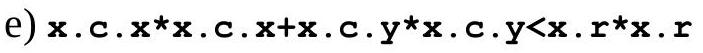
\includegraphics[max width=\textwidth, center]{2025_04_17_46e04c6acd873ea9558dg-047}\\
f) $x . r^{*} x . r<x . c . x^{*} x . c . x+x . c . y^{\star} x . c . y$\\
11. Se consideră tabloul unidimensional $\mathbf{x}=(1,2,4,3)$. Precizați care dintre următoarele variante reprezintă tabloul unidimensional $y$, știind că pentru orice $0 \leq i<4$, există relaţia $\mathbf{x}[y[i]]=y[x[i]]$.\\
a) $y=(1,2,3,4)$\\
b) $y=(1,3,4,2)$\\
c) $y=(2,3,1,4)$\\
d) $y=(3,2,1,4)$\\
e) $y=(3,4,1,2)$\\
f) $y=(4,2,1,3)$\\
12. Subprogramul $\pounds$ este definit mai jos. Precizați ce valori se vor afişa în urma apelului f('m', 0).

\begin{verbatim}
Limbajul C++/ Limbajul C
void f(char c, int x)
{
    if(!strchr("aeiou",c)){
        f(c-1,x+1)
        cout<<c;|printf("%c",c);
    }else
        cout<<x;|printf("%d",x);
}
\end{verbatim}

a) 4 jklm\\
b) 4 jmkl\\
c) 4 mlkj\\
d) $j k \operatorname{lm} 4$\\
e) jmk 14\\
c) 4 mlkj\\
f) mlkj 4

\begin{verbatim}
Limbajul Pascal
procedure f (c:char; x : word) ;
begin
if (pos(c,'aeiou')=0) then
    begin
        f(pred (c), x+1);
        write(c); end
    else write(x);
end;
\end{verbatim}

\begin{enumerate}
  \setcounter{enumi}{12}
  \item Se consideră subprogramele de mai jos. Dacă înaintea apelului $g(x)$, variabilele globale de tip întreg $\mathbf{x}$ și $\mathbf{y}$ aveau valorile 1 , respectiv -3 , precizați care vor fi valorile memorate în variabilele globale $\mathbf{x}$ și $\mathbf{y}$ după executarea apelului $\mathrm{g}(\mathbf{x})$.
\end{enumerate}

\begin{verbatim}
Limbajul C++/ Limbajul C
    void f(int x)
{ x=x+1;
\end{verbatim}

\begin{verbatim}
Limbajul Pascal
procedure f(x: longint);
begin
\end{verbatim}

\begin{verbatim}
    y=2*x+3; }
void g(int x)
{
        int a,b;
        a=x+y; b=x-y;
        f(a); f(b);
        y=y+b;
}
\end{verbatim}

a) 1 și 13\\
b) 1 și 17\\
c) 1 și 18\\
d) 2 și 13\\
e) 2 și 17\\
f) 2 și 18

\begin{verbatim}
x:=x+1;
y:=2*x+3;end;
procedure g(x: longint);
var a,b:longint;
begin
    a:=x+y; b:=x-y;
    f(a); f(b);
    y:=y+b;end;
\end{verbatim}

\begin{enumerate}
  \setcounter{enumi}{13}
  \item În secvenţa de program de mai jos, toate variabilele sunt de tip întreg. Precizați care este valoarea afișată la finalul executării secvenţei următoare.
\end{enumerate}

\begin{verbatim}
Limbajul C++/Limbajul C
$\mathrm{k}=0$;
for ( i=1;i<=9999;i++)
\{
$\mathrm{d}=2 ; \mathrm{p}=1$; $\mathrm{n}=\mathrm{i}$;
    while(d*d<=n)
    {
        e=0;
        while(n%d==0)
        {
            e++;
            n=n/d;
        }
    p=p*(e+1);
    d++;
    }
if (n>1)p=p*2;
if(p%2==0) k++;
}
    cout<<k; | printf("%d",k); write(k);
\end{verbatim}

Limbajul Pascal

\begin{verbatim}
k:=0;
for i:=1 to 9999 do
    begin
    d:=2;p:=1;n:=i;
    while d*d<=n do
        begin
        e:=0;
        while n mod d=0 do
            begin
            inc(e);
            n:=n div d;
            end;
        p:=p* (e+1);
        inc(d);
        end;
    if n>1 then p:=p*2;
    if p mod 2=0 then inc(k);
    end;
write(k);
\end{verbatim}

a) 99\\
b) 8901\\
c) 8990\\
d) 9900\\
e) 9901\\
f) 9990\\
15. Funcția $\pounds$ este definită mai jos.

\begin{verbatim}
Limbajul C++/ Limbajul C
int a[100];
int f(int x[100], int st, int dr)
{
if(st==dr) return 1;
else
    if(f(x,st,(st+dr)/2)>0&&f(x,(st+dr)/2+1,dr)>0)
        if (x[(st+dr)/2+1]>x[(st+dr)/2]) return 1;
        else return 0;
    else return 0;
}
Limbajul Pascal
type vector=array[0..99] of integer;
\end{verbatim}

\begin{verbatim}
    var a:vector;
function f(x:vector;st,dr:integer):byte;
begin
if st=dr then f:=1
else
        if (f(x,st,(st+dr) div 2)>0) and (f(x,(st+dr) div 2+1,dr)>0) then
            if x[(st+dr)div 2+1]>x[(st+dr)div 2] then f:=1
        else f:=0
    else f:=0;
end;
\end{verbatim}

Precizațic care dintre următoarele șiruri de valori pot fi memorate în tabloul unidimensional a (cu indicii începând de la 0 ), astfel încât apelul $f(a, 2,5)$ să returneze valoarea 1 .

\begin{verbatim}
1. a=(0,1,1,3,4,4,5)
2. a=(0,5,3,4,2,0)
3. a=(0,2,2,3,4,5,5)
4. a=(0,4,3,3,2,2,1)
\end{verbatim}

a) niciunul\\
b) șirurile 1 și 3\\
c) doar șirul 2\\
d) șirurile 2 și 4\\
e) doar șirul 3\\
f) toate

\section*{Varianta 10}
\begin{enumerate}
  \item Precizați ce valoare va avea variabila reală $\mathbf{x}$, după executarea următoarei instrucțiuni.
\end{enumerate}

Limbajul C++/ Limbajul C\\
$\mathbf{x}=7.51+35 / 4 * 67 \% 8-2.83$;

Limbajul Pascal\\
$\mathbf{x}:=7.51+35 \operatorname{div} 4 * 67 \bmod 8-2.83 ;$\\
a) instrucțiunea este\\
b) 4\\
c) 4.68 incorectă\\
d) 5\\
e) 28\\
f) 28.68\\
2. Precizați care dintre următoarele variante de instruncțiuni inserează cifra 2 în faţa ultimei cifre a unui număr natural n.\\
Limbajul C++/ Limbajul C

\begin{verbatim}
1. n=(n%10*10+2)*10+n/10;
2. n=(n/10*10+2)*10+n%10;
3. n=n/10+2*10+n%10;
4. }\textrm{n}=(\textrm{n}/10+2)*10+n%10
\end{verbatim}

Limbajul Pascal

\begin{verbatim}
1. n:=(n mod 10*10+2)*10+n div 10;
2. n:=(n div 10*10+2)*10+n mod 10;
3. n:=n div 10+2*10+n mod 10;
4. n:=(n div 10+2)*10+n mod 10;
\end{verbatim}

a) niciuna\\
b) 1\\
c) 1 și 2\\
d) 2\\
e) 3\\
f) 4\\
3. În secvența de program de mai jos, variabilele $\mathbf{x}, \mathbf{y}$ și $\mathbf{z}$ sunt de tip întreg.

Limbajul C++/ Limbajul C

\begin{verbatim}
z=1;
while (y>0)
{
    if(y%2)
        z=x%10*z;
    x=x*x%10;
    y=y/2;
}
cout<<z; | printf("%d",z);
\end{verbatim}

Limbajul Pascal

\begin{verbatim}
z:=1;
    while y>0 do
    begin
        if y mod %2=1 then
            z:=x mod 10*z;
        x:=x*x mod 10;
        y:=y div 2;
    end;
    write(z);
\end{verbatim}

Dacă înaintea secvenței, $\mathbf{x}$ are valoarea 137 , precizați câte valori cu exact două cifre poate avea $\mathbf{y}$ astfel încât valoarea lui $\mathbf{z}$ (afișată la finalul secvenței) să fie 1 .\\
a) 21\\
b) 22\\
c) 23\\
d) 24\\
e) 25\\
f) 26\\
4. Se consideră declarările:

\begin{verbatim}
Limbajul C++/ Limbajul C
typedef struct
    {
        float st,dr;
    } interval;
interval v[20], m;
\end{verbatim}

\begin{verbatim}
Limbajul Pascal
type interval=record
        st,dr:real;
    end;
var v:array[0..19] of interval;
m:interval;
\end{verbatim}

\begin{verbatim}
int i,j;
| i,j:word;
\end{verbatim}

Precizați care dintre următoarele instrucțiuni sunt corecte din punct de vedere sintactic.

Limbajul C++/ Limbajul C

\begin{enumerate}
  \item $v[i]=v[v[j]]$;
  \item $\mathrm{m}=(\mathrm{v}[2]+\mathrm{v}[3]) / 2$;
  \item $\mathrm{v}[10]=\mathrm{m}$;
  \item m.st=v[5].st\%2;
\end{enumerate}

Limbajul Pascal

\begin{verbatim}
1. v[i]:=v[v[j]];
2. m:=(v[2]+v[3])/2;
3. v[10]:=m;
4. m.st:=v[5].st mod 2;
\end{verbatim}

c) 1 și 4\\
a) niciuna\\
b) 1 , 2 și 3\\
d) 3\\
e) 3 și 4\\
5. Subprogramul f cu antetul int f (int x ) (în limbajul C++ și limbajul C), respectiv function $f(x$ : integer) : integer; (în limbajul Pascal), returnează cea mai mică cifră a numărului $\mathbf{x}$, care apare de cel puţin două ori în scrierea lui $\mathbf{x}$, sau valoarea -1 , dacă numărul $\mathbf{x}$ este format din cifre distincte.\\
Stabiliţi valoarea expresiei $f(f(775125)+f(97917))$.\\
a) -1\\
b) 0\\
c) 1\\
d) 12\\
e) 14\\
f) 16\\
6. Se generează prin metoda backtracking, submulţimile nevide ale mulţimii $\{1,2,3\}$ astfel: $\{1\},\{1,2\},\{1,2,3\},\{1,3\},\{2\},\{2,3\},\{3\}$. Folosind aceeaşi metodă pentru a genera submulţimile nevide ale mulţimii $\{1,2,3,4,5,6,7\}$, stabiliţi care este a $10-\mathrm{a}$, respectiv a 11-a soluție generată.\\
a) $\{1,2,3,4,7\}$,\\
b) $\{1,2,3,4,7\},\{1,2,3,5\}$\\
c) $\{1,2,3,4,6,7\}$, $\{1,2,3,6,7\}$ \{1,2,3,4,6,7\}\\
d) $\{1,2,3,4,6\}$, \{1,2,3,4,6,7\}\\
e) $\{1,2,3,4,6\}$, $\{1,2,3,5\}$\\
f) $\{1,2,3,4,6,7\},\{1,2,3,4,7\}$\\
7. Se consideră graful neorientat $G=(X, U)$ unde $X=\{1,2,3,4,5\}$ şi $\mathrm{U}=\{[1,2],[1,3],[5,1],[3,4],[4,5],[3,2]\}$. Precizați numărul minim de muchii care trebuie adăugate pentru ca graful să devină eulerian.\\
a) 0\\
b) 1\\
c) 2\\
d) 3\\
e) 4\\
f) 5\\
8. Un graf neorientat are 30 noduri şi 16 muchii. Precizați numărul componentelor conexe pe care le poate avea acest graf.\\
a) exact 14\\
b) cel puţin 14 şi cel mult 24\\
c) cel puţin 14 şi cel mult 26\\
d) cel puţin 16 şi cel mult 24\\
e) cel puţin 16 şi cel mult 26\\
f) exact 24\\
9. Fie $\mathrm{G}=(\mathrm{V}, \mathrm{E})$ un graf orientat în care mulţimea nodurilor este $\mathrm{V}=\{1,2, \ldots, 10\}$, iar mulţimea arcelor este $\mathrm{E}=\{(\mathrm{i}, \mathrm{j}) \mathrm{VxV} \mid$ i este divizor propriu al lui j$\}$. Stabiliţi care dintre următoarele afirmaţii este adevărată.

\begin{enumerate}
  \item Graful G are 3 componente tare conexe
  \item Graful G are 3 componente conexe
  \item G nu are vârfuri izolate
  \item Graful G conţine cel puțin un circuit\\
a) 1\\
b) 1 și 2\\
c) 2\\
d) 3\\
e) 4\\
f) toate
  \item Prin înălţimea unui arbore cu rădăcină înţelegem numărul de muchii ale celui mai lung lanţ elementar care are una dintre extremităţi în rădăcina arborelui. Dacă arborele este reprezentat prin următorul vector de taţi: tata $=(4,5,1,0,4,5,6,1,4)$, atunci înălţimea sa este:\\
a) 2\\
b) 3\\
c) 4\\
d) 5\\
e) 6\\
f) 7
  \item Subprogramul g este definit mai jos. Precizați ce valori se vor afișa în urma apelul g (4).
\end{enumerate}

\begin{verbatim}
Limbajul C++/ Limbajul C
void g(int n)
{int i;
    if(n>0)
    for(i=n;i>1;i--)
        {
            cout<<i; | printf("%d",i);
            g(n-2);
        }
}
\end{verbatim}

\begin{verbatim}
Limbajul Pascal
procedure g(n:word);
var i:word;
begin
if n>0 then
    for i:=n downto 2 do
    begin
        write(i);
        g(n-2);
    end;
end;
\end{verbatim}

a) 42132\\
b) 42322\\
c) 423222\\
d) 432322\\
e) 432132121\\
f) $\mathbf{4 2 1 3 2 1 2 2 1 1}$\\
12. În secvența de program alăturată, variabilele i și $\mathbf{k}$ sunt de tip întreg, iar variabila $\mathbf{A}$ memorează o matrice cu 8 linii și 8 coloane (numerotate de la 1 la 8) cu elemente numere întregi. Înainte de executarea secvenței, toate elementele vectorului sunt nule. Precizați care este a 9-a valoare afișată și care este numărul de valori afișate pe parcursul executării secvenței date.

\begin{verbatim}
Limbajul C++/ Limbajul C
n=8;k=3;
for (i=n;i>=1;i--)
        for(j=n;j>=1;j--)
            A[i][j]=n*(j-1)+i;
for(i=k;i<=n-k+1;i++)
    cout<<A[i][k]<<' '; | printf("%d ", A[i][k]);
for(i=k+1;i<=n-k+1;i++)
    cout<<A[n-k+1][i]<<' '; | printf("%d ",A[n-k+1][i]);
for(i=n-k;i>=k;i--)
    cout<<A[i][n-k+1]<<' '; | printf("%d ", A[i][n-k+1]);
for(i=n-k;i>k;i--)
    cout<<A[k][i]<<' '; | printf("%d ", A[k][i]);
\end{verbatim}

Limbajul Pascal\\
$\mathrm{n}:=8 ; \mathrm{k}:=3$;\\
for i:=n downto 1 do\\
for $\mathrm{j}:=\mathrm{n}$ downto 1 do

\begin{verbatim}
            A[i,j]:=n*(j-1)+i;
for i:=k to n-k+1 do
        write(A[i,k],' ');
for i:=k+1 to n-k+1 do
    write(A[n-k+1,i],' ');
for i:=n-k downto k do
    write(A[i,n-k+1],' ');
for i:=n-k downto k+1 do
        write(A[k,i],' ');
\end{verbatim}

a) $\mathbf{4 3}$ și $\mathbf{1 0}$\\
b) 43 și 12\\
C) 44 și 10\\
d) 44 și 12\\
e) 45 și 10\\
f) 45 și 12\\
13. Se consideră declarările:

\begin{verbatim}
Limbajul C++/ Limbajul C
char s[30]="bacaacbc";
char t[3][3]={"ab","ac","bc"};
\end{verbatim}

\begin{verbatim}
Limbajul Pascal
var i:word;
s:string[30];
t:array[0..2]of string[3];
\end{verbatim}

Precizați ce se va afișa după executarea secvenței de program de mai jos.

\begin{verbatim}
Limbajul C++/ Limbajul C
for(int i=0;i<3;i++)
    if (!strstr(s,t[i]))
        strcat(s,t[2-i]);
    else cout<<t[i]; | printf("%s",t[i]);
cout<<strlen(s); | printf("%d",strlen(s));
cout<<s; | printf("%s",s);
\end{verbatim}

Limbajul Pascal

\begin{verbatim}
s:='bacaacbc';t[0]:='ab';t[1]:='ac';t[2]:='bc';
for i:=0 to 2 do
        if pos(t[i],s)=0 then s:=s+t[2-i]
        else write(t[i]);
write(length(s));
write(s);
\end{verbatim}

a) secvența este incorectă\\
b) acbc8bacaacbc\\
C) acbc10bacaacbc sintactic\\
d) bcac10bacaacbcbc\\
e) $a c b 10 b a c a a c b c b c$\\
f) $a c b c 10 b a c a a c b c b c$\\
14. Subprogramul p este definit mai jos. Variabila a memorează un vector cu 100 de elemente numere întregi, aflate pe poziții numerotate de la o la 99. Precizaţi câte elemente divizibile cu 3 conține tabloul unidimensional a după executarea apelului $p(6, a)$.

\begin{verbatim}
Limbajul C++/Limbajul C
void p(int k, int v[100])
{ int w[100];
    v[0]=w[0]=1;
    for(int i=1;i<=k;i++)
    {
        for(int j=0;j<=i;j++)
        {
            if(j==0) v[j]=1;
            else
            if(i==j) v[j]=1;
\end{verbatim}

\begin{verbatim}
Limbajul Pascal
type vector=array[0..99]of integer;
var a:vector;
procedure p(k:integer; var v:vector);
var w:vector; i,j:integer;
begin
    v[0]:=1; w[0]:=1;
    for i:=1 to k do begin
        for j:=0 to i do
            if j=0 then v[j]:=1
                else
\end{verbatim}

\begin{verbatim}
                else v[j]=w[j-1]+w[j];
        }
        for(int j=0;j<=i;j++)
            w[j]=v[j];
    }
}
\end{verbatim}

\begin{verbatim}
    if i=j then v[j]:=1
        else v[j]:=w[j-1]+w[j];
    for j:=0 to i do w[j]:=v[j];
    end;
end;
\end{verbatim}

a) 1\\
b)2\\
c) 3\\
d) 4\\
e) 5\\
f) 6\\
15. Variabilele $\mathbf{x}, \mathrm{n}, \mathbf{i}, \mathrm{b}, \mathrm{c}$ memorează numere naturale. Dacă inițial variabila b memorează valoarea 3 și variabila x memorează inițial valoarea 0 , indicaţi valoarea afișată de secvența de program următoare:

\begin{verbatim}
Limbajul C++/ Limbajul C
for(i=0;i<=99;i++)
{
    c=0,n=i;
    while(n>0)
    {
        c=c+n%b;
        n=n/b;
    }
    if(c>x) x=c;
}
cout<<x; l printf("%d",x);
\end{verbatim}

a) 4\\
b) 5\\
c) 6\\
d) 7\\
e) 8\\
f) 9

\begin{verbatim}
Limbajul Pascal
for i:=0 to 99 do
    begin
        c:=0;n:=i;
        while n>0 do
            begin
            c:=c+n mod b;
            n:=n div b;
            end;
            if c>x then x:=c;
end;
write(x);
\end{verbatim}

\section*{Varianta 11}
\begin{enumerate}
  \item Precizaţi care este numărul elementelor egale cu 1 (pentru limbajul $\mathbf{C} / \mathbf{C}++$ )/true (pentru limbajul Pascal) aflate pe diagonala principală în urma executării secvenței de mai jos, în care a este un tablou bidimensional cu $\mathbf{n}$ linii și $\mathbf{n}$ coloane, iar $\mathbf{i}, \mathbf{j}$ sunt variabile de tip întreg.
\end{enumerate}

\begin{verbatim}
Limbajul C++
for(i=n;i>=1;i--)
for(j=n;j>=1;j--)
    a[i][j]=(i==j);
\end{verbatim}

a) nu poate fi calculat\\
b) $n^{2}$

\begin{verbatim}
Limbajul C
for(i=n;i>=1;i--)
for(j=n;j>=1;j--)
    a[i][j]=(i==j);
\end{verbatim}

Limbajul Pascal for $i:=n$ downto 1 do for $j:=n$ downto 1 do\\
$a[i, j]:=(i=j) ;$\\
c) $\mathrm{n}-1$\\
d) $n^{2}-1$\\
e) $n$\\
f) $(\mathrm{n}+1) * \mathrm{n} / 2$\\
2. Precizaţi care este complexitatea algoritmului de interclasare a două șiruri, cu m și respectiv n numere naturale ( $\mathrm{n} \leq \mathrm{m}$ ).\\
a) $O(\max (m, n))$\\
b) $O(\min (m, n))$\\
c) $O(m+n)$\\
d) $O(m * n)$\\
e) $O\left(\operatorname{llog}_{2}(n)\right)$\\
f) $O\left(\mathrm{nlog}_{2}(\mathrm{~m})\right)$\\
3. Indicaţi care dintre următoarele secvențe de program calculează în variabila nr, în mod corect și eficient ca timp de executare, numărul cuburilor naturale perfecte mai mici sau egale decât $\mathbf{n}$ (număr natural cunoscut).\\
a)

\begin{verbatim}
Limbajul C++
int n,nr=0,i;
cin>>n;
for(i=1;i<=n;i++)
if(i*i*i<=n)
nr++;
cout<<nr;
\end{verbatim}

b)

\begin{verbatim}
Limbajul C++
int n,nr=0,i,j;
cin>>n;
for(i=1;i<=n;i++)
for(j=1;j<=i;j++)
if(j*j*j==i)
nr++;
cout<<nr;
\end{verbatim}

\begin{verbatim}
Limbajul C
int n,nr=0,i;
scanf("%d",&n);
for(i=1;i<=n;i++)
if(i*i*i<=n)
nr++;
printf("%d",nr);
\end{verbatim}

\begin{verbatim}
Limbajul Pascal var n,i,nr:integer; BEGIN readln(n); nr:=0;
    for i:=1 to n do
if i*i*i<=n then
nr:=nr+1;
writeln(nr);
END.
\end{verbatim}

\begin{verbatim}
Limbajul C
int n, nr=0, j, i;
scanf("%d",&n);
for(i=1;i<=n;i++)
for(j=1;j<=i;j++)
if(j*j*j==i)
nr++;
printf("%d",nr);
\end{verbatim}

\begin{verbatim}
Limbajul Pascal
var
n,nr,i,j:integer;
BEGIN
readln(n);nr:=0;
for i:=1 to n do
for j:=1 to i do
if j*j*j=i then
nr:=nr+1;
writeln(nr);
END.
\end{verbatim}

c)

\begin{verbatim}
Limbajul C++
int n,nr;
cin>>n;
nr=(int) exp(1/2.0*
log(n));
cout<<nr;
\end{verbatim}

d)

\begin{verbatim}
Limbajul C++
int n, nr;
cin>>n;
nr=n*n* (n+1)*(n+1)/4;
cout<<nr;
\end{verbatim}

e)

\begin{verbatim}
Limbajul C++
int n, nr;
cin>>n;
nr=n*n* (n+1)* (n+1)/6;
cout<<nr;
\end{verbatim}

f)

\begin{verbatim}
Limbajul C++
int n, nr;
cin>>n;
nr=(int) exp(1/3.0*
log(n));
cout<<nr;
\end{verbatim}

\begin{verbatim}
Limbajul C
int n,nr;
scanf("%d",&n);
nr=(int) exp(1/2.0*
log(n));
printf("%d",nr);
\end{verbatim}

\begin{verbatim}
Limbajul Pascal
var n,nr:integer;
BEGIN
readln(n);
nr:=trunc (exp (1/2*
ln(n)));
writeln(nr) ;
END.
\end{verbatim}

\begin{verbatim}
Limbajul C
int n, nr;
scanf("%d",&n);
nr=n*n* (n+1) * (n+1)/4;
printf("%d",nr);
\end{verbatim}

\begin{verbatim}
Limbajul Pascal
var n, nr:integer;
BEGIN
readln(n) ;
nr:=n*n* (n+1)* (n+1) div 4;
writeln(nr) ;
END.
\end{verbatim}

\begin{verbatim}
Limbajul C
int n, nr;
scanf("%d",&n);
nr=n*n* (n+1)* (n+1) / 6;
printf("%d",nr);
\end{verbatim}

\begin{verbatim}
Limbajul Pascal
var n, nr:integer;
BEGIN
readln(n) ;
nr:=n*n*(n+1)*(n+1) div 6;
writeln(nr) ;
END.
\end{verbatim}

\begin{verbatim}
Limbajul C
int n, nr;
scanf("%d",&n);
nr=(int) exp(1/3.0*
log(n));
printf("%d",nr);
\end{verbatim}

\begin{verbatim}
Limbajul Pascal
var n, nr:integer;
BEGIN
readln(n);
nr:=trunc (exp (1/3*
ln(n)));
writeln(nr) ;
END.
\end{verbatim}

\begin{enumerate}
  \setcounter{enumi}{3}
  \item Se definește funcția:\\
$M_{n}^{k}=\left\{\begin{array}{c}M_{n-1}^{k}+k * M_{n-1}^{k-1} \text { pentru } k>0 \\ 1 \text { pentru } k=0\end{array}\right.$\\
Dacă se citesc numerele naturale $\mathbf{n}, \mathbf{k}(\mathbf{n}>=\mathbf{k})$ și se apelează funcția recursivă scrisă într-un limbaj de programare cunoscut (C++/C sau Pascal) care evaluează funcția definită mai sus, valoarea calculată reprezintă:\\
a) produsul cartezian\\
d) numărul submulțimilor cu b) numărul submulțimilor\\
unei mulțimi cu n elemente\\
c) afișarea tuturor aranjamentelor mulțimii $\{1,2, . . . n\}$ luate câte $\mathbf{k}$ $\mathbf{k}$ elemente ale unei mulțimi\\
e) afiṣarea tuturor f) nici una dintre aceste cu $n$ elemente combinărilor mulțimii variante
  \item Indicaţi care este efectul prelucrării secvenței de program de mai jos, pentru $\mathbf{x}, \mathbf{y}$ numere naturale cu $\mathbf{x} \leq \mathbf{y}$ :
\end{enumerate}

\begin{verbatim}
Limbajul C++
int f(int x,int
y) {
if(x==y) return x;
else if(x>y)
return x-1;
else
return
    f(++x,--y);}
int main()
{int x, y;
cin>>x>>y;
    cout<<f(x,y);
return 0;}
\end{verbatim}

\begin{verbatim}
Limbajul C
int f(int x,int
y) {
if(x==y) return x;
else if(x>y)
return x-1;
else
return
f(++x,--y) ;}
int main()
{int x, y;
scanf("%d%d",&x,&y);
printf("%d",f(x,y));
return 0;}
\end{verbatim}

\begin{verbatim}
Limbajul Pascal
var x,y:integer;
function
f(x,y:integer):integ
er;
begin
if x=y then f:=x
else
if x>y then f:=x-1
else
f:=f(succ(x),pred(y))
end;
begin
readln(x,y);
writeln(f(x,y));
end.
\end{verbatim}

S-a notat cu [a] partea întreagă a numărului a și cu |a-b|, modulul diferenței a-b.\\
a) $\mathbf{x}+\mathbf{y}$\\
b) $[y-x]$\\
c) $|y-x|$\\
d) $\mathbf{x}^{y}$\\
e) $[(x+y) / 2]$\\
f) $y^{x}$\\
6. Indicaţi care este valoarea inițială a variabilei a dacă, în urma executării secvenței următoare de program, s-a afișat valoarea 6.

\begin{verbatim}
Limbajul C++
int a=... ,n;
n=16327;
while(n!=0)
{
switch(n%10) {
case 0: case 2: case
4:case 6: case 8:
a=a+n%2;break;
case 1: case 3: case
5:case 7: case 9:
a=a-n%2; break;}
n=n/10;
}
cout<<<a<<endl;
\end{verbatim}

a) 8\\
b) nici una dintre\\
variante variante

\begin{verbatim}
Limbajul C
    int a=... ,n;
n=16327;
while(n!=0)
{
switch(n%10) {
case 0: case 2:
case 4:case 6:
case 8:
a=a+n%2;break;
case 1: case 3:
case 5:case 7:
case 9: a=a-n%2;
break;}
n=n/10;
}
printf("%d",a);
\end{verbatim}

\begin{verbatim}
Limbajul Pascal
var n,a:integer;
BEGIN
a:=...;
n:=16327;
while n>0 do
begin
case n mod 10 of
0,2,4,6,8:
a:=a+n mod 2;
1,3,5,7,9:
a:=a-n mod 2;
end;
n:=n div 10;
end;
writeln(a);
END.
\end{verbatim}

c) 9\\
d) 13\\
e)10\\
f) 5\\
7. Fie un graf neorientat conex cu $\mathbf{4 0}$ de noduri și $\mathbf{7 0}$ de muchii. Precizați numărul maxim de muchii care pot fi eliminate astfel încât graful să rămână conex:\\
a) 31\\
b) 30\\
c) 1\\
d) 0\\
e) 39\\
f) 35\\
8. Precizați numărul grafurilor orientate complete cu noduri care pot fi construite:\\
a) $4^{n \star(n-1) / 2}$\\
b) $4^{n}(\mathrm{n}+1) / 2$\\
c) $3^{n \star(n+1) / 2}$\\
d) $\mathbf{4}^{\mathrm{n} / 2}$\\
e) $2^{\mathrm{n}^{\star}(\mathrm{n}-1) / 2}$\\
f) $3^{n \star(n-1) / 2}$\\
9. Precizați care din următoarele șiruri de numere nu poate reprezenta gradele vârfurilor unui arbore.\\
a) 2211\\
b) 411211\\
c) 121\\
d) 111215\\
e) 111214\\
f) 121213\\
10. Precizați care este valoarea produsă de subprogramului $\mathbf{f}$ definit mai jos, în urma apelului $\mathbf{f ( s )}$, atunci când parametrul $\mathbf{s}$ primește șirul de caractere: 123abc4567

\begin{verbatim}
Limbajul C++
int f( char s[100])
{int i, nr=0, n=strlen(s);
for(i=0;s[i]>='0'&&s[i]<='9';i++)
    nr=nr*10+s[n-i-1]-'0';
return nr;}
\end{verbatim}

\begin{verbatim}
Limbajul C
int f( char s[100])
{int nr=0,i,n;
n=strlen(s);
for(i=0;s[i]>='0'&&s[i]<='9';i++)
    nr=nr*10+s[n-i-1]-'0';
    return nr;}
\end{verbatim}

\begin{verbatim}
Limbajul Pascal
function f(s:String):longint;
var n,nr,i:longint ;
begin
n:=Length(s);nr:=0;i:=1;
while (s[i]>='0') and (s[i]<='9') do
begin
nr:=10*nr+ord(s[n-i+1])-ord('0');
i:=i+1;
end;f:=nr;
end;
\end{verbatim}

a) 1234567\\
b) 123\\
c) 456\\
d) 321\\
e) 765\\
f) 7654\\
11. Precizați care este suma calculată în urma apelului $f(1, n)$ al subprogramului $f$ definit mai jos, unde $n$ este un număr natural cunoscut:

\begin{verbatim}
Limbajul C++
int f(int i, int n)
{
    if(i<=3*n)
        if(i%3!=0)
            return f(i+1,n);
        else
            return i+f(i+1,n);
        else return 0;
}
\end{verbatim}

\begin{verbatim}
Limbajul C
int f(int i, int n)
{
    if(i<=3*n)
        if(i%3!=0)
            return f(i+1,n);
        else
            return i+f(i+1,n);
    else return 0;
}
\end{verbatim}

\begin{verbatim}
Limbajul Pascal
function f(i,n:integer):integer;
begin
if i<=3*n then
    if i mod 3 =0 then
        f:=f(i+1,n)+i
    else f:=f(i+1,n)
else f:=0
end;
\end{verbatim}

a) $\sum_{i=1}^{3 n} i$\\
b) $\sum_{i=1}^{n} 3 * i$\\
c) $\sum_{i=1}^{n} \boldsymbol{i}$\\
d) $\sum_{i=1}^{n}(i+3)$\\
e) $\sum_{i=1}^{n} \boldsymbol{i} / \mathbf{3}$\\
f) $\sum_{i=1}^{n / 3} i$\\
12. Utilizând metoda backtracking, se generează toate posibilitățile de a forma șiruri din trei cuvinte distincte din mulțimea \{examen, reușit, promovat, nota, felicitări\}. Primele trei soluții sunt: examen reușit promovat; examen reușit nota; examen reușit felicitări. Indicați care este soluția generată înainte de felicitări examen reușit.\\
a) nota examen felicitări\\
b) nota felicitări promovat\\
c) felicitări examen promovat\\
d) examen promovat\\
e) felicitări nota examen\\
f) promovat examen felicitări felicitări\\
13. Dacă pentru variabila a se citește valoarea 11, precizați câte valori pot fi citite pentru variabila b astfel încât în urma apelului $\mathbf{f}(\mathbf{a}, \mathbf{b})$, subprogramul $\mathbf{f}$ de finit mai jos să producă valoarea 10.

\begin{verbatim}
Limbajul C++
int f(int a,int b)
{ if(a==b)
        return a%2;
    else
return
f(a,(a+b)/2)+f((a+b)/2+1,b); }
\end{verbatim}

\begin{verbatim}
Limbajul C
int f(int a,int b)
{ if(a==b)
        return a%2;
    else
return
f(a, (a+b)/2) +f((a+b)/2+1,b) ;}
\end{verbatim}

\begin{verbatim}
Limbajul Pascal
function f(a,b:integer):integer;
begin
if a=b then f:=a mod 2
else
f:=f(a,(a+b) div 2) +f((a+b) div 2+1,b);
end;
\end{verbatim}

a) 2\\
b) 1\\
c) 0\\
d)3\\
e) 4\\
f) 7\\
14. Indicați pentru ce valori ale lui $\mathbf{n}$ și $\mathbf{p}$, valoarea variabilei întregi $\mathbf{x}$ este 164 , în urma apelului $f(1)$ al subprogramului $f$ definit mai jos.

\begin{verbatim}
Limbajul C++
int s[100],n,p,x;
void f(int k)
{ int i;
    if(k==p+1) x++;
\end{verbatim}

\begin{verbatim}
Limbajul C
int s[100],n,p,x;
void f(int k)
{ int i;
    if(k==p+1) x++;
\end{verbatim}

\begin{verbatim}
else
if(k==1)
for(i=1;i<=n;i++) f(k+1);
    else
for(i=1+s[k-1];i<=n;i++)
    { s[k]=i;f(k+1); }}
\end{verbatim}

\begin{verbatim}
else
if(k==1)
for(i=1;i<=n;i++) f(k+1);
        else
    for(i=1+s[k-1];i<=n;i++)
        { s[k]=i;f(k+1); }}
\end{verbatim}

Limbajul Pascal\\[0pt]
type vector=array[1..100] of integer;\\
var $\mathrm{n}, \mathrm{p}, \mathrm{x}$ :integer;\\
s: vector;\\
procedure $f(k$ :integer) ;\\
var i,il:integer;\\
begin\\
if $k=p+1$ then $x:=x+1$\\
else\\
if $k=1$ then\\
for il:=1 to $n$ do\\
begin\\[0pt]
s[k]:=i1; $f(k+1)$;\\
end\\
else\\
for $i:=1+s[k-1]$ to $n$ do\\
begin\\[0pt]
s[k]:=i; $\mathrm{f}(\mathrm{k}+1)$;\\
end; end;\\
a) 82 și 2\\
b) 164 și 1\\
c) 328 și 4\\
d) 41 si 123\\
e) 41 și 1\\
f) 81 și 2\\
15. Precizați care este valoarea produsă de subprogramul $f$, definit mai jos, în urma apelului f(1999, 7) .

\begin{verbatim}
Limbajul C++
int f(int x, int n)
{if(n)
if(n%2==0)
return (f(x,n/2)*f(x,n/2)) % 10;
else
return (x*f(x,n-1))%10;
    else
return 1;}
\end{verbatim}

\begin{verbatim}
Limbajul C
int f(int x, int n)
{if(n)
    if(n%2==0)
return
(f(x,n/2)*f(x,n/2))%10;
else
return (x*f(x,n-1))%10;
    else
return 1;}
\end{verbatim}

\begin{verbatim}
Limbajul Pascal
function f(x,n:integer):integer;
begin
if n=0 then f:=1
else
if n mod 2=0 then
\end{verbatim}

\begin{verbatim}
f:=(f(x,n div 2)*f(x,n div 2)) mod 10
else
    f:=(x*f(x,n-1)) mod 10;
end;
\end{verbatim}

a) 798800599919\\
b) 9\\
c) nu poate fi\\
d) 1\\
e) 0\\
f) 28

\begin{verbatim}

\end{verbatim}

\section*{Varianta 12}
\begin{enumerate}
  \item Precizați care este numărul muchiilor care trebuie adăugate, îtr-un graf neorientat conex care are $\mathbf{n}$ noduri și $\mathrm{n}-1$ muchii ( n număr natural cunoscut), pentru a deveni complet:\\
a) $n *(n-1) / 2$\\
b) $(n-1) *(n-2) / 2$\\
c) $n$\\
d) $(\mathrm{n}+1) * \mathrm{n} / 2$\\
e) 0\\
f) $n-1$
  \item În secvenţa următoare $\mathbf{i}, \mathbf{j}$ şi $\mathbf{n}$ sunt variabile întregi, iar a este un tablou bidimensional format din $\mathbf{n}$ linii şi $\mathbf{n}$ coloane numerotate de la 1 la $\mathbf{n}$. Indicați care este suma elementelor de pe diagonala secundară a tabloului a, în urma executării acestei secvențe.
\end{enumerate}

\begin{center}
\begin{tabular}{l|l|l}
Limbajul C++ & Limbajul C & Limbajul Pascal \\
for $(i=1 ; i<=n ; i++)$ & for $(i=1 ; i<=n ; i++)$ & for $i:=1$ to $n$ do \\
for $(j=1 ; j<=n ; j++)$ & for $(j=1 ; j<=n ; j++)$ & for $j:=1$ to $n$ do \\
a[i][j] =(i+j)\% n; & a[i][j]=(i+j)\% $n ;$ & $a[i, j]:=(i+j) \bmod n ;$ \\
\end{tabular}
\end{center}

a) $n$\\
b) $n-1$\\
c) nu se poate calcula\\
d) $(n+1) * n / 2$\\
e) $n^{2}$\\
f) $n * n$\\
3. Indicați care dintre următoarele secvențe de program calculează în variabila nr, în mod corect și eficient ca timp de executare, suma primelor n cuburi naturale perfecte nenule ( $n$ număr natural cunoscut).\\
a)

\begin{verbatim}
Limbajul C++
int n, nr=0, i;
cin>>n;
for(i=1;i<=n;i++)
if(i*i*i<=n)
nr+=i*i*i;
cout<<nr;
\end{verbatim}

\begin{verbatim}
Limbajul C int $\mathrm{n}, \mathrm{nr}=0$, i ; scanf("\%d", \&n);
for(i=1;i<=n;i++)
if(i*i*i<=n)
nr+=i*i*i;
printf("%d",nr);
\end{verbatim}

\begin{verbatim}
Limbajul Pascal var n , nr,i:integer;
BEGIN readln(n); nr:=0;
    for i:=1 to n do
if i*i*i<=n then
nr:=nr+i*i*i;
writeln(nr);
END.
\end{verbatim}

b)

\begin{verbatim}
Limbajul C++
int n, nr=0, i, j;
cin>>n;
for(i=1;i<=n;i++)
for(j=1;j<=i;j++)
if(j*j*j==i)
nr+=i*i*i;
cout<<nnr;
\end{verbatim}

c)

\begin{center}
\begin{tabular}{l|l|l}
Limbajul C++ & Limbajul C & Limbajul Pascal \\
int $n, \mathrm{nr} ;$ & int $\mathrm{n}, \mathrm{nr} ;$ & var $\mathrm{n}, \mathrm{nr}$ :integer; \\
\end{tabular}
\end{center}

\begin{verbatim}
cin>>n;
nr=(int) exp(1/3.0*
log(n));
cout<<nr;
\end{verbatim}

d)

\begin{verbatim}
Limbajul C++
int n, nr;
cin>>n;
nr=n*n* (n+1)*(n+1)/4;
cout<<nr;
\end{verbatim}

e)

\begin{verbatim}
Limbajul C++
int n, nr;
cin>>n;
nr=(int) exp(1/2.0*
log(n));
cout<<nr;
\end{verbatim}

f)

\begin{verbatim}
Limbajul C++
int n, nr;
cin>>n;
nr=n*n* (n+1)* (n+1)/6;
cout<<nr;
\end{verbatim}

\begin{verbatim}
scanf("%d",&n);
nr=(int) exp (1/3.0*
log(n)));
printf("%d",nr) ;
\end{verbatim}

\begin{verbatim}
BEGIN
readln(n);
nr:=trunc (exp (1/3*
ln(n)));
writeln(nr);
END .
\end{verbatim}

\begin{verbatim}
int n, nr;
scanf("%d",&n);
nr=n*n* (n+1) * (n+1) /4;
printf("%d",nr) ;
\end{verbatim}

Limbajul C

\begin{verbatim}
Limbajul Pascal
var n, nr:integer;
BEGIN
readln(n);
nr:=n*n* (n+1) * (n+1)
div 4;
writeln(nr) ;
END .
\end{verbatim}

\begin{verbatim}
Limbajul C
int n, nr;
scanf("%d",&n);
nr=(int) exp (1/2.0*
log(n)));
printf("%d",nr) ;
\end{verbatim}

\begin{verbatim}
Limbajul Pascal
var n, nr:integer;
BEGIN
readln(n);
nr:=trunc (exp (1/2*
ln(n)));
writeln(nr) ;
END .
\end{verbatim}

Limbajul C

\begin{verbatim}
int n, nr;
scanf("%d",&n) ;
nr=n*n* (n+1) * (n+1) /6;
printf("%d",nr) ;
\end{verbatim}

\begin{verbatim}
Limbajul Pascal
var n, nr:integer;
BEGIN
readln(n);
nr:=n*n* (n+1) * (n+1)
div 6;
writeln(nr) ;
END .
\end{verbatim}

\begin{enumerate}
  \setcounter{enumi}{3}
  \item Se definește recursiv o funcție care calculează numărul combinărilor de $\mathbf{n}$ luate câte $\mathbf{k}$ astfel: $\quad C_{n}^{k}=\left\{\begin{array}{c}\frac{n-k+1}{k} * C_{n}^{k-1} \text { pentru } k>0 \\ 1 \text { pentru } k=0\end{array}\right.$\\
Dacă se citesc numerele naturale $n, k(n>=k)$ și se apelează funcția recursivă scrisă întrun limbaj de programare cunoscut (C++/C/Pascal) care evaluează funcția definită mai sus, precizați care este numărul apelurilor necesare pentru a calcula $\boldsymbol{C}_{\boldsymbol{n}}^{\boldsymbol{k}}$ :\\
a) $n$\\
b) $k$\\
c) $\mathbf{k - 1}$\\
d) $n+1$\\
e) $\mathrm{n}+\mathbf{k}$\\
f) $k+1$
  \item Precizați numărul circuitelor care trec prin toate nodurile unui graf orientat tare conex cu n noduri ( n număr natural cunoscut).\\
a) cel puțin 1\\
b) exact 1\\
c) 0\\
d) cel mult 1\\
e) exact n-2\\
f) exact $\mathbf{n + 1}$
  \item Precizați ce afișează următoarea secvență de program:
\end{enumerate}

\begin{verbatim}
Limbajul C++
    int a=0,n;
            cin>>n;
        do
{
switch(n%10)
{
    case 0: case 2:
case 4:case 6:
case 8:
a=a-(n%2) *(n%10);
break;
case 1: case 3:
case 5:case 7: case
9:
a=a+(n%2) *(n%10);
break;
}
n=n/10;
} while(n!=0);
cout<<a<<endl;
\end{verbatim}

a) suma cifrelor numărului $n$\\
d) numărul cifrelor prime din numărul n

\begin{verbatim}
Limbajul C
int a=0,n;
scanf("%d",&n);
    do
    {
switch(n%10)
{
    case 0: case 2:
case 4:case 6:
case 8:
a=a-(n%2) *(n%10);
break;
    case 1: case 3:
case 5:case 7: case
9:
a=a+(n%2) *(n%10);
break;
}
n=n/10;
} while(n!=0);
printf("%d",a);
\end{verbatim}

b) numărul cifrelor impare din numărul n\\
e) suma cifrelor impare din numărul $n$

\begin{verbatim}
Limbajul Pascal
var n,a:integer;
BEGIN
a:=0;
readln(n);
while n>0 do
begin
case n mod 10 of
0,2,4,6,8:
a:=a-(n mod 2)*
(n mod 10);
1,3,5,7,9:
    a:=a+(n mod 2)*
(n mod 10);
end;
n:=n div 10;
end;
        writeln(a);
END.
\end{verbatim}

c) diferența dintre suma cifrelor pare și suma cifrelor impare din numărul n\\
f) diferența dintre suma cifrelor impare și suma cifrelor pare din numărul $n$\\
7. Folosind metoda backtracking se generează toate șirurile formate din patru caractere distincte din mulțimea $\{\#, *, \&, @, \%$ \}. Primele trei soluții sunt: \#\textit{\&@, \#}\&\%, \#*@\&. Indicați care este soluția generată înainte de $\& *$ \#@\\
a) $\& @ \%$ \#\\
b) $\& \# @ \%$\\
c) $\& \# \%$ @\\
d) $* \& @ \%$\\
e) $* \& \%$ @\\
f) $\& @ \# \%$\\
8. Un graf orientat se numește turneu, dacă între oricare două vârfuri i şi j, ījj, există un singur arc. Precizați numărul grafurilor turneu cu n noduri ( n număr natural cunoscut).\\
a) $4^{n \star(n-1) / 2}$\\
b) $3^{n}(n-1) / 2$\\
c) $4^{n *(n+1) / 2}$\\
d) $2^{n \star(n-1) / 2}$\\
e) $2^{n \star(n+1) / 2}$\\
f) $3^{n \star(n+1) / 2}$\\
9. Precizați care din următoarele șiruri de numere poate reprezenta gradele vârfurilor unui arbore cu n noduri ( n număr natural cunoscut).\\
a) 411211\\
b) 2111\\
c) 122\\
d) 111215\\
e) 111\\
f) 111216\\
10. Precizați care este valoarea produsă de subprogramul f, definit mai jos, în urma apelului $\mathrm{f}(\mathrm{s})$, atunci când variabila s memorează șirul de caractere: 123abc45678

\begin{verbatim}
Limbajul C++
int f( char s[100])
{int nr=0,i,n=strlen(s) ,p=1;
for(i=0;s[i]>='0'&&s[i]<='9'; i++)
    {nr=nr+p*(s[n-i-1]-'0');
        p*=10;}
return nr;
}
\end{verbatim}

\begin{verbatim}
Limbajul C
int f( char s[100])
{int nr=0,i,
n=strlen(s),p=1;
for(i=0;s[i]>='0'&&s[i]<='9'; i++)
{nr=nr+p*(s[n-i-1]-'0');
    p*=10;}
return nr;}
\end{verbatim}

\begin{verbatim}
Limbajul Pascal
function f(s:String):longint;
var n,nr,i,p:longint;
begin
n:=Length(s) ;nr:=0;i:=1;p:=1;
while (s[i]>='0') and (s[i]<='9') do
begin
nr:=nr+p*(ord(s[n-i+1])-ord('0'));
i:=i+1; p:=p*10;
end;f:=nr;
end;
\end{verbatim}

a) 45678\\
b) 123\\
c) 876\\
d) 678\\
e) 654\\
f) 876\\
11. În urma apelului $f(1, n)$ al subprogramului $f$ definit mai jos, este calculată valoarea sumei...:

\begin{verbatim}
Limbajul C++
float f(int i,int
n)
{ if(i<=3*n)
            if(i%3!=0)
    return f(i+1,n);
        else
return
1.0/i+f(i+1,n);
        else return 0;}
\end{verbatim}

\begin{verbatim}
Limbajul C
float f(int i,int
n)
{ if(i<=3*n)
        if(i%3!=0)
    return f(i+1,n);
        else
return
1.0/i+f(i+1,n);
    else return 0;}
\end{verbatim}

a)\\
) b)\\
$\sum_{i=1}^{n} 1 /(3 * i)$\\
c)\\
d)\\
$\sum_{i=1}^{n} 1 / i$\\
$\sum_{i=1}^{2 n} 1 / i$

\begin{verbatim}
Limbajul Pascal
function
f(i,n:integer):double;
begin
if i<=3*n then
if i mod 3=0 then
f:=f(i+1,n)+1/i
else f:=f(i+1,n)
else f:=0
end;
e) f)
$\sum_{i=1}^{n} 1 /(i-3) \quad \sum_{i=1}^{n} 1 /(i+3)$
\end{verbatim}

\begin{enumerate}
  \setcounter{enumi}{11}
  \item Precizați care este valoarea variabilei $\mathbf{x}$, în urma apelului $\mathbf{f}(1)$ al subprogramului $\mathbf{f}$ definit mai jos, pentru $n=4$ și $p=3$.
\end{enumerate}

\begin{verbatim}
Limbajul C++
int s[100],n,p,x;
void f(int k)
{ int i,j,ok;
if(k==p+1) x++;
    else
for(i=1;i<=n;i++)
{s[k]=i;
ok=1;
\end{verbatim}

\begin{verbatim}
Limbajul C
int s[100],n,p,x;
void f(int k)
{int i,j,ok;
if(k==p+1) x++;
    else
for(i=1;i<=n;i++)
{s[k]=i;
ok=1;
\end{verbatim}

\begin{verbatim}
Limbajul Pascal
type
vector=array[1..100]
of integer;
var n,p,x:integer;
s: vector;
procedure
f(k:integer);
\end{verbatim}

\begin{verbatim}
for(j=1;j<k;j++)
if(s[k]==s[j])
ok=0;
if(ok) f(k+1);
} }
\end{verbatim}

\begin{verbatim}
for(j=1;j<k;j++)
if(s[k]==s[j])
ok=0;
if(ok) f(k+1);
} }
\end{verbatim}

\begin{verbatim}
var i,il,j,ok:integer;
begin
if k=p+1 then
x:=x+1
else
if k=1 then
    for il:=1 to n do
        begin
            s[k]:=i1; f(k+1);
        end
else
for i:=1 to n do
    begin
            s[k]:=i;
        ok:=1;
        for j:=1 to k-1 do
            if s[k]=s[j] then
                ok:=0;
        if ok=1 then f(k+1);
    end; end;
\end{verbatim}

a) 120\\
b) 12\\
c) 10\\
d) 8\\
e) 24\\
f) 60\\
13. Precizați numărul maxim de muchii care pot exista într-un graf neorientat cu $\mathbf{n}$ noduri ( $\mathbf{n}$ număr natural cunoscut):\\
a) $n$\\
b) $n *(n+1) / 2$\\
c) $n *(n-1) / 2$\\
d) $n * n *(n-1)$\\
e) $n+1$\\
f) $n-1$\\
14. Dacă pentru variabila n se citește valoarea 12 , precizați care este valoarea produsă în urma apelului $f(1, n, n)$ al subprogramului $\mathbf{f}$ definit mai jos:

\begin{verbatim}
Limbajul C++
int f(int a,int b, int n)
{
if(a==b)
    return (n%a==0?1:0);
else
return
f(a,(a+b)/2,n)+f((a+b)/2+1,b,n); }
Limbajul C
int $f($ int $a, i n t b, i n t n)$
\{
if ( $a==b$ )
    return (n%a==0?1:0);
else
return
f(a, (a+b)/2,n)+f((a+b)/2+1,b,n);}
\end{verbatim}

Limbajul Pascal

\begin{verbatim}
function f(a,b,n:integer):integer;
\end{verbatim}

begin\\
if $a=b$ then\\
if $n \bmod a=0$ then $f:=1$\\
else $f:=0$\\
else $f:=f(a,(a+b) \operatorname{div} 2, n)+f((a+b) \operatorname{div} 2+1, b, n) ;$ end;\\
a) 0\\
b) 2\\
c) 4\\
d) 6\\
e) 12\\
f) 8\\
15. Indicați ce reprezintă valoarea afișată în urma rulări programului de mai jos:

\begin{verbatim}
Limbajul C++
#include<iostream>
using namespace std;
int f(int n, int k)
{if(k==1||==n) return 1;
        else
        if(k>n)return 0;
        else
        return
            f(n-1,k-1)+k*f(n-1,k); }
        int main()
{ int n, k,s=0;
                cin>>n;
                for(k=1;k<=n;k++)
                    s=s+f(n,k);
                cout<<s; return 0;}
\end{verbatim}

\begin{verbatim}
Limbajul C
#include <stdio.h>
int f(int n, int k)
{if(k==1||k==n) return 1;
        else
            if(k>n)return 0;
            else
        return
            f(n-1,k-1)+k*f(n-1,k); }
    int main()
{ int n, k,s=0;
            scanf("%d",&n);
            for(k=1;k<=n;k++)
                s=s+f(n,k);
    printf("%d",s); return 0;}
\end{verbatim}

Limbajul Pascal\\
function $\mathrm{f}(\mathrm{n}, \mathrm{k}$ :integer) : integer;\\
begin\\
if $k=1$ then $f:=1$\\
else if $k=n$ then $f:=1$\\
else if $k>n$ then $f:=0$\\
else\\
$\mathrm{f}:=\mathrm{f}(\mathrm{n}-1, \mathrm{k}-1)+\mathrm{k} \boldsymbol{f}(\mathrm{n}-1, \mathrm{k})$;\\
end;\\
var n,k,s:integer;\\
begin\\
readln(n);s:=0;\\
for $k:=1$ to $n$ do $s:=s+f(n, k)$;\\
writeln(s) ; readln;\\
end.\\
a) $\boldsymbol{A}_{\boldsymbol{n}}^{\boldsymbol{k}}$\\
b) numărul submulțimilor ordonate mulțimii $\{\mathbf{1 , 2 . . . n \}}$\\
c) numărul total al partițiilor mulțimii $\{\mathbf{1 , 2 . . . \mathbf { n } \}}$\\
d) numărul submulțimilor mulțimii $\{\mathbf{1 , 2} . . . \mathbf{n}\}$\\
e) $\boldsymbol{C}_{\boldsymbol{n}}^{\boldsymbol{k}}$ f) numărul submulțimilor ordonate mulțimii $\{\mathbf{1 , 2 . . . k}\}$

\section*{Varianta 13}
\begin{enumerate}
  \item Indicați câte dintre expresiile următoarele au valoarea $\mathbf{1}$ (Limbajul C/C++), respectiv true (Limbajul Pascal) dacă și numai dacă valorile variabilelor a și b sunt numere întregi pare consecutive.
\end{enumerate}

Limbajul C/C++

\begin{enumerate}
  \item $(a \% 2) \& \&(b \% 2) \& \&(a-b==2)$
  \item $(a \% 2) \& \&(a-b==2| | b-a==2)$
  \item $!(a \% 2) \& \& a b s(a-b)==2$
  \item ! $(a \% 2) \& \&!(b \% 2) \& \& a b s(a-$ b) $==2$
  \item !! $(a \% 2) \& \&(a-b==2)$
  \item $(a \% 2==0) \& \&!(a b s(a-$ b) $==2$ )\\
a) 0\\
b) 1\\
c) 2\\
1\\
2\\
d) 3\\
e) 4\\
f) 5
\end{enumerate}

Limbajul Pascal

\begin{enumerate}
  \item (a mod $2<>0$ ) and (b mod $2<>0$ ) and ( $a-b=2$ )
  \item $(a \bmod 2<>0)$ and $((a-b=2)$ or ( $b-a=2$ ) )
  \item not $(a \bmod 2<>0)$ and (abs (a-b) $=2$ )
  \item not $(a \bmod 2<>0)$ and not (b mod $2<>0$ ) and ( $a b s(a-b)=2$ )
  \item not (not $(a \bmod 2<>0))$ and ( $a-b=2$ )
  \item (a mod 2=0) and not (abs (ab) $=2$ )
  \item Precizați ce se va afișa în urma rulării secvenței următoare, în care se consideră că variabilele a și b memorează numere reale.
\end{enumerate}

\begin{verbatim}
Limbajul C++
a=5.2;
b=-3.25;
a-=b;
b*=2;
cout<<ceil(a+b)<<" "<<
floor(a-b);
\end{verbatim}

Limbajul Pascal

\begin{verbatim}
a:=5.2;
b:=-3.25;
a:=a-b;
b:=b*2;
write(round(a+b),' ',trunc(a-
b));
\end{verbatim}

Limbajul C\\
$a=5.2$;\\
$b=-3.25$;\\
$\mathrm{a}-=\mathrm{b}$;\\
b *=2;\\
printf("\%g \%g", ceil(a+b),floor(a-b));\\
a) -58\\
b) -48\\
c) 114\\
d) 115\\
e) 214\\
f) 215\\
3. Precizați ce se afișează la sfârșitul executării secvenței următoare.

\begin{verbatim}
Limbajul C++
void p(int a, int &b)
{ a++;
    b=b*a;
    b-=10;}
int g(int a, int b)
\end{verbatim}

\begin{verbatim}
Limbajul Pascal
var a,b:integer;
procedure p(a:integer; var
b:integer);
begin
    inc(a);
\end{verbatim}

\begin{verbatim}
{ a*=10;
    b+=a;
    a=b;
    return a;}
int main()
{ int a=2,b=7;
    p(a,b) ;
    cout<<g(b,a);}
Limbajul C
void p(int a, int *b)
{ a++;
    *b=*b*a;
    *b-=10;}
int g(int a, int b)
{ a*=10;
    b+=a;
    a=b;
    return a;}
int main()
{ int a=2,b=7;
    p(a,&b);
    printf("%d",g(b,a)); }
\end{verbatim}

\begin{enumerate}
  \setcounter{enumi}{3}
  \item Se consideră subprogramul $\pounds$ definit mai jos. Precizați ce se afișează în urma apelului $f(8)$.
\end{enumerate}

\begin{verbatim}
Limbajul C++
void f(int i)
{ if (i>1)
    if (i%2)
        {f(i-1);
            cout<<i-1<<" ";}
    else {i--;
            f(i);}
}
\end{verbatim}

Limbajul C\\
void $f(i n t$ i)\\
\{ if (i>1)\\
if (i\%2)\\
\{f(i-1);\\
printf("\%d ",i-1);\}\\
else \{i--;\\
f(i); \}\\
\}\\
a) 27\\
b) 41\\
c) 72\\
d) 73\\
e) 112\\
f) 113\\
a) 235\\
b) 246\\
c) 357\\
d) 532\\
e) 642\\
f) 753

\begin{verbatim}
    b:=b*a;
    b:=b-10;
end;
function
g(a,b:integer) : integer;
begin
    a:=a*10;
    b:=b+a;
    a:=b;
    g:=a;
end;
begin
    a:=2;
    b:=7 ;
    p(a,b);
    write(g(b,a));
end.
\end{verbatim}

\begin{verbatim}
Limbajul Pascal
procedure f(i:integer);
begin
    if i>1 then
        if i mod 2<>0 then
            begin
                f(i-1);
                write(i-1,' ');
            end
        else
            begin
                dec(i);
                f(i);
            end;
end;
\end{verbatim}

\begin{enumerate}
  \setcounter{enumi}{4}
  \item Precizați ce se va afișa în urma rulării secvenței date, în care se consideră că variabilele $\mathbf{x}$ și $\mathbf{y}$ sunt de tip întreg.
\end{enumerate}

\begin{verbatim}
Limbajul C++
$\mathbf{x}=5$;
$\mathrm{y}=2$;
cout<<++x/y+++1;
cout<<endl<<x<<" "<<y;
\end{verbatim}

\begin{verbatim}
Limbajul Pascal
x:=5;
$y:=2$;
inc (x);
writeln(x div $\mathrm{y}+1$ );
inc (y);
writeln(x,' ',y);
\end{verbatim}

Limbajul C

\begin{verbatim}
x=5;
y=2;
printf("%d",++x/y+++1);
printf("\n%d %d",x,y);
\end{verbatim}

a) 4\\
b) 4\\
c) 4\\
d) 3\\
e) 3\\
f) 3 6 62 52 63 62 52

3\\
6. Ș̦tiind că variabila s este de tip şir de caractere, precizați ce se va afișa după executarea următoarei secvențe de instrucţiuni.

\begin{verbatim}
Limbajul C/C++
strcpy(s, "ExamenUPB");
for (i=0;i<strlen(s)/2;i++)
    s[i]=s[strlen(s)-i-2];
strcpy(s,s+2);
strcpy(s+strlen(s)-2,
s+strlen(s)-1);
printf("%s",s); | cout<<s;
\end{verbatim}

a) UnenUB\\
b) UnenUP\\
c) neenUB\\
d) neenUP e) nennUB f) nennUP

\begin{verbatim}
Limbajul Pascal
s:='ExamenUPB';
for i:=1 to length(s) div 2
do
s[i]:=s[length(s)-i];
delete(s,1,2);
delete(s,length(s)-1,1);
write(s);
\end{verbatim}

\begin{enumerate}
  \setcounter{enumi}{6}
  \item Indicați care este numărul de comparații executate pentru ordonarea descrescătoare a unui tablou unidimensional cu 50 elemente, prin metoda interschimbării.\\
a) 25\\
b) 49\\
c) 50\\
d) 1225\\
e) 1226\\
f) 2450
  \item Utilizând metoda backtracking se generează toate codurile formate din cinci caractere distincte ale mulțimii $\{\mathbf{a}, \mathbf{b}, \mathbf{c}, \mathbf{d}, \mathbf{e}, \mathbf{f}\}$. Primele cinci soluții generate sunt: $a b c d e, a b c d f, a b c e d, a b c e f, a b c f d$. Indicați care sunt codurile generate imediat în faţa soluţiei dcbae, dar și imediat după aceasta.\\
a) dcaef; dcafe\\
b) dcafe; dcbaf\\
c) dcbaf ; dcbea\\
d) dcbfe ; dceab\\
e) dcbef; f)dcbfa; dcbfe dcbaf
  \item La o cantină se prepară zilnic 5 sortimente pentru felul întâi, 10 pentru felul doi și 6 tipuri de desert. Precizați câte posibilități de a alege un meniu există, știind că un meniu este alcătuit din felul întâi, felul doi și facultativ desert.\\
a) 50\\
b) 80\\
c) 90\\
d) 250\\
e) 300\\
f) 350
  \item Fie un graf neorientat cu 10 noduri. Gradele vârfurilor acestuia sunt reținute în șirul: 4,2,2,3,3,3,2,4,2,3. Precizați care este numărul de muchii ce trebuie adăugate pentru ca graful să devină complet.\\
a) 45\\
b) 41\\
c) 31\\
d) 27\\
e) 26\\
f) 17
  \item Fie un graf neorientat complet cu 50 noduri. Precizați care este numărul minim de muchii care trebuie eliminate pentru ca graful să fie hamiltonian.\\
a) 0\\
b) 25\\
c) 50\\
d) 612\\
e) 1175\\
f) 1225
  \item Precizați câți arbori binari cu $\mathbf{3}$ noduri, numerotate de la $\mathbf{1}$ la $\mathbf{3}$, se pot construi. Un arbore binar este un arbore în care fiecare nod are cel mult doi descendenți direcți (fii), ordonați: fiu stâng, fiu drept. Dacă un nod are un singur descendent trebuie specificat dacă este fiu stâng sau fiu drept.\\
a) 6\\
b) 8\\
c) 9\\
d) 21\\
e) 24\\
f) 30
  \item Fie arborele cu rădăcină cu nodurile numerotate de la 1 la 15 , reprezentat prin vectorul de tați: $(10,8,4,10,1,4,5,10,8,0,3,5,3,12,3)$. Precizați câți descendenți are nodul 4.\\
a) 6\\
b) 5\\
c) 4\\
d) 3\\
e) 2\\
f) 1
  \item Precizați câte grafuri neorientate distincte cu 25 noduri, dintre care cel puțin un nod este izolat, se pot construi.\\
a) $\mathbf{2}^{\mathbf{2 7 6}}$\\
b) $2^{300}$\\
c) $\mathbf{3} \cdot \mathbf{2}^{\mathbf{2 7 9}}$\\
d) $5^{2} \cdot 2^{276}$\\
e) $3 \cdot 2^{303}$\\
f) $5^{2} \cdot 2^{300}$
  \item Fie secvența de instrucțiuni folosită pentru ridicarea la puterea $\mathbf{p}$ a unei matrice pătratice $\mathbf{a}$, de ordin $\mathbf{n}$. Elementele tabloului a sunt numere întregi, iar $\mathbf{n}$ și $\mathbf{p}$ sunt numere naturale nenule. Variabilele $\mathbf{a}, \mathrm{b}, \mathrm{c}$ sunt tablouri bidimensionale, cu n linii și $\mathbf{n}$ coloane, iar variabilele $\mathbf{i}, \mathbf{j}, \mathbf{k}$ sunt de tip întreg.
\end{enumerate}

\begin{verbatim}
Limbajul C/C++
for(i=1;i<=n;i++)
    for(j=1;j<=n;j++)
        b[i][j]=(i==j);
for(q=1;q<=p;q++)
{for(i=1;i<=n;i++)
    for(j=1;j<=n;j++)
        {c[i][j]=0;
            for(k=1;k<=n;k++)
    c[i][j]=
c[i][j]+b[i][k]*a[k][j];
        }
for(i=1;i<=n;i++)
    for(j=1;j<=n;j++)
        b[i][j]=c[i][j];
\end{verbatim}

\begin{verbatim}
Limbajul Pascal
for i:=1 to n do
    for j:=1 to n do
        if i=j then b[i,j]:=1
        else b[i,j]:=0;
for q:=1 to p do
    begin
        for i:=1 to n do
            for j:=1 to n do
                begin
                    c[i,j]:=0;
                    for k:=1 to n do
c[i,j]:=c[i,j]+b[i,k]*a[k,j];
                end;
            for i:=1 to n do
\end{verbatim}

\begin{verbatim}
}
    for j:=1 to n do
        b[i,j]:=c[i,j];
end;
\end{verbatim}

Precizați de câte ori se execută operația de înmulțire în cadrul secvenței date pentru ridicarea la puterea $\mathbf{p}$ a matricei pătratice a de ordin n .\\
a) $\left(n^{3}\right)^{p}$\\
b) $(p+1) \cdot n^{3}$\\
c) $p \cdot n^{3}$\\
d) $(\mathrm{p}-1) \cdot \mathrm{n}^{3}$\\
e) $p \cdot n^{2}$\\
f) $n^{3}$

\section*{Varianta 14}
\begin{enumerate}
  \item Indicaţi care expresie dintre următoarele are valoarea 1 (Limbajul C/C++), respectiv true (Limbajul Pascal) dacă și numai dacă valorile variabilelor a și b sunt numere întregi impare consecutive.\\
Limbajul C/C++
  \item $(\mathrm{a} \% 2==1) \& \&!(\mathrm{b} \% 2) \& \& \mathrm{abs}(\mathrm{a}-$ b) $==2$
  \item ! (a\%2) $\& \&!(b \% 2) \& \& a b s(a-$ b) $==2$
  \item ! (! (a\%2) \&\&! (b\%2)) \&\& abs $(a-b)==2$
  \item $(a \% 2==1 \& \& b \% 2!=1) \& \&(a-$ $b==2| | b-a==2)$
  \item ! (a\%2) \&\&! (b\%2) \&\&! (abs (ab) $==2$ )
  \item $(\mathrm{a} \% 2) \& \&(\mathrm{~b} \% 2) \& \& \mathrm{abs}(\mathrm{a}-$ b) $!=2$\\
a) 1\\
b) 2\\
c) 3\\
d) 4\\
e) 5\\
f) 6
  \item Precizați ce se va afișa în urma rulării secvenței următoare, dacă variabila întreagă x are valoarea inițială 1234 .
\end{enumerate}

\begin{verbatim}
Limbajul C++
x=x%100/10*10/10%10 +
x/10%10;
cout<<ceil(sqrt(x)+0.5)<<
" "<< floor(sqrt(x)-0.5);
\end{verbatim}

Limbajul C

\begin{verbatim}
x=x%100/10*10/10%10 +
x/10%10;
printf("%g %g",
ceil(sqrt(x)+0.5),
floor(sqrt(x)-0.5));
\end{verbatim}

a) 20\\
b) 21\\
c) 22\\
d) 31\\
e) 32\\
f) 53\\
3. Precizați ce se afișează la sfầrșitul executării secvenței următoare.

\begin{verbatim}
Limbajul C++
void p(int a, int &b)
    { a+=a+b;
        b+=a;
        a=b-a; }
\end{verbatim}

Limbajul Pascal $x:=x \bmod 100$ div 10*10 div $10 \bmod 10+x$ div $10 \bmod 10 ;$ write (round (sqrt (x) +0.5 ), ' ',trunc (sqrt(x)-0.5));

\begin{verbatim}
Limbajul Pascal
var a,b:integer;
procedure p(a:integer; var
b:integer);
begin
\end{verbatim}

Limbajul Pascal

\begin{enumerate}
  \item (a mod 2=1) and (not (b mod $2<>0$ ) ) and (abs (a-b)=2)
  \item not $(a \bmod 2<>0)$ and not (b mod 2<>0) and (abs (a-b) =2)
  \item not (not (a mod $2<>0$ ) and (not (b mod 2<>0))) and ( $\mathrm{abs}(\mathrm{a}-\mathrm{b})=2$ )
  \item $((a \bmod 2=1)$ and (b mod 2<>1)) and ((a-b=2) or $(b-a=2))$
  \item not $(a \bmod 2<>0)$ and not (b mod $2<>0$ ) and not (abs (a-b) $=2$ )
  \item ( $\mathrm{a} \bmod 2<>0$ ) and ( b mod $2<>0$ ) and ( $a b s(a-b)<>2$ )
\end{enumerate}

\begin{verbatim}
int main()
        { int a=5,b=10;
            p(a,b);
            cout<<<a<<" "<<b;
            p(a,b);
            cout<<endl<<a<<" "<<b;
    }
\end{verbatim}

Limbajul C\\
void p(int a, int *b)\\
\{ $a+=a+(* b)$;\\
*b+=a;\\
$a=* b-a ;\}$\\
int main()\\
\{ int $a=5, b=10$;\\
p(a, \&b) ;\\
printf("\%d \%d",a,b);\\
p(a, \&b) ;\\
printf("\textbackslash n\%d \%d", a,b);\}\\
a) 530\\
b) 530\\
c) 530\\
570\\
580 1080\\
d) $10 \quad 30$ 1030\\
e) 1030 3070

f) \begin{tabular}{l}
$10 \quad 30$ \\
$30 \quad 80$ \\
\end{tabular}

\begin{verbatim}
    a:=a+a+b;
    b:=b+a;
    a:=b-a;
end;
begin
    a:=5;
    b:=10;
    p(a,b);
    writeln(a,' ',b);
    p(a,b) ;
    writeln(a,' ',b);
end.
\end{verbatim}

\begin{enumerate}
  \setcounter{enumi}{3}
  \item Precizați care este valoarea returnată de funcție la apelul $f(1502)$.
\end{enumerate}

\begin{verbatim}
Limbajul C/C++
int f(int i)
{ if(i==0) return 10;
    else
        if(i%10==0 || i%10==5)
            return f(i/10)*10+i;
        else
        return i%10 * f(i/10);
}
\end{verbatim}

a) 3175\\
b) 2600\\
c) 2330\\
d) 2050\\
e) 530\\
f) 350

\begin{verbatim}
Limbajul Pascal
function
f(i:integer):integer;
begin
            if i=0 then f:=10
    else
if (i mod 10=0) or (i mod 5=0)
    then f:=f(i div 10)*10 + i
else
    f:=(i mod 10)*f(i div 10);
end;
\end{verbatim}

\begin{enumerate}
  \setcounter{enumi}{4}
  \item Precizați ce se va afișa în urma rulării secvenței următoare, în care se consideră că variabilele $\mathbf{x}$ și $\mathbf{y}$ sunt de tip întreg.
\end{enumerate}

\begin{verbatim}
Limbajul C++
x=2 ; y=5;
while(x<y)
    { cout<<++x+y++<<<" ";
        x++; }
Limbajul C
$\mathrm{x}=2$; $\mathrm{y}=5$;
while (x<y)
\end{verbatim}

\begin{verbatim}
Limbajul Pascal $x:=2$; $y:=5$;
while x<y do
    begin
        inc(x);
        write(x+y,' ');
        inc(y);
        inc(x);
    end;
\end{verbatim}

\begin{verbatim}
{ printf("%d ",++x+y++);
    x++; }
\end{verbatim}

a) $7 \quad 10 \quad 13$\\
b) 810\\
c) $8 \quad 11 \quad 14$\\
d) 911\\
e) 912\\
f) $9 \quad 12 \quad 15$\\
6. Știind că variabila s este de tip şir de caractere, precizați ce se va afișa după executarea următoarei secvențe de instrucţiuni.

\begin{verbatim}
Limbajul C/C++
strcpy(s, "Examen-UPB");
for(i=strlen(s)/2;i>0;i--)
    s[i]=s[strlen(s)-i];
strcpy(s+strlen(s)/2-1,
s+strlen(s)/2+1);
printf("%s",s); | cout<<s;
\end{verbatim}

\begin{verbatim}
Limbajul Pascal
s:='Examen-UPB';
for i:=length(s) div 2 downto 2
do s[i]:=s[length(s)-i+2];
delete(s,length(s) div 2,2);
write(s) ;
\end{verbatim}

a) - UPB\\
b) $-n-U P B$\\
c) n -UPB\\
d) EBPUUPB\\
e) EBPU-UPB\\
f) EBPU--UPB\\
7. Indicați care este numărul necesar de comparații pentru ordonarea prin interschimbare a unui tablou unidimensional cu 100 elemente.\\
a) 99\\
b) 2475\\
c) 4851\\
d) 4950\\
e) 5050\\
f) 10000\\
8. Indicați câte numere divizibile cu 10 , cu 10 cifre, pot fi construite folosind numai cifrele 0, 1 și 2.\\
a) 6561\\
b) 13122\\
c) 13212\\
d) 15322\\
e) 19683\\
f) 59049\\
9. Fie mulțimile $A=\{1,2,3,4\}, B=\{1,2,3\}, C=\{1,2\}, D=\{1,2,3,4\}$. Precizați care este al 10-lea element al produsului cartezian $\mathbf{A} \times \mathbf{B} \times \mathbf{C} \times \mathrm{D}$, cât și antepenultimul element.\\
a) 1212 ; 4322\\
b) 1212 ; 4323\\
c) 1213 ; 4322\\
d) 1221 ; 4322\\
e) 1312 ; 4322\\
f) 1312 ; 4323\\
10. Fie un graf neorientat cu 25 noduri și $\mathbf{4 0}$ muchii. Precizați care este numărul maxim de noduri izolate pe care le poate avea graful.\\
a) 16\\
b) 15\\
c) 14\\
d) 13\\
e) 10\\
f) 5\\
11. Fie un graf neorientat cu 100 noduri. Precizați care este numărul minim de muchii necesar pentru ca graful să nu aibă noduri izolate.\\
a) 48\\
b) 49\\
c) 50\\
d) 98\\
e) 99\\
f) 100\\
12. Precizați care este numărul maxim de frunze al unui arbore binar cu 100 noduri care are înălțimea minimă. Un arbore binar este un arbore în care fiecare nod are cel mult doi descendenți direcți (fii).\\
a) 99\\
b) 69\\
c) 51\\
d) 50\\
e) 37\\
f) 34\\
13. Fie arborele cu rădăcină cu nodurile numerotate de la $\mathbf{1}$ la 15 , reprezentat prin vectorul de tați: $(10,8,4,10,1,4,5,10,8,0,3,5,3,12,3)$. Precizați câte lanțuri elementare distincte de lungime 3 , care pleacă din radăcină, există.\\
a) 2\\
b) 3\\
c) 4\\
d) 5\\
e) 6\\
f) 7\\
14. Precizați câte grafuri orientate distincte cu 25 noduri, dintre care cel puțin un nod este izolat, se pot construi.\\
a) $5^{2} \cdot 2^{600}$\\
b) $3 \cdot 2^{603}$\\
c) $2^{600}$\\
d) $5^{2} \cdot 2^{552}$\\
e) $3 \cdot \mathbf{2}^{555}$\\
f) $\mathbf{2}^{552}$\\
15. Precizați care este complexitatea timp pentru următoarea secvență de program, unde n reprezintă numărul de elemente al unui tablou unidimensional $\mathbf{v}$, numerotat de la 1 la n , cu elemente numere întregi, iar $\mathbf{x}$ un număr întreg.

\begin{verbatim}
Limbajul C/C++
j=0;
for(i=1; i<=n; i++)
    if(v[i]!=x)
        { j++; v[j]=v[i]; }
n=j;
\end{verbatim}

\begin{verbatim}
Limbajul Pascal
j:=0;
for i:=1 to n do
        if v[i]<>x then
    begin
        inc(j);v[j]:=v[i];
end;
    n:=j;
\end{verbatim}

a) $O$ ( $n$ )\\
b) $O(\log n)$\\
c) $O(n \cdot \log n)$\\
d) $O\left(n^{2}\right)$\\
e) $O\left(n^{3}\right)$\\
f) $O\left(2^{n}\right)$

\section*{Varianta 15}
\begin{enumerate}
  \item Se consideră variabilele de tip întreg $a=300, b=5, c=3, d=2$ și $R$, indicați valoarea variabilei $R$ în urma executării instrucțiunii:\\
Limbajul C/C++ R=a/b*c/d; Limbajul Pascal R:=a div b * c div d;\\
a) 50\\
b) 10\\
c) 40\\
d) 60\\
e) 5\\
f) 90
  \item Fie următoarele două secvențe de cod:
\end{enumerate}

\section*{Limbajul C/C++}
Secvența 1:

\begin{verbatim}
s=0;
for(i=1;i<=n;i++)
s=s+i*i;
\end{verbatim}

Secvența 2:

\begin{verbatim}
s=0;i=<initial>;
while(<condition>)
{s=s+i*i;i=i-1;
}
\end{verbatim}

\section*{Limbajul Pascal}
Secvența 1:

\begin{verbatim}
s:=0;
for i:=1 to n do s:=s+i*i;
\end{verbatim}

Secvența 2:

\begin{verbatim}
s:=0; i:=<initial>;
while <condition> do
begin
s:=s+i*i; i:=i-1;
end;
\end{verbatim}

Cu ce trebuie înlocuite <initial> și <condition> astfel încât cele două secvențe de cod să fie echivalente (în final variabila s să aibă aceeași valoare)?\\
a) $\mathbf{1}$ și $\mathbf{i}<=\mathbf{n}$\\
b) $\mathbf{n}$ și $\mathbf{i}>\mathbf{0}$\\
c) $\mathbf{1}$ și $\mathbf{i}<\mathbf{n}$\\
d) $\mathbf{n}$ și $\mathbf{i}>\mathbf{1}$\\
e) $\mathbf{1}$ și $i<=n-1$\\
f) $\mathbf{n - 1}$ și $i>1$\\
3. Precizați secvența de instrucțiuni echivalentă cu următoarea secvență de cod.

\begin{verbatim}
Limbajul C/C++
if (a>b)
    if(a%2==0) c=a;
    else c=b;
else
    if(b%2==0) c=a;
    else c=b;
\end{verbatim}

\begin{verbatim}
Limbajul Pascal
if a>b then
begin
        if a mod 2=0 then c:=a
        else c:=b;
end
else
    if b mod 2=0 then c:=a
    else c:=b;
\end{verbatim}

Limbajul C/C++\\
a) if(a>b \&\& a\%2==0 || $b>=a \& \& b \% 2==0$ )\\
$\mathrm{c}=\mathrm{a}$;\\
else c=b;\\
b) if $(\mathrm{a}>\mathrm{b} \& \& \mathrm{a} \% 2==0$ || $b \% 2==0$ ) $c=a$; else c=b;\\
c) $i f(a>b \& \& a \% 2==0 \& \&$ $b>=a \quad \& \& b \% 2==0$ )

\section*{Limbajul Pascal}
a)\\
if $((a>b)$ and $(a \bmod 2=0))$ or ( $(b>=a)$ and $(b \bmod 2=0)$ ) then c:=a\\
else c:=b;\\
b)\\
if ((a>b) and (a mod 2=0)) or\\
(b mod 2=0) then $c:=a$\\
else c:=b;\\
c)

\begin{verbatim}
        C=a;
else c=b;
d) if(a>b || a%2==0 &&
    b%2==0) c=a;
    else c=b;
e) if(a>b || a%2==0)c=a;
    else c=b;
f)
if(a%2==0 && b%2==0)
c=a;
else c=b;
\end{verbatim}

\begin{verbatim}
if (a>b) and (a mod 2=0) and
(b>=a) and (b mod 2=0) then
    c:=a
    else c:=b;
d)
if ((a>b) or (a mod 2=0)) and
(b mod 2=0) then c:=a
    else c:=b;
e)
if (a>b) or (a mod 2=0) then
c:=a
    else c:=b;
f)
if (a mod 2=0) and (b mod 2=0)
then c:=a
else c:=b;
\end{verbatim}

\begin{enumerate}
  \setcounter{enumi}{3}
  \item Indicațị numărul de muchii ce trebuie adăugate într-un graf neorientat care are 8 noduri și 20 muchii, astfel încât acesta să devină complet.\\
a) 20\\
b) 0\\
c) 4\\
d) 28\\
e) 8\\
f) 30
  \item Precizați care dintre următoarele șiruri de numere pot reprezenta vectorul de tați al unui arbore binar cu rădăcină. Se numește arbore binar un arbore în care fiecare nod are maxim doi descendenți direcți.\\
a) $(5,8,4,0,4,5,3,2,7,8)$\\
b) $(5,1,4,0,4,5,3,1,7,1)$\\
c) $(\mathbf{5 , 8 , 4 , 0 , 4 , 5 , 3 , 6 , 7 , 8})$\\
d) $(\mathbf{5 , 8 , 4 , 0 , 4 , 9 , 3 , 6 , 2 , 7 )}$\\
e) $\mathbf{( 5 , 0 , 4 , 0 , 4 , 5 , 3 , 1 , 7 , 1 )}$\\
f) $(\mathbf{2 , 1 , 4 , 0 , 4 , 5 , 3 , 1 , 7 , 1 )}$
  \item Se consideră un tablou bidimensional $\mathbf{A}$, cu $\mathbf{n}$ linii şi $\mathbf{n}$ coloane, notăm cu Aij elementul aflat pe linia i şi coloana $\mathbf{j}(1 \leq i \leq n, 1 \leq j \leq n)$. Precizați condiția necesară ca elementul Aij să fie situat deasupra ambelor diagonale.
\end{enumerate}

Limbajul C/C++\\
a) $i<j \& \& i+j<n+1$\\
b) $i>j \& \& i+j>n+1$\\
c) $i<j$ || $i+j<n+1$\\
d) $i<j \& \& i+j>n+1$\\
e) $i>j$ || $i+j>n+1$\\
f) $i<j$ || $i+j>n+1$

\section*{Limbajul Pascal}
a) $(i<j)$ and $(i+j<n+1)$\\
b) $(i>j)$ and $(i+j>n+1)$\\
c) $(i<j)$ or $(i+j<n+1)$\\
d) $(i<j)$ and $(i+j>n+1)$\\
e) $(i>j)$ or $(i+j>n+1)$\\
f) ( $i<j$ ) or $(i+j>n+1)$\\
7. Precizați câte dintre următoarele expresii au valoarea 1 (pentru limbajul C/C++), respectiv true (pentru limbajul Pascal) dacă și numai dacă $x \in(-\infty,-10) \cup[10,100)$.

\begin{verbatim}
Limbajul C/C++
1. }x<-10&& x>=10 && x<10
2. }x<-10 || x>=10 && x<10
3. !(x>= -10) || !(!(x>=10)
    || x<100)
\end{verbatim}

\begin{verbatim}
Limbajul Pascal
1. ( $x<-10$ ) and ( $x>=10$ ) and
    ( $x<100$ )
2. ( $x<-10$ ) or $((x>=10)$ and
    ( $x<100$ ))
\end{verbatim}

\begin{verbatim}
4. }x<-10 || !(!(x>=10) ||
    x>=100)
5. }x<-10&&x>=1
\end{verbatim}

\begin{verbatim}
3. not(x>= -10) or
    not(not(x>=10) or (x<100))
4. (x< -10) or not(not(x>=10)
    or (x>=100))
5. (x< -10) and (x>=10)
\end{verbatim}

a) 4\\
b) 1\\
c) 3\\
d) 0\\
e) 5\\
f) 2\\
8. În secvenţa de mai jos, variabilele $\mathbf{i}, \mathbf{j}, \mathbf{x}$ şi $\mathbf{y}$ sunt de tip întreg, iar variabila $\mathbf{a}$ memorează un tablou bidimensional în care prima linie şi prima coloană sunt numerotate cu 1. Toate elementele tabloului primesc valori în urma executării secvenței. Precizați care este valoarea elementului a [4] [4] (pentru limbajul C/C++), respectiv a[4,4] (pentru limbajul Pascal) în urma executării secvenţei de mai jos.

\begin{verbatim}
Limbajul C/C++
x=7928;
    for (j=1;j<=4;j++)
    {
        y=x;
        for(i=1;i<=4;i++)
        {if(j%2==0)
                    a[i][j]=10-y%10;
            else
                a[i][j]=y%10;
            y=y/10; }
        x++;
    }
\end{verbatim}

a) 7\\
b) 9\\
c) 2\\
d) 8\\
e) 3\\
f) 1

\begin{verbatim}
Limbajul Pascal
x:=7928;
for j:=1 to 4 do
begin
    y:=x;
    for i:=1 to 4 do
        begin
        if j mod 2=0 then
            a[i,j]:=10-y mod 10
            else
        a[i,j]:=y mod 10;
        y:=y div 10; end;
    x:=x+1;end;
\end{verbatim}

\begin{enumerate}
  \setcounter{enumi}{8}
  \item Precizati numărul maxim de componente conexe pe care le poate avea un graf neorientat cu 30 de noduri și 20 muchii.\\
a) 25\\
b) 15\\
c) 10\\
d) 24\\
e) 5\\
f) 30
  \item Se consideră un graf neorientat cu 9 noduri, al cărui vector de muchii este $\mathbf{M}=\{(\mathbf{1 , 2})$, $(1,9),(2,3),(3,4),(3,7),(3,8),(4,5),(5,6),(5,7),(6,7),(6,8),(8,9)\}$. Indicați numărul minim de muchii care trebuie eliminate astfel încât graful să devină eulerian, dar să nu mai fie hamiltonian.\\
a) 2\\
b) 0\\
c) 4\\
d) 3\\
e) 1\\
f) 5
  \item Se utilizează metoda backtracking pentru a genera șiruri de câte 5 caractere din mulțimea $\{a, 1, b, 2, c, 3, d, 4\}$ cu proprietatea că nu poate sa aibă două cifre sau două litere alăturate. Știind că primul șir generat este a1a1a, iar al doilea este a1a1b, indicați șirul obținut imediat înainte de 2c1a1.\\
a) 2 b 1 a 1\\
b) 2 b 4 d 3\\
c) 2 b 4 d 4\\
d) $2 c 4 d 4$\\
e) 1 c 4 d 4\\
f) $3 c 4 d 4$
  \item Precizați valoarea variabilei a la finalul executării secvenței următoare de program.
\end{enumerate}

\begin{verbatim}
char a[50]="dicarapetacul";
int i=0,j=strlen(a)-1;
    while(i<=j)
    {
        if(a[i]==a[j])
        { a[i]=a[i+1];
            a[j]=a[j]+1;
        }
        i++; j--;
    }
\end{verbatim}

\begin{verbatim}
var a:string[50];
    i,j:integer;
a:='dicarapetacul';i:=1;
j:=length(a);
while i<=j do
begin
    if a[i]=a[j] then
        begin
                a[i]:=a[i+1];
a[j]:=CHR(ORD(a[j])+1);
            end;
        i:=i+1; j:=j-1;
\end{verbatim}

end;\\
a) diarraeetbdul\\
b) diarrafetbdul\\
c) diarraeetuuul\\
d) diarraeetuuul\\
e) diaraeetuuul\\
f) diarrraeetuuul\\[0pt]
13. În secvenţa de mai jos, variabilele i, şi j sunt de tip întreg, iar variabila a memorează un tablou unidimensional în care primul element este numerotat cu 1. Toate elementele tabloului primesc valori în urma executării secvenței. Precizați care este valoarea elementului a[4] în urma executării secvenţei de mai jos.

\begin{verbatim}
Limbajul C/C++
for(i=1;i<=5;i++)
    a[i]=10-i;
for(i=1;i<=5;i++)
        if(i<3)
    a[i]=a[i]+a[6-i];
        else a[i]=a[i]-a[6-i];
\end{verbatim}

\begin{verbatim}
Limbajul Pascal
for i:=1 to 5 do
    a[i]:=10-i;
for i:=1 to 5 do
    if i<3 then
            a[i]:=a[i]+a[6-i]
        else a[i]:=a[i]-a[6-i];
\end{verbatim}

a) 2\\
b) 4\\
c) 0\\
d) 8\\
e) -9\\
f) -8\\
14. Indicați valorile variabilelor $\mathbf{a}$ și $\mathbf{b}$, în urma apelului $\mathbf{f ( a , b )}$ (pentru Limbajul\\
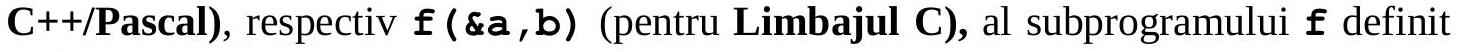
\includegraphics[max width=\textwidth]{2025_04_17_46e04c6acd873ea9558dg-080} mai jos.

\begin{verbatim}
Limbajul C++
int a,b;
void f(int&x,int y)
{ int b,c;
a++; b++; x=x*2; y=y*3;
b=x; c=y; c++; }
Limbajul C
int a,b;
void f(int*x,int y)
{ int b,c;
\end{verbatim}

\begin{verbatim}
Limbajul Pascal
var a,b:integer;
procedure f(var x:integer;
y:integer);
var b,c:integer;
begin
    inc(a); inc(b);
    x:=x*2; y:=y*3;
        b:=x; c:=y; inc(c) ;
end;
\end{verbatim}

\begin{verbatim}
    a++; b++; *x=*x*2;
y=y*3; b=*x; c=y; c++; }
\end{verbatim}

a) $\begin{aligned} & \text { Eroare de } \\ & \text { compilare }\end{aligned}$\\
b) 20\\
c) 22\\
d) 23\\
e) 11\\
f) 10\\
15. Se consideră subprogramul $f$ definit mai jos. Precizați ce valoare va avea $f(20,2)$.

\begin{verbatim}
Limbajul C++/C
int f(int x,int y)
{int p=1;
    if(x>1)
    { while(x%y==0)
            { p=p*y; x=x/y; }
if(p!=1)
return p+f(x,y+1);
    else return f(x,y+1);
            }
        else return 0;
}
\end{verbatim}

a) 9\\
b) 4\\
c) 10

\begin{verbatim}
Limbajul Pascal
function
$\mathrm{f}(\mathrm{x}, \mathrm{y}$ :integer) : integer;
var p :integer;
begin
    $\mathrm{p}:=1$;
if $x>1$ then
begin
    while $x \bmod y=0$ do
    begin
            p:=p*y; $x:=x \operatorname{div} y ; ~ e n d ;$
        if $\mathrm{p}<>1$ then $\mathrm{f}:=\mathrm{p}+\mathrm{f}(\mathrm{x}, \mathrm{y}+1)$
                else $\mathrm{f}:=\mathrm{f}(\mathrm{x}, \mathrm{y}+1)$;
            end
    else f:=0; end;
\end{verbatim}

d) 7\\
e) 11\\
f) 5

\section*{Varianta 16}
\begin{enumerate}
  \item Se consideră variabilele de tip întreg $a=15, b=30, c=5, d=10$ și $R$, indicați valoarea variabilei $R$ în urma executării instrucțiunii:\\
Limbajul C/C++ R=a+b/c+d; Limbajul Pascal R:=a + b div c + d;\\
a) 19\\
b) 17\\
c) 3\\
d) 31\\
e) 20\\
f) 15
  \item Fie următoarele două secvențe de cod:
\end{enumerate}

\section*{Limbajul C/C++}
Secvența 1:

\begin{verbatim}
s=0;
for(i=1;i<=n;i++)
    s=s+i*i;
\end{verbatim}

Secvența 2:

\begin{verbatim}
s=0; i=<initial>;
do
{s=s+i*i;
<instrucțiune>
} while(i>=1);
\end{verbatim}

\section*{Limbajul Pascal}
Secvența 1:

\begin{verbatim}
s:=0;
for i:=1 to n do
    s:=s+i*i;
\end{verbatim}

Secvența 2:

\begin{verbatim}
s:=O; i:=<initial>;
repeat
s:=s+i*i;
<instrucțiune>
until i=0;
\end{verbatim}

Indicați cu ce trebuie înlocuite <initial> și <instrucțiune> astfel încât cele două secvențe de cod să fie echivalente (în final variabila s să aibă aceeași valoare).

Limbajul C/C++\\
a) $n$ și i=i-1;\\
b) 1 și i=i+1;\\
c) n și $i=i+1$;\\
d) 0 și i=i+1;\\
e) $\mathrm{n}+1$ și i=i+1;\\
f) 0 și i=i-1;

Limbajul Pascal\\
a) n și i:=i-1;\\
b) 1 și i:=i+1;\\
c) n și $\mathrm{i}:=\mathrm{i}+1$;\\
d) 0 și i:=i+1;\\
e) n+1 și i:=i+1;\\
f) 0 și i:=i-1;\\
3. Precizați secvența de instrucțiuni echivalentă cu următoarea secvență de cod.

\begin{verbatim}
Limbajul C/C++
if (a>b)
    if(a%2==0)
        if(b%2==0) c=a;
    else c=b;
\end{verbatim}

Limbajul C/C++\\
a) if(a>b \&\& a\%2\hl{0 \&\& b\%2}0) c=a; if $(a>b) \& \& a \% 2==0 \quad \& \&$ $b \% 2!=0$ ) $c=b$;\\
b) if(a>b \&\& a\%2==0 \&\& $b \% 2==0$ ) $c=a$;

\begin{verbatim}
Limbajul Pascal
if a>b then
    if a mod 2=0 then
        if b mod 2=0 then c:=a
        else c:=b;
\end{verbatim}

Limbajul Pascal

\begin{verbatim}
a) if (a>b) and (a mod 2=0)
    and (b mod 2=0) then c:=a;
    if (a>b) and (a mod 2=0)
    and (b mod 2<>0) then c:=b;
\end{verbatim}

b) if $(a>b)$ and $(a \bmod 2=0)$\\
and ( $b \bmod 2=0$ ) then $c:=a$\\
else c:=b;

\begin{verbatim}
        else c=b;
c) if(a>b && a%2==0 &&
    b%2==0) c=a;
    if(a<b && a%2!=0 &&
    b%2!=0) c=b;
d) if(a>b && a%2==0 &&
    b%2==0) c=a;
    if(a<=b && a%2!=0 &&
    b%2!=0) c=b;
e) if(a>b && a%2==0 &&
    b%2==0) c=a;
f) if(a<=b && a%2!=0 &&
    b%2!=0) c=b;
\end{verbatim}

\begin{verbatim}
c) if (a>b) and (a mod 2=0)
    and (b mod 2=0) then c:=a;
    if (a<b) and (a mod 2<>0)
    and (b mod 2<>0) then c:=b;
\end{verbatim}

d) if $(a>b)$ and ( $a \bmod 2=0)$\\
and ( $b \bmod 2=0$ ) then $c:=a$;\\
if $(a<=b)$ and (a mod $2<>0$ )\\
and $(\mathrm{b}$ mod $2<>0)$ then $\mathrm{c}:=\mathrm{b}$;\\
e) if (a>b) and (a mod 2=0)\\
and (b mod 2=0) then $c:=a ;$\\
f) if $(a<=b)$ and $(a \bmod 2<>0)$\\
and $(b \bmod 2<>0)$ then $c:=b$;\\
4. Indicați numărul minim de muchii ce trebuie eliminate dintr-un graf neorientat complet care are 88 noduri astfel încât acesta să devină eulerian.\\
a) 0\\
b) 84\\
c) 88\\
d) 176\\
e) 10\\
f) 44\\
5. Precizați descendenții nodului 5 din arborele dat de următorul vector tați $(5,8,4,0,4,5,3,6,7,8)$.\\
a) $1,2,6,8,10$\\
b) $\mathbf{1}$ și $\mathbf{6}$\\
c) 4\\
d) $\mathbf{1 , 6}$, 7\\
e) $\mathbf{1}$ și $\mathbf{7}$\\
f) $\mathbf{6 s ̦ i} \mathbf{7}$\\
6. Se consideră un tablou bidimensional A, cu n linii şi $\mathbf{n}$ coloane, notăm cu Aij elementul aflat pe linia $i$ și coloana $j(1 \leq i \leq n, 1 \leq j \leq n)$. Precizați condiția necesară ca elementul Aij să fie situat pe prima diagonală de sub diagonala secundară, care este paralelă cu aceasta.\\
a) $i+j==n-1(C / C++)$ $i+j=n-1$ (Pascal)\\
b) $i+j==n+1$ (C/C++) $i+j=n+1$ (Pascal)\\
c) $i+j==n+2(C / C++)$ $i+j=n+2$ (Pascal)\\
d) $i==j+1(\mathrm{C} / \mathrm{C}++)$\\
e) $i==j(C / C++)$\\
f) $i+j==n-2(C / C++)$\\
$i=j+1$ (Pascal)\\
$i=j$ (Pascal)\\
$i+j=n-2$ (Pascal)\\
7. Precizați intervalul căruia îi aparţine valoarea memorată de variabila reală $\mathbf{x}$, astfel încât expresia următoare să aibă valoarea 1 (pentru Limbajul C/C++), true (pentru Limbajul Pascal)

\begin{verbatim}
Limbajul C/C++ $x<-10$ || ! (! ( $x>=10$ ) || $x>=100$ )
\end{verbatim}

\begin{verbatim}
Limbajul Pascal
(x<-10) or not(not(x>=10) or
(x>=100))
\end{verbatim}

a) $x \in(-\infty,-10) \cup[10,100)$\\
b) $x \in(-\infty,-10] \cup[10,100)$\\
c) $\mathbf{x} \in(-\infty,-\mathbf{1 0}) \cup(\mathbf{1 0}, \mathbf{1 0 0})$\\
d) $x \in(-\infty,-10) \cup[10,100]$\\
e) $x \in(-10,10) \cup(100,+\infty)$\\
f) $x \in(-10,100)$\\
8. În secvenţa de mai jos, variabilele $\mathbf{i}, \mathbf{j}, \mathbf{x}$ şi $\mathbf{y}$ sunt de tip întreg, iar variabila a memorează un tablou bidimensional în care prima linie şi prima coloană sunt numerotate cu 1. Toate elementele tabloului primesc valori în urma executării secvenței. Precizați care este valoarea elementului a [4] [4] (pentru limbajul C/C++), respectiv a [4,4] (pentru limbajul Pascal) în urma executării secvenței de mai jos.

\begin{verbatim}
Limbajul C/C++
x =3478;
for(j=4;j>=1;j--)
{ y=x;
    for(i=4;i>=1;i--)
    {
if(j%2==0)a[i][j]=10-y%10;
else a[i][j]=y%10;
y=y/10;
    }
x++;}
\end{verbatim}

a) 7\\
b) 3\\
c) 6\\
d) 4\\
e) 2\\
f) 8

\begin{verbatim}
Limbajul Pascal
x:=3478;
for j:=4 downto 1 do
begin
    y:=x;
    for i:=4 downto 1 do
    begin
        if $j \bmod 2=0$ then
            $a[i, j]:=10-y \bmod 10$
        else a[i,j]:=y mod 10;
        $\mathrm{y}:=\mathrm{y}$ div 10 ;end;
$x:=x+1$; end;
\end{verbatim}

\begin{enumerate}
  \setcounter{enumi}{8}
  \item Precizați numărul maxim de noduri izolate pe care le poate avea un graf neorientat cu 30 de noduri și 20 de muchii\\
a) 24\\
b) 23\\
c) 15\\
d) 25\\
e) 0\\
f) 10
  \item Se consideră un graf neorientat cu 9 noduri, al cărui vector de muchii este $\mathbf{M}=\{(\mathbf{1}, \mathbf{2})$, $(1,9),(2,3),(3,4),(3,7),(3,8),(4,5),(5,6),(5,7),(6,7),(6,8),(8,9)\}$. Indicați numărul minim de muchii care trebuie eliminate astfel încât graful să devină eulerian, dar să rămână hamiltonian.\\
a) 4\\
b) 0\\
c) Nu se poate\\
d) 2 e) 7\\
f) 3
  \item Se utilizează metoda backtracking pentru a genera șiruri de câte 5 caractere distincte din mulţimea $\{\mathrm{a}, \mathbf{1}, \mathrm{b}, \mathbf{2}, \mathrm{c}, \mathbf{3}, \mathrm{d}, \mathbf{4}\}$ cu proprietatea că nu poate să aibă două cifre sau două litere alăturate. Ştiind că primul șir generat este a1b2c, iar al doilea este a1b2d, precizați șirul obţinut imediat înainte de 2c4a1.\\
a) 2 c 3 d 4\\
b) 2 c 1 b 4\\
c) 2 b 4 d 3\\
d) $2 c 3 a 4$\\
e) 1 c 3 a 4\\
f) 2 c 1 a 4
  \item Indicați valoarea variabilei a la finalul executării secvenței următoare de program.
\end{enumerate}

\begin{verbatim}
Limbajul C/C++
char a[]="15iunie1970";
char v[]="aeiouAEIOUn";
int i;
for(i=0;i<strlen(a);i++) a:='15iunie1970';
Limbajul Pascal
var a,v:string;
    i:integer;
...
\end{verbatim}

\begin{verbatim}
if(a[i]>='O' && a[i]<='9')
    a[i]=v[a[i]-'0'];
\end{verbatim}

\begin{verbatim}
v:='aeiouAEIOUn';
for i:=1 to length(a) do
if (a[i]>='0') and (a[i]<='9')
then
a[i]:=v[ORD(a[i])-ORD('0') +1];
\end{verbatim}

a) Eroare de\\
b) iEiunieinOe\\
c) eAiunieeUIa\\
d) 152410211970\\
e) EiunieinO\\
f) AiunieeUI\\
13. Se consideră un tablou unidimensional a cu n numere naturale. Dacă pentru n se citește valoarea 7, iar a primește valorile: 7,4,8,2,9,6 și 2, precizați ce se va afișa la sfârșitul executării secvenței următoare de program.

\begin{verbatim}
Limbajul C++
int a[15],i,n,j;
cin>>n;
for(i=0;i<n;i++)
        cin>>a[i];
for(i=0;i<n;i++)
        if(a[i]%2==0)
{
    for(j=i;j<n-1;j++)
            a[j]=a[j+1];
    n--;
}
for(i=0;i<n;i++)
cout<<a[i]<<" ";
\end{verbatim}

\begin{verbatim}
Limbajul Pascal
var a:array[1..20] of
integer;
        i,j,n,k:integer;
read(n);
for i:=1 to n do read(a[i]);
i:=1;
while i<=n do
    begin
        if a[i] mod 2=0 then
            begin
                k:=n-1;
                for j:=i to k do
a[j]:=a[j+1];
            n:=n-1; end;
        i:=i+1; end;
for i:=1 to n do
write(a[i],' ');
\end{verbatim}

\section*{Limbajul C}
\begin{verbatim}
int a[15],i,n,j;
scanf("%d",&n);
for(i=0;i<n;i++)
    scanf("%d",&a[i]);
for(i=0;i<n;i++)
        if(a[i]%2==0)
{
    for(j=i;j<n-1;j++)
            a[j]=a[j+1];
    n--;
}
for(i=0;i<n;i++)
printf("%d ",a[i]);
\end{verbatim}

a) 7292\\
b) 79\\
c) $\mathbf{7 8 9 2}$\\
d) $\mathbf{7 4 2 9 6}$\\
e) 426\\
f) $\mathbf{4 8 2 6}$\\
14. Indicați valorile variabilelor $\mathbf{a}$ și $b$, în urma apelului $f(a, b, b)$ (pentru Limbajul C++/Pascal), respectiv $f(\& a, b, b)$ (pentru Limbajul C), al subprogramului $f$ definit mai jos.

\begin{verbatim}
Limbajul C++
int a,b;
void f(int&x,int y,int b)
{ a++; b++;
    x=x*2; y=y*3;
}
Limbajul C
int a,b;
void f(int*x,int y,int b)
{ a++; b++;
    *x=*x*2; y=y*3;
}
\end{verbatim}

a) Eroare de compilare\\
b) 23\\
c) 11\\
d) 20\\
e) 22\\
f) 10\\
15. Se consideră subprogramul $\mathbf{f}$ definit mai jos. Precizații ce valoare va avea $\mathrm{f}(1234,6789,1)$.

\begin{verbatim}
Limbajul C++/C
int f(int x,int y, int p)
{
if(y!=0)
    if( }\textrm{y}%2==0
        return
y%10*p+f(x/10,y/10,p*10);
    else
        return
x%10*p+f(x/10,y/10,p*10);
            else return 0;
}
\end{verbatim}

a) 1739\\
b) $\mathbf{4 8 6 2}$\\
c) 6789\\
d) 200\\
e) 6284\\
f) 1234

\begin{verbatim}
Limbajul Pascal
var a,b:integer;
procedure f(var x:integer;
y,b:integer) ;
begin
    inc(a); inc(b);
    x:=x*2; y:=y*3;
end;
\end{verbatim}

\begin{verbatim}
Limbajul Pascal
function
f(x,y,p:integer):integer;
begin
    if y<>0 then
        if y mod 2=0 then
            f:= y mod 10 * p +
f(x div 10,y div 10,p*10)
        else f:=x mod 10 * p +
    f(x div 10,y div 10,p*10)
    else f:=0;
end;
\end{verbatim}

\section*{Varianta 17}
\begin{enumerate}
  \item Alegeți secvențele de instrucțiuni prin care variabilei întregi pc i se atribuie valoarea primei cifre a unui număr natural dat prin variabila a.
\end{enumerate}

\begin{verbatim}
Limbajul C++
    pc=a/10;
    pc=a;while(pc>9)pc=pc/10;
    pc=a%10;
    pc=a;while (pc>9) pc=pc%10;
    pc=a;while (pc>0) pc=pc/10;
    pc=a;while (pc>0) pc=pc%10;
\end{verbatim}

\section*{Limbajul C}
\begin{verbatim}
pc=a/10;
pc=a;while(pc>9) pc=pc/10;
pc=a%10;
pc=a;while (pc>9) pc=pc%10;
pc=a;while (pc>0) pc=pc%10;
pc=a;while(pc>0) pc=pc/10;
\end{verbatim}

\begin{verbatim}
Limbajul Pascal
1. pc:=a div 10;
2. pc:=a; while (pc>9)
    do pc:=pc div 10;
3. pc:=a mod 10;
4. pc:=a; while (pc>9)
    do pc:=pc mod 10;
5. pc:=a; while (pc>0)
    do pc:=pc div 10;
6. pc:=a; while (pc>0)
    do pc:=pc mod 10;
\end{verbatim}

a) 1\\
b) 2\\
c) 3\\
d) 4\\
e) 5\\
f) 6\\
2. Precizați care dintre următoarele secvențe de instrucțiuni atribuie variabilei întregi $p$, valoarea $3^{\text {n }}$, unde variabila $n$ reprezintă un număr natural dat.

\begin{verbatim}
Limbajul C++
    p=1;for(i=1;i<=n;i++)p*=n;
    p=3;for(i=1;i<=n;i++) p*=i;
    p=1;i=0;while(i<n)p*=3;i++;
    p=1;for(i=1;i<=n;i++)p*=3;
    p=3;for(i=n;i>=0;i--)p*=3;
    p=1;for(i=n;i>=0;i--)p*=3;
\end{verbatim}

\section*{Limbajul C}
\begin{verbatim}
p=1;for(i=1;i<=n;i++) p*=n;
p=3;for(i=1;i<=n;i++) p*=i;
p=1;i=0;while (i<n) p*=3;i++;
p=1;for(i=1;i<=n;i++) p*=3;
p=3;for(i=n;i>=0;i--) p*=3;
p=1;for(i=n;i>=0;i--) p*=3;
\end{verbatim}

Limbajul Pascal

\begin{verbatim}
1. p:=1;for i:=1 to n
    do p:=p*n;
2. p:=3;for i:=1 to n
    do p:=p*i;
3. p:=1; i:=0;
    while (i<n) do
    p:=p*3; inc(i);
4. p:=1;for i:=1 to n
    do p:=p*3;
5. p:=3;
    for i:=n downto O do
    p:=p*3;
6. p:=1;
    for i:=n downto O do
    p:=p*3;
\end{verbatim}

a) 1\\
b) 2\\
c) 3\\
d) 4\\
e) 5\\
f) 6\\
3. Indicați valoarea returnată de funcția definită mai jos, la apelul sp (3).

\begin{verbatim}
Limbajul C
int sp(int n)
{
if(n>1)
    return
sp(n-1)+n*(n+1)*(n+2);
    else return 6;}
\end{verbatim}

Limbajul C++\\
int $s p($ int $n$ )\\
\{if( $\mathrm{n}>1$ ) return\\
$\mathrm{sp}(\mathrm{n}-1)+\mathrm{n}$ * $(\mathrm{n}+1)$ * $(\mathrm{n}+2)$;\\
else return 6;\}\\
a) 30\\
b) 60\\
c) 90\\
d) 120\\
e) 150\\
e) 150\\
f) 180\\
4. Indicați expresia corectă din punct de vedere sintactic și care are ca valoare $\mathbf{3}^{2020}$.

\section*{Limbajul C++}
\begin{verbatim}
$\exp (2020 * \log (3))$
$\exp (\log (2020))$ *exp (3)
$\log (3)$ *exp (2020)
$\log (3 * \exp (2020))$
$\exp (\log (2020) * \log (3))$
\end{verbatim}

\begin{enumerate}
  \setcounter{enumi}{5}
  \item $\log (\exp (2020 * \log (3)))$
\end{enumerate}

\section*{Limbajul C}
\begin{verbatim}
$\exp (2020 * \log (3))$
$\exp (\log (2020)) * \exp (3)$
$\log (3) * \exp (2020)$
log (3*exp (2020))
$\exp (\log (2020) * \log (3))$
\end{verbatim}

\begin{enumerate}
  \setcounter{enumi}{5}
  \item $\log (\exp (2020 * \log (3)))$\\
a) 1\\
b) 2\\
c) 3\\
d) 4\\
e) 5\\
f) 6
  \item Fie graful neorientat $\mathbf{G}=(\mathrm{V}, \mathbf{M})$, unde V este mulțimea nodurilor grafului, $\operatorname{card}(\mathrm{V})=\mathrm{n}$, respectiv, M este mulțimea muchiilor grafului, iar $\operatorname{card}(\mathrm{M})=\mathrm{m}$. Graful dat are $p$ componente conexe. Dacă $\mathrm{n}=1010, \mathrm{~m}=2020$ iar $\mathrm{p}=100$, precizați care este numărul maximal de cicluri independente care pot fi construite concomitent pe graf. Prin cicluri independente se înțelege, cicluri care conțin cel puţin câte o muchie care aparține doar unuia din ele.\\
a) 1001\\
b) 1010\\
c) 1011\\
d) 1100\\
e) 1101\\
f) 1110
  \item Indicați valoarea variabilei text după executarea instrucţiunilor de mai jos.
\end{enumerate}

Limbajul Pascal

\begin{verbatim}
exp (2020*ln(3))
exp(ln(2020))*exp (3)
ln(3)*exp (2020)
ln(3*exp (2020))
exp(log(2020)*ln(3))
log(exp(2020*ln(3)))
\end{verbatim}

\begin{verbatim}
Limbajul Pascal
function
sp(n:integer) :integer;
Begin
if(n>1) then
    sp:=sp(n-1)+n*(n+1)*(n+2)
        else
            sp:=6;
End;
\end{verbatim}

\begin{verbatim}
Limbajul C++
char text[250];
strncpy(text,
strstr("Admitere Poli 2020",
"oli"),9);
text[9]='\0';
Limbajul C
char text[250];
strncpy(text,
strstr("Admitere Poli 2020",
"oli"),9);
text[9]='\0';
\end{verbatim}

\begin{verbatim}
Limbajul Pascal
var
text:string[250];p:integer;
Begin
text:='Admitere Poli 2020';
p:=pos('oli',text);
text:=copy(text,p,9);
End.
\end{verbatim}

a) Admitere\\
b) Admitere 2020\\
c) Admitere Poli\\
d) Poli 2020\\
e) oli 2020\\
f) 2020\\
7. Indicați valoarea variabilei text după executarea secvenței de instrucţiuni de mai jos.

\begin{verbatim}
Limbajul C++
char text[250];
strcpy(text,strstr("Admitere Politehnica Bucuresti
2020", "Poli")+strlen("240820201731"));
cout<<strcat(text," ADMIS");
Limbajul C
char text[250];
strcpy(text,strstr("Admitere Politehnica Bucuresti
2020", "Poli")+strlen("240820201731"));
printf(" %s \n", strcat(text," ADMIS"));
Limbajul Pascal
var text:string[250];p:integer;
Begin
text:='Admitere Politehnica Bucuresti 2020';
p:=pos('Poli',text);
text:=copy(text,p+length('240820201731'),length(text));
text:=concat(text,' ADMIS'); writeln(text); End.
\end{verbatim}

a) Admitere 2020 ADMIS\\
b) Admitere 2020\\
c) Bucuresti ADMIS\\
d) Bucuresti 2020 ADMIS\\
e) Politehnica ADMIS\\
f) Politehnica 2020 ADMIS\\
8. Utilizând metoda backtracking, se generează toate modalitățile de a se îmbrăca un inginer. Ș̦tiind că el are la dispoziție 12 cămăși, 8 pantaloni și 9 cravate, indicați numărul de modalități de a se îmbrăca, folosind toate cele trei elemente vestimentare, pe care le are inginerul.\\
a) 864\\
b) 204\\
c) 168\\
d) 108\\
e) 96\\
f) 29\\
9. Precizați care este cea mai mare valoare pe care o poate lua variabila întreagă $\mathbf{n}$ astfel încât să se afișeze mesajul Corect.

\begin{verbatim}
Limbajul C
if(n<17-3*n)
    printf("Corect");
else
printf("Incorect");
\end{verbatim}

\begin{verbatim}
Limbajul C++
if (n<17-3*n)
cout<<"Corect";
else
cout<<"Incorect";
\end{verbatim}

\begin{verbatim}
Limbajul Pascal
if n<17-3*n then
write("Corect")
else
write("Incorect");
\end{verbatim}

a) 17\\
b) 15\\
c) 12\\
d) 10\\
e) 7\\
f) 4\\
10. Precizați care este valoarea inițială a variabilei întregi $n$ pentru ca secvența de program de mai jos să afișeze $\mathbf{\$} \mathbf{\$} \mathbf{\$} \mathbf{\$}$.

\begin{verbatim}
Limbajul C
while(n!=3)
    { n--;
        printf("$$");}
\end{verbatim}

a) 1\\
b) 2\\
c) 3\\
d) 3\\
e) 5 f) nici $\mathbf{o}$ valoare

\begin{verbatim}
Limbajul Pascal
while n<>3 do
begin
dec(n);
write('$$');end;
\end{verbatim}

\begin{enumerate}
  \setcounter{enumi}{10}
  \item Se construiește un tablou bidimensional cu $n$ linii și n coloane, în variabila $\mathbf{A}$ prin secvența de mai jos, unde variabila $n$ este un număr natural nenul dat.
\end{enumerate}

\begin{verbatim}
Limbajul C
for(i=1;i<=n;i++)
for(j=1;j<=n;j++)
A[i][j]=(2*i+j)/2;
\end{verbatim}

\begin{verbatim}
Limbajul C++
while(n!=3)
    { n--;
    cout<<"$$";}
\end{verbatim}

\begin{verbatim}
Limbajul C++
for(i=1;i<=n;i++)
for( }\textrm{j}=1;\textrm{j}<=n;j++
A[i][j]=(2*i+j)/2;
\end{verbatim}

Limbajul Pascal for $\mathrm{i}:=1$ to n do for $i:=1$ to $n$ do A[i,j]:=(2*i+j)/2;

Precizați suma elementelor alfate pe diagonala principală a tabloului bidimensional A, în urma execuției secvenței de mai sus.\\
a) $\frac{3}{4} \cdot(n+1) \cdot n$\\
b) $\frac{3}{4} \cdot n^{2}$\\
c) $\frac{4}{3} \cdot n^{2}$\\
d) $\frac{1}{4} \cdot(n+1) \cdot n$\\
e) $\frac{1}{4} \cdot n^{2}$\\
f) $\frac{1}{3} \cdot n^{2}$\\
12. Se consideră declarările de mai jos. Indicați tipul expresiei aa.a.a

\begin{center}
\begin{tabular}{|l|l|l|}
\hline
Limbajul C struct S1 \{int a; char b;\}; struct S2 \{float a; double b; \}; struct S3 \{struct S1 a; struct S2 b; \} $a \mathrm{a}, \mathrm{bb}$; & Limbajul C++ struct S1 \{int a; char b;\}; struct S2 \{float a; double b; \}; struct S3 \{struct S1 a; struct S2 b; \} $a \mathrm{a}, \mathrm{bb}$; & Limbajul Pascal Type S1=Record a: integer; b: char; End; S2=Record a: real; b: real; End; S3=Record a: S1; b: S2; End; var aa,bb:S3; \\
\hline
\end{tabular}
\end{center}

a) long/ long/ longint\\
b) float/ float/ real\\
c) int/ int/ integer\\
d) double/ double/ real\\
e) char/ char/char\\
f) nu putem avea în înregistrări diferite, câmpuri cu același nume\\
13. Stabiliți care este valoarea inițială a variabilei naturale i pentru ca secvența de program de mai jos să afișeze valorile $1 \begin{array}{llllll}1 & 2 & 4 & 5 & 6\end{array}$.

\begin{verbatim}
Limbajul C
k=1;
for(i=...i<=2020;i++)
{
    printf("%d ",k);
    k++;
}
\end{verbatim}

\begin{verbatim}
Limbajul C++
k=1;
for(i=...i<=2020;i++)
{
    cout<<k<<" ";
    k++;
}
\end{verbatim}

\begin{verbatim}
Limbajul Pascal
$\mathrm{k}:=1$;
for $i=$... to 2020 do
Begin
    Write(k,' ');
    inc (k);
end;
\end{verbatim}

a) 7\\
b) 17\\
c) 283\\
d) 314\\
e) 2013\\
f) 2014\\
14. Se consideră o mulțime A cu n numere naturale. Precizați care este complexitatea temporală pentru a genera toate submulțimile care au proprietatea că suma elementelor fiecărei submulțimi generate este divizibilă cu n.\\
a) $\mathbf{O}(\mathbf{n} \cdot \log (\mathrm{n}))$\\
b) $\mathbf{O}(\mathbf{n}+\log (\mathrm{n}))$\\
c) $\mathbf{O}\left(2^{\text {n }}\right)$\\
d) $\mathbf{O}\left(\mathbf{n}^{3}\right)$\\
e) $\mathbf{O}\left(\mathbf{n}^{2}\right)$\\
f) $\mathbf{O}(\mathbf{n})$\\
15. Precizați complexitatea timp pentru secvența de program de mai jos.

\begin{verbatim}
Limbajul C
k=0;
for(int a=n;a>=1;a/=2)
    for(int b=a;b>=1;b--)
        k++;
printf("%i \n",k);
Limbajul C++
k=0;
for(int a=n;a>=1;a/=2)
    for(int b=a;b>=1;b--)
        k++;
cout<<k;
\end{verbatim}

a) $\mathbf{O}(\mathbf{n} \cdot \log (\mathrm{n}))$\\
b) $\mathbf{O}(\mathrm{n}+\log (\mathrm{n}))$\\
c) $\mathbf{O}\left(\mathbf{2}^{\text {n }}\right)$\\
d) $\mathbf{O}\left(\mathbf{n}^{2}\right)$\\
e) $\mathbf{O}(\mathbf{n})$\\
f) $\mathbf{O}(1)$

\begin{verbatim}
Limbajul Pascal
k:=0;a:=n;
while(a>=1) do
begin
    b:=a;
        while(b>=1) do
            begin
                k++;
                dec (b) ;
            end;
    a:=a div 2;
end;
write(k);
\end{verbatim}

\section*{Varianta 18}
\begin{enumerate}
  \item Precizați care dintre următoarele secvențe de instrucțiuni atribuie variabilei întregi pc valoarea 100, unde $\mathbf{a}=559020$.
\end{enumerate}

\begin{verbatim}
Limbajul C
1. pc=a/100*a%10;
2. pc=a;while(pc>9) pc=pc/10;
    pc*=a%100;
3. pc=a%100;
4. pc=a;while(pc>9) pc:=pc%10;
    pc*=a%100;
5. pc=a/10;
    while(pc>0) pc=pc/10;
    pc*=a%100;
6. pc=a;while (pc>0) pc=pc/10;
    pc*=a%100;
Limbajul C++
    pc=a/100*a%10;
    pc=a;while (pc>9) pc=pc/10;
    pc*=a%100;
3. pc=a%100;
    pc=a;while(pc>9) pc=pc%10;
    pc*=a%100;
5. pc=a/10;
    while(pc>9) pc=pc/10;
    pc*=a%100;
6. pc=a;while(pc>0) pc=pc/10;
    pc*=a%100;
\end{verbatim}

a) 1\\
b) 2\\
c) 3\\
d) 4\\
e) 5\\
f) 6\\
2. Precizați care dintre următoarele secvențe de instrucțiuni de mai jos, atribuie variabilei întregi $\mathbf{p}$ valoarea împărțirii întregi a numărului $\mathbf{a}$ la numărul $\mathbf{b}$, unde variabilele $\mathbf{a}$ și $\mathbf{b}$ reprezintă două numere întregi date.

\begin{verbatim}
Limbajul C
    p=1;s=0;
    for(i=1;i<=b;i++)
    p-=b;s++;
2. p=a;
    for(i=1;i<=b;i++)p-=i;
3. p=1;i=0;
    while(i<b) p-=a;i++;
4. p=0;s=a;
\end{verbatim}

\begin{verbatim}
Limbajul Pascal
    pc:=a div 10 * a mod 10;
2. pc:=a;
    while (pc>9) do
        pc:=pc div 10;
    pc:=pc*(a mod 100);
    pc:=a mod 100;
4. pc:=a;
    while (pc>9) do
        pc:=pc mod 10;
    pc:=pc*(a mod 100);
5. pc:=a/10;
    while (pc>0) do
            pc:=pc div 10;
    pc:=pc*(a mod 100);
6. pc:=a;
    while (pc>0) do
        pc:=pc div 10;
    pc:=pc*(a mod 100);
\end{verbatim}

\section*{Limbajul Pascal}
\begin{enumerate}
  \item $p:=1 ; s:=0$;for $i:=1$ to $b$ do $p:=p-n$;inc (s);
  \item $p:=a ; f o r ~ i:=1$ to $b$ do p:=p-i;
  \item $p:=1 ; i:=0$; while i<b do p:=p*a;inc(i);
  \item $\mathrm{p}:=0$;s:=a;while (s>0)
\end{enumerate}

\begin{verbatim}
for(i=1;i<=b&&s>0;i++)
{p++;s-=b;}
5. p=a;
for(i=0;i<=b;i++)p-=b;
6. p=1;
for(i=0;i<=b;i++)p-=b;
\end{verbatim}

Limbajul C++

\begin{verbatim}
1. p=1;s=0;
    for(i=1;i<=b;i++)
    p-=b;s++;
\end{verbatim}

\begin{enumerate}
  \setcounter{enumi}{1}
  \item $\mathrm{p}=\mathrm{a}$;\\
for (i=1;i<=b;i++)p-=i;
  \item $p=1$; $i=0$; while ( $i<b) p-=a$;\\
i++;
  \item $\mathrm{p}=0$; $\mathrm{s}=\mathrm{a}$;\\
for (i=1;i<=b\&\&s>0;i++)\\
\{p++;s-=b; \}
  \item $\mathrm{p}=\mathrm{a}$;\\
for (i=0;i<=b;i++)p-=b;
  \item $\mathrm{p}=1$;\\
for (i=0; i<=b;i++)p-=b;\\
a) 1\\
b) 2\\
c) 3\\
d) 4\\
e) 5\\
f) 6
  \item Precizați care este valoarea returnată de funcția definită mai jos, la apelul sp (5).
\end{enumerate}

\begin{verbatim}
Limbajul C++
float sp(int n)
{if(n>1)
return sp (n-1)+1./(n* (n+1));
    else return 0.5;}
Limbajul C
float sp(int n)
{if(n>1)
return sp (n-1)+1./(n* (n+1));
    else return 0.5;}
\end{verbatim}

\begin{enumerate}
  \setcounter{enumi}{3}
  \item Precizați care dintre următoarele expresii de mai jos reprezintă valoare polinomului sunt introduse de la tastatură.
\end{enumerate}

Limbajul C

\begin{verbatim}
1. p=0; for (k=0;k<=n;k++)
        p=p+(n-k) *pow (x,k) ;
2. p=1; for (k=0;k<=n;k++)
\end{verbatim}

a) 0.83\\
b) 0.82\\
c) 0.81\\
d) 0.38\\
d) 0.38\\
e) 0.28\\
e) 0.28\\
f) 0.18 $p=\sum_{k=0}^{n}(n-k) \cdot X^{k}$, pentru un număr $\mathbf{x}$ real pozitiv, iar $\mathbf{n}$ este un număr natural, $\mathbf{x}$ și $\mathbf{n}$

\begin{verbatim}
Limbajul Pascal
function
sp (n:integer) :real;
Begin
if(n>1) then
sp:=sp (n-1)+1/(n* (n+1))
    else
        sp:=0.5;
end;
\end{verbatim}

Limbajul Pascal

\begin{enumerate}
  \item $\mathrm{p}:=0$; for $\mathrm{k}:=0$ to n do $\mathrm{p}:=\mathrm{p}+(\mathrm{n}-\mathrm{k}) * \exp (\mathrm{k} * \ln (\mathrm{x}))$;
  \item $p:=1$; for $k:=0$ to $n$ do
\end{enumerate}

\begin{verbatim}
    p=p+(n-k) *pow (x,k);
3. p=1; for (k=0;k<n;k++)
    p=p+(n-k) *pow (x,k) ;
4. p=0; for (k=0;k<=n+1;k++)
        p=p+(n-k) *pow (x,k) ;
5. p=1; for (k=0;k<=n+1;k++)
    p=p+(n-k) *pow (x,k) ;
6. p=0;for (k=0;k<n;k++)
    p=p+(n-k) *pow (x,k) ;
\end{verbatim}

\begin{verbatim}
    p:=p+(n-k) * exp (k*ln(x));
3. p:=1;for k:=0 to n-1 do
    p:=p+(n-k) * exp (k*ln(x));
4. p:=0;for k:=0 to n+1 do
    p:=p+(n-k) * exp (k* ln (x));
5. p:=1;for k:=0 to n+1 do
    p:=p+(n-k) * exp (k*ln(x));
6. p:=0;for k:=0 to n-1 do
    p:=p+(n-k)*exp (k*ln(x));
\end{verbatim}

Limbajul C++

\begin{verbatim}
p=0;for (k=0;k<=n;k++)p=p+(n-k) *pow (x,k);
p=1 ; for (k=0;k<=n;k++) p=p+(n-k) *pow (x,k);
p=1;for (k=0;k<n;k++) p=p+(n-k) *pow (x,k) ;
p=0;for (k=0;k<=n+1;k++) p=p+(n-k) *pow (x,k);
p=1;for (k=0;k<=n+1;k++) p=p+(n-k) *pow (x,k);
p=0;for (k=0;k<n;k++) p=p+(n-k) *pow (x,k);
\end{verbatim}

a) 1\\
b) 2\\
c) 3\\
d) 4\\
e) 5\\
f) 6\\
5. Fie graful neorientat $\mathrm{G}=(\mathrm{V}, \mathrm{M})$, unde V este mulțimea nodurilor grafului, $\operatorname{card}(\mathrm{V})=\mathrm{n}$, respectiv, $\mathbf{M}$ este mulțimea muchiilor grafului, $\operatorname{iar} \operatorname{card}(\mathbf{M})=\mathrm{m}$. Având la dispoziție cele n noduri se pot construi 32768 de grafuri neorintate distincte, precizați valoarea variabilei $n$.\\
a) 15\\
b) 14\\
c) 13\\
d) 8\\
e) 7\\
f) 6\\
6. Precizați care este valoare variabilei text după executarea instrucțiunilor de mai jos.

\begin{verbatim}
Limbajul C
char text[250]="";
strncpy(text,strstr("Admitere Poli 2020","Poli"),9);
text[9]='\0';
for(int k=strlen(text)-1;k>=0;k--) printf("%c",text[k]);
Limbajul C++
char text[250];
strncpy(text,strstr("Admitere Poli 2020","Poli"),9);
text[9]='\0';
for(int k=strlen(text)-1;k>=0;k--) cout<<text[k];
cout<<text;
Limbajul Pascal
var text:string[250];
c:char;
p,k:integer;
Begin
text:='Admitere Poli 2020'; p:=pos('Poli',text);
\end{verbatim}

\begin{verbatim}
text:=copy(text, p,length(text)) ;
for k:=1 to length(text) div 2 do
    begin
        c:=text[k]; text[k]:=text[length(text) -k+1];
        text[length(text) -k+1]:=c;
    end;
writeln(text);
End.
\end{verbatim}

a) Poli 2020\\
b) oli 2020\\
c) Admitere Poli\\
d) 0202 iloP eretimdA\\
e) 0202 eretimdA\\
f) 0202 iloP\\
7. Precizați ce valoare are variabila text după executarea instrucţiunii de mai jos.

\begin{verbatim}
Limbajul C
char text[250], nou[250];
strcpy(text,strstr("Admitere Politehnica Bucuresti 2020",
"ere")+strlen("2408")) ;
strcpy(nou,text) ; strnset(nou,'X',12);
strncat(text,nou,12); printf("%s \n", text);
Limbajul C++
char text[250], nou[250];
strcpy(text,strstr("Admitere Politehnica Bucuresti 2020",
"ere")+strlen("2408")) ;
strcpy(nou,text) ; strnset(nou,'X',12);
strncat(text,nou,12); cout<<text;
Limbajul Pascal
var text:string[250];
c:char;
p,i:integer;
Begin
text:='Admitere Poli 2020'; p:=pos('Poli',text);
text:=copy(text, p,length (text)) ;
for i:=1 to length(text) div 2 do
begin
c:=text[i]; text[i]:=text[length(text)-i+1];
text[length(text)-i+1]:=c;
end;
writeln(text);
End.
\end{verbatim}

a) Bucuresti 2020 XXXXXX\\
b) Politehnica Bucuresti 2020XXXXXX\\
c) Politehnica 2020XXXXXXXXXX\\
d) Politehnica Bucuresti 2020XXXXXXXXXXXX\\
e) Bucuresti 2020 XXXXXXXXXXXX\\
f) Bucuresti 2020XXXXXX\\
8. Utilizând metoda backtracking, se generează toate modalitățile de a se forma o echipă de ingineri cu 5 membrii. Echipa trebuie să fie mixtă, formată din exact 2 ingineri și restul\\
inginere. Știind că instituția are 24 ingineri, iar inginere de 3 ori mai multe, care este numărul de echipe de ingineri care se pot forma?\\
a) 283946040\\
b) 283948060\\
c)283946080\\
d) 16832340\\
e) $\mathbf{1 6 8 3 2 3 8 0}$\\
f) $\mathbf{1 6 4 6 0 6 4 0}$\\
9. Fiind date două tablouri unidimensionale ordonate, fiecare cu n valori, se dorește obținerea unui al treilea tablou unidimensional ordonat, care va conține, toate elementele celor două tablouri în ordine descrescătoare. Algoritmul descris, efectuează în medie, nr comparații pentru a ordona elementele celor doi vectori. Numărul nr reprezintă complexitatea algoritmului de sortare și este:\\
a) $\mathbf{O}\left(\mathbf{n}^{2}\right)$\\
b) $\mathbf{O}\left(\mathbf{n}^{3}\right)$\\
c) $\mathbf{O}(\mathbf{n})$\\
d) $\mathbf{O}\left(\mathbf{n}^{2}+\mathbf{n}\right)$\\
e) $\mathbf{O}(\log (3) \cdot n)$\\
f) $\mathbf{O}(\log (2))$\\
10. Fie trei tije numerotate cu 1, $\mathbf{2}$ și $\mathbf{3}$. Problema constă în mutarea celor $\mathbf{n}$ discuri de pe tija 1, pe tija 2, prin intermediul tijei 3, cu următoarele restricții: la fiecare mutare se deplasează un singur disc; discurile se mută numai de pe o tijă pe alta; un disc cu diametru mai mare nu poate fi așezat peste un disc cu diametru mai mic. Pentru $n=1$, mutăm discul pe ultima tije. Pentru n=2, se fac mutările $1 \rightarrow 3,1 \rightarrow 2,3 \rightarrow 2$. În cazul în care n>3 problema se complică. Respectând restricțiile date se realizează un algoritm de rezolvare a problemei. Precizați complexitatea algoritmului de rezolvare al problemei prezentate.\\
a) $\theta\left(n \cdot \log 3\left(n^{3}\right)\right)$\\
b) $\theta\left(3^{n} \cdot \log 3(n)\right)$\\
c) $\theta\left(3^{n}\right)$\\
d) $\theta\left(2^{n}\right)$\\
e) $\theta\left(n^{2} \cdot \log \left(n^{2}\right)\right)$\\
f) $\theta\left(2^{n} \cdot \log \left(2^{n}\right)\right)$\\
11. Se construiește un tablou bidimensional cu $\mathbf{n} \times \mathbf{n}$ elemente, în variabila $\mathbf{A}$ prin secvența de mai jos, unde variabila $\mathbf{n}$ este un număr natural nenul dat de la tastatură.

\begin{verbatim}
Limbajul C
for (i=1;i<=n;i++)
for ( $\mathbf{j = 1 ; j < = n ; j + + )}$
A[i][j]=(3*i+2*j)/2;
\end{verbatim}

\begin{verbatim}
Limbajul C++
for (i=1;i<=n;i++)
for ( $\mathrm{j}=1$; $\mathrm{j}<=\mathrm{n} ; \mathrm{j}++$ )
A[i][j]=(3*i+2*j)/2;
\end{verbatim}

Limbajul Pascal\\
for $\mathrm{i}:=1$ to n do for $i:=1$ to $n$ do\\[0pt]
A[i,j]:=(3\textit{i+2}j)/2

Precizați care este suma elementelor de pe diagonala secundară a tabloului bidimensional A, în urma execuției secvenței de mai sus.\\
a) $\frac{5}{4} \cdot(n+1) \cdot n$\\
b) $\frac{3}{4} \cdot(n+1) \cdot n$\\
c) $\frac{5}{4} \cdot n^{2}$\\
d) $\frac{3}{4} \cdot n^{2}$\\
e) $\frac{3}{4} \cdot(n-1) \cdot n$\\
f) $\frac{5}{4} \cdot(n-1) \cdot n$\\
12. Se consideră declarările de mai jos. Precizați care este tipul expresiei bb.b.b.

\begin{verbatim}
Limbajul C
struct S1{ int a;char b;};
struct S2{ float a;double b;};
struct S3{struct S1 a;
        struct S2 b;} aa, bb;
Limbajul C++
struct S1{ int a;char b;};
struct S2{ float a;double b;};
struct S3{struct S1 a;
    struct S2 b;} aa, bb;
\end{verbatim}

\begin{verbatim}
Limbajul Pascal
Type S1=Record
        a: integer;
        b: char; End;
    S2=Record
        a: real;
        b: real;
    End;
    S3=Record
        a: S1;
        b: S2;
\end{verbatim}

\begin{verbatim}
    End;
var aa,bb:S3;
c) double/double/ real
f) nu putem avea în înregistrări diferite, câmpuri cu același nume
\end{verbatim}

a) long/ long/ longint\\
b) float/ float/ real\\
d) int/ int/ integer\\
e) char/ char/ char\\
13. Precizați care vor fi valorile afișate în urma rulării programului de mai jos pentru variabilele $\mathrm{a}=2020$, iar $\mathrm{b}=17$.

\begin{verbatim}
Limbajul C
#include<stdio.h>
    int a,b;
void f(int n,int m)
{
if(n!=m)
        if(n>m)
                f(n-m,m);
            else
            f(n,m-n);
else
    {printf("%i",a*b/n);
    printf("%i ",m);
    }
}
int main()
{scanf("%i ",&a);
    scanf("%i ",&b);
    f(a,b) ;
    return 0;
}
\end{verbatim}

a) $\mathbf{8 0 8 0} \mathbf{4}$\\
b) $\mathbf{6 0 6 0} 5$\\
c) $\mathbf{4 0 4 0} \mathbf{6}$ d) $\mathbf{2 0 2 0} 2020$\\
c) 40406\\
d) 20202020\\
e) 343401\\
f) 161442

\begin{verbatim}
Limbajul C++
#include<iostream>
using namespace
std;
    int a,b;
void f(int n,int m)
{
if(n!=m)
        if(n>m)
                    f(n-m,m);
                else
                    f(n,m-n);
            else
cout<<a*b/n<<"
"<<m;
}
int main()
{ cin>>a>>b;
        f(a,b);
return 0;
}
\end{verbatim}

\begin{verbatim}
Limbajul Pascal
var a,b:integer;
procedure
f(n,m:integer);
Begin
if n<>m then
    if n>m then
        f(n-m,m)
    else
        f(n,m-n)
else
    write(a*b div n,'
',m);
end;
begin
    readln(a,b);
    f(a,b);
end.
\end{verbatim}

\begin{enumerate}
  \setcounter{enumi}{13}
  \item Se consideră un graf neorientat conex cu noduri și m muchii, iar gradul fiecărui nod este par. Precizați care este complexitatea temporală pentru determinarea unui ciclu eulerian în acest graf pentru algoritmii care pornesc de la o parcurgere. Graful este reprezentat folosind liste de adiaceță.\\
a) $\mathbf{O}(\mathbf{n}+\mathbf{m})$\\
b) $\mathbf{O}(\mathrm{n})$\\
c) $\mathbf{O}(\mathbf{n} \cdot \mathbf{m})$\\
d) $\mathbf{O}(\mathrm{m})$\\
e) $\mathbf{O}(\mathrm{m} \cdot \log (2))$\\
f) $\mathbf{O}(\mathrm{n} \cdot \log (2))$
  \item Precizați complexitatea timp pentru secvența de program de mai jos.
\end{enumerate}

\begin{verbatim}
Limbajul C
k=0;
for(int a=n;a>=1;a--)
    for(int b=n;b>=1;b--)
        k++;
printf("%i \n",k);
\end{verbatim}

\begin{verbatim}
Limbajul Pascal
k:=0;
a:=n;
while(a>=1) do
begin
    b:=n;
| Limbajul Pascal
\end{verbatim}

muchii, iar gra\\
O(m•log(2)) $\mathbf{1}$ f) $\mathbf{1 6 1 4 4} 2$\\
gradul fiecărui nod\\
minarea unui ciclu\\
urgere. Graful este\\
f) $\mathbf{O}(\mathbf{n} \cdot \log (\mathbf{2}))$\\
$a:=n ;$\\
while $(a>=1)$ do\\
begin\\
$b:$

\begin{verbatim}
Limbajul C++
k=0;
for(int a=n;a>=1;a--)
    for(int b=n;b>=1;b--)
        k++;
cout<<k;
\end{verbatim}

a) $O(n \cdot \log n)$\\
b) $0\left(2^{n}\right)$\\
c) $O\left(n^{3}\right)$

\begin{verbatim}
while(b>=1) do
        begin
        k++;
        dec (b) ;
    end;
    dec(a);
end;
write(k) ;
\end{verbatim}

d) $O\left(n^{2}\right)$\\
e) $\mathrm{O}(\mathrm{n})$\\
f) O (1)

\section*{Varianta 19}
\begin{enumerate}
  \item Ce se va afișa în urma rulării secvenței de cod de mai jos:
\end{enumerate}

\begin{verbatim}
Limbajul C++
int main() {
    int p, *q; p = 45; q = &p;
cout << q[0];
}
\end{verbatim}

Limbajul C\\
int main() \{\\
int $\mathrm{p}, * \mathrm{q} ; \mathrm{p}=45 ; \mathrm{q}=\mathrm{q} \mathrm{p}$;\\[0pt]
printf("\%d", q[0]);\\
\}\\
a) 100\\
b) 45\\
c) Eroare\\
d) 0\\
e) 43\\
f) 1\\
2. Fie secvența de cod următoare, în care se consideră că variabilele $\mathbf{a}, \mathrm{i}, \mathrm{n}$ rețin numere întregi:

\begin{verbatim}
Limbajul C++
cin>>n; a = 1; i = 2;
while(i<n && a>0){
        if(n%i == 0) a=0;
            else
            i++; cout<<i;}
Limbajul C
scanf("%d",&n); a = 1; i = 2;
while (i<n && a>0) {
    if(n%i == 0) a = 0;
    else i++; printf("%d",i);}
\end{verbatim}

\begin{verbatim}
Limbajul Pascal
var p:integer; q:^integer;
begin
        p := 45; q := @p;
        write(q^);
end.
\end{verbatim}

\begin{verbatim}
Limbajul Pascal
read(n);
a := 1; i := 2;
while ((i<n) and (a>O)) do
begin
    if(n mod i = 0) then
            a:=0
    else
        inc(i);
        write(i);
end;
\end{verbatim}

\begin{center}
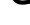
\includegraphics[max width=\textwidth]{2025_04_17_46e04c6acd873ea9558dg-099}
\end{center}

Definim, în acest context, operație drept o instrucțiune de atribuire sau o expresie de incrementare. Care este numărul minim de operații ce se pot executa în secvența de mai sus, în funcție de valoarea citită pentru variabila $n$ ?\\
a) $2 \mathrm{n}-1$\\
b) $n-1$\\
c) 5\\
d) 3\\
e) 2\\
f) 4\\
3. Fie graful orientat $\mathrm{G}=(\mathrm{V}, \mathrm{U})$ unde $\mathrm{V}=\{\mathbf{1}, \mathbf{2}, \mathbf{3}, \mathbf{4}, \mathbf{5}, \mathbf{6}, \mathbf{7}\}$ este mulțimea vârfurilor, iar $\mathrm{U}=\{(2,1),(2,3),(5,2),(5,6),(3,4),(4,5),(4,7)$, $(6,7)$ \} reprezintă mulțimea arcelor. Câte componente tare conexe conține graful?\\
a) 6\\
b) 2\\
c) 3\\
d) 1\\
e) 5\\
f) 4\\
4. Fie arborele cu rădăcină cu nodurile numerotate de la 1 la 15 , reprezentat prin vectorul de tați: $\{3,8,5,5,0,8,3,5,1,7,7,5,4,3,6\}$. Câți descendenți are nodul 3?\\
a) 3\\
b) 4\\
c) 5\\
d) 6\\
e) 2\\
f) 7\\
5. Fie secvența de cod următoare, în care se consideră că variabilele $\mathbf{x}$ și $\mathbf{y}$ rețin numere întregi:

\begin{verbatim}
Limbajul C++
void q (..... , .....)
{ x = 10; y = 20;}
int main() { x = 1; y = 2;
        q(x,y); cout<<<x<<y;
        q(y,x); cout<<x<<<y;
}
Limbajul C
void q (..... , .....)
    {*x = 10; y = 20;}
int main() { x = 1; y = 2;
q(&x,y);printf("%d%d",x,y);
q(&y,x);printf("%d%d",x,y);
}
\end{verbatim}

\begin{verbatim}
Limbajul Pascal
procedure q( ... , ...) ;
    begin
            x := 10; y := 20;
    end;
begin
    x := 1; y := 2;
    q(x,y); write(x,y);
    q(y,x); write(x,y);
end.
\end{verbatim}

Care este varianta corectă a parametrilor formali din antetul subprogramului q pentru care se va afișa secvența 1021010?

\section*{Limbajul C++}
\begin{center}
\begin{tabular}{llllll}
a) & b) & c) & d) & e) & f) \\
int $x$, int $y$ & int $\& x$, int \&y & int $\& x$, int & int $x$, int $\& y$ & int $y$, int $\& x$ & int $y$, int $x$ \\
\end{tabular}
\end{center} y

\section*{Limbajul C}
\begin{center}
\begin{tabular}{|l|l|l|l|l|l|}
\hline
a) & b) & c) & d) & e) & f) \\
\hline
int x , int y & int *x, int * y & int *x, int y & int x , int ${ }^{\text {\% }}$ \% & int y , int ${ }^{\text {* }}$ \% & int y , int x \\
\hline
\end{tabular}
\end{center}

\section*{Limbajul Pascal}
\begin{center}
\begin{tabular}{llllll}
a) & b) & c) & d) & e) & f) \\
x:integer; & var x:integer; & var x: & x:integer; & y:integer; & y:integer; \\
y:integer; & var y: integer; & integer; & var y:integer; & var x:integer; & x:integer; \\
\end{tabular}
\end{center}

\begin{enumerate}
  \setcounter{enumi}{5}
  \item Numărul grafurilor complete orientate cu $\mathbf{2 4}$ de noduri este:\\
a) $\mathbf{2}^{276}$\\
b) $9^{138}$\\
c) $3^{138}$\\
d) $4^{256}$\\
e) $9^{276}$\\
f) $\mathbf{2}^{256}$
  \item Fie secvența de cod următoare în care se consideră că variabilele u și v rețin numere întregi:
\end{enumerate}

\begin{verbatim}
Limbajul C++
int main() { u = 4; v = 4;
cout << u++*++v;
u>v ? cout<<"u" : cout <<"v";}
\end{verbatim}

\begin{verbatim}
Limbajul Pascal
begin
    u:=4; v:=4; inc(v);
    write (u*v);
    if(u>v) then
        write('u')
\end{verbatim}

Limbajul C

\begin{verbatim}
int main() {u = 4; v = 4;
printf("%d",u++*++v);
u>v ? printf("u") :
printf("v");}
\end{verbatim}

\begin{verbatim}
    else
        write('v');
end.
\end{verbatim}

Ce se va afișa în urma rulării secvenței:\\
a) 20 v\\
b) 25 v\\
c) 20 u\\
d) $25 u$\\
e) $16 u$\\
f) 16 v\\
8. Se consideră graful orientat $\mathbf{G}=(\mathbf{V}, \mathbf{U})$ unde $\operatorname{card}(\mathbf{V})=\mathbf{6}$ și $\mathbf{U}=\{(\mathbf{3}, \mathbf{1}),(\mathbf{1}, \mathbf{2}),(\mathbf{2}, \mathbf{3})$, $(4,1),(2,5),(5,3),(3,4)\}$. Indicați numărul minim de muchii ce trebuie eliminate pentru a deveni aciclic?\\
a) 5\\
b) 2\\
c) 3\\
d) 4\\
e) 0\\
f) 1\\
9. Câte grafuri neorientate distincte cu 4 noduri care au adiacente nodurile 1 și 2, respectiv nodurile 3 și $\mathbf{4}$ sunt? Două grafuri se consideră distincte dacă matricile lor de adiacență sunt diferite.\\
a) 18\\
b) 15\\
c) 20\\
d) 12\\
e) 16\\
f) 10\\
10. Fie secvența de cod următoare, unde toate variabilele rețin numere întregi și $\mathrm{n}<\mathrm{m}$ :

\begin{verbatim}
Limbajul C++
int main()
{k=0;
    cin>>n>>m;
for(i=1;i<=n;i++) cin>>v[i];
    for(i=1;i<=m;i++)
    {cin>>x; li=1;ls=n;
        while(li<=ls)
        { m1=(li+ls)/2;
    if(x==v[m1]) {li=ls+1;k++;}
        else
        if(x>v[m1]) li=m1+1;
        else ls=m1-1;}
    }cout<<k; }
Limbajul C
int main( ){
    k=0;scanf("%d%d",&n,&m);
for(i=1;i<=n;i++)
    scanf("%d",&v[i]);
for(i=1;i<=m;i++)
{scanf("%d",&x);li=1;ls=n;
while(li<=ls) {m1=(li+ls)/2;
    if(x==v[m1]) {li=ls+1;k++;}
        else
        if(x>v[m1])li=m1+1;
    k:=0;
    read(n,m);
    for i:=1 to n do
        read(v[i]);
        for i:=1 to m do
            begin
                read(x);
                li := 1; ls := n;
                while(li <= ls) do
                    begin
                        m1 := (li+ls) div 2;
                        if(x = v[m1]) then
                            begin
                                    li:=ls+1; inc(k);
                            end
                                    else
                        if(x>v[m1]) then
                                    li := m1+1
                            else ls := m1-1;
                        end;
                        end;write(k);
end.
\end{verbatim}

Limbajul Pascal\\
begin

\begin{verbatim}
    else ls = m1-1;}
} printf("%d",k);
}
\end{verbatim}

Care este complexitatea acestei secvențe de cod?\\
a) $\mathrm{O}(\mathrm{m} \cdot \log (\mathrm{n}))$\\
b) $O(n \cdot \log m)$\\
c) $O(n \cdot m)$\\
d) $O(n \cdot m \cdot \log n)$\\
e) $O(n \cdot n)$\\
f) $\mathrm{O}(\mathrm{m} \cdot \mathrm{n})$\\
11. Fie secvența de cod următoare:

\begin{verbatim}
Limbajul C++
int f(int a[],int li,int ls)
{ if(li==ls) return a[li];
        else
    return f(a,li,(li+ls)/2) +
f(a,(li+ls)/2+1, ls);}
int main()
{ int n, a[20],i;
cin>>n;
for(i=1;i<=n;i++) cin>>a[i];
    cout<<f(a,1,n);
}
Limbajul C
int f(int a[],int li,int ls)
{
    if(li == ls) return a[li];
        else
    return f(a,li, (li+ls)/2) +
f(a,(li+ls)/2+1, ls);
        }
int main()
{int n,a[20],i;
scanf("%d", &n);
    for(i=1; i<=n; i++)
        scanf("%d", &a[i]);
printf("%d",f(a,1,n));
}
\end{verbatim}

\begin{verbatim}
Limbajul Pascal
type
    vector=array[1..20] of
integer;
var n,i:integer;a:vector;
function f(var a:vector;
li,ls:integer):integer;
begin
if(li=ls) then f:=a[li]
else
f:=f(a,li,(li+ls) div 2)+
f(a,(li+ls) div 2+1, ls ) ;
    end;
begin
        read(n);
        for i:=1 to n do
            read (a[i]) ;
            write(f(a,1,n));
end.
\end{verbatim}

Care este complexitatea acestei secvențe de cod?\\
a) $\mathbf{O}(\mathbf{n} \cdot \log \mathbf{n})$\\
b) $\mathbf{O}(\log n)$\\
c) $\mathbf{O}(\mathbf{n})$\\
d) $\mathbf{O}\left(\mathbf{n}^{2}\right)$\\
e) $\mathbf{O}\left(\mathbf{n}^{2}+1\right)$\\
f) $O\left(n^{2}-1\right)$\\
12. Se consideră un arbore în care fiecare nod intern (nod care nu este pe ultimul nivel) are doi descendenți direcți. Dacă arborele are 38 niveluri (rădăcina se află pe nivelul 0) câte noduri are arborele?\\
a) $\mathbf{2}^{37}$\\
b) $4^{19}-1$\\
c) $\mathbf{2}^{38}+1$\\
d) $2^{37}+1$\\
e) $2^{33}+1$\\
f) $2^{39}$\\
13. Ce se va afișa pentru secvența de cod:

\begin{verbatim}
Limbajul C++
int x,y;
void f(int &y, int x)
    {x++; y=y+x;}
int main() {
x = 4; y = 2;cout<<x<<<y<<" ";
f(x,y); cout<<x<<<y<<" ";
f(x,x) ; cout<<x<<<y<<" ";
f(y,x); cout<<x<<<y<<" ";}
Limbajul C
int x,y;
void f(int *y,int x)
{x++;*y=*y+x;}
int main() {
x = 4; y = 2;printf("%d%d ",x,y);
f(&x,y); printf("%d%d ", x,y);
f(&x,x); printf("%d%d ", x,y);
f(&y,x); printf("%d%d ", x,y); }
\end{verbatim}

\begin{verbatim}
Limbajul Pascal
var x,y:integer;
procedure f(var y:integer;
x:integer) ;
    begin
        inc(x);
        y:=y+x;
    end;
begin
    x:=4;y:=2;write(x,y,' ');
        f(x,y) ; write(x,y,' ');
        f(x,x) ; write(x,y,' ');
        f(y,x); write(x,y,' ');
        end.
\end{verbatim}

a) $42 \quad 72 \quad 152 \quad 1518$\\
b) $42 \quad 215 \quad 42518$\\
c) $42 \quad 27 \quad 415 \quad 158$\\
d) $42 \quad 62 \quad 41 \quad 58$\\
e) $42 \quad 62 \quad 45 \quad 58$\\
f) $42 \quad 72 \quad 415 \quad 58$\\
14. Folosind algoritmul de sortare prin inserție, pentru ordonarea crescătoare a tabloului unidimensional $v=[6,5,4,3,2,1]$ se efectuează 45 de pași (de exemplu pentru deplasarea elementului cu valoarea 6 pe poziția 2 se execută 5 pași):\\
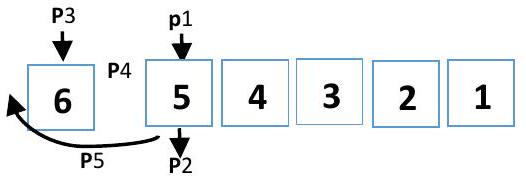
\includegraphics[max width=\textwidth, center]{2025_04_17_46e04c6acd873ea9558dg-103}

\begin{verbatim}
P1: i\leftarrow2
P2: }x\leftarrowv[i
P3: j\leftarrowi-1;
P4: v[j+1]}\leftarrowv[j]
P5: v[j]}\leftarrowx
\end{verbatim}

Precizați câți pași se execută folosind același algoritm pentru ordonarea crescătoare a tabloului $\mathrm{v}=[1000,999, \ldots, 3,2,1]$\\
a) $\mathbf{1 0 0 1 9 9 9}$\\
b) 1001997\\
c) $\mathbf{1 0 0 1 9 9 8}$\\
d) $\mathbf{1 0 0 2 0 0 0}$\\
e) 1001897\\
f) 1001887\\
15. Fie subprogramul de mai jos:

\begin{verbatim}
Limbajul C++
void f(int n,int k) {int i;
for(i = 1; i <= n; i++)
    {if(i%k == O) cout<<i<<" ";
        f(n-1,k);}}
\end{verbatim}

\section*{Limbajul C}
\begin{verbatim}
Limbajul Pascal
procedure f (n,k:integer);
var i : integer;
    begin
        for i := 1 to n do
            begin
            if(i mod k = O) then
                write(i,' ');
\end{verbatim}

\begin{verbatim}
void f(int n,int k) {int i;
for(i = 1; i <= n; i++)
{if(i%k==0) printf("%d
",i);
    f(n-1,k);} }
        f(n-1,k);
    end;
end;
\end{verbatim}

De câte ori se execută instrucțiunea de decizie în cadrul subprogramului, dacă apelul este $\mathbf{f}(3,1)$ ?\\
a) $\mathbf{1 5} \mathrm{ori}$\\
b) $\mathbf{1 4}$ ori\\
c) $\mathbf{1 6} \mathbf{~ o r i}$\\
d) 8 ori\\
e) 9 ori\\
f) $\mathbf{1 0} \mathbf{~ o r i}$

\begin{enumerate}
  \item Fie subprogramul:
\end{enumerate}

\begin{verbatim}
Limbajul C/C++
    int f (int n, int s){
    if (n < s) return 0;
    else
    if(n%s == 0)
            return 1+ f(n/s,s+1);
        else
            return f(n/s,s);
    }
\end{verbatim}

\begin{verbatim}
Limbajul Pascal
function f(n,s:integer):
integer;
begin
    if (n < s) then f:=0
    else if (n mod s =0) then
        f:= 1 + f(n div s,s+1)
        else f:= f(n div s,s);
    end;
\end{verbatim}

Subprogramul se execută pentru următoarele seturi de valori $n=720, s=2$; $\mathrm{n}=120, \mathrm{~s}=3 ; \mathrm{n}=120, \mathrm{~s}=1$; $\mathrm{n}=720, \mathrm{~s}=1$. Pentru câte dintre apeluri subprogramul f va returna valoarea 5 ?\\
a) un apel\\
b) 2 apeluri\\
c) 3 apeluri\\
d) niciun apel\\
e) 4 apeluri\\
f) 5 apeluri\\
2. Fie subprogramul de mai jos unde $\mathbf{n}$ și $\mathbf{c}$ sunt variabile întregi:

\begin{verbatim}
Limbajul C++
int f(int &n, int c) {
    int a = n%10;
    if(n == 0) return 0;
    else
    if(a == c)
        {n=n/10;
return 1+f(n,c);}
        else
    {n=n/10%10;return f(n,c);
}}
Limbajul C
int f (int *n, int c) {
    int a = *n %10;
    if(*n == 0) return 0;
    else
    if(a==c)
        {*n=*n/10;
return 1+f(n,c);}
            else
    {*n=(*n)/10%10;
            return f(n,c);}
    }
\end{verbatim}

Care sunt variabilele ale căror valori sunt reținute în stiva subprogramului?\\
a) $\mathrm{n}, \mathrm{c}, \mathrm{a}$\\
b) c , a\\
c) $n, c$\\
d) a\\
e) c\\
f) $n, a$

Limbajul Pascal function $f(v a r \quad n$ :integer; c:integer) : integer; var a : integer; begin a $:=\mathrm{n} \bmod 10$; if $(\mathrm{n}=0)$ then $\mathrm{f}:=0$ else if ( $a=c$ ) then begin $\mathrm{n}:=\mathrm{n} \operatorname{div} 10 ;$ $\mathrm{f}:=1+\mathrm{f}(\mathrm{n}, \mathrm{c})$; end else begin $\mathrm{n}:=\mathrm{n}$ div $10 \bmod 10 ;$ $\mathrm{f}:=\mathrm{f}(\mathrm{n}, \mathrm{c})$; end; end;\\
3. Fie $\mathbf{G}$ un graf neorientat $\mathrm{cu} \mathrm{n}>0$ vârfuri și $\mathrm{m}>0$ muchii, reprezentat prin liste de adiacență. Complexitatea unui algoritm care afișează matricea de adiacență asociată grafului este:\\
a) $\mathbf{O}(m \cdot \log n)$\\
b) $\mathbf{O}(\mathbf{m} \cdot \mathbf{n})$\\
c) $\mathbf{O}\left(\mathbf{n}^{2}\right)$\\
d) $\mathbf{O}\left(\mathrm{m}^{2}\right)$\\
e) $\mathbf{O}\left(\mathrm{m}^{2}+\mathbf{1}\right)$\\
f) $\mathbf{O}\left(\mathrm{m}^{2}-1\right)$\\
4. Variabilele $\mathbf{x}$ și $\mathbf{y}$ rețin numere întregi.Care dintre expresiile de mai jos are valoarea 1 (Limbajul C/C++), True (Limbajul Pascal) știind că $\mathbf{x}>-1$ și $\mathbf{y}<3$ ?\\
Limbajul C/C++\\
a) $\mathbf{x *} \mathbf{y}+\mathbf{y}-3 * \mathbf{x}-3>0$\\
b)! ( $\left.x^{*} y+y-3 * x-3>=0\right)$\\
c) $(x-1) *(y-3)<0$\\
d) $(x+1) *(y-3)>0$\\
e) $(x-1) *(y+3)>0$\\
f) $(x+1) *(y+3)>0$

Limbajul Pascal\\
a) $\mathbf{x *} \mathbf{y}+\mathbf{y}-3 * \mathbf{x}-3>0$\\
b)NOT ( $x$ * $y+y-3 * x-3>=0$ )\\
c) $(x-1) *(y-3)<0$\\
d) $(x+1) *(y-3)>0$\\
e) $(x-1) *(y+3)>0$\\
f) $(x+1) *(y+3)>0$\\
5. Se consideră numărul natural $\mathrm{n}=231045$. Dacă se determină toate submulțimile formate din cifrele lui $\mathbf{n}$ care au suma valorilor componentelor egală cu 10 , câte submulțimi conțin cifra 0 ?\\
a) 3\\
b) 5\\
c) 2\\
d) 1\\
e) 4\\
f) 6\\
6. Se consideră șirul $\{\mathbf{a}, \mathbf{b}, \mathbf{c}, \mathbf{u}, \mathbf{i}, \mathbf{e}\}$. Se generează folosind metoda backtracking, în ordine lexicografică, toate cuvintele de trei litere distincte, care conțin două vocale. Dacă primele trei soluții sunt abe , abi , abu care este a 9 -a soluție?\\
a) aic\\
b) aib\\
c) $a e c$\\
d) $a u b$\\
e) ace\\
f) aei\\
7. În câte moduri se poate scrie numărul 12 ca sumă de numere prime?\\
a) 5\\
b) 3\\
c) 7\\
d) 6\\
e) 5\\
f) 4\\
8. Se consideră mulțimea de cuvinte \{info, mate, fizica, chimie, biologie\}. Se generează folosind metoda backtracking, lexicografic, în ordinea inversă citirii cuvântului, submultimi de câte trei cuvinte distincte. Dacă primele trei soluții sunt: \{fizica, biologie, chimie\};\{fizica, biologie, mate\};\{fizica, biologie, info\}; înaintea soluției \{chimie, mate, info\} este soluția:\\
a) $\{$ biologie, mate,info $\}$\\
b) \{biologie, chimie,mate\}\\
c) $\{$ chimie, biologie, info $\}$\\
d) \{chimie,mate,biologie\}\\
e) \{fizica, mate,biologie\}\\
f) $\{$ chimie,fizica, biologie $\}$\\
9. Se consideră un arbore cu rădăcină în care fiecare nod intern (nod care nu este pe ultimul nivel) are doi descendenți direcți. Dacă arborele are $\mathbf{k}$ niveluri (rădăcina se află pe nivelul 0) câte noduri sunt pe nivelul $\mathbf{k}$ ?\\
a) $2^{\mathrm{k}+1}$\\
b) $2^{\mathrm{k}-1}+1$\\
c) $\mathbf{2}^{k}$\\
d) $2^{\mathrm{k}-1}$\\
e) $\mathbf{2}^{\mathrm{k}-2}+\mathbf{1}$\\
f) $2^{k+1}+1$\\
10. Se consideră șirul primelor $n \times m$ numere naturale unde $n \geq 1$ și $m \geq 1$. Dacă se afișează câte $\mathbf{m}$ numere pe o linie, numărul 123 se află pe linia 4 și coloana 3 , atunci pe ce linie și coloană se află numărul 167?\\
a) linia 5 ,\\
b) linia 4,\\
c) linia 6,\\
d) linia 6,\\
e) linia 5,\\
f) linia 5, coloana 7 coloana 7 coloana 4 coloana 2 coloana 2 coloana 3\\
11. Fie secvența de cod următoare în care se consideră că variabilele $\mathbf{a}, \mathbf{i}, \mathrm{n}$ rețin numere întregi.

\begin{verbatim}
Limbajul C++
int main() {
    cin>>n; a = 1; i = 2;
while (i<n && a>0) {
    if(n%i == 0) a = 0;
            else i++; cout<<i;
}}
Limbajul C
int main(){ scanf("%d",&n);
a = 1; i = 2;
    while (i<n &&a>0){
        if(n%i == 0) a = 0;
            else i++;
printf("%d",i);
} }
\end{verbatim}

\begin{verbatim}
Limbajul Pascal
read(n); a := 1; i := 2;
while (i<n) and (a>0) do
        begin
        if(n mod i = 0) then
                a:=0
            else
                inc(i);
            write(i);
    end;
\end{verbatim}

Definim, în acest context, operație drept o instrucțiune de atribuire sau o expresie de incrementare. Care este numărul maxim de operații ce se pot executa în secvența de mai sus, în funcție de valoarea citită pentru variabila $n$ ?\\
a) $2 n+2$\\
b) 2 n\\
c) $\mathrm{n}-1$\\
d) $2 n+3$\\
e) $n$\\
f) $n+1$\\
12. Fie secvența de program unde variabila i reține un număr întreg:

\begin{verbatim}
Limbajul C++
    i = 4;
while (i <= 25)
    {cout<<i/10+i%10<<" ";
i+=2;
}
\end{verbatim}

Limbajul C

\begin{verbatim}
i = 4;
while (i <= 25)
{printf("%d ",i/10+i%10);
i+=2;
}
\end{verbatim}

Ultimele trei numere afișate sunt:\\
a) 247\\
b) 249\\
c) 624\\
e) 246\\
f) 921\\
13. Fie secvența de cod de mai jos:

\begin{verbatim}
Limbajul C/C++
float s,p;
float s1(int n) {
if(n==0) return 2;else
if(n==1) return s;else
return s*s1(n-1)-
    p*s1(n-2);
}
\end{verbatim}

\begin{verbatim}
Limbajul Pascal
var s,p : float;
function s1(n : integer) :
real;
begin
if (n = 0) then s1:=2
else
if (n = 1) then s1:=s
else s1:=s*s1(n-1)-p*s1(n-2);
end;
\end{verbatim}

Dacă la apelul subprogramului s1 se returnează valoarea 82, ce valori inițiale au variabilele $\mathbf{n}, \mathbf{s}$ și $\mathbf{p}$ în această ordine?\\
a) 434\\
b) 443\\
c) 423\\
d) 332\\
e) 312\\
f) 342\\
14. Fie secvența de cod unde toate variabilele sunt întregi:

\begin{verbatim}
Limbajul C++
s=0; cin>>n>>k;
for(i=1;i<=n;i++)
    for(j=1;j<=n;j++)
{ if (i > j) t = i - j;
        else t = j - i;
        if(i==j || t<=k || j==n-i+1 || (i+j>=n-k+1 && i+j<=n+k+1))
                a[i][j] = 1;
        else a[i][j] = 2;
    if(a[i][j] == 2) s++;}
\end{verbatim}

Limbajul C

\begin{verbatim}
s=0; scanf("%d%d",&n,&k);
for(i=1;i<=n;i++)
    for (j=1;j<=n;j++)
    {if (i > j) t = i - j;
        else t = j - i;
        if(i==j || t<=k || j==n-i+1 || (i+j>=n-k+1 && i+j<=n+k+1))
                    a[i][j] = 1;
            else a[i][j] = 2;
                if(a[i][j] == 2) s++;}
\end{verbatim}

Limbajul Pascal

\begin{verbatim}
s:=0; read(n,k);
for i:=1 to n do
    for j:=1 to n do
        begin
            if(i>j) then t:=i-j
            else t:=j-i;
            if((i=j) or (t<=k) or (j=n-i+1) or ((i+j>=n-k+1) and (i+j<=
n+k+1))) then a[i,j]:=1
\end{verbatim}

\begin{verbatim}
else a[i,j]:=2;
if(a[i,j] = 2) then inc(s);
    end;
\end{verbatim}

Pentru ce valori ale lui $\mathbf{n}$ și $\mathbf{k}$ variabila $\mathbf{s}$ va avea valoarea $\mathbf{8}$ ?\\
a) $\mathbf{n}=\mathbf{6 ; ~} \mathrm{k}=\mathbf{2}$\\
b) $\mathrm{n}=6$; $k=1$\\
c) $\mathbf{n}=5 ; \mathbf{k}=\mathbf{2}$\\
d) $\mathbf{n}=7 ; \mathbf{k}=1$\\
e) $\mathbf{n}=\mathbf{4} ; \mathbf{k}=\mathbf{2}$\\
f) $\mathbf{n}=6 ; k=3$\\
15. Se consideră un tablou bidimensional în care $\mathbf{a}$ [i] [j]=j+3(i-1), $(1 \leq i, j \leq 3)$ Fie secvența de cod de mai jos:

\begin{verbatim}
Limbajul C++
k = 0;
for(i=1; i<=3; i++)
{for(j =1; j<=3-k; j++)
        cout<<a[\alpha][\beta]<<" ";
            k++; }
\end{verbatim}

Limbajul C\\
k=0;\\
for (i=1; i<=3; i++)\\
\{for (j =1; $\mathrm{j}<=3-\mathrm{k} ; \mathrm{j}++$ )\\
printf("\%d ",a[ $\alpha$ ] [ $\beta$ ]);\\
k++; \}

\begin{verbatim}
Limbajul Pascal
$$
\mathrm{k}:=0 \text {; }
$$
$$
\text { for i:=1 to } 3 \text { do }
$$
    begin
        for j:=1 to 3-k do
            write(a[\alpha,\beta],' ');
        inc(k); end;
\end{verbatim}

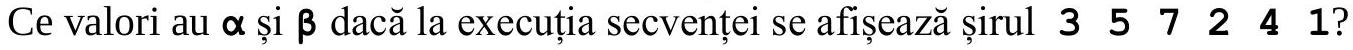
\includegraphics[max width=\textwidth, center]{2025_04_17_46e04c6acd873ea9558dg-109}\\
а) $\boldsymbol{\alpha}=\mathbf{3}-\mathbf{j}-\mathbf{k}$;\\
b) $\boldsymbol{\alpha}=\mathrm{j}$;\\
c) $\alpha=\mathrm{j}$;\\
d) $\boldsymbol{\alpha}=4-j-k$;\\
e) $\boldsymbol{\alpha}=\mathbf{4}+\mathbf{j}-\mathbf{k}$;\\
f) $\alpha=4+j+k ;$ $\boldsymbol{\beta}=\mathbf{j}$ $\beta=3-j-k$ $\beta=4-j-k$ $\boldsymbol{\beta}=\mathbf{j}$ $\boldsymbol{\beta}=\mathbf{j}-\mathbf{1}$ $\boldsymbol{\beta}=\mathbf{j}+1$

\section*{Varianta 21}
\begin{enumerate}
  \item Precizați care dintre următoarele expresii are valoarea true în Pascal sau 1 în C/C++ dacă și numai dacă numărul întreg $\mathbf{x}$ are exact trei cifre?
\end{enumerate}

Limbajul C++\\
a) $(x \% 1000==0)$ || $(x \% 100!=0)$\\
b) $(x / 10==0) \& \&(x / 100==0)$\\
c) $(x \% 10==0) \& \&(x / 10==0)$\\
d) $(x / 1000==0) \& \&(x / 100!=0)$\\
e) $(x / 1000==0)$ || $(x / 100==0)$\\
f) ! ( $(x / 1000==0) \& \&(x / 100!=0))$

Limbajul C\\
a) $(x \% 1000==0)|\mid(x \% 100!=0)$\\
b) $(x / 10==0) \& \&(x / 100==0)$\\
c) $(x \% 10==0) \& \&(x / 10==0)$\\
d) $(x / 1000==0) \& \&(x / 100!=0)$\\
e) $(x / 1000==0)$ || $(x / 100==0)$\\
f)! ( $(x / 1000==0) \& \&(x / 100!=0))$

\section*{Limbajul Pascal}
a) ( $x \bmod 1000=0$ ) or ( $x$ mod 100<>0)\\
b) ( $x \operatorname{div} 10=0$ ) and ( $x$ div 100=0)\\
c) ( $x \bmod 10=0$ ) and ( $x$ div 10=0)\\
d) ( $x$ div $1000=0$ ) and ( $x$ div 100<>0)\\
e) ( $x \operatorname{div} 1000=0$ ) or ( $x$ div 100=0)\\
f) $\operatorname{not}((x \operatorname{div} 1000=0)$ and (x div 100<>0))\\
2. Roboțelul Bob se mișcă într-un plan cartezian. Pentru a reține poziția robotului definim următoarea structură:

\begin{verbatim}
Limbajul C
typedef struct
{
    float x,y;
} robot;
robot bob;
\end{verbatim}

\begin{verbatim}
Limbajul C++
struct robot
{
    float x,y;
};
robot bob;
\end{verbatim}

\begin{verbatim}
Limbajul Pascal
type robot=record
    x,y:real;
    end;
var bob:robot;
\end{verbatim}

Precizați care dintre expresiile de mai jos este adevărată dacă și numai dacă roboțelul se află în interiorul sau pe laturile pătratului de coordonate $(-2,-2),(-2,2)$, $(2,2),(2,-2)$ ?\\
Limbajul C++\\
a) (robot. $x>=-2) \& \&($ robot $. x<=2) \& \&($ robot. $y>=-2) \& \&($ robot. $y<=2)$\\
b) (robot. $x<=-2$ ) || (robot. $x>=2$ ) || (robot. $y<=-2$ ) || (robot.y>=2)\\
c) (bob. $x<=-2$ ) || (bob $\cdot x>=2$ ) || (bob. $y>=-2$ ) || (bob. $y<=2$ )\\
d) (bob $\cdot x>=-2) \& \&(b o b . x<=2) \& \&(b o b . y>=-2) \& \&(b o b . y<=2)$\\
e) (bob $\cdot x>=-2) \& \&(b o b . x<=2)|\mid(b o b . x>=-2) \& \&(b o b . x<=2)$\\
f) (robot. $x>=-2$ ) $\& \&($ robot $. x<=2)|\mid($ robot $. x>=-2) \& \&($ robot $. x<=2)$

\section*{Limbajul C}
a) (robot. $x>=-2$ ) $\& \&($ robot $. x<=2) \& \&($ robot. $y>=-2) \& \&($ robot. $y<=2)$\\
b) (robot. $x<=-2$ ) || (robot. $x>=2$ ) || (robot. $y<=-2$ ) || (robot. $y>=2$ )\\
c) (bob $\cdot x<=-2)||(b o b . x>=2)||(b o b . y>=-2)|\mid(b o b . y<=2)$\\
d) (bob $\cdot x>=-2) \& \&(b o b . x<=2) \& \&(b o b . y>=-2) \& \&(b o b . y<=2)$\\
e) (bob $\cdot x>=-2) \& \&(b o b . x<=2)|\mid(b o b . x>=-2) \& \&(b o b . x<=2)$\\
f) (robot. $x>=-2$ ) \&\& (robot. $x<=2$ ) || (robot. $x>=-2$ ) $\& \&($ robot. $x<=2)$

Limbajul Pascal\\
a) (robot. $x>=-2$ ) and (robot. $x<=2$ ) and (robot.y>=-2) and (robot. $\mathrm{y}<=2$ )\\
b) (robot. $x<=-2$ ) or (robot. $x>=2$ ) or (robot. $y<=-2$ ) or (robot. $\mathrm{y}>=2$ )\\
c) (bob. $x<=-2$ ) or (bob. $x>=2$ ) or (bob.y>=-2) or (bob.y<=2)\\
d) (bob. $x>=-2$ ) and (bob. $x<=2$ ) and (bob. $y>=-2$ ) and (bob. $y<=2$ )\\
e) (bob. $x>=-2$ ) and (bob. $x<=2$ ) or (bob. $x>=-2$ ) and (bob. $x<=2$ )\\
f) (robot. $x>=-2$ ) and (robot. $x<=2$ ) or (robot. $x>=-2$ ) and (robot. $x<=2$ )\\
3. Precizați ce se va afișa în urma execuției următorului program?

\begin{verbatim}
Limbajul C++
#include <iostream>
using namespace std;
int main()
{ int i,s=0;
    for(i=1;i<=5;i++);
        s=s+i;
    cout<<s; return 0;}
\end{verbatim}

\begin{verbatim}
Limbajul Pascal
var i,s:integer;
begin
s:=0;
for i:=1 to 5 do;
    i:=i+1;
s:=s+i; write(s);
end.
\end{verbatim}

\begin{verbatim}
Limbajul C
#include <stdio.h>
int main()
{ int i,s=0;
    for(i=1;i<=5;i++);
        s=s+i;
    printf("%d",s); return 0; }
\end{verbatim}

a) Programul nu va afișa nimic, va\\
b) 15\\
c) 6\\
d) 5\\
e) 0\\
f) 10 genera eroare de compilare.\\
4. Precizați ce se va afișa pe ecran în urma execuției următorului program?

\begin{verbatim}
Limbajul C++
#include <iostream>
using namespace std;
int main()
{
    char sir[]="ANA";
        int i=0;
        while(sir[i])
            sir[i++]++;
        cout<<sir;
        return 0;
}
\end{verbatim}

\begin{verbatim}
Limbajul Pascal
var sir:string;
        i:integer;
begin
    sir:='ANA';
    for i:=1 to length(sir) do
            sir[i]:=succ(sir[i]);
    write(sir);
end.
\end{verbatim}

\begin{verbatim}
Limbajul C
#include <stdio.h>
int main()
{ char sir[]="ANA";
    int i=0;
    while(sir[i])
        sir[i++]++;
    printf("%s",sir);
    return 0;
\end{verbatim}

\}\\
a) ANA\\
b) $\mathbf{A}$\\
c) AN\\
d) BOB\\
e) $B A B$\\
f) COC\\
5. Precizați ce se va afișa pe ecran în urma execuției următorului program?

\begin{verbatim}
Limbajul C++
#include <iostream>
using namespace std;
struct coordonate{
    int abscisa,ordonata;
};
int main()
{ coordonate abscisa;
    abscisa.abscisa=100;
    abscisa.ordonata=200;
cout<<abscisa.abscisa<<" ";
    cout<<abscisa.ordonata;
    return 0;}
\end{verbatim}

\begin{verbatim}
Limbajul Pascal
type coordonate=record
abscisa,ordonata:integer;
end;
var abscisa:coordonate;
begin
abscisa.abscisa:=100;
abscisa.ordonata:=200;
write(abscisa.abscisa,' ');
write(abscisa.ordonata);
end.
\end{verbatim}

\begin{verbatim}
Limbajul C
\#include <stdio.h>
typedef struct \{ int abscisa,ordonata;
\} coordonate;
int main()
\{
coordonate abscisa;
    abscisa.abscisa=100;
    abscisa.ordonata=200;
    printf("%d ",abscisa.abscisa);
    printf("%d", abscisa.ordonata);
    return 0;
}
\end{verbatim}

a) Programul nu va afișa\\
b) 00\\
c) $\mathbf{1 0 0} \mathbf{2 0 0}$\\
d) 200100\\
e) 100100\\
f) 200200

\begin{verbatim}

\end{verbatim}

\begin{enumerate}
  \setcounter{enumi}{5}
  \item Care va fi valoarea returnată de funcția f prezentată mai jos?
\end{enumerate}

\begin{verbatim}
Limbajul C/C++
char f()
{ int i,j,mat[5][5];
    char v='a';
    for(i=0;i<5;i++)
        for(j=0;j<5;j++)
            { mat[i][j]=v;
                    v++; }
            return mat[2][3]; }
\end{verbatim}

\begin{verbatim}
Limbajul Pascal
type matrice=array[0..4,0..4] of
                    char;
function f:char;
    var i,j:integer;
        mat:matrice;
        v:char;
begin
    v:='a';
    for i:=0 to 4 do
        for j:=0 to 4 do
            begin
            mat[i,j]:=v;v:=succ(v);
            end;
    f:=mat[2,3];
end;
\end{verbatim}

a) e\\
b) i\\
c) $n$\\
d) $m$\\
e) 0\\
f) $p$\\
7. Se consideră graful neorientat $G$ reprezentat prin următoarea matrice de adiacență:

$$
A=\left(\begin{array}{lllllll}
0 & 1 & 1 & 0 & 0 & 0 & 0 \\
1 & 0 & 1 & 0 & 0 & 0 & 0 \\
1 & 1 & 0 & 0 & 0 & 0 & 0 \\
0 & 0 & 0 & 0 & 1 & 0 & 0 \\
0 & 0 & 0 & 1 & 0 & 0 & 0 \\
0 & 0 & 0 & 0 & 0 & 0 & 0 \\
0 & 0 & 0 & 0 & 0 & 0 & 0
\end{array}\right)
$$

Precizați numărul componentelor conexe ale grafului $\mathbf{G}$.\\
a) 1\\
b) 2\\
c) 3\\
d) 4\\
e) 5\\
f) 6\\
8. Corectați secvența de program de mai jos astfel încât să realizeze corect căutarea unui număr întreg $\mathbf{x}$ într-un vector $\mathbf{v}$ cu $n$ elemente numere intregi ordonate crescător.

\begin{verbatim}
Limbajul C/C++
p=0;
u=n-1;
q=0;
while(p<=u && q==0)
{
    m=(p+u)/2;
    if(x==v[m]) q=1;
    else if(x<v[m]) u=m-1;
            else p=m-1;
    }
if(q==1)
        printf("Elementul a fost
gasit");
    else
\end{verbatim}

\begin{verbatim}
Limbajul Pascal
p:=0;
u:=n-1;
q:=0;
while (p<=u) and (q=0) do
begin
    m:=(p+u) div 2;
    if(x=v[m]) then q:=1
    else if x<v[m] then u:=m-1
            else p:=m-1;
    end;
    if q=1 then
write('Elementul a fost
gasit')
    else
\end{verbatim}

\begin{verbatim}
    printf("Elementul nu a
fost gasit");
Limbajul C/C++
a) Instrucțiunea
    while(p<=u && q==0)
    trebuie înlocuită cu
    while(p>=u && q==0)
b) Instrucțiunea m=(p+u)/2;
    trebuie înlocuită cu m= (p+u) %2;
c) Instrucțiunea p=m-1; trebuie
    înlocuită cu p=m+1;
d) Instrucțiunea u=m-1; trebuie
    înlocuită cu u=m+1;
e) Instrucțiunea if (x<v [m]) trebuie
    înlocuită cu if (x>v [m])
f) Instrucțiunea q=1 ; trebuie îlocuită
    cu q=0 ;
\end{verbatim}

\begin{verbatim}
9. Precizați ce se va afișa pe ecran în urma execuției programului următor?
Limbajul C++
#include <iostream>
using namespace std;
int main()
{ const int m=4,n=5;
        int i,j,aux;
        char a[m][n]=
            {{'a','b','c','d','e'},
            {'f','g','h','i','j'},
            {'k','l','m','n','o'},
            {'p','q','r','s','t'}};
for(i=0;i<2;i++)
    { aux=a[2][n-1];
        for(j=n-1;j>0;j--)
                    a[2][j]=a[2][j-1];
        a[2][0]=aux; }
for(i=0;i<2;i++)
        { aux=a[m-1][2];
                for(j=m-1;j>0;j--)
                        a[j][2]=a[j-1][2];
                a[0][2]=aux; }
for(i=0;i<m;i++) {
        for(j=0;j<n;j++)
                cout<<a[i][j]<<" ";
\end{verbatim}

\begin{verbatim}
write('Elementul nu a
fost gasit');
\end{verbatim}

\section*{Limbajul Pascal}
a) Instrucțiunea while ( $p<=u$ ) and ( $q=0$ ) do trebuie înlocuită cu

\begin{verbatim}
while (p>=u) and (q=O) do
\end{verbatim}

b) Instrucțiunea $\mathrm{m}:=(\mathrm{p}+\mathrm{u}) \operatorname{div} 2$; trebuie înlocuită cu m:=(p+u) mod 2;\\
c) Instrucțiunea $p:=m-1$; trebuie înlocuită cu p:=m+1;\\
d) Instrucțiunea $u:=m-1$; trebuie înlocuită cu u:=m+1;\\
e) Instrucțiunea if $\mathbf{x}<\mathbf{v}$ [m] trebuie înlocuită cu if $x>v[m]$\\
f) Instrucțiunea $\mathrm{q}:=1$; trebuie înlocuită cu q: =0;

\begin{verbatim}
Limbajul Pascal
const m=4; n=5;
var i,j:integer;
        aux:char;
    a:array[0..m-1,0..n-1]
        of char=
(('a','b','c','d','e'),
('f','g','h','i','j'),
('k','l','m','n','o'),
('p','q','r','s','t'));
begin
for i:=0 to 1 do
    begin
            aux:=a[2,n-1];
        for j:=n-1 downto 1 do
                    a[2,j]:=a[2,j-1];
            a[2,0]:=aux; end;
for i:=0 to 1 do
    begin
            aux:=a[m-1,2];
        for j:=m-1 downto 1 do
                    a[j,2]:=a[j-1,2];
            a[0,2]:=aux; end;
for i:=0 to m-1 do
\end{verbatim}

\begin{verbatim}
    cout<<endl; }
return 0; }
\end{verbatim}

\begin{verbatim}
begin
    for j:=0 to n-1 do
        write(a[i,j],' ');
    writeln; end;
end.
\end{verbatim}

\begin{verbatim}
Limbajul C
#include <stdio.h>
int main()
{ const int m=4,n=5;
    int i,j,aux;
    char a[4][5]={{'a','b','c','d','e'},
                {'f','g','h','i','j'},
                {'k','l','m','n','o'},
                {'p','q','r','s','t'}};
for(i=0;i<2;i++)
    { aux=a[2][n-1];
        for(j=n-1;j>0;j--)
            a[2][j]=a[2][j-1];
        a[2][0]=aux;
        }
for(i=0;i<2;i++)
    {
        aux=a[m-1][2];
        for(j=m-1;j>0;j--)
            a[j][2]=a[j-1][2];
        a[0][2]=aux;
        }
for(i=0;i<m;i++) {
        for(j=0;j<n;j++)
    printf("%c %c",a[i][j],' ');
            printf("\n");
        }
return 0;
}
\end{verbatim}

\begin{center}
\begin{tabular}{|l|l|l|l|l|l|}
\hline
a) & b) & c) & d) & e) & f) \\
\hline
abcde & abmde & deabc & abkde & edcba & abcde \\
\hline
fghij & fgrij & ijfgh & fgrij & fghij & fghij \\
\hline
noklm & klcno & lmnok & noclm & klmo & klmo \\
\hline
pqrst & pqhst & stpqr & pqhst & pqrst & tsrqp \\
\hline
\end{tabular}
\end{center}

\begin{enumerate}
  \setcounter{enumi}{9}
  \item Precizați ce se va afișa pe ecran în urma execuției următorului program?
\end{enumerate}

\begin{verbatim}
Limbajul C++
#include <iostream>
using namespace std;
int a=5, b=10, c=15;
void f(int a,int &b,int &c)
{ a=a+5; b=b+10; c=c+15;
\end{verbatim}

\begin{verbatim}
Limbajul Pascal var a,b,c:integer;
procedure f(a:integer;var
b:integer; var
c:integer);
begin
\end{verbatim}

\begin{verbatim}
}
int main()
{f(a,b,c);f(a,a,b);
    cout<<"a="<<a;
    cout<<"b="<<b;
    cout<<"c="<<c;
    return 0;
}
\end{verbatim}

\begin{verbatim}
    a:=a+5;b:=b+10;c:=c+15;
end;
begin
    a:=5; b:=10; c:=15;
    f(a,b,c);f(a,a,b) ;
    write('a=',a);
    write('b=',b);
    write('c=',c);
end.
\end{verbatim}

Limbajul C\\
\#include <stdio.h>\\
int $a=5, b=10, c=15$;\\
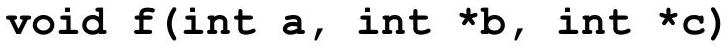
\includegraphics[max width=\textwidth, center]{2025_04_17_46e04c6acd873ea9558dg-116}\\
$\{a=a+5 ; * b=* b+10 ; * c=* c+15 ;\}$\\
int main()\\
$\{\mathrm{f}(\mathrm{a}, \& \mathrm{~b}, \& \mathrm{c}) ; \mathrm{f}(\mathrm{a}, \& \mathrm{a}, \& \mathrm{~b})$;\\
printf("a=\%d", a ) ; printf("b=\%d",b) ; printf("c=\%d",c);\\
return 0; \}\\
a) $\mathbf{a}=5$\\
b) $\mathbf{a}=15$\\
c) $\mathbf{a}=10$\\
d) $\mathbf{a}=5$\\
e) $\mathbf{a}=15$\\
f) $\mathbf{a}=10$\\
$b=5$\\
$b=35$\\
$b=20$\\
$b=10$\\
b=5\\
$b=5$\\
$c=20$\\
$\mathrm{c}=30$\\
$\mathrm{c}=30$\\
$\mathrm{c}=15$\\
$c=30$\\
$\mathrm{c}=30$\\
11. Un echipaj va pleca spre Marte în misiunea POLI. El este alcătuit din căpitan 1 - Andrei, căpitan 2 - Marian și cercetătorii Alina, Dana și Marius. Săptămânal membrii echipajului trebuie să transmită un raport respectând o anumită ordine: întotdeauna raportul căpitanului 1 trebuie să fie înaintea raportului căpitanului 2. Știind că primele trei soluții posibile de raportare sunt:\\
Andrei Marian Alina Dana Marius\\
Andrei Marian Alina Marius Dana\\
Andrei Marian Dana Alina Marius\\
afișați a zecea soluție.\\
a) Marius\\
Dana\\
Alina\\
Andrei\\
Marian\\
b) Dana\\
Marius\\
Alina\\
Andrei\\
Marian\\
c) Marius\\
Andrei\\
Marian\\
Alina\\
Dana\\
d) Andrei\\
Alina\\
Dana\\
Marius\\
Marian\\
e) Andrei Alina\\
Dana\\
Marian\\
Marius\\
f) Andrei Alina Marius\\
Marian\\
Dana\\[0pt]
12. Înlocuiți valoarea lui v[3] cu una dintre următoarele valori astfel încât funcția să returneze 0 în C/C++ sau false în Pascal pentru apelul $f(5)$.

\begin{verbatim}
Limbajul C++
int $v[]=\{15,12,7,20,-1,-5\}$;
int $f(i n t n)$
\{if(n==0) return 0;
else
return
$v[n-1]<v[n]| | f(n-1) ;\}$
\end{verbatim}

\begin{verbatim}
Limbajul Pascal
var v:array[0..5] of
integer $=(15,12,7,20,-1,-5)$;
function
$\mathrm{f}(\mathrm{n}$ :integer) : boolean;
begin

if $n=0$ then $f:=f a l s e$
\end{verbatim}

Limbajul C

\begin{verbatim}
int v[]={15,12,7,20,-1,-5};
int f(int n)
{ if(n==0) return 0;
    else
return
v[n-1]<v[n] || f(n-1); }
\end{verbatim}

a) -2\\
b) -3\\
c) 16\\
d) 4\\
e) 24\\
f) 30\\
13. Se consideră graful neorientat $\mathbf{G}=(\{\mathbf{1 , 2 , 3 , 4 , 5 , 6 \}},\{(\mathbf{1 , 2}),(\mathbf{1}, \mathbf{3}),(\mathbf{1}, 4),(2,3)\})$.

Precizați care este numărul grafurilor parțiale ale grafului $\mathbf{G}$ ?\\
a) 10\\
b) 12\\
c) 8\\
d) 16\\
e) 2\\
f) 4\\
14. Precizați de câte ori se va executa instrucțiunea de afișare (cout, printf sau write) în secvența de cod de mai jos?

\begin{verbatim}
Limbajul C++
for(i=1;i<=10;i++)
    for(j=1;j<=i;j++)
            for(k=1;k<=j;k++)
                cout<<i+j+k;
\end{verbatim}

\begin{verbatim}
Limbajul Pascal
for i:=1 to 10 do
    for j:=1 to i do
        for k:=1 to j do
            write(i+j+k);
\end{verbatim}

\begin{verbatim}
Limbajul C
for(i=1;i<=10;i++)
    for(j=1;j<=i;j++)
        for(k=1;k<=j;k++)
            printf("%d",i+j+k);
\end{verbatim}

a) $\mathbf{2 2 0}$\\
b) 110\\
c) 100\\
d) 55\\
e) 150\\
f) 200\\
15. Dorim să criptăm un cuvânt scris cu litere mari astfel: fiecare literă este codificată prin codul ei la care se adaugă un număr $\mathbf{k}(k>=0)$. Numărul $\mathbf{k}$ se numește cheie de criptare. De exemplu, dacă avem litera C și $\mathbf{k}$ este 6, vom obține după criptare litera I. Vom considera literele așezate pe un cerc, după $\mathbf{Z}$ vine $\mathbf{A}$. Presupunem că șirul inițial este reținut în variabila sir iar rezultatul obținut în urma criptării tot în variabila sir.\\
Considerând prima parte a programului cea de mai jos, precizați care dintre următoarele secvențe realizează criptarea corectă a unui șir de caractere citit de la tastatură cu o cheie $\mathbf{k}$ citită de la tastatură?

\begin{verbatim}
Limbajul C++
char sir[255];
unsigned int k,i;
cin>>sir;
cin>>k;
\end{verbatim}

\begin{verbatim}
Limbajul C
char sir[255];
unsigned int k,i;
scanf("%s",sir);
scanf("%u",&k);
\end{verbatim}

Limbajul C++/C\\[0pt]
a) for(i=0;i<strlen(sir) ;i++) sir[i]=sir[i]+k;\\[0pt]
b) for(i=0;i<strlen(sir);i++) sir[i]=sir[i+k-'A'];

\begin{verbatim}
c) for(i=0;i<strlen(sir);i++) sir[i]=sir['Z'-'A'+k];
d) for(i=0;i<strlen(sir);i++)
        sir[i]='A'+(sir[i]-'A'+k)%('Z'-'A'+1);
e) for(i=0;i<strlen(sir);i++)
    sir[i]='A'+(sir[i]-'A'+'Z'-'A')%('Z'-'A'+1);
f) for(i=0;i<strlen(sir);i++)
        sir[i]='A'+(sir[i]-'A'+k)%('Z'-'A'+k);
\end{verbatim}

Limbajul Pascal\\
a) for i:=1 to length(sir) do\\[0pt]
sir[i]:=chr(ord(sir[i])+k);\\
b) for $i:=1$ to length(sir) do\\[0pt]
sir[i]:=chr(ord(sir[i+k-ord('A')]));\\
c) for i:=1 to length(sir) do\\[0pt]
sir[i]:=chr(ord(sir[ord('Z')-ord('A')+k]));\\
d) for i:=1 to length(sir) do\\[0pt]
sir[i]:=chr(ord('A')+(ord(sir[i])-ord('A')+k) mod\\
(ord('Z')-ord('A')+1));\\
e) for i:=1 to length(sir) do\\[0pt]
sir[i]:=chr(ord('A')+(ord(sir[i])- ord('A')+\\
ord('Z')-ord('A')) mod (ord('Z')- ord('A')+1));\\
f) for i:=1 to length(sir) do\\[0pt]
sir[i]:=chr(ord('A')+(ord(sir[i])- ord('A')+k)\\
mod (ord('Z')-ord('A')+k));

\section*{Varianta 22}
\begin{enumerate}
  \item Considerăm descompunerea în factori primi a unui număr reprezentată prin intermediul unui arbore, ca în exemplul de mai jos.\\
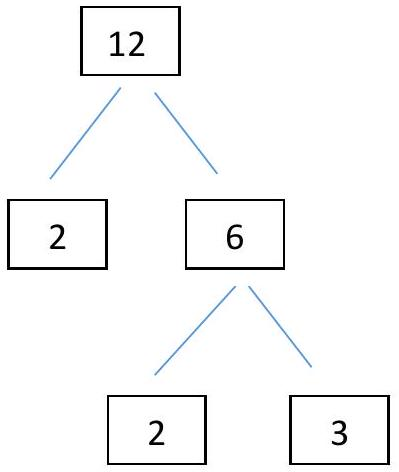
\includegraphics[max width=\textwidth, center]{2025_04_17_46e04c6acd873ea9558dg-119}
\end{enumerate}

Folosind aceeași reprezentare, precizați câte frunze are arborele obținut pentru numărul 4800.\\
a) 10\\
b) 12\\
c) 9\\
d) 15\\
e) 6\\
f) 16\\
2. Precizați ce se va afișa în urma execuției următorului program?

\begin{verbatim}
Limbajul C++
#include <iostream>
using namespace std;
int
v[]={5,2,9,11,22,17},n=6;
int calcul(int n)
{int i,poz,max;
    max=v[0]; poz=0;
    for(i=1;i<n;i++)
        if(v[i]>max)
            {max=v[i]; poz=i;}
            return poz;}
int main()
{ cout<<v[calcul(n)];
    return 0; }
Limbajul C
#include <stdio.h>
int
v[]={5,2,9,11,22,17},n=6;
int calcul(int n)
{ int i,poz,max;
        max=v[0];poz=0;
            for(i=1;i<n;i++)
                if(v[i]>max)
            { max=v[i]; poz=i;}
            return poz; }
var n:integer;
        v:array[0..5] of
        integer=(5,2,9,11,22,17);
function
calcul(n:integer):integer;
var i,poz,max:integer;
begin
    max:=v[0]; poz:=0;
    for i:=1 to n-1 do
        if v[i]>max then
            begin
                    max:=v[i];
                    poz:=i;
                end;
        calcul:=poz;
end;
begin
n:=6;
write(v[calcul(n)]);
end.
\end{verbatim}

Limbajul Pascal

\begin{verbatim}
int main()
{printf("%d",v[calcul(n)]);
    return 0; }
\end{verbatim}

a) Programul nu va afișa nimic, va genera eroare de compilare deoarece apelul de funcții nu este permis ca indice într-un tablou unidimensional.\\
b) 22\\
c) 17\\
d) 2\\
e) 11\\
f) 9\\
3. Pentru care dintre următoarele apeluri funcția f va returna valoarea 1 ?

\begin{verbatim}
Limbajul C/C++
int f(int n)
{
    int m=0,n1=n;
    while(n!=0)
    { m=m*10+n%10;
        n=n/10;
    }
    if(m==n1) return 1;
    else return 0;
}
\end{verbatim}

\begin{verbatim}
Limbajul Pascal
function f(n:integer):integer;
var m,n1:integer;
begin
    m:=0; n1:=n;
    while n<>0 do
    begin
        m:=m*10+n mod 10; n:=n div 10;
    end;
    if m=n1 then f:=1
        else f:=0; end;
\end{verbatim}

a) $f(123)$\\
b) $f(24)$\\
c) $\mathbf{f}$ (2112)\\
d) $f(17)$\\
e) $f(75)$\\
f) $f(1592)$\\
4. Într-un plan cartezian se găsesc 8 roboți dați prin coordonatele lor. Coordonatele celor 8 roboți sunt: $(2,2),(2,4),(2,6),(2,8),(4,2),(6,2),(6,-2)$, $(-2,-2)$. Doi roboți A și B se numesc vecini dacă se găsesc pe o paralelă la axele de coordonate și nu există un robot C situat între A și B pe aceeași paralelă. Ținând cont de regulile de mai sus, construiți un graf neorientat cu 8 noduri. Nodurile grafului sunt numerotate în ordinea coordonatelor (nodul 1 are coordonatele $(2,2)$, nodul 2 coordonatele $(2,4)$ ș.a.m.d.). Dacă robotul 1 este vecin cu robotul 2 atunci va exista muchie de la 1 la 2 în graf.\\
Precizați care dintre următoarele afirmații despre graful astfel obținut este adevărată?\\
a) Graful\\
b) Graful\\
c) Graful\\
d) Graful\\
e) Graful\\
f) Graful este este este este conține două conține trei eulerian. hamiltonian. complet. aciclic. componente componente conexe. conexe.\\
5. Corectați secvența de program de mai jos astfel încât ea să reprezinte calculul corect al valorii polinomului $P(x)=a_{0}+a_{1} x+a_{2} x^{2}+\ldots+a_{n} x^{n}$ într-un punct $c$ dat.

\begin{verbatim}
Limbajul C/C++
p=0;
for(i=0;i<=n;i++)
    p=p*c+a[i];
\end{verbatim}

Limbajul C/C++\\
a) Instrucțiunea $p=p * c+a[i]$; trebuie

\begin{verbatim}
Limbajul Pascal
p:=0;
for i:=0 to n do
    p:=p*c+a[i];
\end{verbatim}

Limbajul Pascal

\begin{verbatim}
înlocuită cu p=p*a[i]+c;
b) Instrucțiunea for(i=0;i<=n;i++)
trebuie înlocuită cu
for(i=n;i>=0;i--)
c) Instrucțiunea p=p*c+a [i];
trebuie înlocuită cu p=c*a [i]+p;
d) Variabila p trebuie inițializată cu -1.
e) Variabila p trebuie inițializată cu 1.
f) Instrucțiunea for(i=0;i<=n;i++)
trebuie înlocuită cu
for(i=1;i<=n;i++)
\end{verbatim}

a) Instrucțiunea $p:=p * c+a[i]$; trebuie înlocuită cu p:=p\textit{a[i]+c;\\
b) Instrucțiunea for $\mathrm{i}:=0$ to n do trebuie înlocuită cu\\
for i:=n downto 0 do\\
c) Instrucțiunea $p:=p * c+a[i]$; trebuie înlocuită cu\\
p:=c}a[i]+p;\\
d) Variabila $p$ trebuie inițializată cu -1.\\
e) Variabila $p$ trebuie inițializată cu 1.\\
f) Instrucțiunea for i:=0 to n do trebuie înlocuită cu\\
for i:=1 to n do\\
6. Precizați ce se va afișa pe ecran în urma execuției următorului program?

\begin{verbatim}
Limbajul C++
#include <iostream>
using namespace std;
int i;
int g(int i)
{ return i+3; }
int f(int i)
{ return i+g(i); }
int main()
{ i=3;
    cout<<i+f(g(i));
    return 0; }
\end{verbatim}

\begin{verbatim}
Limbajul Pascal
var i:integer;
function g(i:integer):integer;
begin
    g:=i+3;
end;
function f(i:integer):integer;
begin
    f:=i+g(i);
end;
begin
    i:=3; write(i+f(g(i))); end.
\end{verbatim}

\begin{verbatim}
Limbajul C
#include <stdio.h>
int i;
int g(int i)
{ return i+3; }
int f(int i)
{ return i+g(i); }
int main()
{ i=3; printf("%d",i+f(g(i))); return 0; }
\end{verbatim}

a) 18\\
b) 6\\
c) 15\\
d) 0\\
e) 9\\
f) 12\\
7. Precizați care dintre următoarele șiruri de numere poate reprezenta șirul gradelor nodurilor unui graf neorientat cu 7 noduri?\\
a) $(1,1,0,1,2,1,6)$\\
b) $(1,1,1,2,2,5,6)$\\
C) $(1,1,1,1,2,1,6)$\\
d) $(3,3,3,3,3,3,6)$\\
e) $(1,2,0,0,2,1,5)$\\
f) $(0,0,0,1,1,2,3)$\\
8. Robotul Robi se află într-un plan cartezian și are în jurul lui un grup de n roboți. El "mănâncă" robotul cel mai apropiat din grupul de roboți. Atât robotul Robi cât și ceilalți\\
roboți sunt identificați prin coordonatele lor. Datele de intrare se citesc de la tastatură astfel: n, numărul roboților din grup, apoi coordonatele robotului Robi și în continuare coordonatele celor n roboți. Corectați programul de mai jos astfel încât să afișeze corect coordonatele robotului care va fi "mâncat". În cazul în care există mai mulți roboți la aceeași distanță față de Robi, este mâncat primul robot întâlnit la distanța respectivă.

\begin{verbatim}
Limbajul C++
#include <iostream>
#include <cmath>
using namespace std;
struct robot{
    float x,y;
    };
float distanta (robot r1,
                    robot r2)
{
        return sqrt((r1.x-r2.x)*
            (r1.x-r2.x)+
            (r1.y-r2.y)*(r1.y-
r2.y));
}
int gaseste(robot robi,
robot a[], int n)
{
        float min,d;
        int i,poz;
        min=distanta(robi,a[0]);
        poz=1;
        for(i=1;i<n;i++)
        {
d=distanta(robi,a[i]);
            if(d<min){
                min=d;
                poz=i;
            }
        }
    return poz;
}
int main()
{ int n,i,k;
        robot robi,a[21];
        cin>>n;
        cin>>robi.x>>robi.y;
        for(i=0;i<n;i++)
            cin>>a[i].x>>a[i].y;
        k=gaseste(robi,a,n);
\end{verbatim}

\begin{verbatim}
Limbajul Pascal
type robot=record
                x,y:real;
            end;
            vector=array[0..20] of
robot;
var a:vector;
            robi:robot;
            n,i,k:integer;
function
distanta(r1,r2:robot):real;
begin
        distanta:=
    sqrt((r1.x-r2.x)*(r1.x-
r2.x) +
                    (r1.y-r2.y)*(r1.y-
r2.y));
end;
function gaseste(robi:robot;
a:vector;n:integer):integer;
var min,d:real;
            i,poz:integer;
begin
    min:=distanta(robi,a[0]);
    poz:=1;
    for i:=1 to n-1 do
    begin
            d:=distanta(robi,a[i]);
            if d<min then
                    begin
                        min:=d;
                            poz:=i;
                        end;
        end;
    gaseste:=poz;
end;
begin
    read(n);
    read(robi.x,robi.y);
    for i:=0 to n-1 do
            readln(a[i].x,a[i].y);
\end{verbatim}

\begin{verbatim}
        cout<<a[k].x<<"
"<<a[k].y;
        return 0;
}
Limbajul C
#include <stdio.h>
#include <math.h>
typedef struct {
        float x,y;
        } robot;
float distanta (robot r1, robot r2)
{
        return sqrt((r1.x-r2.x)*
            (r1.x-r2.x)+
            (r1.Y-r2.y)*(r1.Y-r2.y));
}
int gaseste(robot robi,
            robot a[],int n)
{
                float min,d;
                int i,poz;
                min=distanta(robi,a[0]);
                poz=1;
                for(i=1;i<n;i++)
                {
                        d=distanta(robi,a[i]);
                    if(d<min) {
                        min=d;
                        poz=i;
                    }
                }
        return poz;
}
int main()
{
    int n,i,k;
    robot robi,a[21];
    scanf("%d",&n) ;
    scanf("%f %f",&robi.x,&robi.y);
    for(i=0;i<n;i++)
            scanf("%f %f", &a[i].x, &a[i].y);
    k=gaseste(robi,a,n) ;
    printf("%f %f",a[k].x,a[k].y);
    return 0;}
\end{verbatim}

\section*{Limbajul C++}
a) Instrucțiunea if (d<min) trebuie înlocuită cu if (d>min)\\
b) Instrucțiunea min=d; trebuie înlocuită cu $d=m i n$;\\[0pt]
c) Instrucțiunea min=distanta (robi,a[0]); trebuie înlocuită cu

\begin{verbatim}
min=distanta(robi,a[1]);
\end{verbatim}

d) Instrucțiunea $\mathbf{p o z = 1}$; trebuie înlocuită cu $\mathbf{p o z = 0 ; ~}$\\
e) Secvența de instrucțiuni

\begin{verbatim}
for(i=0;i<n;i++) scanf("%f%f",&a[i].x,&a[i].y);
\end{verbatim}

trebuie înlocuită cu

\begin{verbatim}
for(i=0;i<n;i++) scanf("%f%f",&a.x[i],&a.y[i]);
\end{verbatim}

f) Instrucțiunea poz=i; trebuie înlocuită cu i=poz;

\section*{Limbajul C}
a) Instrucțiunea if (d<min) trebuie înlocuită cu if (d>min)\\
b) Instrucțiunea min=d; trebuie înlocuită cu d=min;\\[0pt]
c) Instrucțiunea min=distanta (robi, a [0]) ; trebuie înlocuită cu min=distanta(robi,a[1]);\\
d) Instrucțiunea $\mathbf{p o z = 1}$; trebuie înlocuită cu $\mathbf{p o z = 0 ; ~}$\\
e) Secvența de instrucțiuni

\begin{verbatim}
for(i=0;i<n;i++) cin>>a[i].x>>a[i].y;
\end{verbatim}

trebuie înlocuită cu

\begin{verbatim}
for(i=0;i<n;i++) cin>>a.x[i]>>a.y[i];
\end{verbatim}

f) Instrucțiunea $\mathbf{p o z = i}$; trebuie înlocuită cu $i=p o z$;

\section*{Limbajul Pascal}
a) Instrucțiunea if $d<m i n$ then trebuie înlocuită cu if $d>m i n$ then\\
b) Instrucțiunea $\min :=d$; trebuie înlocuită cu $\mathrm{d}:=\mathrm{min}$;\\[0pt]
c) Instrucțiunea min:=distanta (robi,a[0]) ; trebuie înlocuită cu

\begin{verbatim}
min:=distanta(robi,a[1]);
\end{verbatim}

d) Instrucțiunea poz:=1; trebuie înlocuită cu poz:=0;\\
e) Secvența de instrucțiuni\\[0pt]
for i:=0 to n-1 do readln(a[i].x, a[i].y);\\
trebuie înlocuită cu\\
for $i:=0$ to $n-1$ do readln(a.x[i], a.y[i]);\\
f) Instrucțiunea poz:=i; trebuie înlocuită cu i:=poz;\\
9. Precizați ce se va afișa pe ecran în urma execuției următorului program?

\begin{verbatim}
Limbajul C++
\#include <iostream>
using namespace std;
int $f()$
\{cout<<1<<" ";
    return 3; \}
int main()
\{ int s=0,i;
for (i=1;i<=f();i++)
\end{verbatim}

\begin{verbatim}
Limbajul C
#include <stdio.h>
int f()
{ printf("1 ");
    return 3; }
int main()
{ int s=0,i;
for(i=1;i<=f();i++)
        s=s+i;
\end{verbatim}

\begin{verbatim}
Limbajul Pascal
var s,i:integer;
function f:integer;
begin
    write('1 ');f:=3;
end;
begin
s:=0;
for i:=1 to f do
\end{verbatim}

\begin{center}
\begin{tabular}{|l|l|l|}
\hline
$s=s+i ;$ cout<<s; return 0;\} & printf("\%d",s); return 0; \} & s:=s+i; writeln(s) ;end. \\
\hline
Limbajul C++ & Limbajul C & Limbajul Pascal \\
\hline
a) Programul nu va afișa nimic, va genera eroare de compilare deoarece nu este permis apelul unei funcții ca valoare finală a contorului. & a) Programul nu va afișa nimic, va genera eroare de compilare deoarece nu este permis apelul unei funcții ca valoare finală a contorului. & a) Programul nu va afișa nimic, va genera eroare de compilare deoarece nu este permis apelul unei funcții ca valoare finală a contorului. \\
\hline
b) 11116 & b) 111116 & b) 16 \\
\hline
c) 1116 & c) 1116 & c) 1116 \\
\hline
d) 116 & d) 116 & d) 116 \\
\hline
e) 110 & e) 110 & e) 110 \\
\hline
f) 10 & f) 10 & f) 10 \\
\hline
\end{tabular}
\end{center}

\begin{enumerate}
  \setcounter{enumi}{9}
  \item Ce se va afișa pe ecran în urma execuției următorului program dacă de la tastatură se citește cuvântul caiet?
\end{enumerate}

\begin{verbatim}
Limbajul C++
#include <iostream>
#include <string.h>
using namespace std;
int main()
{char a[255];
int i,j,l,n;
cin.get(a,255);i=0;
n=strlen(a);
while(i<n)
if(strchr("aeiou",a[i]))
    { for(l=1;l<=2;l++)
        { n++;
            for(j=n;j>i;j--)
                a[j]=a[j-1];
                    }
                a[i+1]='p';
                a[i+2]=a[i]; i=i+3;
                }
                else i++;
        cout<<a; return 0; }
\end{verbatim}

\begin{verbatim}
Limbajul Pascal
var a:string[255];
        i,j,l,n:integer;
begin
    readln(a); i:=1;
    n:=length(a);
    while i<=n do
if pos(a[i],'aeiou')<>0 then
        begin
            for l:=1 to 2 do
                begin
                    n:=n+1;
                for j:=n downto i+1 do
                        a[j]:=a[j-1];
                        end;
        a[i+1]:='p';a[i+2]:=a[i];
        i:=i+3; end
    else i:=i+1;
for i:=1 to n do
        write(a[i]);
end.
\end{verbatim}

\begin{verbatim}
Limbajul C
#include <stdio.h>
#include <string.h>
int main()
{ char a[255];
    int i,j,l,n;
    scanf("%s",a); i=0; n=strlen(a);
    while(i<n)
        if(strchr("aeiou",a[i]))
        {
            for(l=1;l<=2;l++)
            {
                n++;
                for(j=n;j>i;j--)
                    a[j]=a[j-1];
            }
            a[i+1]='p'; a[i+2]=a[i]; i=i+3;
        }
        else i++;
    printf("%s",a); return 0;
}
\end{verbatim}

a) cpapipet\\
b) $c t$\\
c) cpcapaipiepetpt\\
d) capaipiepet\\
e) tepeipiapac\\
f) pcpaieptp\\
11. Ce va afișa următoarea funcție la apelul $f(30)$ ?

\begin{verbatim}
Limbajul C/C++
int f(int n)
{
    if(n>50) return n-5;
    else
        return f(f(n+7));
}
\end{verbatim}

\begin{verbatim}
Limbajul Pascal
function f(n:integer):integer;
begin
        if n>50 then
            f:=n-5
        else
            f:=f(f(n+7));
end;
\end{verbatim}

a) 47\\
b) 50\\
c) 150\\
d) 42\\
e) 44\\
f) 60\\
12. Fie $\mathbf{f}: \mathbf{A} \rightarrow \mathbf{B}$. Funcția $\mathbf{f}$ este injectivă dacă $\forall \mathbf{x}, \mathbf{y} \in \mathbf{A}, \mathbf{x} \neq \mathbf{y} \mathbf{f}(\mathbf{x}) \neq \boldsymbol{f}(\mathbf{y})$

\section*{Pentru funcția $\pounds:\{1,2,3\} \rightarrow\{1,2,3,4,5\}$, folosind metoda backtracking, primele trei funcții injective generate sunt:\\
x: 123\\
f(x): 123}
\section*{x: 123\\
f(x): 124}
x: 123\\
f(x): 125

Precizați care este a zecea funcție generată.\\
a) 543\\
b) 432\\
c) 213\\
d) 152\\
e) 145\\
f) 153\\
13. Numărul ciclurilor hamiltoniene distincte ale unui graf neorientat complet $\mathrm{G} \mathrm{cu} \mathrm{n} \geq 3$ noduri este egal cu\\
a) $n$\\
b) $\frac{(n-1)!}{2}$\\
c) n !\\
d) $\frac{n *(n-1)}{2}$\\
e) $\mathrm{n}^{*}(\mathrm{n}-1)$\\
f) $\frac{n}{2}$\\
14. Precizați ce se va afișa pe ecran în urma execuției următorului program?

\begin{verbatim}
Limbajul C++
#include <iostream>
using namespace std;
int v[]={15,12,7,20,-1,-5};
int f(int n)
{ cout<<n<<" ";
        if(n==0) return 0;
    else
    return
        v[n-1]<v[n] || f(n-1);
}
int main()
{ cout<<f(5); return 0; }
\end{verbatim}

\begin{verbatim}
Limbajul Pascal
var v:array[0..5] of
integer=(15,12,7,20,-1,-5);
function
f(n:integer):boolean;
begin
    write(n,' ');
    if n=0 then f:=false
    else f:=(v[n-1]<v[n]) or
f(n-1);
end;
begin
        write(f(5));
end.
\end{verbatim}

\begin{verbatim}
Limbajul C
\#include <stdio.h>
int $v[]=\{15,12,7,20,-1,-5\}$;
int $f($ int $n)$
\{
    printf("%d ",n);
    if(n==0) return 0;
    else return v[n-1]<v[n] || f(n-1);
}
int main()
{ printf("%d",f(5)); return 0; }
Limbajul C Limbajul C++
\end{verbatim}

a) 543210\\
b) 5432101\\
a) 543210\\
b) 5432101\\
c) 543\\
c) 543\\
d) 5431\\
e) 431\\
f) 54300\\
d) 5431\\
e) 431\\
f) 54300

Limbajul Pascal\\
a) 54321 false\\
b) 543210 true\\
c) 543\\
d) 543 true\\
e) 43 true\\
f) 5430 false\\
15. Dorim să decriptăm un cuvânt scris cu litere mari astfel: fiecare literă este codificată prin codul ei din care se scade un număr $\mathbf{k}(\mathbf{k}>=0)$. Numărul $\mathbf{k}$ se numește cheie de decriptare. De exemplu, dacă avem litera $\mathbf{I}$ și $\mathbf{k}$ este $\mathbf{6}$, vom obține după decriptare litera C. Vom considera literele așezate pe un cerc, după $\mathbf{Z}$ vine $\mathbf{A}$. Presupunem că șirul inițial este\\
reținut în variabila sir iar rezultatul obținut în urma decriptării tot în variabila sir. Considerând prima parte a programului cea de mai jos, care dintre următoarele secvențe realizează decriptarea corectă a unui șir de caractere citit de la tastatură cu o cheie k citită de la tastatură?

\begin{verbatim}
Limbajul C++
char sir[255];
int d;
unsigned int k,i;
cin>>sir;
cin>>k;
\end{verbatim}

Limbajul C++/C

\begin{verbatim}
Limbajul C
char sir[255];
int d;
unsigned int k,i;
scanf("%s",sir);
scanf("%u",&k);
\end{verbatim}

\begin{verbatim}
Limbajul Pascal
var sir:string;
    d:integer;
    i,k:word;
begin
    read(sir);
    read(k);
\end{verbatim}

\begin{verbatim}
a) d = 'Z'-'A';
    for(i=0;i<strlen(sir);i++)
            sir[i]='A'+(sir[i]-'A'+d)%('Z'-'A'+1);
b) d = k;
    for(i=0;i<strlen(sir);i++)
        sir[i]='A'+(sir[i]-'A'+d)%('Z'-'A'+1);
c) d = 'Z'-'A'+1-k;
    for(i=0;i<strlen(sir);i++)
        sir[i]='A'+(sir[i]-'A'-d)%('Z'-'A'+1);
d) d = 'Z'-'A'+1-k;
    for(i=0;i<strlen(sir);i++)
        sir[i]='A'+(sir[i]-'A'+d)%('Z'-'A'+1);
e) d = k;
    for(i=0;i<strlen(sir);i++)
        sir[i]='A'+(sir[i]-'A'+d)%('Z'-'A'+26);
f) d = 'Z'-'A';
    for(i=0;i<strlen(sir);i++)
        sir[i]='A'+(sir[i]-'A'+d)%('Z'-'A'-25);
\end{verbatim}

\section*{Limbajul Pascal}
a) d:=ord('Z')-ord('A');\\[0pt]
for i:=1 to length(sir) do sir[i]:=chr(ord('A')+(ord(sir[i])- ord('A')+d ) mod

\begin{verbatim}
(ord('Z')-ord('A')+1));
\end{verbatim}

b) $\mathrm{d}:=\mathrm{k}$;\\
for $i:=1$ to length(sir) do\\[0pt]
sir[i]:=chr(ord('A')+(ord(sir[i])-ord('A')-d) mod\\
(ord('Z')-ord('A')+1));\\
c) $d:=o r d(' Z ')-o r d(' A ')+1-k ;$\\
for i:=1 to length(sir) do\\[0pt]
sir[i]:=chr(ord('A')+(ord(sir[i])-ord('A')-d) mod\\
(ord('Z')-ord('A')+1)) ;\\
d) $d:=o r d(' Z ')-o r d(' A ')+1-k ;$\\
for i:=1 to length(sir) do

\begin{verbatim}
        sir[i]:=chr(ord('A')+(ord(sir[i])-ord('A')+d) mod
    (ord('Z')-ord('A')+1)) ;
e) d:=k;
    for i:=1 to length(sir) do
    sir[i]:=chr(ord('A')+(ord(sir[i])-ord('A')-d) mod
    (ord('Z')-ord('A')+26)) ;
f) d:=ord('Z')-ord('A');
    for i:=1 to length(sir) do
    sir[i]:=chr(ord('A')+(ord(sir[i])-ord('A')+d)mod
(ord('Z')-ord('A')-25)) ;
\end{verbatim}

\section*{Varianta 23}
\begin{enumerate}
  \item Trei variabile de tip întreg au valorile $a=13, b=5, c=3$. Dintre expresiile următoare, cea care are valoarea 1 ( $\mathrm{C}++/ \mathrm{C}$ ) respectiv true (Pascal) este:\\
Limbajul C++/C\\
a) $a / c * 2<5+c * 4 \% 5$\\
b) $c \% b=a \% c$\\
c) $b+a / 10!=b \% c * a / c$\\
d) $(b>c) \& \&!(b * c \% 7==2 * a-b * b)$\\
e) $c \% b * 10<a * 2$\\
f) $c / b * b / c==1$
\end{enumerate}

Limbajul Pascal\\
a) a div $c * 2<(5+c * 4 \bmod 5)$\\
b) $c \bmod b=a \bmod c$\\
c) $b+a \operatorname{div} 10<>b \bmod c * a \operatorname{div} c$\\
d) $(b>c)$ and $\operatorname{not}((b * c \bmod 7)=(2 * a-b * b))$\\
e) $c \bmod b * 10<a * 2$\\
f) $c \operatorname{div} b * b \operatorname{div} c=1$\\
2. Într-un graf neorientat cu 13 noduri, fiecare nod are gradul d. Valoarea lui d nu poate fi:\\
a) 2\\
b) 4\\
c) 6\\
d) 8\\
e) 10\\
f) 11\\
3. Variabila i este de tip întreg. Numărul total al atribuirilor care se execută în urma rulării secvenței următoare este:

\begin{verbatim}
Limbajul C++/C
i=1;
while(i*i<2020)
    i=i*2;
\end{verbatim}

a) 5\\
b) 6\\
c) 7\\
d) 9\\
e) 11\\
f) 12\\
4. Considerând că variabila spoate reține un șir cu cel mult 100 de caractere și variabila i este de tip întreg, în urma executării următoarei secvențe de instrucțiuni, lungimea efectivă a șirului s este:

\begin{verbatim}
Limbajul C++/C
strcpy(s,"2020+2020=4040");
for(i=0;i<strlen(s);i++)
if(strchr("0123456789",s[i]))
    strcpy(s+i,s+i+1);
\end{verbatim}

a) 0\\
b) 2\\
c) 5\\
d) 6\\
e) 8\\
f) 11\\
5. Pentru a verifica dacă elementele unui tablou unidimensional cu $\mathbf{n}$ elemente numere întregi sunt distincte două câte două, numărul de comparații executate este:\\
a) $2 n$\\
b) $n(n-1) / 2$\\
c) $n(n-1)$\\
d) $(n-1)^{2}$\\
e) $n^{2}$\\
f) $n$ !\\
6. În urma executării următoarei secvențe de program, variabila $\mathbf{x}$, de tip întreg, va avea valoarea:

\begin{verbatim}
Limbajul C++/C
x=15;
x=x*3/4*4/3;
do {if(x%2==0) x=x/2;
        else x=x-5;
    }while(x>0);
\end{verbatim}

\begin{verbatim}
Limbajul Pascal
x:=15;
x:=x*3 div 4*4 div 3;
repeat
if x mod 2=0 then x:=x div 2
else x:=x-5;
until x<=0;
\end{verbatim}

a) -6\\
b) -5\\
c) $\mathbf{- 4}$\\
d) 0\\
e) 2\\
f) 5\\
7. Utilizând un algoritm backtracking se generează în ordine crescătoare toate numerele naturale cu patru cifre care au suma cifrelor egală cu 4. Primele trei soluții sunt: 1003, 1012, 1021. În șirul generat, numărul 2020 ocupă poziția:\\
a) 10\\
b) 11\\
c) 12\\
d) 13\\
e) 14\\
f) 15\\
8. Dacă $\mathbf{s}, \mathbf{i}, \mathbf{j}, \mathbf{n}$ sunt variabile de tip întreg și a este un tablou bidimensional cu $\mathbf{n}$ linii și n coloane numerotate de la 1 la n, următorul algoritm calculează:

\begin{verbatim}
Limbajul C++/C
s=0;
for(i=1;i<=n;i++)
    for(j=1;j<i;j++)
        s=s+a[i][j];
\end{verbatim}

\begin{verbatim}
Limbajul Pascal
s:=0;
for i:=1 to n do
    for j:=1 to i-1 do
        s:=s+a[i,j];
\end{verbatim}

a) suma elementelor de sub diagonala principală exclusiv elementele diagonalei principale\\
b) suma elementelor de sub diagonala secundară exclusiv elementele diagonalei secundare\\
c) numărul elementelor de deasupra diagonalei principale inclusiv elementele diagonalei principale\\
d) suma elementelor de pe diagonala principală\\
e) suma elementelor de sub diagonala principală inclusiv elementele diagonalei principale\\
f) suma elementelor de deasupra diagonalei secundare inclusiv elementele diagonalei secundare\\
9. Se consideră următoarele declarații de tipuri și variabile:

\begin{verbatim}
Limbajul C++
struct a
    { int b;
        char c[10];
    };
struct d
    { char e[10];
        float f;
        a g;
\end{verbatim}

\begin{verbatim}
Limbajul Pascal
type a=record
    b:integer;
    c:string[10]
end;
    d=record
        e: string[10];
        f: real;
        g:a
\end{verbatim}

\begin{verbatim}
    } h;
Limbajul C
typedef struct
    { int b;
        char c[10];
    }a;
typedef struct
    { char e[10];
        float f;
        a g;
    }d;
d h;
\end{verbatim}

\begin{verbatim}
end;
var h:d;
\end{verbatim}

Dintre următoarele expresii, de tip caracter este:\\[0pt]
a) g.e[2]\\
b) h.a.c\\[0pt]
c) h.a.c[0]\\[0pt]
d) h.c [2]\\[0pt]
e) h.g.c [2]\\[0pt]
f)d.e[2]\\
10. Se consideră un arbore cu 8 noduri și muchiile $[1,2]$, $[2,3]$, $[3,6],[4,3]$, $[5,7],[7,2],[8,2]$. Pentru ca arborele să conțină un număr maxim de lanțuri elementare de lungime 3 care nu conțin rădăcina, se poate alege ca rădăcină oricare dintre nodurile:\\
a) $1,2,4,5$\\
b) $1,2,5,6$\\
c) $1,3,6,7$\\
d) $2,3,4,5,6$\\
e) $1,4,5,6,8$\\
f) $2,3,4,7,8$\\
11. În urma executării următoarei secvențe de program tabloul unidimensional a, cu 6 elemente numerotate de la 1 la 6, va conține valorile:

\begin{verbatim}
Limbajul C++/C
for (i=1;i<=6;i++)
    if (i%2!=0) a[i]=i/2;
    else a[i]=7-i;
for(i=6;i>=3;i--)
    a[a[i]]=2*i%7;
\end{verbatim}

\begin{verbatim}
Limbajul Pascal
for i:=1 to 6 do
if i mod 2<>0 then a[i]:=i div 2
else a[i]:=7-i;
for i:=6 downto 3 do
a[a[i]]:=2*i mod 7;
\end{verbatim}

a) 056135\\
b) 531321\\
c) 636223\\
d) 615263\\
e) 631221\\
f) 631321\\
12. Pentru apelul $\mathbf{s}(\mathbf{2 0 2 0}, \mathbf{2})$ al subprogramului de mai jos, enunțul adevărat este:

\begin{verbatim}
Limbajul C++/C
int s(int n, int d)
{
    if(n==1) return 0;
    if (n%d==0)
        return 1+s(n/d,d);
    else
        return s(n,d+1);
}
\end{verbatim}

\begin{verbatim}
Limbajul Pascal
function s(n,d:integer): integer;
begin
if n=1 then
        s:=0
else if n mod d=0 then
            s:=1+s(n div d,d)
    else s:=s(n,d+1)
end;
\end{verbatim}

a) $s(2020,2)=3$ și reprezintă numărul divizorilor primi ai numărului 2020\\
b) $s(2020,2)=4$ și reprezintă numărul divizorilor primi ai numărului 2020\\
c) $\mathbf{s}(\mathbf{2 0 2 0}, \mathbf{2})=\mathbf{4}$ și reprezintă suma exponenților divizorilor primi din descompunerea în factori primi a numărului 2020\\
d) $\mathbf{s}(\mathbf{2 0 2 0}, \mathbf{2})=6$ și reprezintă suma exponenților divizorilor primi din descompunerea în factori primi a numărului 2020\\
e) $s(2020,2)=10$ și reprezintă numărul divizorilor proprii ai numărului 2020\\
f) $s(2020,2)=12$ și reprezintă numărul divizorilor numărului 2020\\
13. Numărul de grafuri neorientate cu șase noduri, în care nodul $\mathbf{1}$ are gradul 1 și nodul 2 are gradul 2 este:\\
a) 92\\
b) 1280\\
c) 1536\\
d) 1792\\
e) 1920\\
f) 2560\\
14. În urma rulării programului următor vor fi afișate valorile:

\begin{verbatim}
Limbajul C++
#include <iostream>
using namespace std;
void f (int &a, int b)
{ int x=3;
    a--;
    b++;
    x--;
    cout<<<a<<' '<<<b<<' '<<<x<<' ';
}
int main()
{ int i, x=4, y=6;
    for(i=1;i<=3;i++)
        f(x,x+y) ;
    cout<<x<<<' '<<y ;
        return 0;
}
\end{verbatim}

Limbajul Pascal\\
program main;\\
var $x, y, i: i n t e g e r ;$\\
procedure $f$ (var a: integer; b:integer);\\
var x:integer;\\
begin\\
x:=3;\\
$\operatorname{dec}(a)$; inc (b) ; $\operatorname{dec}(x)$;\\
write (a,' ',b,' ', x,' ');\\
end;\\
begin\\
x:=4;\\
$\mathrm{y}:=6$;\\
for i:=1 to 3 do\\
$\mathrm{f}(\mathrm{x}, \mathrm{x}+\mathrm{y})$;\\
write ( x, ' $\quad$, y )\\
end.\\
a) 311236\\
b) 311246\\
$\begin{array}{llllllllllllllllllllll}\text { c) } 3 & 11 & 3 & 2 & 10 & 2 & 1 & 9 & 1 & 1 & 6 & \text { d) } 2 & 11 & 2 & 0 & 9 & 0 & -2 & 7 & -2 & -2 & 6 \\ \text { e) } 3 & 11 & 2 & 3 & 11 & 2 & 3 & 11 & 2 & 4 & 6 & \text { f) } 3 & 11 & 2 & 2 & 10 & 2 & 1 & 9 & 2 & 1 & 6\end{array}$\\
15. Se sortează crescător tabloul v=(3, 4, 2, 5, 1, 7, 6). O propoziție falsă este:\\
a) Sortând prin metoda Bubble Sort se fac $\mathbf{7}$ interschimbări.\\
b) Aplicând metoda de sortare prin interclasare numerele 1 și 4 nu se compară.\\
c) Aplicând metoda de sortare prin selecție se execută cel mult 6 interschimbări.\\
d) Sortând prin selecția minimului, numerele 2 și 3 se compară de două ori.\\
e) Aplicând metoda de sortare Bubble Sort se poate obține ca etapă intermediară tabloul $\mathrm{v}=(3,2,4,1,5,6,7)$.\\
f) Aplicând metoda de sortare prin inserție se poate obține ca etapă intermediară tabloul $\mathrm{v}=(1,3,4,2,5,7,6)$.

\section*{Varianta 24}
\begin{enumerate}
  \item Expresia de mai jos are valoarea $\mathbf{1}(\mathrm{C}++/ \mathrm{C})$ respectiv true (Pascal) dacă și numai dacă n este:
\end{enumerate}

Limbajul C++/C\\
$\mathrm{n} \% 2==1 \& \& \mathrm{n}$ * $\mathrm{n}<100$

Limbajul Pascal\\
( $\mathrm{n} \bmod 2=1$ ) and ( $\mathrm{n} * \mathrm{n}<100$ )\\
a) număr întreg impar mai mic decât 10\\
b) număr întreg impar, din intervalul $(-10,10)$\\
c) număr natural mai mic decât 100\\
d) număr natural impar de o singură cifră\\
e) număr întreg par mai mic decât 10\\
f) număr natural impar cu cel mult două cifre\\
2. Dacă a este un tablou bidimensional cu $\mathbf{n}$ linii și $\mathbf{n}$ coloane, numerotate de la $\mathbf{1}$ la $\mathbf{n}$, elementul de pe linia i și coloana $\mathbf{j}$ se află pe diagonala secundară dacă între indici există relația:\\
a) $i<j$\\
b) $i>j$\\
c) $i=j$\\
d) $i+j=n-1$\\
e) $i+j=n$\\
f) $i+j=n+1$\\
3. Graful neorientat complet $\mathbf{G}$ are $\mathbf{1 0}$ noduri. Un enunț adevărat este:\\
a) G este arbore\\
b) G are 50 de muchii\\
c) $\mathbf{G}$ nu este graf hamiltonian și nici eulerian\\
d) $G$ este graf hamiltonian dar nu eulerian\\
e) $\mathbf{G}$ nu este graf hamiltonian dar este graf eulerian\\
f) G este graf hamiltonian și eulerian\\
4. Se consideră că $\mathbf{d}, \mathbf{i}, \mathbf{k}, \mathbf{n}$ sunt variabile de tip întreg și a este un tablou unidimensional cu n numere întregi numerotate de la 1 la $n$. La finalul execuției secvenței următoare, variabila $\mathbf{k}$ are valoarea $\mathbf{1}$ dacă și numai dacă elementele tabloului a formează o progresie aritmetică. Expresia corectă care completează punctele de suspensie este:

\begin{verbatim}
Limbajul C++/C
k=1;
d=a[2]-a[1];
for(i=3;i<=n;i++)
    if ( . . . . )
        k=0;
\end{verbatim}

\begin{verbatim}
Limbajul Pascal
k:=1;
d:=a[2]-a[1];
for i:=3 to n do
    if . . . . then
        k:=0;
\end{verbatim}

Limbajul C++/C\\
a) $a[i+1]-a[i]!=d$\\
b) $a[i]-a[i+1]!=d$\\
c) $\mathrm{a}[\mathrm{i}]-\mathrm{a}[\mathrm{i}-1]!=\mathrm{d}$\\
d) $a[i+1]-a[i]==d$\\
e) $a[i]+a[i+1]!=d$\\
f) $a[i]-a[i-1]==d$\\
Limbajul Pascal\\[0pt]
a) a[i+1]-a[i]<>d\\
b) $a[i]-a[i+1]<>d$\\
c) $a[i]-a[i-1]<>d$\\
d) $a[i+1]-a[i]=d$\\
e) $a[i]+a[i+1]<>d$\\
f) $a[i]-a[i-1]=d$\\
5. Se consideră un arbore cu 8 noduri și muchiile $[1,2],[2,3],[3,6],[4,3],[5,7],[7,2]$, [8,2]. Înălțimea arborelui este egală cu lungimea celui mai lung lanț elementar care unește rădăcina de o frunză. Arborele dat are înălțime minimă dacă se va alege ca rădăcină nodul:\\
a) 1\\
b) 2\\
c) 3\\
d) 5\\
e) 7\\
f) 8\\
6. În urma execuției secvenței următoare, în care toate variabilele sunt de tip întreg, valoarea variabilei $\boldsymbol{n}$ este:

\begin{verbatim}
Limbajul C++/C
n=0; a=11357; b=1426; p=1;
    while(a!=b)
    { x=a%10;y=b%10;
            if(x<y) n=n+p*x;
            else n=n+p*y;
            p=p*10;a=a/10;b=b/10;
    }
\end{verbatim}

a) 1326\\
b) 1356\\
c) 6241\\
d) 11326\\
e) 11457\\
f) 62411

\begin{verbatim}
Limbajul Pascal
n:=0; a:=11357; b:=1426; p:=1;
while a<>b do begin
x:=a mod 10; y:=b mod 10;
if }x<y\mathrm{ then n:=n+p*x
else n:=n+p*y;
p:=p*10; a:=a div 10; b:=b
div 10
end;
\end{verbatim}

\begin{enumerate}
  \setcounter{enumi}{6}
  \item Fie enunțul: „pentru a sorta descrescător un tablou unidimensional cu 20 de elemente numere reale, utilizând metoda selecției, nu sunt necesare mai mult de $\mathbf{x}$ determinări ale valorii maxime". Enunțul este adevărat dacă $\mathbf{x}$ este egal cu:\\
a) 0\\
b) 10\\
c) 19\\
d) 20\\
e) 190
  \item Matricea alăturată este matricea de adiacență a unui graf:
\end{enumerate}

\begin{verbatim}
f) 400
\end{verbatim}

\begin{center}
\begin{tabular}{llll}
0 & 1 & 1 & 0 \\
1 & 0 & 1 & 0 \\
1 & 0 & 0 & 0 \\
0 & 1 & 0 & 0 \\
\end{tabular}
\end{center}

a) orientat cu 6 noduri și $\mathbf{3}$ arce\\
b) neorientat cu 4 noduri și 3 muchii\\
c) orientat cu 4 noduri și 6 arce\\
d) neorientat cu 6 noduri și 6 muchii\\
e) orientat cu $\mathbf{4}$ noduri și $\mathbf{3}$ arce\\
f) neorientat cu 4 noduri și 6 muchii\\
9. Utilizând un algoritm backtracking se generează în ordine lexicografică toate anagramele cuvântului roman. Soluția generată imediat înainte de cuvântul norma și soluția generată imediat după cuvântul norma sunt:\\
a) nramo și noram\\
b) nramo și nrmao\\
c) nomra și noram\\
d) nomra și nramo\\
e) noram și nramo\\
f) nomar și nramo\\
10. Variabilele $\mathbf{i}, \mathbf{j}, \mathbf{k}$ sunt de tip întreg iar $\mathbf{s}$ reține un șir de caractere format din litere mici și spații (cuvintele sunt despărțite printr-un singur spațiu). În urma executării următoarei secvențe de program, variabila $\mathbf{k}$ are valoarea $\mathbf{0}$ dacă șirul $\mathbf{s}$ este inițial:

\begin{verbatim}
Limbajul C++/C
for(i=0;i<strlen(s);i++)
    if(s[i]==' ')
        strcpy(s+i,s+i+1);
\end{verbatim}

\begin{verbatim}
Limbajul Pascal
for i:=1 to length(s) do
    if s[i]=' ' then
        delete(s,i,1);
\end{verbatim}

\begin{verbatim}
i=0;
j=strlen(s)-1;
k=1;
while(i<j)
    {
        if (s[i]!=s[j])
            k=0;
        i++;
        j--;
    }
\end{verbatim}

\begin{verbatim}
i:=1;
j:=length(s);
k:=1;
while i<j do
    begin
        if s[i]<>s[j] then
            k:=0;
        inc(i);
        dec(j)
end;
\end{verbatim}

a) atasata\\
b) o rama maro\\
c) o rama alba\\
d) elisa vasile\\
e) nora aron\\
f) vasile elisav\\
11. Dacă din programul principal se apelează $\mathbf{f}(\mathbf{f}(3))$, numărul de autoapeluri ale funcției $\mathbf{f}$, definită mai jos, este:

\begin{verbatim}
Limbajul C++/C
int f (int a)
{
    if (a<2)
        return 1;
    else
        return f(a-1)+2*f(a-3);
}
\end{verbatim}

a) 8\\
b) 9\\
c) 10\\
d) 14\\
e) 15\\
f) 16

\begin{verbatim}
Limbajul Pascal
function f(a:integer):integer;
begin
if a<2 then
    f:=1
else
    f:=f(a-1)+2*f(a-3)
end;
\end{verbatim}

\begin{enumerate}
  \setcounter{enumi}{11}
  \item Secvența de mai jos construiește tabloul bidimensional a cu n linii și n coloane, numerotate de la 1 la $\mathbf{n}$. Pentru $\mathbf{n = 4}$, suma elementelor de pe diagonala principală este:
\end{enumerate}

\begin{verbatim}
Limbajul C++/C
x=1;
y=1;
for(i=1;i<=n;i++)
    for(j=1;j<=n+1-i;j++)
        {
            a[i][j]=x;
            x++;
        }
for(j=n;j>=1;j--)
        for(i=n;i>=n+1-j;i--)
            {
                a[i][j]=y;
                y++;
            }
\end{verbatim}

\begin{verbatim}
Limbajul Pascal
x:=1;
y:=1;
for i:=1 to n do
    for j:=1 to n+1-i do
        begin
            a[i,j]:=x;
            inc(x)
        end;
for j:=n downto 1 do
    for i:=n downto n+1-j do
        begin
            a[i,j]:=y;
            inc(y)
        end;
\end{verbatim}

a) 9\\
b) 12\\
c) 14\\
d) 16\\
e) 28\\
f) 30\\
13. Pentru funcția dată mai jos, $\mathbf{f}(95)$ și $\mathbf{f}(59)$ au valorile:

\begin{verbatim}
Limbajul C++/C
int f (int x)
{
    if (x>=100)
\end{verbatim}

\begin{verbatim}
Limbajul Pascal
function f (x:integer) :
integer;
begin
\end{verbatim}

\begin{verbatim}
        return x+2;
    else
        return f (f(x+2)+1);
}
\end{verbatim}

\begin{verbatim}
    if x>=100 then
        f:=x+2
    else
        f:=f(f(x+2)+1)
end;
\end{verbatim}

a) 103 și 146\\
b) 109 și 162\\
c) 110 și 163\\
d) 103 și 163\\
e) 112 și 157\\
f) 112 și 166\\
14. Sortând crescător prin metoda selecției, cu număr minim de interschimbări (se interschimbă doar elemente distincte), tablourile unidimensionale $\mathbf{v}=(3,8,2,7)$, $\mathbf{x}=(4,5,1,7), \mathbf{y}=(4,7,9,6)$ și $\mathbf{z}=(6,3,2,9)$ se calculează numărul operațiilor (comparări și atribuiri) efectuate. Afirmația adevărată este:\\
a) Pentru v și y s-a realizat un număr egal de operații\\
b) Pentru v și $\mathbf{z}$-a realizat un număr egal de operații\\
c) Cel mai mare număr de operații s-a efectuat pentru $\mathbf{x}$\\
d) Cel mai mare număr de operații s-a efectuat pentru $\mathbf{y}$\\
e) Cel mai mic număr de operații $s$-a efectuat pentru $\mathbf{z}$\\
f) Cel mai mic număr de operații s-a efectuat pentru y\\
15. În urma executării secvenței de program de mai jos se afișează:

\begin{verbatim}
Limbajul C++/C
int f (int a, int b, int e)
{
        int x;
        if(a<2)
            return e+1;
        if(a%b==0)
        {
            if(e==0)
            cout<<b<<' ';
            tf("%d ",b);
            e++;
        return f(a/b,b,e);
    }
else
    {
        x=e+1;
        e=0;
        b++;
        return x*f(a,b,e);
    }
}
int main()
{ int x,y,e;
    cin>>x; |scanf("%d",&x);
    y=2;
    e=0;
    cout<<f(x,y,e);
|printf("%d",f(x,y,e));
\end{verbatim}

\begin{verbatim}
Limbajul Pascal
program p;
var x,y,e: integer;
function f(a,b,e:integer) :integer;
var x:integer;
begin
    if a<2 then
        f:=e+1
    else
        begin
            if a mod b=0 then
                begin
                    if e=0 then
                    write(b,' ');
                    inc(e);
                    f:=f(a div b,b,e)
                end
            else
                begin
                    x:=e+1;e:=0;inc(b) ;
                    f:=x*f(a,b,e)
                end
        end
end;
begin
        read(x) ;
        y:=2;
        e:=0;
        writeln(f(x,y,e))
\end{verbatim}

\}\\
|end.\\
a) divizorii proprii ai numărului $\mathbf{x}$\\
b) numărul de divizori proprii ai numărului $\mathbf{x}$\\
c) divizorii proprii și numărul divizorilor proprii ai numărului $\mathbf{x}$\\
d) divizorii primi ai lui $\mathbf{x}$ și numărul tuturor divizorilor lui $\mathbf{x}$\\
e) divizorii proprii ai numărului $\mathbf{x}$ și produsul exponenților divizorilor primi din descompunerea în factori primi a numărului $\mathbf{x}$\\
f) divizorii primi ai numărului $\mathbf{x}$ și produsul exponenților divizorilor primi din descompunerea în factori primi a numărului $\mathbf{x}$

\section*{Varianta 25}
\begin{enumerate}
  \item Se dă o variabilă a care reține un număr natural nenul. Care dintre următoarele expresii are valoarea $0 /$ false?\\
a) $C++/ C: a *(a+1) / 2<a * a+1$
\end{enumerate}

Pascal: a*(a+1) DIV 2<a\textit{a+1\\
b) C++/C: 4}a*(a-1)<a*a-2

Pascal: 4\textit{a} $(a-1)<a * a-2$\\
c) $C++/ C: a>0 \& \&(a \% 10+(a+1) \% 10)$

Pascal: $a>0$ AND (a MOD 10+(a+1) MOD 10)\\
d) $\mathrm{C}++/ \mathrm{C}: \mathbf{a} \% 2+(\mathrm{a}+1) \% 2==1$

Pascal: a MOD 2+(a+1) MOD $2=1$\\
e) $C++/ C:(a-1) *(a+1)>a * a-2$

Pascal: $(a-1)$ * $(a+1)>a * a-2$\\
f) C++/C: a* $(a+1)>=a * a+1$

Pascal: a* $(a+1)>=a * a+1$\\
2. În secvența de program variabilele $\mathbf{i}$ și $\mathbf{j}$ sunt de tip întreg iar $\mathbf{A}$ este un tablou bidimensional cu 5 linii și 5 coloane numerotate de al 0 la 4,\\
$\boldsymbol{A}=\left(\begin{array}{lllll}1 & 2 & 3 & 4 & \mathbf{5} \\ \mathbf{6} & \mathbf{7} & \mathbf{8} & 9 & \mathbf{0} \\ \mathbf{1} & 2 & 3 & 4 & \mathbf{5} \\ \mathbf{6} & \mathbf{7} & \mathbf{8} & 9 & \mathbf{0} \\ \mathbf{1} & 2 & 3 & 4 & 5\end{array}\right)$. În urma executării următoarelor instrucțiuni se va afiṣa:\\
Limbajul C++

\begin{verbatim}
i=4;
j=0;
cout<<A[i][j];
while(j!=4)
    {
        i--;
        cout<<A[i][j];
        j++;
        cout<<A[i][j];
    }
\end{verbatim}

\begin{verbatim}
Limbajul C
i=4;
j=0;
printf("%d",A[i][j]);
while(j!=4)
    {
        i--;
        printf("%d",A[i][j]);
        j++;
        printf("%d",A[i][j]);
    }
\end{verbatim}

Limbajul Pascal

\begin{verbatim}
i:=4;
j:=0;
write(A[i][j]);
while j<>4 do
    begin
        i:=i-1; write(A[i][j]);
        j:=j+1;
\end{verbatim}

\begin{verbatim}
    write(A[i][j])
end;
\end{verbatim}

a) 167238945\\
b) 127834905\\
c) 549832761\\
d) 509438721\\
e) 127850943\\
f) 509412783\\
3. Fie o coadă inițial vidă. Cu ajutorul subprogramelor $\mathbf{A d}(\mathbf{x})$ respectiv $\mathbf{E l}()$ este adăugat elementul $\mathbf{x}$ respectiv șters un element din coadă. Care va fi suma elementelor din coadă în urma executării operațiilor următoare?\\
Ad (3) El() Ad (7) Ad (9) El () Ad (5) Ad (2) El()\\
a) 12\\
b) 14\\
c) 10\\
d) 15\\
e) 7\\
f) 16\\
4. Fie $M=\left(\begin{array}{llllll}\mathbf{0} & \mathbf{0} & \mathbf{0} & \mathbf{1} & \mathbf{0} & \mathbf{1} \\ \mathbf{0} & \mathbf{0} & \mathbf{1} & \mathbf{0} & \mathbf{0} & \mathbf{0} \\ \mathbf{0} & \mathbf{1} & \mathbf{0} & \mathbf{0} & \mathbf{1} & \mathbf{0} \\ \mathbf{1} & \mathbf{0} & \mathbf{0} & \mathbf{0} & \mathbf{0} & \mathbf{0} \\ \mathbf{0} & \mathbf{0} & \mathbf{1} & \mathbf{0} & \mathbf{0} & \mathbf{0} \\ \mathbf{1} & \mathbf{0} & \mathbf{0} & \mathbf{0} & \mathbf{0} & \mathbf{0}\end{array}\right)$ matricea de adiacenṭă a unui graf neorientat $\mathbf{G}$.

Numărul de componente conexe ale grafului $\mathbf{G}$ este:\\
a) 0\\
b) 1\\
c) 2\\
d) 3\\
e) 4\\
f) 5\\
5. Numărul de noduri și numărul de frunze ale arborelui cu rădăcină memorat în următorul vector de tați ( $\mathbf{0}, \mathbf{1}, \mathbf{1}, \mathbf{2}, \mathbf{2}, \mathbf{3}, \mathbf{6}, \mathbf{7}, 7$ ) este:\\
a) 90\\
b) 95\\
c) 84\\
d) 12\\
e) $8 \quad 3$\\
f) $9 \quad 4$\\
6. Se dă mulțimea $A=\{1,2,3,4\}$. Un algoritm generează în ordine crescătoare, toate numerele naturale de $\mathbf{n}$ cifre, folosind cifre din mulțimea $\mathbf{A}$, numere care au suma cifrelor egală cu 6. Dacă pentru $n=3$, primele trei soluții generate sunt, în ordine, 114, 123, 132, numărul de ordine al soluției 312 este:\\
a) 4\\
b) 5\\
c) 6\\
d) 7\\
e) 8\\
f) 9\\
7. Variabila i memorează un număr natural, iar variabila a memorează șirul examen. În urma executării următoarelor instrucțiuni se va afișa:

\begin{verbatim}
Limbajul C++/C
for(i=0;i<5;i++)
    if(a[i]<a[i+1])
        a[i]=a[i+1];
cout<<a; | printf("%s",a);
\end{verbatim}

\begin{verbatim}
Limbajul Pascal
for i:=0 to 4 do
    if a[i]<a[i+1] then
        a[i]:=a[i+1];
write(a);
\end{verbatim}

a) $x \times m m n n$\\
b) exmmnn\\
c) $\mathfrak{f x b m f n}$\\
d) $\operatorname{exx} \times \mathrm{xn}$\\
e) xamenn\\
f) nemaxe\\
8. Fie subprogramul recursiv:

\begin{verbatim}
Limbajul C++/C
void numar(int n)
{
    if(n<=100)
\end{verbatim}

\begin{verbatim}
Limbajul Pascal
procedure numar(n: longint);
begin
    if n<=100 then
\end{verbatim}

\begin{verbatim}
        cout<<'\n';
        lprintf("\n");
    else
        {
            if(n%10<5)
                cout<<n%10;
                |printf("%d", n%10);
            numar(n/10) ;
            if(n%10>5)
                cout<<n%10;
            |printf("%d", n%10);
        }
}
\end{verbatim}

În urma apelului numar (824972345) se va afișa:\\
b) 4324\\
c) 4234\\
d) 4234\\
e) 3244 79 97\\
97 97\\
f) 2443 97\\
f) 2443 97\\
a) 4324\\
79\\
97 -\\
9. În urma executării următoarelor instrucțiuni se va afișa valoarea:

\begin{verbatim}
Limbajul C++/C
int a=360,b=0,c=2;
while(a!=1)
{
    if(!(a%c))
        {
            while(!(a%c))
                a/=c;
            b++;
        }
        c++;
}
cout<<b; | printf("%d", b);
\end{verbatim}

\begin{verbatim}
        writeln
    else
        begin
            if n mod 10< 5 then
                    write (n mod 10);
            numar(n div 10);
            if n mod 10> 5 then
                write(n mod 10)
    end
end;
\end{verbatim}

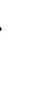
\includegraphics[max width=\textwidth, center]{2025_04_17_46e04c6acd873ea9558dg-142(11)}\\
a) 2\\
c) 4\\
d) 5\\
e) 6\\
f) 7\\
2

b) 3\\
b) 3\\
c) 4\\
10. Fie tablou unidimensional $\mathrm{v}=(5,8,1,3,6,7,4,9)$, elementele fiind numerotate de la 0 la 7. După executarea următoarelor instrucțiuni, tabloul unidimensional v va conține valorile:

\begin{verbatim}
Limbajul C++/C
i=0;
while(i<=3)
{
    if(v[i]<5)
        v[i]=2*v[i];
    if(v[7-i]>v[i])
\end{verbatim}

\begin{verbatim}
Limbajul Pascal
var a,b,c: integer;
begin
    a:=360; b:=0; c:=2;
    while a<>1 do
    begin
        if a mod c=0 then
        begin
            while a mod c=0 do
                a:=a div c;
            b:=b+1
        end;
        c:=c+1
    end;
    write(b)
end.
.
    var a,b,c: integer;
        *
*
    *
                            $
\end{verbatim}

$\qquad$\\

\includegraphics[max width=\textwidth, center]{2025_04_17_46e04c6acd873ea9558dg-142(2)}\\

\includegraphics[max width=\textwidth, center]{2025_04_17_46e04c6acd873ea9558dg-142(3)}\\

\includegraphics[max width=\textwidth, center]{2025_04_17_46e04c6acd873ea9558dg-142(5)}\\

\includegraphics[max width=\textwidth, center]{2025_04_17_46e04c6acd873ea9558dg-142(6)}\\

\includegraphics[max width=\textwidth, center]{2025_04_17_46e04c6acd873ea9558dg-142(1)}

\section*{a:}

\includegraphics[max width=\textwidth, center]{2025_04_17_46e04c6acd873ea9558dg-142}\\

\includegraphics[max width=\textwidth, center]{2025_04_17_46e04c6acd873ea9558dg-142(14)}

\begin{verbatim}
    *
            *
\end{verbatim}


\includegraphics[max width=\textwidth, center]{2025_04_17_46e04c6acd873ea9558dg-142(10)}\\

\includegraphics[max width=\textwidth, center]{2025_04_17_46e04c6acd873ea9558dg-142(7)}

\begin{verbatim}
        *
\end{verbatim}


\includegraphics[max width=\textwidth, center]{2025_04_17_46e04c6acd873ea9558dg-142(12)}\\

\includegraphics[max width=\textwidth, center]{2025_04_17_46e04c6acd873ea9558dg-142(4)}\\

\includegraphics[max width=\textwidth, center]{2025_04_17_46e04c6acd873ea9558dg-142(13)}\\

\includegraphics[max width=\textwidth, center]{2025_04_17_46e04c6acd873ea9558dg-142(8)}

\begin{verbatim}
*
\end{verbatim}

\begin{verbatim}
while i<=3 do
begin
if v[i]<5 then
    v[i]:=2*v[i];
if v[7-i]>v[i] then
\end{verbatim}

\begin{center}

\includegraphics[max width=\textwidth]{2025_04_17_46e04c6acd873ea9558dg-142(9)}
\end{center}

\begin{verbatim}
v[7-i]=v[7-i]-v[i];
i=i+1;
}
\end{verbatim}

a) $v=(5,8,2,6,6,4,4,3)$\\
c) $v=(5,8,2,6,6,5,4,4)$\\
e) $v=(5,8,8,6,6,4,4,4)$

\begin{verbatim}
v[7-i]:=v[7-i]-v[i];
i:=i+1
end;
\end{verbatim}

b) $v=(5,8,2,6,6,7,8,9)$\\
d) $v=(5,8,2,6,6,6,4,4)$\\
f) $v=(5,5,2,2,6,6,4,4)$\\
11. Variabilele s, i, c sunt de tip întreg. Variabila c memorează un număr natural par. În urma executării secvenței de instrucțiuni, variabila s are valoarea:

Limbajul C/C++\\
$\mathrm{s}=0$;\\
for (i=1;i<=c/2;i++)\\
s=s+i;\\
$\mathrm{s}=2$ * s ;\\
cout<<s; | printf("\%d", s); write(s);\\
Limbajul Pascal\\
s:=0; s:=s+i;\\
s: = ${ }^{*}$ * ;\\
for i:=1 to (c DIV 2) do\\
12. Variabilele i și c sunt de tip întreg, iar tablou unidimensional a are valorile ( $1,2,3,4,5,6,7$ ), primul element se află pe poziția 1 , al doilea element se află pe poziția 2 , ș.a.m.d. În urma executării instrucțiunilor, tabloul a va conține valorile:\\
a) $\frac{c \cdot(c+1)}{2}$\\
b) $c \cdot(c+1)$\\
c) $\frac{c \cdot(c+1)}{4}$\\
d) $\frac{c \cdot(c+2)}{4}$\\
e) $\frac{c \cdot(c-1)}{2}$\\
f) $\frac{c \cdot(c-1)}{4}$

Limbajul Pascal\\
for i:=1 to 7 do begin\\[0pt]
c:=a[i];\\[0pt]
a[i]:=a[7-i+1];\\[0pt]
a[7-i+1]:=c\\
end;

\begin{verbatim}
Limbajul C++/C
for(i=1;i<=7;i++)
{int c;
    c=a[i];
    a[i]=a[7-i+1];
    a[7-i+1]=c;
}
\end{verbatim}

a) $1 \begin{array}{llllll}2 & 3 & 4 & 6 & 7\end{array}$\\
b) $7 \quad 6 \quad 5 \quad 4 \quad 3 \quad 2 \quad 1$\\
c) 7654567\\
d) $\begin{array}{lllllll}1 & 2 & 3 & 4 & 3 & 2 & 1\end{array}$\\
e) 4321234\\
f) 4567654\\
13. În urma executării următorului program se va afișa:

\begin{verbatim}
Limbajul C++/C
int main()
{
    int c,i,nr=0;
    for(i=200; i<=300; i++)
        {
            c=i;
            while(c!=0)
                {
\end{verbatim}

\begin{verbatim}
Limbajul Pascal
var nr, i, c: integer;
begin
nr:=0;
for i:=200 to 300 do
    begin
        c:=i;
        while c<>0 do
            begin
\end{verbatim}

\begin{verbatim}
            if(c%2==1)
                nr++;
            c=c/10;
        }
    }
cout<<nr; | printf("%d", nr);
return 0;}
\end{verbatim}

\begin{verbatim}
    if c mod 2 = 1 then
        nr:=nr+1;
    c:=c div 10
    end
    end;
write(nr)
end.
\end{verbatim}

a) 50\\
b) 99\\
c) 100\\
d) 101\\
e) 102\\
f) 103\\
14. Subprogramul mat definit mai jos, cu doi parametri:

\begin{itemize}
  \item $n$, prin care primește un număr natural nenul ( $n \leq 100$ ),
  \item d, prin care primește elementele unui tablou bidimensional cu $\mathbf{n}$ linii și $\mathbf{n}$ coloane, numerotate de la 1 la n, determină:
\end{itemize}

\begin{verbatim}
Limbajul C++/C
int mat(int n, int d[][100])
{int e[100][100],i,j,k,p,matrice=0;
    if(n==1) {matrice=d[1][1];
                    return matrice;}
    else
    {
        for(i=1;i<=n;i++)
        {
            for(k=2;k<=n;k++)
                for(j=1;j<i;j++)
                    e[k-1][j]=d[k][j];
            for(k=2;k<=n;k++)
                for(j=i+1;j<=n;j++)
                    e[k-1][j-1]=d[k][j];
            if((i+1)%2==0) p=1;
            else p=-1;
    matrice=matrice+p*d[1][i]*mat(n-1,e);}
    return matrice;
    } }
\end{verbatim}

\begin{verbatim}
Limbajul Pascal
type matrix = array[1..100,1..100] of integer;
function mat(n:integer; d:matrix):integer;
var e: matrix;
            i,j,k,p,matrice: integer;
begin
matrice:=0;
if n=1 then
begin
    matrice:=d[1][1];
    mat:=matrice;
\end{verbatim}

\begin{verbatim}
end
else
begin
    for i:=1 to n do
        begin
        for k:=2 to n do
            for j:=1 to i-1 do
                e[k-1][j]:=d[k][j];
        for k:=2 to n do
            for j:=i+1 to n do
                e[k-1][j-1]:=d[k][j];
        if (i+j) MOD 2 =0 then
            p:=1
        else p:=-1;
        matrice:=matrice+p*d[1][i]*mat(n-1,e);
        end;
    mat:=matrice end end;
\end{verbatim}

a) pătratul matricei\\
b) transpusa matricei\\
c) determinantul matricei\\
d) matricea inversă\\
e) înmulțirea a două matrice\\
f) înmulțirea matricei cu o constantă\\
15. În urma executării subprogramului, pentru parametrii $\mathbf{v}, \mathbf{n}, \mathbf{k}, \mathrm{cu}$ valorile de intrare\\
$v=\left(\begin{array}{llll}0 & 1 & 2 & 3 \\ 4 & 5 & 6 & 7 \\ 8 & 9 & 0 & 1 \\ 2 & 3 & 4 & 5\end{array}\right), \mathrm{n}=4$ și $k=2 * \mathrm{n}$, se va afișa:

\begin{verbatim}
Limbajul C++/C
void afis(int v[][100],int n,int k)
{int i;
if(k!=1)
    {
        if(k%2==0) {
            for(i=1;i<=n;i++)
                if(k-i<=n && k-i>0)
                    cout<<v[i][k-i]; | printf("%d", v[i][k-i]);
}
        else {
            for(i=n;i>=1;i--)
                if(k-i<=n && k-i>0)
                    cout<<v[i][k-i]; | printf("%d", v[i][k-i]);
}
        afis(v,n,k-1);
    } }
\end{verbatim}

Limbajul Pascal\\
type matrice $=$ array of array of integer;

\begin{verbatim}
procedure afis(var v:matrice; n:integer; k:integer);
var i: integer;
begin
if k<>1 then
    begin
        if (k MOD 2)=0 then
            begin
            for i:=1 to n do
                if(k-i<=n) AND (k-i>0) then
                    write(v[i][k-i]);
            end
        else
            for i:=n downto 1 do
                if(k-i<=n) AND (k-i>0)
                    write(v[i][k-i])
    afis(v,n,k-1)
end end;
\begin{tabular}{ll} 
a) 5143073692852140 & b) 5417032963258410 \\
c) 0148523692307145 & d) 0412582963703415 \\
e) 0167093290672145 & f) 5498563245014398
\end{tabular}
\end{verbatim}

\section*{Varianta 26}
\begin{enumerate}
  \item Se dă o variabilă a care reține un număr natural nenul. Expresia care are valoarea $0 /$ false pentru orice număr natural nenul a este:\\
a) $\mathbf{C + + / C : ~}(a / 3+a / 7) \div 9$
\end{enumerate}

Pascal: (a DIV 3+a DIV 7) MOD 9\\
b) $\mathrm{C}++/ \mathrm{C}:(\mathrm{a} \% 10+\mathrm{a} \% 100 / 10) / 10$

Pascal: ((a MOD 10)+(a MOD 100) DIV 10) DIV 10\\
c) $\mathrm{C}++/ \mathrm{C}:((10-\mathrm{a} \% 10)+(10-\mathbf{a} \% 100 / 10)) / 10$

Pascal: ((10-(a MOD 10))+(10-(a MOD 100) DIV 10)) DIV 10\\
d) $\mathrm{C}++/ \mathrm{C}:(\mathrm{a} \% 5+\mathrm{a} \% 7) / 10$

Pascal: (a MOD 4+a MOD 6) DIV 10\\
e) C++/C: $(a \% 3+a \% 7) / 9$

Pascal: (a MOD 3+a MOD 7) DIV 9\\
f) $C++/ C:(a \% 10+a / 10) / 9$

Pascal: (a MOD 10+a DIV 10) DIV 9\\
2. Se dă un tablou unidimensional $\mathbf{v}=(\mathbf{3}, 5,8, \mathbf{4}, \mathbf{2}, \mathbf{6}, \mathbf{9}, 1)$ în care primul element se află pe poziția 0 și i o variabilă de tip întreg. În urma executării secvenței de instrucțiuni, elementele tabloului unidimensional $\mathbf{v}$ sunt:

\begin{verbatim}
Limbajul C++/C
i=0;
while(i<=6)
{
j=i+1;
v[i]=v[i]+v[j];
v[j]=v[i]-v[j];
v[i]=v[i]-v[j];
i=i+2;
}
\end{verbatim}

Limbajul Pascal i:=0; while i<=6 do begin j: =i+1; v[i]:=v[i]+v[j]; $v[j]:=v[i]-v[j] ;$ v[i]:=v[i]-v[j]; i:=i+2 end;\\
a) $v=(5,8,4,2,6,9,1,3)$\\
b) $v=(5,3,4,8,6,2,1,9)$\\
c) $v=(11,3,20,8,10,2,19,9)$\\
d) $v=(5,-7,4,0,6,10,1,6)$\\
e) $v=(3,1,9,6,2,4,8,5)$\\
f) $v=(9,1,2,6,8,4,3,5)$\\
3. Ș̦tiind că variabila i este de tip întreg și variabila a de tip șir de caractere reține cuvântul politehnica, în urma executării instrucțiunilor se va afișa:

\begin{verbatim}
Limbajul C++/C
for(i=0;i<=7;i++)
    if(a[i]<'n')
    a[i]='A'-'a'+a[i];
cout<<a; l printf("%s", a);
\end{verbatim}

\begin{verbatim}
Limbajul Pascal
for i:=1 to 8 do
    begin
        if a[i]<'n' then
            a[i]:=upcase(a[i])
\end{verbatim}

\begin{verbatim}
end;
write(a) ;
\end{verbatim}

a) poLItEHnICA\\
b) POliTehnica\\
c) POliTehnica\\
d) POliTehNICA\\
e) poliTEHNICA\\
f) polItEHnica\\
4.

Fie un tablou bidimensional $\mathbf{A}$, cu 4 linii și 4 coloane numerotate de la 0 la 3 care conține elemente de tip întreg și două variabile i și j de tip întreg. Valorile ce vor fi reținute în tabloul bidimensional A după executarea următoarelor instrucțiuni sunt:

\begin{verbatim}
Limbajul C++/C
i=3;
while(i>=0)
    {
        j=3;
        while(j>=0)
            {
                if((i+j)%2==0)
                    A[i][j]=i+j;
                else
                    if(i>j) A[i][j]=i;
                    else A[i][j]=j;
                j--;
            }
        i--;
    }
\end{verbatim}

\begin{verbatim}
Limbajul Pascal
i:=3;
while i>=0 do
    begin
    j:=3;
    while j>=0 do
        begin
        if (i+j) MOD 2 =0 then
            A[i,j]:=i+j
        else
            if i>j then
                A[i,j]:=i
            else
                A[i,j]:=j;
        j:=j-1
        end;
    i:=i-1
    end;
\end{verbatim}

a) $A=\left(\begin{array}{llll}0 & 0 & 2 & 0 \\ 0 & 2 & 1 & 4 \\ 2 & 1 & 4 & 2 \\ 0 & 4 & 2 & 6\end{array}\right)$\\
b) $A=\left(\begin{array}{llll}0 & 1 & 0 & 3 \\ 1 & 1 & 3 & 1 \\ 0 & 3 & 2 & 5 \\ 3 & 1 & 5 & 3\end{array}\right)$\\
c) $A=\left(\begin{array}{llll}0 & 1 & 2 & 3 \\ 1 & 1 & 3 & 3 \\ 2 & 3 & 2 & 5 \\ 3 & 3 & 5 & 3\end{array}\right)$\\
d) $A=\left(\begin{array}{llll}0 & 1 & 2 & 3 \\ 1 & 2 & 2 & 4 \\ 2 & 2 & 4 & 3 \\ 3 & 4 & 3 & 6\end{array}\right)$\\
е) $A=\left(\begin{array}{llll}0 & 2 & 1 & 3 \\ 2 & 1 & 3 & 3 \\ 1 & 3 & 2 & 5 \\ 3 & 3 & 5 & 3\end{array}\right)$\\
f) $A=\left(\begin{array}{llll}0 & 2 & 1 & 3 \\ 2 & 1 & 3 & 5 \\ 1 & 3 & 5 & 3 \\ 3 & 5 & 3 & 3\end{array}\right)$\\
5.

Fie o stivă inițial vidă. Cu ajutorul subprogramelor Ad(x), respectiv El() este adăugat elementul $\mathbf{x}$, respectiv șters un element din stivă. Suma elementelor din stivă după executarea operațiilor următoare este:\\
Ad (3) Ad (7) Ad (5) El() El() Ad (8)\\
a) 3\\
b) 7\\
c) 10\\
d) 11\\
e) 12\\
f) 13\\
6. Se dă mulțimea $A=\{\mathbf{1}, \mathbf{4}, 5,8,9\}$. Un algoritm generează în ordine crescătoare, toate numerele naturale de $\mathbf{n}$ cifre, folosind cifre distincte din mulțimea $\mathbf{A}$, care nu au alăturate cifre de aceeași paritate. Dacă pentru $\mathrm{n}=4$, primele patru soluții generate sunt: 1458, $1498,1854,1894$, numărul de soluții pe care le va genera algoritmul este:\\
a) 12\\
b) 16\\
c) 20\\
d) 24\\
e) 28\\
f) 30\\
7. Șirul care poate reprezenta valorile gradelor nodurilor unui graf neorientat cu 6 noduri este:\\
a) 250212\\
b) 221112\\
c) 227221\\
d) 220042\\
e) 231122\\
f) 222112\\
8. Șirul de valori care poate fi vectorul de tați al unui arbore cu 8 noduri este:\\
a) $T=(01832554)$\\
b) $T=(03724583)$\\
c) $T=(01124587)$\\
d) $T=(05731312)$\\
e) $T=(01024633)$\\
f) $T=(85731312)$\\
9. Știind că $\mathbf{i}, \mathbf{j}, \mathbf{s}$ și a sunt patru variabile de tip întreg, pentru orice valoare naturală nenulă a variabilei a, după executarea instrucțiunilor, valoarea afișată corespunde formulei matematice:

\begin{verbatim}
Limbajul C++/C
s=0;
for(i=1;i<=a;i++)
    {
        j=1;
        while(j<=i)
            {
                s++;
                j++;
            }
        j=i+1;
        do
            {
                s++;
                j++;
            }while(j<=a);
    }
cout<<s--; | printf("%d", s--);
\end{verbatim}

\begin{verbatim}
Limbajul Pascal
s:=0;
for i:=1 to a do
begin
    j:=1;
    while j<=i do
    begin
        s:=s+1;
        j:=j+1
    end;
    j:=i+1;
    repeat
        s:=s+1;
        j:=j+1;
    until j>a;
end;
write(s);
\end{verbatim}

a) $a(a+1)$\\
b) $a^{2}+1$\\
c) $a^{2}$\\
d) $a^{2}-1$\\
e) $a(a-1)$\\
f) $2 a^{2}-1$\\
10. Subprogramul afis primește ca parametru un tablou bidimensional v cu n linii și n coloane, numerotate de la 1 la n, unde

$$
v=\left(\begin{array}{llll}
0 & 1 & 2 & 3 \\
4 & 5 & 6 & 7 \\
8 & 9 & 0 & 1 \\
2 & 3 & 4 & 5
\end{array}\right), \mathrm{n}=4 \text { și } \mathrm{k}=2 \cdot \mathrm{n} .
$$

Pentru valorile date, afis ( $\mathbf{v}, \mathbf{n}, \mathbf{k}$ ) va afișa:

\begin{verbatim}
Limbajul C++/C
void afis(int v[100][100],int n,int k)
{int i;
if(k>1)
    { for(i=n;i>=1;i--)
        if(k-i<=n && k-i>0)
            cout<<v[i][k-i]; | printf("%d", v[i][k-i]);
afis(v,n,k-2);}
}
\end{verbatim}

Limbajul Pascal\\
type matrice $=$ array [1..100,1..100] of integer;\\
procedure afis (var v:matrice; n:integer; k:integer);\\
var i: integer;\\
begin\\
if $k<>1$ then\\
begin\\
for i:=n downto 1 do\\
if(k-i<=n) AND (k-i>0) then\\[0pt]
write (v[i,k-i]);\\
afis(v,n,k-2)\\
end\\
end;\\
a) 08523075\\
b) 57032580\\
c) 02587035\\
d) 53078520\\
e) 35087250\\
f) 70358520\\
11. Știind că subprogramul functie corespunde funcției matematice $f(x)=3 \cdot \mathbf{x - 1}$, pentru orice $\mathbf{x}$ număr întreg, $a b c(t, c)$ va calcula:

\begin{verbatim}
Limbajul C++/C
int functie(int x)
{return 3*x-1;}
int abc(int t, int c)
{ if(c==0) return t;
    else
        return abc(functie(t),c-1);}
\end{verbatim}



\begin{verbatim}
function functie(var x:integer):integer;
begin
    functie:=3*x-1
end;
function abc(t,c:integer):integer;
begin
    if c=0 then
            abc:=t
    else
        abc:=abc(functie(t),c-1)
end;
\end{verbatim}

a) $\underbrace{\boldsymbol{f}(\boldsymbol{t}) \circ \ldots \circ \boldsymbol{f}(\boldsymbol{t})}_{c-1}$\\
b) $\underbrace{f(t)+\cdots+f(t)}_{c-1}$\\
c) $f(t)^{c}$\\
d) $\boldsymbol{c} * \boldsymbol{f}(\boldsymbol{t})$\\
e) $(\boldsymbol{c}-1) * \boldsymbol{f}(\boldsymbol{t})$\\
f) $\underbrace{f(t) \circ \ldots \circ f(t)}_{c}$\\
12. După executarea următoarelor instrucțiuni se va afișa:

\begin{verbatim}
Limbajul C++/C
char a[20][20];
int i;
strcpy(a[1],"bacalaureat");
strcpy(a[2],"liceu");
strcpy(a[3],"examene");
strcpy(a[4],"politehnica");
for(i=1;i<=4;i++)
        cout<<a[i][2*i];
| printf("%d", a[i][2*i]);
\end{verbatim}

\begin{verbatim}
Limbajul Pascal
var a:array[1..20] of
string;
    i:integer;
begin
a[1]:='bacalaureat';
a[2]:='liceu';
a[3]:='examene';
a[4]:='politehnica';
for i:=1 to 4 do
    write(a[i,2*i+1])
end.
\end{verbatim}

a) aenn\\
b) teen\\
c) cunc\\
d) cuei\\
e) bceh\\
f) ceen\\
13. Următoarele instrucțiuni vor afișa:

\begin{verbatim}
Limbajul C++
int f1(int x, int &y)
{
    x=x+2;
    y=y-1;
    return x+y;
    x=x+1;
}
\end{verbatim}

\begin{verbatim}
Limbajul C
int f1(int x, int *y)
{
    x=x+2;
    *y=*y-1;
    return x+*y;
    x=x+1;
}
\end{verbatim}

\begin{verbatim}
    int main()
    {
    int n=3,m=6;
    cout<<<f1 (f1 (m,n) ,m);
    cout<<" "<<m;
    }
\end{verbatim}

\begin{verbatim}
int main()
{
int n=3,m=6;
printf("%d ",
f1(f1 (m,&n) ,&m)) ;
printf("%d", m);
}
\end{verbatim}

Limbajul Pascal\\
function $f 1(x: i n t e g e r ; ~ v a r ~ y: i n t e g e r) ~: i n t e g e r ; ~$\\
begin\\
$\mathrm{x}:=\mathrm{x}+2$;\\
$y:=y-1$;\\
f1: =x+y;\\
$\mathrm{x}:=\mathrm{x}+1$\\
end;\\
var m,n: integer;\\
begin\\
m: =6;\\
n: =3;\\
write (f1 (f1 (m, n) , m),' ', m)\\
end.\\
a) 175\\
b) $17 \quad 6$\\
c) $10 \quad 5$\\
d) $10 \quad 6$\\
e) 116\\
f) $10 \quad 7$\\
14. Valorile care vor fi memorate în tabloul bidimensional $\mathbf{b}$, cu liniile și coloanele numerotate de la 1 la $n$, după apelul matrice ( $\mathbf{a}, \mathbf{b}, \mathrm{n}, \mathrm{q}$ ), unde

\begin{verbatim}
a=( (\begin{array}{lll}{2}&{3}&{4}\\{3}&{4}&{5}\\{4}&{5}&{6}\end{array}),\quadb=\mp@subsup{O}{3}{},\quad\textrm{n}=3,\quad\textrm{q}=2,\mathrm{ sunt:}
Limbajul C++/C
void matrice(int a[][100], int b[][100], int n, int q)
{int i,j,k;
    if(q>1)
        {
            for(i=1;i<=n;i++)
                for(j=1;j<=n;j++)
                    for(k=1;k<=n;k++)
                        b[i][j]=b[i][j]+a[i][k]*a[k][j];
            matrice(a,b,n,q-1);
        }
}
Limbajul Pascal
type matrix = array [1..100,1..100] of integer;
procedure matrice(a:matrix; b:matrix; n:integer;
q:integer);
var i,j,k: integer;
\end{verbatim}

\begin{verbatim}
begin
    if q>1 then
    begin
    for i:=1 to n do
        for j:=1 to n do
            for k:=1 to n do
                b[i,j]:=b[i,j]+a[i,k]*a[k,j];
        matrice(a,b,n,q-1)
    end
end;
a) $b=\left(\begin{array}{lll}2 & 3 & 4 \\ 3 & 4 & 5 \\ 4 & 5 & 6\end{array}\right)$
b) $\boldsymbol{b}=\left(\begin{array}{lll}47 & 38 & 29 \\ 62 & 50 & 38 \\ 77 & 62 & 47\end{array}\right)$
c) $b=\left(\begin{array}{ccc}4 & 6 & 8 \\ 6 & 8 & 10 \\ 8 & 10 & 12\end{array}\right)$
d) $\boldsymbol{b}=\left(\begin{array}{ccc}4 & 9 & 16 \\ 9 & 16 & 25 \\ 16 & 25 & 36\end{array}\right)$
е) $\boldsymbol{b}=\left(\begin{array}{lll}\mathbf{2 9} & \mathbf{3 8} & \mathbf{4 7} \\ \mathbf{3 8} & \mathbf{5 0} & \mathbf{6 2} \\ \mathbf{4 7} & \mathbf{6 2} & \mathbf{7 7}\end{array}\right)$
f) $b=\left(\begin{array}{lll}77 & 62 & 47 \\ 62 & 50 & 38 \\ 47 & 38 & 29\end{array}\right)$
\end{verbatim}

\begin{enumerate}
  \setcounter{enumi}{14}
  \item În urma executării programului de mai jos se afișează:
\end{enumerate}

\begin{verbatim}
Limbajul C++
#include <iostream>
using namespace std;
void functie(int &a,int &b)
{ b=3*b;
        a=2*a;}
int main()
{ int n=4;
        functie(n,n);
        cout<<n;}
\end{verbatim}

\begin{verbatim}
Limbajul C
#include <stdio.h>
void functie(int *a,int *b)
{ *b=3*(*b);
        *a=2*(*a);}
int main()
{ int n=4;
        functie(&n,&n);
        printf("%d", n);
}
\end{verbatim}

\begin{verbatim}
Limbajul Pascal
procedure functie (var a:integer; var b:integer);
begin
        b:=3*b;
        a:=2*a
end;
var n:integer;
begin
            n:=4;
            functie(n,n);
            write(n)
end.
\end{verbatim}

a) eroare\\
b) 4\\
c) 6\\
d) 12\\
e) 14\\
f) 24

\section*{Varianta 27}
\begin{enumerate}
  \item Rezultatul expresiei de mai jos este:
\end{enumerate}

Limbajul C++/C\\
$16 /(-5 \% 3)$ * 3\\
a) 48\\
b) -24\\
c) $\mathbf{- 4 8}$\\
d) -2\\
e) 2\\
f) 6

Limbajul Pascal\\
16 div $(-5 \bmod 3)$ * 3\\
2. Expresia corespunzătoare penultimei cifre a numărului natural având cel puțin două cifre reținut de variabila întreagă $n$ este:\\
Limbajul C++/C\\
a) $n / 10 / 10$\\
b) $\mathrm{n} / 10 \% 10$\\
c) $n \% 10 \% 10$\\
d) $n \% 10 / 10$\\
e) $n \% 10 / 100$\\
f) $n / 100 \% 10$

Limbajul Pascal\\
a) n div $10 \operatorname{div} 10$\\
b) n div $10 \bmod 10$\\
c) $\mathrm{n} \bmod 10 \bmod 10$\\
d) $n \bmod 10 \operatorname{div} 10$\\
e) $n \bmod 10 \operatorname{div} 100$\\
f) $\mathrm{n} \operatorname{div} 100 \bmod 10$\\
3. Afirmația adevărată în privința secvenței de instrucțiuni de mai jos este:

\begin{verbatim}
Limbajul C++/C
d = 1;
while (d * d <= n)
{
    if (n % d == 0)
    {
        d1 = d;
        d2 = n / d;
    }
    d++;
}
\end{verbatim}

\begin{verbatim}
Limbajul Pascal
d := 1;
while d * d <= n do
    begin
        if n mod d = 0 then
            begin
                d1 := d;
                d2 := n div d
            end;
        d := d + 1
    end
\end{verbatim}

a) La final d1 și d2 vor fi egale doar dacă n reține un număr prim.\\
b) La final d1 și d2 vor fi egale doar dacă n reține cubul unui număr prim.\\
c) La final d1 și d2 vor fi egale doar dacă n reține un număr impar.\\
d) La final d1 ș̦i d2 vor fi egale doar dacă n reține un număr par.\\
e) La final d1 și d2 vor fi egale doar dacă $\mathbf{n}$ reține 0 .\\
f) La final d1 și d2 vor fi egale doar dacă $\mathbf{n}$ reține un număr pătrat perfect.\\
4. Secvența de instrucțiuni de mai jos ordonează crescător cele n elemente ale tabloului unidimensional $\mathbf{v}$, în care primul element este memorat pe poziția 0 , dacă punctele de suspensie sunt înlocuite cu:

\begin{verbatim}
Limbajul C++/C
for (i = 0; i < n - 1; i++)
{
    ...
    {
        if (v[j] > v[j+1])
\end{verbatim}

\begin{verbatim}
Limbajul Pascal
for i := 0 to n - 2 do
    begin
        ...
            begin
                if v[j] > v[j+1] then
\end{verbatim}

a) for (j $=n-2$; $j>=i ; j--)$\\
b) for (j $=0$; $\mathbf{j}<=\mathbf{i} ; ~ j++$ )\\
c) for ( $\mathbf{j}=\mathrm{n}-\mathrm{i} ; \mathrm{j}>=\mathrm{i} ; \mathrm{j}-\mathrm{-})$\\
d) for ( $j=1 ; j<i ; j++$ )\\
e) for ( $j=n-1$; $j>i ; j--)$\\
a) for ( $j=n-2 ; j>=i ; j--)$

\begin{center}
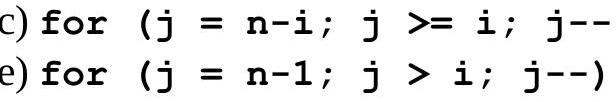
\includegraphics[max width=\textwidth]{2025_04_17_46e04c6acd873ea9558dg-155(2)}
\end{center}

\begin{verbatim}
f) for ( $\mathbf{j}=1 ; j<=i+1 ; j++$ )
\end{verbatim}

Limbajul Pascal\\
a) for $j:=n-2$ downto $i$ do\\
b) for $j:=0$ to $i$ do\\
c) for $j:=n-i$ downto $i$ do\\
d) for $j:=1$ to $i-1$ do\\
e) for $j:=n-1$ downto $i+1$ do\\
f) for $j:=1$ to $i+1$ do\\
f) for $j:=1$ to $i+1$ do\\
for $j:=0$ to $i$ do\\
for $j:=1$ to $i-1$ do\\
5. Subprogramul $\mathbf{f}$ este definit mai jos. O condiție necesară și suficientă pentru ca numărul natural mai mare strict ca 1 reținut de variabila n să fie prim este:

\begin{verbatim}
Limbajul C++/C
        int f(int d, int n)
{
                do
    {
                        d++;
    }
    while (n % d != 0);
    return d;
}
            {
                {
                    while (n
        }
\end{verbatim}

Limbajul C/C++\\
a) $f(2, n)=n$\\
b) $f(2, n)==2$\\
c) $f(1, n)=n$\\
d) $f(1, n)==1$\\
e) $f(1, n-1)==n$\\
f) $f(2, n-1)=2$

Limbajul Pascal\\
a) $f(2, n)=n$\\
b) $f(2, n)=2$\\
c) $f(1, n)=n$\\
d) $f(1, n)=1$\\
e) $f(1, n-1)=n$\\
f) $f(2, n-1)=2$

\begin{verbatim}
Limbajul Pascal
function $f(d, n$ : integer) :
integer;
begin
repeat
        d := d + 1;
    until n mod d = 0;
    f := d
    end;
                        Limbajul Pascal
                        function f(d, n: integer):
\end{verbatim}

\begin{center}

\includegraphics[max width=\textwidth]{2025_04_17_46e04c6acd873ea9558dg-155(1)}
\end{center}

\begin{verbatim}
end
end
\end{verbatim}

\begin{center}

\includegraphics[max width=\textwidth]{2025_04_17_46e04c6acd873ea9558dg-155}
\end{center}

\begin{verbatim}
    en
\end{verbatim}

\begin{verbatim}
end
j+1];
v[j] v[j+1] := aux
        begin
    aux := v[j];
                aux
\end{verbatim}

\begin{verbatim}
*
\end{verbatim}

\begin{verbatim}
                    ]
\end{verbatim}

\begin{verbatim}
*
\end{verbatim}

\begin{verbatim}
        {
            aux = v[j];
            v[j] = v[j+1];
            v[j+1] = aux;
        }
    }
}
                        v[j]= v[j+1]
    }
*
\end{verbatim}

\begin{verbatim}
Limbajul C++/C
\end{verbatim}

\begin{verbatim}
            正
        Limbajul Pascal
\end{verbatim}

\begin{enumerate}
  \setcounter{enumi}{5}
  \item Numărul de muchii care trebuie adăugate unui arbore cu 10 vârfuri astfel încât acesta să devină graf complet este:\\
a) 9\\
b) 10\\
c) 11\\
d) 35\\
e) 36\\
f) 37
  \item Suma elementelor aflate pe diagonala principală a matricei a, cu 5 linii și 5 coloane numerotate de la 0 la 4, ale cărei elemente sunt actualizate în secvența de instrucțiuni de mai jos este:
\end{enumerate}

\begin{verbatim}
Limbajul C++/C
n = 5;
for (i = 0; i < n; i++)
\end{verbatim}

\begin{verbatim}
Limbajul Pascal
n := 5;
for i := 0 to n - 1 do
\end{verbatim}

\begin{verbatim}
{
    for (j = 0; j < n; j++)
    {
        a[i][j] = (n - i) * n - j;
    }
}
\end{verbatim}

\begin{verbatim}
begin
    for j := 0 to n - 1 do
        begin
            a[i,j] := (n-i)*n - j
        end
end
\end{verbatim}

a) 15\\
b) 20\\
c) 35\\
d) 55\\
e) 65\\
f) 70\\
8. O variantă care poate corespunde șirului gradelor interne ale vârfurilor grafului orientat alăturat este:\\
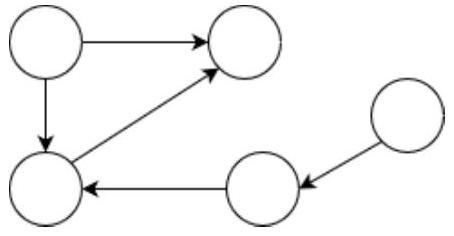
\includegraphics[max width=\textwidth, center]{2025_04_17_46e04c6acd873ea9558dg-156(1)}\\
a) $(2,1,1,1,0)$\\
b) $(1,1,1,1,0)$\\
c) $(2,1,0,2,0)$\\
d) $(2,0,2,2,0)$\\
e) $(2,0,0,3,0)$\\
f) $(2,0,1,1,0)$\\
9. Un algoritm Backtracking generează ultimele două soluții pilo și poli, având ca date de intrare cuvântul poli. O variantă care poate reprezenta descrierea algoritmului este:\\
a) Algoritmul generează în ordine invers lexicografică anagramele cuvântului citit.\\
b) Algoritmul generează în ordine lexicografică anagramele cuvântului citit.\\
c) Algoritmul generează în ordine lexicografică anagramele cuvântului citit care nu au vocale pe poziții alăturate.\\
d) Algoritmul generează în ordine lexicografică anagramele cuvântului citit care nu au consoane pe poziții alăturate.\\
e) Algoritmul generează în ordine lexicografică anagramele cuvântului citit care nu au vocale pe ultima poziție.\\
f) Algoritmul generează în ordine invers lexicografică anagramele cuvântului citit care nu au consoane pe ultima poziție.\\
10. Programul de mai jos afișează pe ecran textul Poli 2020 dacă punctele de suspensie sunt înlocuite cu:

\begin{verbatim}
Limbajul C++/C
#include <stdio.h>
#include <string.h>
int main()
{
    char s[256], t[256];
    strcpy(s,"Politehnica 2020");
    ...
    strcpy(s + 4, t);
    puts(s);
    return 0;
}
Limbajul C++/C
\end{verbatim}

\begin{verbatim}
Limbajul Pascal
var s, t: string;
begin
    s:='Politehnica 2020';
    ...
    s:=copy(s, 1, 4) + t;
    writeln(s)
end.
\end{verbatim}

\begin{center}

\includegraphics[max width=\textwidth]{2025_04_17_46e04c6acd873ea9558dg-156}
\end{center}

\begin{verbatim}
d) strcpy(t, strchr (s, " "));
\end{verbatim}

a) strcpy (t, strchr (s, ' '));\\
b) strcpy (t, strcpy (s, ' '));\\
c) strcat(t, strchr (s, '2'));\\
e) strcat(t, strcpy (s, "2"));\\
f) strcpy (t, strchr(s, "2"));

Limbajul Pascal\\
a) $t:=\operatorname{copy}(s, \operatorname{pos}(' \quad ', s), 5)$;\\
b) $\mathrm{t}:=\operatorname{copy}(\mathrm{s}, \operatorname{copy}(1 \mathrm{~s}, \mathrm{~s}), 4)$;\\
c) $t:=s+\operatorname{pos}\left({ }^{\prime} 2 ', s\right) ;$\\
d) $t:=\operatorname{copy}(s, \operatorname{pos}(" \mathrm{"}, \mathrm{s}), 5)$;\\
e) $t:=\operatorname{copy}(s$, copy ("2", s), 4);\\
f) $t:=$ copy (s, pos ("2", s), 5);\\
11. Subprogramul $f$ este definit mai jos. Valoarea returnată la apelul $f(24,34)$ este:

\begin{verbatim}
Limbajul C++/C
int f(int a, int b)
{
    int r;
    if (a >= b)
    {
        r = a;
    }
    else if (a % 10 == b % 10)
    {
        r = 2 + f(a + 1,b);
    }
    else if (a % 3 == b % 3)
    {
        r=1 + f(a + 1,b - 1);
    }
    else
    {
        r = f(a, b - 2);
    }
    return r;
}
\end{verbatim}

\begin{verbatim}
Limbajul Pascal
function f(a, b: integer):
integer;
var r: integer;
begin
    if a >= b then
        begin
            r := a;
        end
    else
    if a mod 10 = b mod 10 then
        begin
            r := 2 + f(a + 1,b)
        end
    else if a mod 3 = b mod 3
then
        begin
            r := 1 + f(a + 1, b - 1)
        end
    else
        begin
            r := f(a, b - 2)
        end;
    f := r
end;
\end{verbatim}

a) 30\\
b) 31\\
c) 32\\
d) 33\\
e) 34\\
f) 35\\
12. Numărul maxim de muchii care pot fi eliminate din graful neorientat alăturat astfel încât acesta să conțină cel puțin trei cicluri elementare distincte este:\\
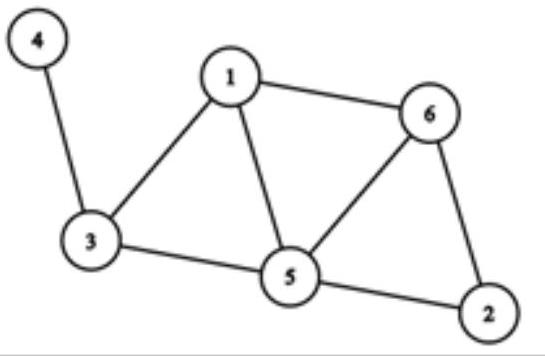
\includegraphics[max width=\textwidth, center]{2025_04_17_46e04c6acd873ea9558dg-157}\\
a) 1\\
b) 6\\
c) 2\\
d) 4\\
e) 5\\
f) 3\\
13. Se generează în ordine lexicografică vectorii de tați corespunzători tuturor arborilor cu rădăcină având exact 6 noduri. Prin înălțimea unui arbore cu rădăcină înțelegem numărul de muchii ale celui mai lung lanț elementar care unește rădăcina cu un alt nod. A doua soluție corespunzătoare unui arbore cu înălțimea 3 este:\\
a) 012311\\
b) 011125\\
c) 011126\\
d) 011135\\
e) 011112\\
f) 011145\\
14. Subprogramul rad de mai jos calculează și returnează cel mai mic număr care ridicat la pătrat este mai mare sau egal cu numărul natural reținut de $\mathbf{x}$ (partea întreagă superioară a lui radical din $\mathbf{x}$ ) dacă punctele de suspensie sunt înlocuite cu:

\begin{verbatim}
Limbajul C++/C
int rad(int s, int d, int x)
{
    int rez, m;
    if (s == d)
    {
        rez = s;
    }
    else
    {
        m = (s + d) / 2;
        if (...)
        {
            rez = rad(s, m, x);
        }
        else
        {
            rez = rad(m + 1, d, x);
        }
    }
    return rez;
}
\end{verbatim}

\begin{verbatim}
Limbajul Pascal
function rad(s,d,x: integer)
        :integer;
var m, rez: integer;
begin
    if s = d then
        begin
            rez := s
        end
    else
        begin
            m := (s + d) div 2;
            if ... then
                begin
                    rez := rad(s, m, x)
                end
            else
                begin
                    rez := rad(m+1,d, x)
                end
        end;
    rad := rez
end;
\end{verbatim}

Limbajul C++/C\\
a) $m * m==x$\\
b) $m * m>=x$\\
c) $m * m<=x$\\
d) $m * m>x$\\
e) $m$ * $m<x$\\
f) $m$ * $m \quad!=x$

Limbajul Pascal\\
a) $m * m=x$\\
b) $m * m>=x$\\
c) $m * m<=x$\\
d) $m * m>x$\\
e) $m * m<x$\\
f) $m * m<x$\\
15. Fie un tablou unidimensional $\mathbf{v}$ care reține n numere naturale: $\mathrm{v}[\mathrm{0}], \mathrm{v}[1], \ldots, \mathrm{v}[\mathrm{n}-$ 1] și un număr întreg $t$. Secvența de instrucțiuni de mai jos are ca efect obținerea lungimii maxime $\operatorname{lmax}$ a unei subsecvențe $\mathrm{v}[\mathrm{k}], \mathrm{v}[\mathrm{k}+1]$, ... $\mathrm{v}[\mathrm{k}+1 \max -1]$ având suma elementelor mai mică sau egală cu $t$ dacă punctele de suspensie sunt înlocuite cu:

Limbajul C++/C

\begin{verbatim}
s = 0;
j = 0;
lmax = 0;
\end{verbatim}

Limbajul Pascal

\begin{verbatim}
s := 0;
j := 0;
lmax := 0;
\end{verbatim}

\begin{verbatim}
for (i = 0; i < n; i++)
{
    s += v[i];
    while (j <= i && s > t)
    {
        j++;
    }
    if (i - j + 1 > lmax)
    {
        lmax = i - j + 1;
    }
}
\end{verbatim}

Limbajul C++/C\\
a) $\mathbf{s}+=\mathbf{v}[j]$;\\
b) i-- ;\\
c) $\mathbf{s}-=\mathbf{v}[\mathbf{i}]$;\\
d) $s \quad-=v[j]$;\\
e) $\mathbf{s}+=\mathbf{v}[i]$;\\
f) $i++$;\\
Limbajul Pascal\\
a) $s:=s+v[j]$;\\
b) i $:=i-1$;\\
c) $s:=s-v[i]$;\\
d) $s:=s-v[j]$;\\
e) $s:=s+v[i]$;\\
f) $i:=i+1$;

\section*{Varianta 28}
\begin{enumerate}
  \item Expresia corespunzătoare mediei aritmetice a patru numere reale memorate în variabilele a,b, cşi d este:\\
a) $a+b+c+d / 4$\\
b) $(a+b+c+d) * 1 / 2$\\
c) $(a+b+c+d) * 0.4$\\
d) $(a+b+c+d) * 0.25$\\
e) $(a+b+c+d) * 4.0$\\
f) $(a+b+c+d) * 1.4$
  \item În secvențele de instrucțiuni $\mathbf{S} 1$ și $\mathbf{S} 2$ variabilele $\mathbf{n}$ și $\mathbf{p}$ sunt de tip întreg. Obținerea în variabila $\mathbf{p}$ a primei cifre a numărului reținut inițial de $\mathbf{n}$ este realizată:
\end{enumerate}

\begin{verbatim}
Limbajul C/C++
//S1
p = n;
while (p > 9)
{
        p /= 10;
}
Limbajul Pascal
\end{verbatim}

\begin{verbatim}
{S1}
p := n;
while p > 9 do
        begin
            p := p div 10
        end
\end{verbatim}

a) doar de $\mathbf{S 1}$

\begin{verbatim}
//S2
do
{
    p = n % 10;
    n /= 10;
}
while (n != 0);
{S2 }
repeat
    p := n mod 10;
    n := n div 10
until n = 0;
\end{verbatim}

c) atât de $\mathbf{S} 1$, cât și de $\mathbf{S} 2$\\
b) doar de $\mathbf{S 2}$\\
e) doar de $\mathbf{S 1}$, dacă n are o singură\\
d) doar folosind o cu totul altă secvență\\
f) doar de S2, dacă $\mathbf{n}$ are mai multe cifre\\
3. În urma executării secvenței de instrucțiuni de mai jos variabila $n \boldsymbol{n}$ va reține numărul divizorilor primi ai numărului natural nenul reținut inițial de variabila $\mathbf{n}$ dacă punctele de suspensie sunt înlocuite cu:

\begin{verbatim}
Limbajul C++/C
d = 2;
nr = 0;
while (n > 1)
{
        p = 0;
        while (...)
        {
            p = 1;
            n /= d;
        }
    nr += p;
    d++;
}
\end{verbatim}

Limbajul Pascal

\begin{verbatim}
d := 2;
nr := 0;
while n > 1 do
    begin
        p := 0;
        while ... do
            begin
                p := 1;
                n := n div d
            end;
        nr := nr + p;
        d := d + 1
    end
\end{verbatim}

Limbajul C++/C\\
a) $d * d<n$\\
b) $n<d$\\
c) $\mathrm{n}>\mathrm{d}$\\
d) $d+d<n$\\
e) $n \% d!=0$\\
f) $n \% d==0$

Limbajul Pascal\\
a) $d \star d<n$\\
b) $n<d$\\
c) $\mathrm{n}>\mathrm{d}$\\
d) $d+d<n$\\
e) $n \bmod d<>0$\\
f) $n \bmod d=0$\\
4. Vectorul vare $\mathbf{n}$ componente întregi, numerotate de la $\mathbf{0}$, ordonate crescător. Pentru ca în urma executării secvenței de instrucțiuni de mai jos să se insereze valoarea întreagă reținută de $\mathbf{x}$ în vectorul $\mathbf{v}$ și acesta să rămână ordonat, punctele de suspensie trebuie înlocuite cu:\\
Limbajul C++/C\\
i = n - 1;\\[0pt]
while (i >= 0 \&\& v[i] > x)\\
$\{$

\begin{verbatim}
v[i+1] = v[i];
i--;
}
...;
\end{verbatim}

\begin{verbatim}
Limbajul Pascal
i := n - 1;
while (i>=O) and (v[i]>x) do
    begin
        v[i+1] := v[i];
        i := i - 1;
    end;
...;
\end{verbatim}

n++;\\
Limbajul C++/C\\
a) $\mathbf{x}=v[i+1]$\\
b) $v[i]=x$\\
c) $v[n]=x$\\
d) $v[i-1]=x$\\
e) $v[i+1]=x$\\
f) $v[n+1]=x$

Limbajul Pascal\\
a) $\mathbf{x}:=v[i+1]$\\
b) $\mathrm{v}[\mathrm{i}]:=\mathrm{x}$\\
c) $v[n]:=x$\\
d) $v[i-1]:=x$\\
e) $\mathrm{v}[\mathrm{i}+1]:=\mathrm{x}$\\
f) $v[n+1]:=x$\\
5. În urma executării secvenței de instrucțiuni de mai jos suma elementelor pare ale matricei a, cu 5 linii și 5 coloane numerotate de la 0 la 4 va fi:

\begin{verbatim}
Limbajul C/C++
n = 5;
for (i = 0; i < n; i++)
{
    for (j = 0; j < n; j++)
    {
        a[i][j] = i - j + n;
    }
}
\end{verbatim}

a) 20\\
b) 60\\
c) 62\\
d) 64\\
e) 61\\
f) 12

\begin{verbatim}
Limbajul Pascal
n := 5;
for i := 0 to n - 1 do
    begin
        for j := 0 to n - 1 do
            begin
                a[i,j] := i - j + n
            end;
    end;
\end{verbatim}

\begin{enumerate}
  \setcounter{enumi}{5}
  \item Subprogramul $\mathbf{f}$ este definit mai jos. Apelul care returnează valoarea 0 este:
\end{enumerate}

\begin{verbatim}
Limbajul C++/C
int f(int n)
{
    int r = 0;
    while (r * r < n)
    {
        r++;
\end{verbatim}

\begin{verbatim}
Limbajul Pascal
function f(n:integer):integer;
var r: integer;
begin
    r := 0;
    while r * r < n do
        begin
\end{verbatim}

\begin{verbatim}
    }
    return r * r - n;
}
\end{verbatim}

a) $f(23)$\\
b) $f(225)$\\
c) $\mathrm{f}(17)$\\
d) $\pounds(131)$\\
e) $\pounds(122)$\\
f) $\mathrm{f}(1000)$

\begin{verbatim}
        r := r + 1
        end;
    f := r*r - n
end;
\end{verbatim}

\begin{enumerate}
  \setcounter{enumi}{6}
  \item Un graf orientat tare conex are șirul gradelor externe ale vârfurilor sale ( $3,1,1,1$ ). Graful nu are arce cu extremitățile identice (bucle). O variantă care poate reprezenta șirul gradelor interne ale vârfurilor grafului este:\\
a) $(6,0,0,0)$\\
b) $(2,1,3,2)$\\
c) $(2,2,2,0)$\\
d) $(1,1,2,2)$\\
e) $(1,1,1,2)$\\
f) $(0,0,1,5)$
  \item Numărul nodurilor terminale (frunze) ale arborelui cu rădăcină corespunzător vectorului de tați ( $7,4,0,3,7,3,3,4$ ) este:\\
a) 3\\
b) 7\\
c) 5\\
d) 0\\
e) 8\\
f) 4
  \item Programul de mai jos afișează numărul aparițiilor caracterului $\mathbf{c}$ în cuvântul $\mathbf{s}$ dacă punctele de suspensie sunt înlocuite cu:
\end{enumerate}

\begin{verbatim}
Limbajul C++/C
#include <stdio.h>
#include <string.h>
int main()
{
    char s[256], c, *p;
    int nr;
    scanf("%s %c", s, &c);
    p = strchr (s, c);
    nr = 0;
    while (p != NULL)
    {
        nr++;
        ...;
        p = strchr (s, c);
    }
    printf("%d", nr);
    return 0;
}
Limbajul C/C++
\end{verbatim}

a) strcpy ( $p, p+1$ )\\
b) strcpy $(p+1, p)$\\
c) $\operatorname{strcat}(\mathrm{s}, \mathrm{p}+1)$\\
d) $\mathrm{p}++$\\
e) $\operatorname{strcat}(s, p)$\\
f) $\mathrm{p}--$

Limbajul Pascal\\
a) delete ( $\mathrm{s}, \mathrm{p}, 1$ )\\
b) delete ( $p, s, 1$ )\\
c) concat ( $\mathrm{s}, \mathrm{p}+1,1$ )\\
d) $p:=p+1$\\
e) concat (s,p,1)

\begin{verbatim}
Limbajul Pascal
var s: string;
        c: char;
        p, nr: integer;
begin
    readln(s);
    readln(c);
    p := pos(c, s);
    nr := 0;
    while p <> 0 do
        begin
            nr := nr + 1;
            ...;
            p := pos(c, s)
        end;
    writeln(nr)
end.
\end{verbatim}

10 Apelul s(3) al subprogramului s definit mai jos va afișa pe ecran:

\begin{verbatim}
. Limbajul C++/C
void s(int n)
{
    int i;
    if (n > 0)
    {
        for (i = 0; i < n; i++)
        {
            printf("%d", i);
            s(i - 1);
        }
        printf("%d", n);
    }
}
\end{verbatim}

a) 012301\\
c) 00120013\\
e) 0120013

\begin{verbatim}
Limbajul Pascal
procedure s(n: integer);
var i: integer;
begin
    if n > 0 then
        begin
            for i := 0 to n-1 do
                begin
                    write(i);
                    s(i-1)
                end;
            write(n)
        end
end;
b) 012031
d) 01203
f) 012013
\end{verbatim}

11 Rezolvarea problemei generării tuturor imaginilor funcțiilor injective definite pe mulțimea $\{\mathbf{1}, \mathbf{2}, \ldots, \mathbf{k}\}$ cu valori în mulțimea $\{\mathbf{1}, \mathbf{2}, \ldots, \mathbf{n}\}$ prin metoda Backtracking necesită ca fiecare element adăugat în vectorul soluție să respecte o condiție de compatibilitate cu cele deja introduse. Aceeași condiție este respectată în cazul:\\
a) Generării tuturor submulțimilor mulțimii $\{1,2, \ldots, n\}$.\\
b) Generării tuturor permutărilor mulțimii $\{1,2, \ldots, n\}$.\\
c) Generării produsului cartezian a $\mathbf{k}$ mulțimi $\{1,2, \ldots, n\}$.\\
d) Generării submulțimilor având $\mathbf{k}$ elemente ale mulțimii $\{1,2, \ldots, n\}$.\\
e) Generării tuturor partițiilor mulțimii $\{1,2, \ldots, n\}$.\\
f) Generării submulțimilor având cel puțin $\mathbf{k}$ elemente ale mulțimii $\{1,2, \ldots, n\}$.

12 Fie G un graf neorientat cu 10 vârfuri și $\mathbf{8}$ muchii. Afirmația falsă este:\\
a) G nu poate fi conex\\
b) G poate avea mai multe cicluri elementare\\
c) G nu poate fi hamiltonian\\
d) G nu poate fi eulerian\\
e) G poate avea vârfuri izolate (de grad 0)\\
f) G poate avea vârfuri terminale (de grad 1)

13 Un arbore cu rădăcină cu 12 noduri are proprietatea că exact 3 dintre nodurile sale au câte

\begin{itemize}
  \item 3 fii. Prin înălțimea unui arbore cu rădăcină înțelegem numărul de muchii ale celui mai lung lanț care unește rădăcina cu un alt nod. Înălțimea maximă a arborelui este:\\
a) 1\\
b) 2\\
c) 3\\
d) 4\\
e) 5\\
f) 6
\end{itemize}

14 Subprogramul mysort de mai jos ordonează crescător componentele întregi ale vectorului

\begin{itemize}
  \item v (declarat astfel încât să poată reține cel mult 100 de elemente, numerotate de la 0 la n1) dacă punctele de suspensie sunt înlocuite cu:
\end{itemize}

\begin{verbatim}
Limbajul C++/C
void mysort(int n,int
v[100])
{
    int aux;
    if (n > 1)
    {
        mysort(n - 1, v);
    }
}
\end{verbatim}

Limbajul C++/C\\
a)

\begin{verbatim}
if (v[n-2] > v[n-1])
{
    aux = v[n-1];
    v[n-1] = v[n-2];
    v[n-2] = aux;
    mysort(n - 1, v);
}
c)
\end{verbatim}

\begin{verbatim}
int i;
for (i=0; i+1<n; i++)
{
    if (v[i] > v[i+1])
    {
        aux = v[i];
        v[i] = v[i+1];
        v[i+1] = aux;
    }
}
e)
if (v[n] > v[n+1])
{
    aux = v[n-1];
    v[n-1] = v[n-2];
    v[n-2] = aux;
    mysort(n - 1, v);
}
Limbajul Pascal
a)
if $v[n-2]>v[n-1]$ then
    begin
        aux := v[n-1];
        v[n-1] := v[n-2];
        v[n-2] := aux;
\end{verbatim}

Limbajul Pascal

\begin{verbatim}
procedure mysort
    (n:integer; var v:vector);
var aux:integer;
begin
    if n>1 then
        begin
            mysort(n - 1, v);
        end
end;
\end{verbatim}

Observație: Tipul vector a fost declarat anterior:

\begin{verbatim}
type vector = array [0..99]
of integer;
\end{verbatim}

b)

\begin{verbatim}
if (v[n-2] < v[n-1])
{
    aux = v[n-1];
    v[n-1] = v[n-2];
    v[n-2] = aux;
    mysort(n - 1, v);
}
\end{verbatim}

d)

\begin{verbatim}
int i;
for (i=n-1; i-1>=0; i--)
{
    if (v[i] > v[i-1])
    {
        aux = v[i];
        v[i] = v[i-1];
        v[i-1] = aux;
    }
}
f)
if (v[n+1] < v[n])
{
    aux = v[n-1];
    v[n-1] = v[n-2];
    v[n-2] = aux;
    mysort(n - 1, v);
}
\end{verbatim}

b)

\begin{verbatim}
if v[n-2] < v[n-1] then
    begin
        aux := v[n-1];
        v[n-1] := v[n-2];
        v[n-2] := aux;
\end{verbatim}

\begin{verbatim}
        mysort(n-1, v)
    end
c)
for i:=0 to n-2 do
    begin
        if v[i] > v[i+1] then
            begin
                aux := v[i];
                v[i] := v[i+1];
                v[i+1] := aux
            end
    end
e)
if v[n] > v[n+1] then
    begin
        aux := v[n-1];
        v[n-1] := v[n-2];
        v[n-2] := aux;
        mysort(n-1, v)
    end
\end{verbatim}

\begin{verbatim}
        mysort(n-1, v)
    end
d)
for i:=n-1 downto 0 do
    begin
        if v[i] > v[i-1] then
            begin
                aux := v[i];
                v[i] := v[i-1];
                v[i-1] := aux
            end
    end
f)
if v[n+1] < v[n] then
    begin
        aux := v[n-1];
        v[n-1] := v[n-2];
        v[n-2] := aux;
        mysort(n-1, v)
    end
\end{verbatim}

15 Fie un vector $\mathbf{v}$ care reține cele n cifre ( $\mathrm{v}[0], \mathrm{v}[1], \ldots, \mathrm{v}[\mathrm{n}-1]$ ) ale unui număr natural $\mathbf{X}$ și un număr natural $\mathbf{k}(\mathbf{k}<n)$. Secvența de instrucțiuni de mai jos își propune să construiască vectorul $\mathbf{s}$, care să rețină cifrele celui mai mare număr natural $\mathbf{Y}$ care poate fi obținut din $\mathbf{X}$ prin eliminarea a exact $\mathbf{k}$ cifre, fără a schimba ordinea în care cifrele apăreau în $X$. De exemplu, dacă $n=8, k=3, v=(5,1,3,5,4,4,6,9)$, corespunzător lui $X=51354469$, secvența de cod ar trebui să construiască $\mathbf{s}=(5,5,4,6,9)$, corespunzător lui $\mathbf{Y}=55469$. Pentru a obține rezultatul dorit punctele de suspensie trebuie înlocuite cu:

\begin{verbatim}
Limbajul C++/C
    m = 0;
    for (i = 0; i < n; i++)
    {
        while (m>0 && k>0 &&...)
        {
            m-- ;
            k--;
        }
        s[m++] = v[i];
    }
    m -= k;
                k;
\end{verbatim}

a) $v[i]>v[i-1]$\\
c) $v[i]>s[m-1]$\\
e) $v[i]<s[m-1]$

\begin{verbatim}
Limbajul Pascal
m := 0;
for i := 0 to n - 1 do
    begin
        while (m>0) and (k>0) and (...)
            do
            begin
                m := m - 1;
                k := k - 1;
            end;
        s[m] := v[i];
        m := m + 1
    end;
m := m - k;
b) v[i]>=s[m-1]
d) v[i]<v[i-1]
f) v[i]<v[i+1]
\end{verbatim}

\section*{Varianta 29}
\begin{enumerate}
  \item Răsturnatul tabloului unidimensional (2413705) este (5073142).
\end{enumerate}

Numărul necesar de interschimbări pentru a răsturna un tablou unidimensional cu n (număr natural nenul, impar) elemente este:\\
a) 1\\
b) $n / 2+1$\\
c) $(\mathrm{n}-1) / 2$\\
d) $(\mathrm{n}+1) / 2$\\
e) $n / 2-1$\\
f) $n$\\
2. După permutarea circulară spre stânga cu 2 poziții, tabloul unidimensional (18 911 15 102) devine:\\
a) ( $\left.\begin{array}{lllll}102 & 15 & 18 & 91 & 1\end{array}\right)$\\
b) ( $\left.\begin{array}{lllll}1 & 15 & 102 & 18 & 91\end{array}\right)$\\
c) ( $\left.\begin{array}{lllll}1 & 15 & 102 & 91 & 18\end{array}\right)$\\
d) ( $\left.\begin{array}{lllll}15 & 102 & 18 & 91 & 1\end{array}\right)$\\
e) ( $\left.\begin{array}{lllll}91 & 1 & 15 & 102 & 18\end{array}\right)$\\
f) ( $\left.\begin{array}{lll}1 & 15 & 102\end{array}\right)$\\
3. În șirurile de mai jos, elementul de pe poziția $\mathbf{k}$ reprezintă rândul pe care este așezată a $\mathbf{k}$-a damă (regină) pe o tablă de șah, damele fiind aşezate pe coloane distincte (dama 1 pe coloana 1, dama 2 pe coloana 2, ş.a.m.d.).\\
Pentru a așeza 4 dame (regine) pe o tablă de șah $\mathbf{4 x 4}$, astfel încât acestea să nu se atace între ele (două dame se atacă atunci când se află pe aceeași linie, pe aceeași coloană sau pe aceeași diagonală), o soluție corectă este:\\
a) 4321\\
b) 4231\\
c) 3142\\
d) 2314\\
e) 2134\\
f) 1234\\
4. Pentru a sorta crescător tabloul unidimensional (10 $\left.24 \begin{array}{llllll}10 & 9 & 11 & 33 & 7 & 15\end{array}\right)$, folosind BubbleSort, numărul de interschimbări necesare este:\\
a) 9\\
b) 10\\
c) 11\\
d) 12\\
e) 13\\
f) 14\\
5. Cu ajutorul metodei backtracking se generează, în ordine crescătoare, numere cu proprietățile:

\begin{itemize}
  \item au exact cinci cifre;
  \item cifrele de pe poziții consecutive sunt în ordine strict crescătoare;
  \item au cel mult două cifre alăturate de aceeași paritate;
\end{itemize}

Exemplu de numere generate: 13469, 14589.\\
O secvență care conține cinci numere generate consecutiv este:\\
a) 4567845679456894678956789\\
b) $3478935678 \quad 356793568945678$\\
c) 3457834569345683456726789\\
d) 1345813459134671347813479\\
e) 1345813459134671346813469\\
f) $267893456734568 \quad 3456934578$\\
6. Pentru funcția $\pounds$ definită mai jos, valoarea returnată de apelul $\pounds(2019,2347)$; este:

Limbajul C++/C\\
int $f($ int $a, ~ i n t ~ b) ~$\\
\{\\
int cif;\\
if ( $a+b>0$ )\\
\{\\
cif=a\%10;\\
if (cif<b\%10)\\
cif=b\%10;\\
return $f(a / 10, b / 10) * 10+c i f ;$\\
\}\\
return 0;\\
\}\\
Limbajul Pascal\\
function $f(a, b$ : integer) :integer;\\
var cif:integer;\\
begin\\
if ( $a+b>0$ ) then\\
begin\\
cif:=a mod 10;\\
if (cif < b mod 10) then\\
cif:=b mod 10 ;\\
$\mathrm{f}:=\mathrm{f}(\mathrm{a} \operatorname{div} 10, \mathrm{~b} \operatorname{div} 10) * 10+c i f$\\
end\\
else\\
f:=0\\
end;\\
a) 349\\
b) 2017\\
c) 2349\\
d) 7102\\
e) 9432\\
f) 9743\\
7. Pentru tabloul unidimensional (4, 6, 14, 25, 61, $73,82,87,95,96,98$ ) numărul minim de elemente ale tabloului care trebuie verificate până este găsit elementul 82 este:\\
a) 7\\
b) 6\\
c) 5\\
d) 3\\
e) 2\\
f) 1\\
8. În urma executării programului de mai jos, variabila $\mathbf{k}$ are valoarea:

\begin{verbatim}
Limbajul C++/C
#include <iostream>
int k=1;
int f(int n)
{
    int k;
\end{verbatim}

\begin{verbatim}
Limbajul Pascal
program p;
function f(n: integer):integer;
var k:integer;
begin
    k:=k+2;
\end{verbatim}

\begin{verbatim}
    k=k+2;
    return k;
}
int main()
{
    k=f(k);
    return 0;
}
\end{verbatim}

\begin{verbatim}
    f:=k
end;
var k:integer;
begin
    k:=1;
    k:=f(k)
end.
\end{verbatim}

a) 0\\
b) 1\\
c) 2\\
d) 3\\
e) nedefinită\\
f) nicio valoare, programul are erori\\
9. Numărul elementelor care se găsesc strict deasupra diagonalei secundare a unui tablou bidimensional cu 20 de linii și 20 de coloane este:\\
a) 180\\
b) 190\\
c) 200\\
d) 210\\
e) 380\\
f) 400\\
10. Problema Turnurile din Hanoi:

Se dau 3 tije. Pe prima tijă se găsesc discuri de diametre diferite, aşezate în ordinea descrescătoare a diametrelor privite de jos în sus. Se cere să se mute discurile de pe prima tijă pe cea de-a doua, utilizând ca tijă intermediară cea de-a treia, respectând următoarele reguli:

\begin{itemize}
  \item la fiecare pas se mută un singur disc;
  \item nu este permis să se aşeze un disc cu diametrul mai mare peste un disc cu diametrul mai mic.\\
Numărul minim de mutări necesare rezolvării problemei Turnurile din Hanoi pentru 10 discuri este:\\
a) 99\\
b) 100\\
c) 1022\\
d) 1023\\
e) 1024\\
f) 1025
\end{itemize}

\begin{enumerate}
  \setcounter{enumi}{10}
  \item Într-un graf orientat cu 56 de arce, în care oricare arc are extremităţi distincte şi oricare două arce diferă prin cel puţin una dintre extremităţi, numărul minim de vârfuri este:\\
a) 6\\
b) 7\\
c) 8\\
d) 28\\
e) 56\\
f) 112
  \item Fie problema:
\end{enumerate}

Se dau n -1 numere naturale distincte de la 1 la $\mathrm{n}\left(1<\mathrm{n}<10^{5}\right)$. Se cere un algoritm care să determine numărul lipsă.\\
Fie algoritmii:\\
$\mathrm{A}_{1}$ : Se verifică prin câte o parcurgere prezența fiecărui număr de la 1 la $\mathbf{n}$ în șir.\\
$\mathrm{A}_{2}$ : Numărul lipsă este egal cu diferența dintre $[\mathrm{n} \cdot(\mathrm{n}+1) / 2]$ și suma numerelor din șir.\\
$A_{3}: S e$ sortează numerele și se determină pentru ce valori consecutive în șirul sortat diferența este diferită de 1.\\
A4: Se sortează crescător numerele și se determină prima valoare din șirul sortat care este diferită de poziția în șir.\\
Este adevărat enunțul:\\
a) Algoritmii $\mathrm{A}_{1}$ și $\mathrm{A}_{2}$ rezolvă problema pentru anumite date de intrare.\\
b) Algoritmul $\mathrm{A}_{2}$ este cel mai puțin eficient din punctul de vedere al timpului de executare.\\
c) Algoritmul $\mathrm{A}_{4}$ este cel mai eficient din punctul de vedere al timpului de executare.\\
d) Algoritmul $\mathrm{A}_{4}$ rezolvă problema doar dacă numărul lipsă este cel mai mare din șir.\\
e) Cel puțin unul dintre algoritmi nu rezolvă problema.\\
f) Doi dintre algoritmi nu diferă ca eficiență din punctul de vedere al timpului de executare.\\
13. Fie enunțurile:\\
$\mathrm{E}_{1}$ : orice graf neorientat conex $\mathbf{G}$ cu cel puțin 2 noduri, conține cel puțin un nod $\mathbf{k}$ care poate fi eliminat (și muchiile incidente cu el) obținându-se un subgraf $\mathbf{G}^{\prime}$ conex; $\mathrm{E}_{2}$ : un graf neorientat cu $\mathrm{n}(\mathrm{n}>2)$ noduri și n muchii conține cel puțin un ciclu; $\mathrm{E}_{3}$ : orice arbore cu $\mathbf{n}(\mathbf{n}>1)$ noduri conține cel puțin două noduri cu gradul 1. Enunțurile adevărate sunt:\\
a) doar $E_{1}$\\
b) doar $E_{2}$\\
c) doar $E_{1}$ și $E_{2}$\\
d) doar $E_{1}$ și $E_{3}$\\
e) doar $E_{2}$ și $E_{3}$\\
f) $E_{1}, E_{2}$ și $E_{3}$\\
14. În urma executării unui program pentru generarea permutărilor elementelor unui șir de caractere ce conține duplicate, numărul de cuvinte distincte, anagrame ale cuvântului "caracter", este:\\
a) 120\\
b) 2520\\
c) 5040\\
d) 10080\\
e) 20160\\
f) 40320\\
15. Fie următoarele formule:

\begin{enumerate}
  \item $F(n)=\left\{\begin{array}{l}{\left[2 \cdot F\left(\frac{n}{2}-1\right)+F\left(\frac{n}{2}\right)\right] \cdot F\left(\frac{n}{2}\right), \text { n este par, } n>3} \\ {\left[F\left(\frac{n+1}{2}\right)\right]^{2}+\left[F\left(\frac{n-1}{2}\right)\right]^{2} \quad, n \text { este impar, } n>2}\end{array}\right.$
  \item $F(n)=\frac{1}{\sqrt{5}} \cdot\left(\frac{1+\sqrt{5}}{2}\right)^{n}+\frac{1}{\sqrt{5}} \cdot\left(\frac{1-\sqrt{5}}{2}\right)^{n}$
  \item $F(n)=\frac{1}{\sqrt{5}} \cdot\left(\frac{1+\sqrt{5}}{2}\right)^{n / 2}+\frac{1}{\sqrt{5}} \cdot\left(\frac{1-\sqrt{5}}{2}\right)^{n / 2}$
\end{enumerate}

Știind că $F(1)=1, F(2)=1$, pentru a determina al $\mathbf{n}$-lea ( $\mathbf{n}>2$ ) termen din șirul lui Fibonacci (1, 1, 2, 3, 5, 8, ...) se poate folosi:\\
a) niciuna dintre cele trei formule\\
b) doar formula 1\\
c) doar formula 2\\
d) doar formula 1 și formula 2\\
e) doar formula 3\\
f) toate cele trei formule

\section*{Varianta 30}
\begin{enumerate}
  \item Răsturnatul tabloului unidimensional (2 41370 ) este (0 7314 2).
\end{enumerate}

Numărul necesar de interschimbări pentru a răsturna un tabloul unidimensional cu n (număr natural nenul, par) elemente este:\\
a) 1\\
b) $n / 2-1$\\
c) $\mathrm{n} / 2$\\
d) $(\mathrm{n}-1) / 2$\\
e) $n / 2+1$\\
f) $n$\\
2. Pentru a permuta, eficient din punctul de vedere al memoriei utilizate, circular spre dreapta $\mathrm{cu} \mathbf{k}$ poziții elementele unui tablou unidimensional $\mathrm{cu} \mathbf{n}$ numere întregi ( $\mathbf{n}, \mathbf{k}$ numere naturale nenule, $\mathbf{k} \leq \mathbf{n}$ ) este necesar un spațiu suplimentar de memorie de:\\
a) $\mathbf{n} \cdot \mathbf{k}$ elemente\\
b) $n$ elemente\\
c) $\mathbf{k}$ elemente\\
d) 0 elemente\\
e) $2 \cdot n$ elemente\\
f) $2 \cdot k$ elemente\\
3. Numărul soluțiilor de așezare a 3 dame (regine) pe o tablă de șah $3 \times 3$, astfel încât acestea să nu se atace între ele (două dame se atacă atunci când se află pe aceeași linie, pe aceeași coloană sau pe aceeași diagonală), este:\\
a) 5\\
b) 4\\
c) 3\\
d) 2\\
e) 1\\
f) 0\\
4. Un graf este memorat printr-o matrice de adiacență cu $\mathbf{x}+5$ linii și $\mathbf{y}+3$ coloane. Valorile lui $\mathbf{x}$ și respectiv $\mathbf{y}$ ar putea fi:\\
a) 53\\
b) 35\\
c) 14\\
d) 41\\
e) 22\\
f) 21\\
5. dc $(\mathbf{a}, \mathbf{b})$ reprezintă o funcție care determină cel mai mare divizor comun al numerelor naturale $\mathbf{a}$ și $\mathbf{b}$ iar $\mathbf{a} \bmod \mathrm{b}$ reprezintă restul împărțirii numărului întreg a la numărul întreg nenul $\mathbf{b}$.\\
O formulă recursivă pentru determinarea celui mai mare divizor comun a două numere $\mathbf{x}$ și y este:\\
a) $\operatorname{dc}(\mathbf{x}, \mathrm{y})=\operatorname{dc}(\mathbf{x} \mathbf{y}, \mathrm{y})$\\
b) $\operatorname{dc}(x, y)=\operatorname{dc}(x \bmod y, x)$\\
c) $\operatorname{dc}(x, y)=\operatorname{dc}(y, x * y)$\\
d) dc $(x, y)=d c(x, x \bmod y)$\\
e) $\operatorname{dc}(x, y)=d c(y, x \bmod y)$\\
f) $\mathrm{dc}(\mathrm{x}, \mathrm{y})=\mathrm{dc}(\mathrm{x} \bmod \mathrm{x}, \mathrm{y} \bmod \mathrm{y})$\\
6. Fie un tablou unidimensional. Algoritmul de sortare rapidă (quick sort) împarte tabloul în:\\
a) $\mathbf{2}$ subtablouri, întotdeauna cu același număr de elemente\\
b) 2 subtablouri, nu întotdeauna cu același număr de elemente\\
c) 3 subtablouri, întotdeauna cu același număr de elemente\\
d) 3 subtablouri, nu întotdeauna cu același număr de elemente\\
e) 4 subtablouri, întotdeauna cu același număr de elemente\\
f) 4 subtablouri, nu întotdeauna cu același număr de elemente\\
7. Fie șirul de caractere tablou. Răsturnatul acestui șir este uolbat.

Structura de date cea mai adecvată în care se poate memora un șir de caractere pentru a-l folosi răsturnat este:\\
a) arbore\\
b) coadă\\
c) graf orientat\\
d) o coadă și un graf orientat\\
e) stivă\\
f) o coadă și un graf neorientat\\
8. În programul de mai jos subprogramul $\pounds$ este definit incomplet.

\begin{verbatim}
Limbajul C++/C
void f(int n)
{
    if(n!=0)
    {
        cout<<n;|printf("%d",n);
        ........
    }
}
\end{verbatim}

\begin{verbatim}
Limbajul Pascal
procedure f(n:integer);
begin
    if (n<>0) then
    begin
        writeln(n);
        ...........
    end
end;
\end{verbatim}

Instrucțiunea cu care se pot înlocui punctele de suspensie astfel încât după apelul $f(\mathrm{n})$ din programul principal executarea să se încheie fără niciun fel de eroare, indiferent de valoarea întreagă a parametrului, este:

\section*{Limbajul C++/C}
Limbajul Pascal\\
a) $f(n-2)$;\\
a) $\mathbf{f}(\mathbf{n}-2)$\\
b) $\mathrm{f}(\mathrm{n}-1)$;\\
b) $f(n-1)$\\
c) $f(n \% 2)$;\\
c) $\mathrm{f}(\mathrm{n} \bmod 2)$\\
d) $f(n / 2)$;\\
d) $f(n \operatorname{div} 2)$\\
e) $\mathrm{f}(\mathrm{n}+2)$;\\
e) $f(n+2)$\\
f) $f(n * 2)$;\\
f) $f(n * 2)$\\
9. Subprogramele $\mathbf{f}$ și $\mathbf{s}$ sunt definite mai jos.

\begin{verbatim}
Limbajul C++/C
int f(int x)
{
    x=x+1;
    return x;
}
int s(int x, int y)
{
    return x+y;
}
\end{verbatim}

\begin{verbatim}
Limbajul Pascal
function f(x: integer): integer;
begin
    x:=x+1;
    f:=x
end;
function s(x,y: integer): integer;
begin
    s:=x+y
end;
\end{verbatim}

În urma executării instrucțiunii

\begin{center}
\begin{tabular}{l|l}
Limbajul C++/C & Limbajul Pascal \\
$\mathbf{z = s}(\mathrm{f}(1), \mathrm{f}(1)) ;$ & $\mathbf{z : = s}(\mathrm{f}(1), \mathbf{f}(1)) ;$ \\
\end{tabular}
\end{center} variabila de tip întreg $\mathbf{z}$ are valoarea:

a) 0\\
b) 1\\
c) 2\\
d) 3\\
e) 4\\
f) 5\\
10. În mulțimea de numere naturale de la 101 la 200 numărul celor care nu sunt divizibile cu niciuna dintre valorile 2,3 și 5 este:\\
a) $\mathbf{2 5}$\\
b) 26\\
c) 27\\
d) 28\\
e) 29\\
f) 30\\
11. În urma executării unui program pentru generarea permutărilor elementelor unui șir care conține elemente care apar de mai multe ori, rezultatul permutării elementelor șirului de caractere "xx", este:\\
a) $\mathbf{x} \mathbf{x}$\\
b) $\mathbf{x x}, \mathbf{x x}$\\
c) $\mathbf{x}, \mathbf{x}$\\
d) $x$\\
e) $\mathbf{x}, \mathbf{x} \mathbf{x}$\\
f) $\mathbf{x x}, \mathbf{x}$\\
12. Cu ajutorul metodei backtracking se generează, în ordine crescătoare, numere naturale cu proprietătaile:

\begin{itemize}
  \item au exact cinci cifre;
  \item cifrele de pe poziții consecutive sunt în ordine strict crescătoare;
  \item au cel mult două cifre alăturate de aceeași paritate;
\end{itemize}

Exemplu de numere generate: 13469, 14589.\\
Fie următoarele enunțuri:

\begin{enumerate}
  \item se generează cel mult $\mathbf{2 7}$ de numere cu prima cifră $\mathbf{2}$;
  \item se generează exact șase numere de forma ippii, unde $\boldsymbol{i}$ este o cifră impară iar $\boldsymbol{p}$ este o cifră pară;
  \item există numere generate care să aibă patru cifre de aceeași paritate;
  \item cifrele $\mathbf{2}$ și $\mathbf{7}$ nu pot apărea pe poziții consecutive în numerele generate;
  \item în numerele generate cifra 1 apare pe prima poziție de exact același număr de ori cum cifra 9 apare pe ultima poziție.\\
Numărul de enunțuri adevărate este:\\
a) 0\\
b) 1\\
c) 2\\
d) 3\\
e) 4\\
f) 5
  \item Numărul ciclurilor hamiltoniene distincte într-un graf neorientat complet $K_{n}$, cu $n \geq 3$ noduri, este:\\
a) $2^{\mathrm{n}(\mathrm{n}-1) / 2}$\\
b) $4^{n(n-1) / 2}$\\
c) $(\mathrm{n}-1)$ !\\
d) $(\mathrm{n}-1)!/ 2$\\
e) $(n+1)!/ 2$\\
f) $n!/ 2$
  \item Un graf orientat este complet dacă oricare două vârfuri distincte ale sale sunt adiacente. Dacă numărul de grafuri orientate complete ce se pot obține cu n vârfuri este 59049, valoarea lui $n$ este:\\
a) 4\\
b) 5\\
c) 6\\
d) 7\\
e) 8\\
f) 9
\end{enumerate}

Fie următoarele relații:\\
15. $\quad E_{1}: F_{p}(n)=F(3 \cdot n)$;\\
$E_{2}: F_{p}(n)=4 \cdot F_{p}(n-1)+F_{p}(n-2), n \geq 2, F_{p}(0)=0$ și $F_{p}(1)=2$.\\
$E_{3}: F_{p}(n)=F\left(\frac{n+1}{2}\right) \cdot F\left(\frac{n+1}{2}\right)+F_{p}\left(\frac{n-1}{2}\right) \cdot F_{p}\left(\frac{n-1}{2}\right), n \geq 1$ și $F_{p}(0)=0$.\\
unde: $F(n)$ este al $n$-lea termen din șirul lui Fibonacci (1, 1, 2, 3, 5, 8, ...), iar $F_{p}(n)$ este al $n$-lea termen par din șirul lui Fibonacci (2, 8, 34, ...).\\
Pentru a determina al $n$-lea termen par din șirul lui Fibonacci putem folosi:\\
a) doar relația $E_{1}$\\
b) doar relația $E_{2}$\\
c) doar relațiile $E_{1}$ și $E_{2}$\\
d) doar relația $E_{3}$\\
e) doar relațiile $E_{1}$ și $E_{3}$\\
f) doar relațiile $E_{2}$ și $E_{3}$

\section*{Varianta 31}
\begin{enumerate}
  \item Fie expresia:
\end{enumerate}

\begin{center}
\begin{tabular}{l|l}
Limbajul C++/C &  \\
$2020-n \% 2020+n / 2020$ & \begin{tabular}{l}
Limbajul Pascal \\
$2020-n \bmod 2020+n \operatorname{div} 2020$ \\
\end{tabular} \\
\end{tabular}
\end{center}

Indicați care este valoarea maximă a expresiei de mai sus știind că variabila întreagă n memorează un număr natural cu cel mult 4 cifre.\\
a) 0\\
b) 1\\
c) 2020\\
d) 2024\\
e) 2080\\
f) 4039\\
2. Variabilele întregi $\mathbf{x}$ și $\mathbf{y}$ memorează numere naturale. Precizați ce se afișează după executarea instructiunilor de mai jos.

\begin{verbatim}
Limbajul C++/C
for(x=0; x<=3; x++)
    for(y=3; y>=x; y--)
        if (y%3==2)
        cout<<x+y; Iprintf("%d",x+y);
\end{verbatim}

\begin{verbatim}
Limbajul Pascal
for x :=0 to 3 do
    for y :=3 downto x do
        if y mod 3 = 2
            then write(x+y);
\end{verbatim}

a) 234\\
b) 5432\\
c) 22525\\
d) 54321\\
e) 654321\\
f) 6543210\\
3. Variabilele i și j sunt de tip întreg, iar variabila a memorează un tablou bidimensional cu 10 linii și 10 coloane, având inițial toate valorile elementelor egale cu zero. Suma valorilor elementelor din tabloul a, după executarea instrucțiunilor de mai jos, este:

\begin{verbatim}
Limbajul C++/C
for(x=1; x<=6; x++)
    for(y=1; y<=6; y++)
        if (x%2==0)
            a[x][y]=(x-1)%5;
            else a[y][x]= y-1;
\end{verbatim}

\begin{verbatim}
Limbajul Pascal
for x :=1 to 6 do
    for y :=1 to 6 do
        if x mod 2 = 0 then
            a[x, y] := (x-1) mod 5
                else a[y, x] := y-1;
\end{verbatim}

a) 80\\
b) 72\\
c) 69\\
d) 55\\
e) 48\\
f) 42\\
4. Șirul de caractere afișat după executarea instrucțiunilor de mai jos este:

\begin{verbatim}
Limbajul C++/C
char s[20]="BUTONOMATICA";
strcpy(s+5,s+6);
s[0]=s[0]-1;
strcpy(s+5,s+6);
cout<<s; | printf("%s",s);
\end{verbatim}

\begin{verbatim}
Limbajul Pascal
var s: string[20];
s:='BUTONOMATICA';
delete(s,6,1);
s[1]:= chr(ord(s[1])-1);
delete(s,6,1);
write(s);
\end{verbatim}

a) AUTONATICA\\
b) AUTOMATICA\\
d) AUTOnATIC\\
e) Auton\\
c) AUTONTICA\\
f) butonatica\\
5. În secvența de instrucțiuni de mai jos, atât variabila $I$, cât și variabila $J$ memorează în câmpurile $\mathbf{a}$ și $\mathbf{b}$ numere reale reprezentând extremitatea stângă, respectiv extremitatea dreaptă a câte unui interval deschis de numere reale (a,b), unde a<b.

\begin{center}
\begin{tabular}{l|l|l}
Limbajul C++ & Limbajul C & Limbajul Pascal \\
struct interval & typedef struct & type interval=record \\
\{ float a,b;\}; & \{ float a,b; & a,b: real; \\
interval I,J; & \begin{tabular}{l}
finterval ; \\
interval I,J; \\
\end{tabular} & var I,J: interval; \\
\end{tabular}
\end{center}

Indicați expresia care are valoarea $1(\mathrm{C}++/ \mathrm{C})$, respectiv true (Pascal) dacă și numai dacă intersecția intervalelor memorate în variabilele I și $\boldsymbol{J}$ este mulțimea vidă.\\
Limbajul C++/C\\
a) (I.a<J.a) \&\& (I.b<J.b) \&\& (I.a<J.b)\\
b) (I.b<=J.a) || (J.b<=I.a)\\
c) ! (I.b>J.a) \&\&!(J.b>I.a)\\
d) ! (I.b>=J.a) || (J.b<I.a)\\
e) ! (I.b>J.a) || (J.b<I.a)\\
f) ! (I.b>J.a) \&\& (J.b<=I.a)

Limbajul Pascal\\
a) (I.a<J.a) and (I.b<J.b) and (I.a<J.b)\\
b) (I.b<=J.a) or (J.b<=I.a)\\
c) $\operatorname{not}(I . b>J . a)$ and not(J.b>I.a)\\
d) $\operatorname{not}(I . b>=J . a)$ or (J.b<I.a)\\
e) not(I.b>J.a) or (J.b<I.a)\\
f) $\operatorname{not}(I . b>J . a)$ and (J.b<=I.a)\\
6. Pentru determinarea în ordine crescătoare a numerelor naturale având exact 2 cifre formate cu elemente din mulţimea $\{0,1,2\}$ se utilizează un algoritm backtracking care generează, în ordine, numerele $10,11,12,20,21,22$. Dacă se utilizează acelaşi algoritm pentru generarea numerelor naturale având exact 3 cifre formate cu elemente din mulțimea $\{0,1,2\}$, precizați câte numere generate sunt pare.\\
a) 9\\
b) 12\\
c) 18\\
d) 27\\
e) 36\\
f) 40\\
7. Subprogramul $f$ este definit mai jos.

\begin{verbatim}
Limbajul C++/C
int f(int n)
{
if (n==1) return 2;
    else
return n* (n+1)+f(n-1);
}
\end{verbatim}

\begin{verbatim}
Limbajul Pascal
function f(n : integer) :
integer;
begin
if (n=1) then f := 2
    else
    f:=n*(n+1)+f(n-1);
\end{verbatim}

\begin{verbatim}
end;
\end{verbatim}

Precizați ce valoare returnează subprogramul la apelul $\pounds(20)$.\\
a) 440\\
b) 2660\\
c) 3080\\
d) 3542\\
e) 5660\\
f) 5690\\
8. Tabloul unidimensional A, cu 5 elemente având valori distincte, memorează cele mai mici 5 numere naturale pătrate perfecte. Tabloul unidimensional B, cu 4 elemente având valori distincte, memorează cele mai mici 4 numere naturale prime. Tablourile A și B sunt sortate descrescător. Se sortează descrescător prin interclasare cele două tablouri A și B în tabloul unidimensional C. Precizați care sunt elementele tabloului C, după sortarea prin interclasare a lui $\mathbf{A}$ și B.\\
a) $(16,9,7,5,4,3,2)$\\
b) $(16,9,7,5,4,3,2,1,0)$\\
c) $(16,9,7,5,4,3)$\\
d) $(16,9,7,5,4,3,1)$\\
e) $(16,9,7,5,4,3,2,1,1)$\\
f) $(16,9,7,5,4,2)$\\
9. Variabilele întregi a, b și c memorează inițial valorile 19, 20, respectiv 21. Precizați care sunt valorile lui $\mathbf{a}, \mathrm{b}$, respectiv $\mathbf{c}$ după apelul $\mathbf{f}(\mathrm{a}, \mathrm{b}, \mathrm{c})$ pentru limbajele C++ și Pascal, respectiv $\mathbf{f}(\mathbf{a}, \mathrm{b}, \& \mathbf{c})$ pentru limbajul C.

\begin{verbatim}
Limbajul C++
void f( int a,
int b, int &c)
{
    a= b%c;
    b= a+1;
    c= a%b;
}
\end{verbatim}

a) $19 \quad 20 \quad 20$\\
b) 192021\\
c) $19 \quad 21 \quad 20$\\
d) $20 \quad 20 \quad 0$\\
e) $20 \quad 2021$\\
f) $20 \quad 20 \quad 22$

\begin{verbatim}
Limbajul C
void f( int a,
int b, int *c)
{
    a= b% (*c);
        b= a+1;
    *c= a%b;
}
\end{verbatim}

\begin{verbatim}
Limbajul Pascal
procedure f(a: integer;
b: integer; var c:
integer);
begin
    a:= b mod c;
    b:= a+1;
    c:= a mod b;
end;
\end{verbatim}

\begin{enumerate}
  \setcounter{enumi}{9}
  \item Se consideră un arbore cu rădăcină având 1026 de noduri etichetate cu numerele naturale de la 1 la 1026. Toate nodurile arborelui respectă relația: tata $[\mathbf{x}]=[\mathbf{x} / 2]$ (tatăl nodului $\mathbf{x}$ este partea întreagă din jumătatea lui $\mathbf{x}$ ). Numărul nodurilor din arbore care au cel mult un descendent direct(fiu) este:\\
a) 512\\
b) 513\\
c) 514\\
d) 518\\
e) 1023\\
f) 1026
  \item Un graf neorientat G cu 4 noduri, numerotate de la 1 la 4, are mulțimea muchiilor $\{[1,2],[2,3]\}$. Se construiesc toate subgrafurile distincte ale lui $G$ având zero muchii. Două subgrafuri se consideră distincte dacă au mulțimile nodurilor diferite. Precizați câte astfel de subgrafuri distincte ale lui G s -au construit (se numără numai subgrafurile lui G în care mulțimea muchiilor este mulțimea vidă).\\
a) 4\\
b) 6\\
c) 9\\
d) 12\\
e) 13\\
f) 16
  \item Fie un număr natural nenul n. Dorim să numărăm în câte cifre consecutive de zero se termină produsul $1 * 2 * 3 * \ldots *$ n. Dacă trebuie să calculăm acest număr de zerouri consecutive cel mai eficient din punct de vedere al timpului de execuție, alegem să utilizăm un algoritm bazat pe cea mai restrictivă variantă, având complexitatea timp:\\
a) $\mathrm{O}(1)$, algoritm bazat pe\\
b) O(logn), algoritm logaritmic\\
c) $\mathrm{O}(\mathrm{n})$, algoritm liniar o formulă matematică\\
d) $\mathrm{O}\left(\mathrm{n}^{2}\right)$, algoritm pătratic\\
e) $\mathrm{O}\left(\mathrm{n}^{3}\right)$, algoritm cubic\\
f) $\mathrm{O}\left(2^{\mathrm{n}}\right)$, algoritm exponențial
  \item Se consideră graful orientat cu 4 vârfuri, etichetate cu numere de la 1 la 4 , având mulțimea arcelor $\{(\mathbf{1}, \mathbf{2}),(3,2),(4,1),(4,2),(4,3)\}$. Indicați numărul minim de arce care trebuie adăugate în acest graf orientat astfel încât noul graf să devină tare conex.\\
a) 5\\
b) 4\\
c) 3\\
d) 2\\
e) 1\\
f) 0
  \item Precizați câte grafuri neorientate distincte, cu nodurile etichetate de la 1 la 8 , se pot construi, știind că în fiecare graf construit se respectă simultan proprietățile de mai jos:
\end{enumerate}

\begin{enumerate}
  \item Fiecare nod etichetat cu un număr prim este adiacent cu nodul 8.
  \item Nu există nicio muchie $[\mathbf{x}, \mathrm{y}]$ cu ambele extremități $\mathbf{x}$ și $\mathbf{y}$ numere impare.
\end{enumerate}

Două grafuri neorientate se consideră distincte dacă au matricele de adiacență diferite.\\
a) $2^{9}$\\
b) $2^{17}$\\
c) $4^{9}$\\
d) $\mathbf{2}^{28}$\\
e) $4^{17}$\\
f) $2^{56}$\\
15. Tabloul unidimensional $\mathbf{V}$ are 33 de elemente, numerotate de la 1 la 33. Valorile elementelor din V sunt numere naturale. Tabloul V conține, începând cu indicele 1, primii 33 de termeni ai șirului de numere naturale: $(0,1,4,9,61,52,63$, $94,46,18,1, \ldots$ ). Deduceți regula de generalizare după care s-au construit termenii șirului și precizați câte elemente ale lui $\mathbf{V}$ se termină cu cifra 1.\\
a) 26\\
b) 17\\
c) 12\\
d) 9\\
e) 8\\
f) 4

\section*{Varianta 32}
\begin{enumerate}
  \item Variabila a memorează un număr natural care nu este multiplu de 3. Expresia care are totdeauna valoarea egală cu o treime din a este:\\
Limbajul\\
a) a/(3\textit{2)/2\\
b) $a / 3+a / 2$\\
C++/C\\
c) $a / 2 / 3+a / 3 / 2$\\
d) $a /(2 / 3) / 3$\\
e) $a / 3 * a / 2$\\
f) $a / 2 / 3 * 2$\\
Limbajul\\
a) a div (3}2) div 2\\
b) a div $3+a \operatorname{div} 2$\\
Pascal\\
c) a div $2 \operatorname{div} 3+$\\
d) a div (2 div 3 ) $\operatorname{div} 3$ a div 3 div 2\\
e) a $\operatorname{div} 3$ * a div 2\\
f) a $\operatorname{div} 2 \operatorname{div} 3 * 2$
  \item Variabilele a și b memorează numere naturale nenule. Se consideră următoarea secvență de program:
\end{enumerate}

\begin{verbatim}
Limbajul C++/C
for ( $\mathrm{i}=\mathrm{a} * \mathrm{~b}$; $\mathrm{i}>=1$; $\mathrm{i}--$ )
    if (i\%a==0 \&\& i\%b==0)
        c=i;
cout<<c; | printf("\%d",c);
\end{verbatim}

\section*{Limbajul Pascal}
\begin{verbatim}
for i:=a*b downto 1 do
if i mod a=0 and i mod b=0 then c=i;
write(c);
\end{verbatim}

În urma executării secvenței de program alăturate, variabila c are valoarea:\\
a) cel mai mic multiplu comun al numerelor a şi b;\\
b) cel mai mare număr mai mic decât produsul numerelor a şi b, care divide pe a şi pe b;\\
c) cel mai mic număr mai mare decât produsul numerelor a și b, care este divizibil cu a și cu b;\\
d) cel mai mare divizor comun al numerelor a şi b;\\
e) suma divizorilor numerelor a şi b;\\
f) produsul divizorilor numerelor a şi b.\\
3. Variabila $\mathbf{x}$ reține un număr natural mai mic decât 19 , iar i și y sunt variabile de tip întreg. Se consideră următoarea secvenţă de program:

\begin{verbatim}
Limbajul C++/C
for ( $\mathrm{i}=1$; $\mathrm{i}<=9$; $\mathrm{i}++$ )
if((x-i)>=0 && (x-i)<=9)
{
    y=10*i+(x-i);
    cout<<y<<' ';
        lprintf("%d ",y);
}
\end{verbatim}

\begin{verbatim}
Limbajul Pascal
for i:=1 to 9 do
if (x-i)>=0 and (x-i)<=9 then
    begin
        y:=10*i+(x-i);
        write(y,' ')
    end;
\end{verbatim}

În urma executării secvenței de program alăturate, se afişează:\\
a) numerele naturale de două cifre care au suma cifrelor egală cu $\mathbf{x}$;\\
b) numerele naturale care au suma cifrelor egală cu x;\\
c) numere naturale mai mari decât 10 şi mai mici decât $\mathbf{x}$;\\
d) numere naturale cu cifre distincte, mai mici decât $\mathbf{x}$;\\
e) numere naturale cu cifre distincte, mai mari decât $\mathbf{x}$;\\
f) numerele naturale de cel puţin două cifre care au suma cifrelor egală cu x.\\
4. Variabila $\mathbf{x}$ memorează notele obţinute de un elev la cele trei probe de Bacalaureat, note cu două zecimale. Declararea corectă a variabilei $\mathbf{x}$ este:\\
Limbajul\\
a) char $x[2]$;\\
b) int $x$;\\
C++/C\\
c) float $x$;\\
d) float $x[3]$;\\
e) int $\mathrm{x}[2]$;\\
f) float $x[2][3]$;\\
Limbajul\\
a) var $x$ :string[2];\\
b) var $x$ :byte;\\
Pascal\\
c) var x :real;\\
d) var $x$ :array [1..3] of real;\\
e) var $x$ :array[1..2]of\\
f) var $x$ :array[1..2,1..3]of byte;\\
real;\\
5. Într-un graf neorientat, cu 10 noduri, fiecare nod are gradul 2. Numărul maxim de componente conexe din care poate fi format graful este:\\
a) 1\\
b) 2\\
c) 3\\
d) 4\\
e) 5\\
f) 6\\
6. Pentru a calcula cel mai mare divizor comun pentru numerele naturale nenule a şi b, se consideră următoarea secvență de program:

\begin{verbatim}
Limbajul C++/C
while(a!=b) if (a>b) $a=a-b$;
else $\mathrm{b}=\mathrm{b}-\mathrm{a}$;
\end{verbatim}

Limbajul Pascal\\
while $a<>b$ do if $a>b$ then $a:=a-b$ else $\mathrm{b}:=\mathrm{b}-\mathrm{a}$;

Algoritmul este:\\
a) eficient\\
b) ineficient\\
c) incorect\\
d) incorect\\
e) greşit\\
f) infinit sintactic semantic\\
7. Se consideră graful neorientat G cu 5 noduri, reprezentat prin matricea de adiacență alăturată.

Afirmaţia adevărată este:

\begin{center}
\begin{tabular}{lllll}
0 & 1 & 0 & 0 & 1 \\
1 & 0 & 1 & 1 & 1 \\
0 & 1 & 0 & 1 & 0 \\
0 & 1 & 1 & 0 & 0 \\
1 & 1 & 0 & 0 & 0 \\
\end{tabular}
\end{center}

a) Graful G conține două componente conexe;\\
b) Orice subgraf a lui $\mathbf{G}$ format din 3 noduri este arbore;\\
c) Graful G este hamiltonian;\\
d) Graful G este eulerian;\\
e) Graful G este arbore;\\
f) Graful $\mathbf{G}$ nu este eulerian.\\
8. Variabilele $n$ și i memorează numere naturale întregi. În următoarea secvenţă de program, v este un tablou unidimensional cu n elemente:

\begin{verbatim}
i=0; Limbajul C++/C
while(i<n)
    v[i++]=i*i*i;
\end{verbatim}

\begin{verbatim}
Limbajul Pascal
i:=1;
while i<=n do
begin
    v[i]:=i*i*i;inc(i)
end;
\end{verbatim}

Numărul de repetări ale secvenţei de instrucţiuni din while este:\\
a) $\mathrm{n}+1$\\
b) $\mathrm{n}-1$\\
c) $n$\\
d) 0\\
e) 1\\
f) $3 *_{n}$\\
9. Un elev foloseşte metoda backtracking pentru a genera submulțimile mulţimii $\{1,2,5,6,9\}$. Numărul de submulțimi generate, care obligatoriu conţin elementul 2 şi nu conţin elementul 6 , este?\\
a) 16\\
b) 8\\
c) 7\\
d) 6\\
e) 4\\
f) 2\\
10. Subprogramul $f$, cu parametrii a şi b numere întregi (a<b), returnează numărul de numere pare din intervalul [a,b]. Expresia care are valoarea 1 (C++/C)/ True (Pascal), pentru orice numere a şi b care nu au aceeaşi paritate este:\\
Limbajul\\
a) $f(a, b)==f(a, b+1)$\\
b) $f(a, b)==(b-a) / 2$\\
C++/C\\
c) $f(a, b)==(b-a+1) / 2$\\
d) $f(a, b)==b-a$\\
e) $f(a, b)==b-a+1$\\
f) $f(a, b)==(b-a-1) / 2$\\
Limbajul\\
a) $f(a, b)=f(a, b+1)$\\
b) $f(a, b)=(b-a) \operatorname{div} 2$\\
Pascal\\
c) $f(a, b)=(b-a+1) \operatorname{div} 2$\\
d) $f(a, b)=b-a$\\
e) $f(a, b)=b-a+1$\\
f) $f(a, b)=(b-a-1) \operatorname{div} 2$\\
11. Se consideră un arbore, care are rădăcina pe nivelul 1 şi orice nod de pe nivelul i are exact i+1 descendenţi direcţi, cu excepţia nodurilor de pe nivelul 4 care sunt noduri terminale. Numărul de frunze ale arborelui este:\\
a) 120\\
b) 30\\
c) 24\\
d) 8\\
e) 6\\
f) 4\\
12. Se consideră următorul subprogram:

\begin{center}
\begin{tabular}{|l|l|l|}
\hline
Limbajul C++ & Limbajul C & Limbajul Pascal \\
\hline
void f(int x,int *y) & void f(int $x$, int \&y) & procedure f(x:integer;var \\
\hline
\{ & \{ & y:integer) ; \\
\hline
$\mathrm{y}=\mathrm{x}+\mathrm{y}$; & * $\mathrm{y}=\mathrm{x}+{ }^{\text {* }} \mathrm{y}$; & begin \\
\hline
$\mathrm{x}=\mathrm{x}+\mathrm{y}$; & x=x+*y; & $\mathrm{y}:=\mathrm{x}+\mathrm{y}$; \\
\hline
\} & \} & x: $=x+y$ \\
\hline
 &  & end; \\
\hline
\end{tabular}
\end{center}

Dacă valoarea variabilei a înainte de apel este $\mathbf{2}$, care este valoarea sa după apelul:\\
Limbajul C++: $f(a, a)$\\
Limbajul C: $f(a, \& a)$\\
Limbajul Pascal: $f(a, a)$\\
a) 12\\
b) 10\\
c) 8\\
d) 6\\
e) 4\\
f) 2\\
13. Subprogramul $f, c u$ doi parametri întregi $\mathbf{x}$ şi $\mathbf{y}$, returnează valoarea celui mai mare divizor comun al numerelor $\mathbf{x}$ şi $\mathbf{y}$. Expresia prin care se calculează cel mai mare divizor comun al numerelor $\mathbf{x}, \mathbf{y}$ şi $\mathbf{z}$ este:\\
a) $f(x, y)+f(y, z)$\\
b) $f(x, y, z)$\\
c) $f(x, y) * z$\\
d) $f(x, y) * f(y, z)$\\
e) $f(x * y, z)$\\
f) $f(f(x, y), z)$\\
14. Pentru variabilele întregi $\mathbf{x}$ şi $\mathbf{y}$, subprogramul mic ( $\mathbf{x}, \mathrm{y}$ ) întoarce cel mai mic număr dintre $\mathbf{x}$ şi $\mathbf{y}$, subprogramul mare $(\mathbf{x}, \mathbf{y})$ întoarce cel mai mare număr dintre $\mathbf{x}$ şi $\mathbf{y}$, iar subprogramul $\mathbf{p}(\mathbf{x}, \mathbf{y})$ întoarce valoarea puterii lui $\mathbf{x}$ cu exponent $\mathbf{y}$. Pentru ca $\mathbf{u}$ şi $v$ să fie cel mai mare divizor comun, respectiv cel mai mic multiplu comun al numerelor $\mathbf{6}^{\boldsymbol{x}}$ şi $\mathbf{6}^{\boldsymbol{y}}$, atunci subprogramele $\mathrm{f} 1, \mathrm{f} 2, \mathrm{f} 3$ şi $\pounds 4$ din instrucţiunile:

Limbajul C++/C

$\mathrm{u}=\mathrm{p}(2, \mathrm{f} 1(\mathrm{x}, \mathrm{y}))$ *p(3,f2(x,y)); $\mathrm{v}=\mathrm{p}(2, \mathrm{f} 3(\mathrm{x}, \mathrm{y})){ }^{\mathrm{p}} \mathrm{p}(3, \mathrm{f} 4(\mathrm{x}, \mathrm{y}))$; sunt, respectiv:\\
a) mic, mic, mare, mare;\\
c) mare, mare, mic, mic;\\
e) mare, mic, mic, mare;

\begin{verbatim}
u:= p(2,f1(x,y)) *p(3,f2(x,y));
v:= p(2,f3(x,y)) *p(3,f4(x,y));
\end{verbatim}

b) mic, mare, mic, mare;\\
d) mare, mic, mare, mic;\\
f) mic, mare, mare, mic.\\
15. Numărul de cicluri hamiltoniene distincte într-un graf neorientat complet cu n noduri ( $\mathbf{n} \geq \mathbf{3}$ ) este (două cicluri se consideră distincte dacă diferă prin cel puțin o muchie):\\
a) $\frac{n(n-1)}{2}$\\
b) $\frac{(n-1)!}{2}$\\
c) $\frac{(n-2)(n-1)}{2}$\\
d) $n-2$\\
e) $\frac{(n+1)!}{2}$\\
f) $\frac{(n+2)(n+1)}{2}$

\section*{Varianta 33}
\begin{enumerate}
  \item Variabilele $\mathbf{x}$ și $\mathbf{y}$ memorează numere reale. Se consideră următoarea secvență de program:
\end{enumerate}

\begin{verbatim}
    Limbajul C++/C
y=x;x=x*x;
if(x<y) cout<<"DA"; if x<y then write('DA');
        |printf("DA");
\end{verbatim}

\section*{Limbajul Pascal}
$y:=x ; x:=x * x$;\\
if $x<y$ then write('DA');

Executarea secvenței de program alăturate afişează DA pentru valori inițiale ale lui $\mathbf{x}$ :\\
a) strict pozitive subunitare;\\
b) strict pozitive supraunitare;\\
c) strict negative subunitare;\\
d) strict negative supraunitare;\\
e) strict pozitive;\\
f) strict negative.\\
2. Variabilele $n$ şi $\mathbf{k}$ memorează numere naturale nenule. Expresia prin care se poate calcula cel mai mare număr natural divizibil cu $\mathbf{k}$, număr care să fie mai mic sau egal cu n este:\\
Limbajul\\
a) Nu există formulă.\\
b) $(k * n) / k$\\
C++/C\\
c) $n \% k+n / k$\\
d) $(k+n) / k$\\
e) $n-n / k$\\
f) $n-n \% k$\\
Limbajul\\
a) Nu există formulă.\\
b) $(k$ * $n) \operatorname{div} k$\\
Pascal\\
c) $\mathrm{n} \bmod \mathrm{k}+\mathrm{n} \operatorname{div} \mathrm{k}$\\
e) $n-n \operatorname{div} k$\\
d) $(k+n) \operatorname{div} k$\\
f) $n-n \bmod k$\\
3. Variabilele n și i memorează numere naturale nenule. Se consideră următoarea secvenţă de program:

\begin{verbatim}
Limbajul C++
for ( $i=1 ; i<=5 ; i++$ )
n=n*i;
cout<<n;
\end{verbatim}

Limbajul C\\
for (i=1;i<=5;i++)\\
n=n*i;\\
printf("\%d",n);

Valoarea inițială a variabilei n pentru care executarea secvenței de program alăturate afişează 360 este:\\
a) 0\\
b) 1\\
c) 2\\
d) 3\\
e) 4\\
f) 5\\
4. Variabilele a şi b memorează numere naturale nenule. Se consideră următoarea secvență de program:

\begin{verbatim}
Limbajul C++/C
a=0;b=...;
    while (b<10)
    {
        a=a+b; b++;
    }
    cout<<a; | printf("%d",a); write(a);
\end{verbatim}

\section*{Limbajul Pascal}
a:=0;b:=...;\\
while $\mathrm{b}<10$ do

\begin{verbatim}
begin
        a:=a+b;b:=b+1
    end;
write(a);
\end{verbatim}

Limbajul Pascal for i:=1 to 5 do $\mathrm{n}:=\mathrm{n}$ * i ; write (y);

Valoarea care poate înlocui punctele de suspensie din secvența alăturată, astfel încât valoarea afişată să fie 35 este:\\
a) 2\\
b) 3\\
c) 4\\
d) 5\\
e) 6\\
f) 7\\
5. Un graf neorientat are gradele vârfurilor: 2, 3, 3, 2, 4. Numărul de muchii ale grafului este:\\
a) 5\\
b) 6\\
c) 7\\
d) 8\\
e) 9\\
f) 10\\
6. Variabilele i şi j memorează numere naturale nenule. Se consideră următoarea secvenţă de program:

Limbajul C++/C

\begin{verbatim}
for(i=0; i<=9; i++)
    for(j=0; j<=9; j++)
        a[i][j]=(2*i+3*j)%10;
\end{verbatim}

\section*{Limbajul Pascal}
\begin{displayquote}
for $i:=0$ to 9 do\\
j:=0 to 9 do\\[0pt]
a[i][j]:=(2\textit{i+3}j) \%10;
\end{displayquote}

Suma elementelor de pe diagonala principală a tabloului bidimensional constuit este:\\
a) 10\\
b) 25\\
c) 50\\
d) 45\\
e) 46\\
f) 100\\
7. Numărul maxim de comparări pentru ordonarea descrescătoare a valorilor celor 100 de componente ale tabloului unidimensional $\mathbf{v}$, ordonare realizată prin metoda bulelor, este:\\
a) 100\\
b) 4950\\
c) 9701\\
d) 9900\\
e) 9999\\
f) 10000\\
8. Subprogramul $\mathbf{f}(\mathrm{a}, \mathrm{b})$ returnează media aritmetică a numerelor reale a şi b. Pentru a, b, c şi d numere reale, instrucţiunea care atribuie variabilei a suma dintre media aritmetică a numerelor b şi c şi media aritmetică a numerelor cssi d este:\\
Limbajul\\
a) $a=f(b, f(c, d)$;\\
b) $a=f(\mathrm{f}(\mathrm{b}, \mathrm{c}), \mathrm{d})$;\\
C++/C\\
c) $a=(b+c+d) / 2$;\\
d) $a=f(b, c)+f(b, d)$;\\
e) $a=f(b, d)+c$;\\
f) $a=(f(b, c)+f(b, d)) / 2$;\\
Limbajul a) $a:=f(b, f(c, d)$;\\
b) $a:=f(\mathrm{f}(\mathrm{b}, \mathrm{c}), \mathrm{d})$;\\
Pascal\\
c) $a:=(b+c+d) / 2$;\\
d) a: $=\mathrm{f}(\mathrm{b}, \mathrm{c})+\mathrm{f}(\mathrm{b}, \mathrm{d})$;\\
e) $a:=f(b, d)+c$;\\
f) $a:=(\mathrm{f}(\mathrm{b}, \mathrm{c})+\mathrm{f}(\mathrm{b}, \mathrm{d})) / 2$;\\
9. Se consideră un graf neorientat G , cu 5 noduri, reprezentat prin matricea de adiacență alăturată.

Afirmaţia adevărată este:

\begin{center}
\begin{tabular}{lllll}
0 & 1 & 0 & 0 & 1 \\
1 & 0 & 1 & 1 & 1 \\
0 & 1 & 0 & 1 & 0 \\
0 & 1 & 1 & 0 & 0 \\
1 & 1 & 0 & 0 & 0 \\
\end{tabular}
\end{center}

a) G este graf hamiltonian şi graf eulerian;\\
b) G este graf hamiltonian, dar nu este graf eulerian;\\
c) G nu este graf hamiltonian, dar este graf eulerian;\\
d) G nu este graf hamiltonian, nici graf eulerian;\\
e) G este graf hamiltonian;\\
f) Toate afirmaţiile de mai sus sunt false.\\
10. Pentru a determina toate modalităţile de a scrie pe 9 ca sumă de numere naturale nenule distincte (abstracţie făcând de ordinea termenilor), un elev foloseşte metoda backtracking generând, în această ordine, toate soluţiile: $1+2+6,1+3+5,1+8,2+3+4,2+7,3+6$ şi $4+5$. Aplicând exact aceeaşi metodă, el determină soluţiile pentru scrierea lui 12. Numărul soluţii de forma 3+. . . este:\\
a) 0\\
b) 1\\
c) 2\\
d) 4\\
e) 6\\
f) 7\\
11. Fie $G$ un arbore cu n ( $\mathrm{n}>1$ ) noduri şi $\mathrm{d}_{1} \geq \mathrm{d}_{2} \geq \mathrm{d}_{3} \geq \ldots \mathrm{d}_{\mathrm{n}} \geq 1$ gradele nodurilor sale. Afirmaţia adevărată este:\\
a) $\sum_{i=1}^{n} \mathbf{d}_{\mathrm{i}}=2 \mathrm{n}-2$\\
b) $\sum_{i=1}^{n} \mathbf{d}_{\mathbf{i}}=2 \mathrm{n}-1$\\
c) $\sum_{i=1}^{n} \mathbf{d}_{\mathbf{i}}=\mathbf{2 n}$\\
d) $\sum_{i=1}^{n} \mathbf{d}_{\mathbf{i}}=2 \mathrm{n}+1$\\
e) $\sum_{\mathrm{i}=1}^{\mathrm{n}} \mathrm{d}_{\mathrm{i}}=2 \mathrm{n}+2$\\
f) $\sum_{i=1}^{n} d_{i}=n$\\
12. Funcţiea $\mathbf{f}$ primeşte două valori întregi prin intermediul a doi parametri şi returnează suma tuturor cifrelor celor două numere. De exemplu, $f(173,608)$ returnează 25 . Apelul funcției $f$ care determină suma cifrelor unui număr întreg $n$ este:\\
a) $f(1,1)$\\
b) $f(n, 0)$\\
c) $f(\mathrm{n}, 1)$\\
d) $f(n, n)$\\
e) $f(1, n)$\\
f) $\mathrm{f}(\mathrm{n}, \mathrm{n}-1)$\\
13. Într-o coadă, inițial vidă, la fiecare pas $\mathbf{k}$ se introduc $3 \mathbf{k}$ valori şi se extrag $\mathbf{k}+2$ valori. După executarea primilor 9 pași, în coadă se află un număr de elemente egal cu:\\
a) 9\\
b) 36\\
c) 72\\
d) 75\\
e) 79\\
f) $\mathbf{1 7 2}$\\
14. Se consideră un graf neorientat conex cu $n$ noduri şi m muchii. Pentru a obţine exact 2 componente conexe, numărul minim de muchii care trebuie eliminate este egal cu:\\
a) gradul minim din graf\\
b) gradul maxim din graf\\
c) $\mathrm{m}-1$\\
d) $n-1$\\
e) $\frac{m(m-1)}{2}$\\
f) $\frac{\mathrm{n}(\mathrm{n}-\mathbf{1})}{2}-m$\\
15. Numărul de elemente nule ale matricei de adiacență asociată unui arbore cu n noduri este:\\
a) $\mathrm{n}^{2}$\\
b) $n^{2}+1$\\
c) $n(n-1)+n$\\
d) $n^{2}-n-2$\\
e) $n(n-1)-n$\\
f) $n^{2}-2 n+2$

\section*{Varianta 34}
\begin{enumerate}
  \item Variabila n memorează un număr natural. Expresia care este egală cu 0 dacă şi numai dacă n este un număr nedivizibil cu 3 este:\\
Limbajula) (1-n\%3) * (2-n\%3)\\
b) $(2-n \% 3) \% 2$\\
C++/C\\
c) $(1-\mathrm{n} \% 3)+(2-\mathrm{n} \% 3)$\\
d) $(1-n \div 3) \% 2$\\
e) $(1-\mathrm{n} \div 3)-(2-\mathrm{n} \% 3)$\\
f) $(2-n \div 3)-(1-n \div 3)$
\end{enumerate}

Limbajula) (1-n mod 3)*\\
b) $(2-n \bmod 3) \bmod 2$

Pascal\\
( $2-\mathrm{n} \bmod 3$ )\\
c) $(1-\mathrm{n} \bmod 3)+$\\
d) $(1-\mathrm{n} \bmod 3) \bmod 2$\\
( $2-\mathrm{n} \bmod 3$ )\\
e) ( $1-\mathrm{n} \bmod 3$ )-\\
f) $(2-\mathrm{n} \bmod 3)-(1-\mathrm{n} \bmod 3)$\\
(2-n mod 3)\\
2. Variabia a memorează numere reale neîntregi, $a>0$ şi variabia $\mathbf{c}$ memorează numere naturale Se consideră următoarea secvenţă de program:

\begin{verbatim}
do
{ c=floor(a);
    a=(a-c)*10;
}while(floor(a)==0);
cout<<floor(a);
        |printf("%d",floor(a));
\end{verbatim}

\begin{verbatim}
    Limbajul Pascal
repeat
    c:=int(a);
    a:=(a-c)*10;
until int(a)>0;
write(floor(a));
\end{verbatim}

În urma executării secvenței de program alăturate se afișează:\\
a) prima zecimală a lui $a$;\\
b) ultima zecimală a lui a;\\
c) prima zecimală nenulă a lui $\mathbf{a}$;\\
d) ultima zecimală nenulă a lui $a$;\\
e) a doua zecimală a lui $\mathbf{a}$;\\
f) a doua zecimală nenulă a lui a.\\
3. Variabilele a şi b memorează numere naturale nenule. Se consideră următoarea secvență de program:

\begin{verbatim}
Limbajul C++/C
b=0;
for(a=0; a<=9; a++)
    if(a%4==2 || a%4==3) b=b+a;
    else b++;
cout<<b;|printf("%d",b);
\end{verbatim}

\section*{Limbajul Pascal}
\begin{verbatim}
$\mathrm{b}:=0$;
for $a:=0$ to 9 do
    if a mod 4=2 or a mod 4=3 b:=b+a
    else b:=b+1;
write(b);
\end{verbatim}

În urma executării secvenței de program alăturate se afișează:\\
a) 22\\
b) 23\\
c) 24\\
d) 25\\
e) 26\\
f) $\mathbf{2 7}$\\
4. Variabilele $\mathbf{x}, \mathrm{y}$ şi $\mathbf{z}$ au valori aleatoare în mulţimea $\{1,2,3\}$. Se consideră următoarele instrucţiuni:

\begin{verbatim}
Limbajul C++/C
u = (x==y) || ( }\textrm{y}===\textrm{z}\mathrm{ );
v = ((x!=y) && (y!=z));
\end{verbatim}

Afirmaţia adevărată este:\\
a) $u$ şi $v$ sunt egale pentru orice $\mathbf{x}, \mathbf{y}, \mathbf{z}$\\
c) $u$ şi $v$ sunt diferite pentru orice $\mathbf{x}, \mathbf{y}, \mathbf{z}$\\
b) există $\mathbf{x}, \mathbf{y}, \mathbf{z}$ pentru care $\mathbf{u}$ este diferit de $\mathbf{v}$\\
d) $u$ şi $v$ sunt egale numai dacă $\mathbf{x}=\mathbf{y}=\mathbf{z = 1}$

\section*{Limbajul Pascal}
$\mathrm{u}:=(\mathrm{x}=\mathrm{y})$ or ( $\mathrm{y}=\mathrm{z}$ ) ;\\
$\mathrm{v}:=((x<>y)$ and $(y<>z))$;\\
e) $u$ şi $v$ sunt egale numai dacă $\mathbf{y}=1 \quad \mathbf{f}) \mathbf{u}$ şi $v$ sunt egale numai dacă $\mathbf{x}+\mathbf{y}+\mathbf{z}=3$\\
5. Numărul minim de noduri dintr-un graf neorientat cu 12 muchii, fără noduri izolate, graf format din exact 3 componente conexe este:\\
a) 7\\
b) 8\\
c) 9\\
d) 10\\
e) 11\\
f) 12\\
6. Se consideră tabloul unidimensional $v$ cu $n$ elemente ( n număr natural, $\mathrm{n} \geq \mathbf{2}$ ). Subprogramul $\mathbf{f}(\mathrm{v}, \mathbf{i}, \mathbf{j})$ inversează ordinea elementelor aflate pe poziţiile $\mathbf{i}, \mathbf{i + i}, \ldots, j-1, j$ $(1 \leq i<j \leq n)$. Secvenţa de program care inversează, în v, doar v[i] şi v[j] este:\\
a) $f(v, i, j) ; f(v, i+1, j-1)$;\\
b) $\mathrm{f}(\mathrm{v}, \mathrm{i}, \mathrm{j})$; $\mathrm{f}(\mathrm{v}, \mathrm{i}-1, \mathrm{j}+1)$;\\
c) $f(v, i, j) ; f(v, i+1, j+1)$;\\
d) $\mathrm{f}(\mathrm{v}, \mathrm{i}+1, \mathrm{j}-1)$; $\mathrm{f}(\mathrm{v}, \mathrm{i}, \mathrm{j})$;\\
e) $f(v, i+1, j+1) ; f(v, i, j)$;\\
f) $f(v, i, j) ; f(v, i+1, j-1)$;\\
7. Se consideră un arbore. Referitor la un lanţ elementar care uneşte două noduri distincte a şi b, afirmaţia adevărată este:\\
a) Este unic, dacă şi numai dacă a sau b este\\
b) Sigur conţine rădăcina arborelui. frunză.\\
c) Este unic, oricare ar fi a şi b.\\
d) Nu poate trece prin rădăcina arborelui.\\
e) Este unic, dacă şi numai dacă a sau b este\\
f) Nu este unic oricare ar fi a şi b. rădăcină.\\
8. Variabilele $\mathbf{a}, \mathbf{b}, \mathbf{c}$ memorează numere naturale nenule. Instruçiunea Limbajul C++/C: c=b-b\%a | Limbajul Pascal: $\mathrm{c}:=\mathrm{b}-\mathrm{b} \bmod \mathrm{a}$ atribuie variabilei co valoare care reprezintă:\\
a) cel mai mic număr natural mai mare sau egal cu a şi care este divizibil cu b;\\
b) cel mai mic număr natural mai mare sau egal cu bssi care este divizibil cu a;\\
c) cel mai mic număr natural mai mare sau egal cu b şi care este nedivizibil cu a;\\
d) cel mai mare număr natural mai mic sau egal cu bşi care este divizibil cu a;\\
e) cel mai mare număr natural mai mic sau egal cu a şi care este divizibil cu b;\\
f) cel mai mare număr natural mai mic sau egal cu a și care este nedivizibil cu b.\\
9. Se consideră subprogramul $f 1$ :

\begin{verbatim}
Limbajul C++/C
    void f1(int a[50][50],int n, int m)
    {int i,j;
    for(i=1;i<=n-1;i++)
        for(j=i+1;j<=n;j++)
            if(a[i][2]>a[j][2])f2(a,n,m,i,j);}
Limbajul Pascal
    procedure f1(var a:array[1..5.,1..50] of integer;n,m:integer);
    var i,j:integer;
    begin
        for i:=1 to n-1 do
            for j:=i+1 to n do
                    if a[i][2]>a[j][2]f2(a,n,m,i,j)
    end;
\end{verbatim}

Subprogramul f2 realizează interschimbarea elementelor liniilor i şi j ale tabloului transmis prin parametrul a, care are $n$ linii şi $m$ coloane. Numerotarea liniilor şi a coloanelor începe de la 1.\\
Pentru a ordona crescător numerele de pe a doua coloană a tabloului a, numărul de apeluri ale subprogramului $\mathbf{f 2}$ necesar este:\\
a) cel puţin $\frac{\mathbf{n ( n - 1 )}}{2}$\\
b) cel mult $\frac{\mathbf{m}(\mathbf{m}-\mathbf{1})}{2}$\\
c) $\operatorname{exact} \frac{\mathrm{n}(\mathbf{n}-\mathbf{1})}{2}$\\
d) cel mult $\frac{\mathbf{n}(\mathbf{n}-\mathbf{1})}{2}$\\
e) cel puţin $\frac{\mathbf{m}(\mathbf{m}-\mathbf{1})}{2}$\\
f) $\operatorname{exact} \frac{\mathbf{m}(\mathbf{m}-\mathbf{1})}{2}$\\
10. Generarea tuturor tablourilor bidimensionale de ordin n, cu elemente 6 şi 9 , cu proprietatea că pe fiecare linie și pe fiecare coloană există un singur element egal cu 9 , se poate realiza utilizând metoda backtracking. Algoritmul utilizat este echivalent cu algoritmul de generare a:\\
a) aranjamentelor\\
b) combinărilor\\
c) permutărilor\\
d) produsului cartezian\\
e) submulțimilor\\
f) problemei celor n dame\\
11. Se consideră următorul subprogram:

\begin{center}
\begin{tabular}{|l|l|l|}
\hline
Limbajul C++ & Limbajul C & Limbajul Pascal \\
\hline
void f (char a , char \&b) \{char $x=a ; a=b ; b=x ;\}$ & 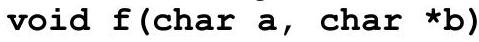
\includegraphics[max width=\textwidth]{2025_04_17_46e04c6acd873ea9558dg-187} \{char $x=a ; a=* b ; * b=x ;\}$ & \begin{tabular}{l}
procedure $f(a$ :char; var b:char); \\
var x:char; begin \( x:=a ; a:=b ; b:=x \) \\
end; \\
\end{tabular} \\
\hline
\end{tabular}
\end{center}

Dacă, înainte de apel, $\mathbf{a =}$ ' a 'şi $\mathrm{b}=$ ' b ', după executarea secvenței de program alăturate se afişează:

\begin{center}
\begin{tabular}{|l|l|l|}
\hline
Limbajul C++ & Limbajul C & Limbajul Pascal \\
\hline
$\mathrm{f}(\mathrm{a}, \mathrm{b})$; & $\mathrm{f}(\mathrm{a}$, \& b$)$; & $\mathrm{f}(\mathrm{a}, \mathrm{b})$; \\
\hline
cout<<a<<' '<<b; & printf("\%c \%c",a,b) & write (a,' ',b) ; \\
\hline
\end{tabular}
\end{center}

a) a a\\
b) b b\\
c) b a\\
d) $\mathrm{a} b$\\
e) aa\\
f) bb\\
12. Numim graf complementar al unui graf neorintat G1 graful neorientat $\mathbf{G 2} \mathbf{c u}$ aceeaşi mulţime a nodurilor ca şi G1 şi cu proprietatea că două noduri sunt adiacente în G2 dacă şi numai dacă nu sunt adiacente în G1. Dacă G1 are n noduri şi m muchii, numărul de muchii pentru G2 este:\\
a) $\operatorname{minim} \frac{n(n-1)}{2}-m$\\
b) $\operatorname{exact} \frac{\mathrm{n}(\mathbf{n}-\mathbf{1})}{2}-\mathrm{m}$\\
c) $\operatorname{maxim} \frac{\mathrm{n}(\mathrm{n}-\mathbf{1})}{2}-m$\\
d) minim $n-m$\\
e) exact $n-m$\\
f) maxim $n-m$\\
13. Subprogramul $f(a, b)$ returnează cel mai mare divizor prim al numărului natural $a$, divizor mai mic sau egal cu b ( $a \geq 3,2 \leq b \leq a$ ). Expresia care are valoarea 1 ( $\mathbf{C}++/ \mathbf{C}$ ) / True (Pascal), dacă şi numai dacă a este un număr prim este:\\
Limbajul\\
a) $f(a, a-1)==2$\\
b) $f(a, a)==2$\\
c) $f(a, a)==a$\\
C++/C\\
d) $f(a, a / 2)=a / 2$\\
e) $f(a, a)==1$\\
f) $f(a, a)=a / 2$\\
Limbajul\\
a) $f(a, a-1)=2$\\
b) $f(a, a)=2$\\
c) $f(a, a)=a$\\
Pascal:\\
d) $f(a, a \operatorname{div} 2)=$\\
e) $f(a, a)=1$\\
f) $f(a, a)=a \operatorname{div} 2$\\
14. Fie $\mathbf{G}$ un graf orientat, cu n noduri şi m arce. Dacă S 1 şi S 2 reprezintă suma gradelor interioare, respectiv exterioare ale grafului $\mathbf{G}$, afirmaţia falsă este:\\
a) $\mathrm{S} 1=\mathrm{S} 2$\\
b) $\mathrm{S} 1+\mathrm{S} 2=2 \mathrm{~m}$\\
c) dacă $\mathbf{G}$ este graf complet, atunci $\mathrm{S} 1+\mathrm{S} 2=\mathrm{n}(\mathrm{n}-1)$\\
d) $\mathrm{S} 1 \leq \mathrm{s} 2$\\
e) $\mathrm{S} 1 \geq \mathrm{S} 2$\\
f) dacă $\mathbf{G}$ este graf complet, atunci $\mathrm{S} 1+\mathrm{S} 2=\mathrm{m}(\mathrm{m}-1)$\\
15. Un arbore binar este un arbore cu rădăcină în care fiecare nod are cel mult 2 descendenți direcţi (fii). Un arbore binar complet cu n noduri are un număr de niveluri egal cu:\\
a) $\left[\log _{2} \mathrm{n}\right]-1$\\
b) $\left[\log _{2} n\right]$\\
c) $\left[\log _{2} n\right]+1$\\
d) $\left[\log _{2}(n-1)\right]$\\
e) $\left[\log _{2}(\mathrm{n}+1)\right]$\\
f) $\left[\log _{2} n\right]-1$

\section*{Varianta 35}
\begin{enumerate}
  \item Variabilele nşi c memorează numere naturale nenule. Instrucţiunea care inserează cifra c în faţa ultimei cifre a lui $n$ este:\\
Limbajul\\
a) $\mathrm{n}=(\mathrm{n} \% 10 * 10+\mathrm{c}) * 10+\mathrm{n} / 10$;\\
b) $\mathrm{n}=(\mathrm{n} / 10 * 10+\mathrm{c}) * 10+\mathrm{n} \% 10$;\\
C++/C\\
c) $\mathrm{n}=(\mathrm{n} / 10+\mathrm{c}) * 10+\mathrm{n} \% 10$;\\
d) $\mathrm{n}=\mathrm{n} / 10+\mathrm{c}+\mathrm{n} \% 10$;\\
e) $n=n / 10 * 10+c * 10+n \% 10$;\\
f) $\mathrm{n}=(\mathrm{n} \% 10+\mathrm{c}) * 10+\mathrm{n} / 10$;
\end{enumerate}

Limbajul a) $\mathrm{n}:=(\mathrm{n} \bmod 10 * 10+\mathrm{c}) * 10$\\
b) $\mathrm{n}:=(\mathrm{n}$ div $10 * 10+\mathrm{c}) * 10$

Pascal\\
+n div 10;\\
$+n \bmod 10$;\\
c) $\mathrm{n}:=(\mathrm{n}$ div $10+\mathrm{c}) * 10$\\
d) $\mathrm{n}:=\mathrm{n} \operatorname{div} 10+\mathrm{c}+\mathrm{n} \bmod 10$; +n mod 10;\\
e) $\mathrm{n}:=\mathrm{n}$ div $10 * 10+\mathrm{c} * 10$\\
f) $\mathrm{n}:=(\mathrm{n} \bmod 10+\mathrm{c}) * 10+\mathrm{n}$ div 10 ; +n mod 10;\\
2. Variabilele a şi b memorează numere naturale. Se consideră următoarea secvență de program:

\begin{verbatim}
Limbajul C++/C
b=2;
for(a=5; a<=10; a++)
{
    a=a+b;
    b=a+b;
}
cout<<a+b; |printf("%d",a+b);
\end{verbatim}

\begin{verbatim}
Limbajul Pascal
b:=2;
for a:= 5 to 10 do
begin
    a:=a+b;
    b:=a+b
end;
write(a+b);
\end{verbatim}

În urma executării secvenței de program alăturate se afişează:\\
a) 18\\
b) 26\\
c) 28\\
d) 44\\
e) 48\\
f) 52\\
3. Variabilele i,j şi k memorează numere naturale. Se consideră următoarea secvenţă de program:

\begin{verbatim}
Limbajul C++/C
for(i=1;i<=10;i++)
{ for(j=1;j<=i;j++)
        cout<<j; |printf("%d",j) ;
    for(k=9;k>0;k--)
        cout<<k; |printf("%d",k) ;
}
\end{verbatim}

\begin{verbatim}
Limbajul Pascal
for i:=1 to 10 do
begin
        for j:=1 to i do write(j);
        for k:=9 downto 1 do
            write(k)
    end;
\end{verbatim}

Numărul de execuţii ale instrucțiunii care afişează valoarea variabilei $k$ este:\\
a) 495\\
b) 90\\
c) 60\\
d) 55\\
e) 10\\
f) 9\\
4. Pentru un graf neorientat cu 9 muchii şi 12 noduri, numărul minim de componente conexe este:\\
a) 1\\
b) 2\\
c) 3\\
d) 4\\
e) 5\\
f) 6\\
5. Algoritmul lui Euclid este utilizat pentru:\\
a) calculul numărului de multipli ai unui număr natural;\\
b) descompunerea în factori primi a unui număr natural;\\
c) calculul celui mai mare divizor comun a două numere naturale;\\
d) calculul numărului de divizori ai unui număr natural;\\
e) suma divizorilor unui număr natural;\\
f) suma divizorilor proprii ai unui număr natural.\\
6. Variabilele $\mathbf{x}, \mathbf{y}, \mathbf{z}, \mathbf{s}$ şi $\mathbf{p}$ memorează numere reale. Se consideră următoarea secvență de program:

Limbajul C++/C\\
if $(x>y)$ if $(y>z)$ if $(z>x)$\\
$s=x+y+z ; ~ e l s e ~ p=x * y * z ; ~$

\section*{Limbajul Pascal}
if $x>y$ then if $y>z$ then if $z>x$ then $\mathrm{s}:=\mathrm{x}+\mathrm{y}+\mathrm{z}$ else $\mathrm{p}:=\mathrm{x} \mathrm{K}^{\mathrm{y}} \mathrm{z}_{\mathrm{z}}$;

Secvenţa de program echivalentă cu ea, care să conţină o singură instrucţiune de decizie, este:\\
Limbajul\\
a) if $(x>y$ || $y>z) s=x+y+z$;\\
b) if( $x>y \& \& y>z) s=x+y+z$;\\
C++/C\\
c) if $(x>y \& \& y>z) s=x+y+z$;\\
d) if( $x>y \& \& y>z) p=x * y * z$;\\
e) if $(x>y \& \& y>z) s=x+y+z$;\\
f) if( $x>y$ || $y>z) p=x * y * z$;\\
else $p=p^{*} y^{*} z$;\\
Limbajul\\
Pascal\\
a) if ( $x>y$ ) or ( $y>z$ ) then $\mathrm{s}:=\mathrm{x}+\mathrm{y}+\mathrm{z}$;\\
c) if ( $x>y$ ) and ( $y>z$ ) then $\mathrm{s}:=\mathrm{x}+\mathrm{y}+\mathrm{z}$;\\
e) if ( $x>y$ ) and ( $y>z$ ) then\\
$\mathrm{s}:=\mathrm{x}+\mathrm{y}+\mathrm{z}$\\
else $p:=p * y^{*} z ;$\\
b) if ( $x>y$ ) and ( $y>z$ ) then $s:=x+y+z$;\\
d) if ( $x>y$ ) and ( $y>z$ ) then $p:=x * y^{*} z$;\\
f) if $(x>y)$ or $(y>z)$ then $p:=x * y * z$;\\
7. Numărul de interschimbări care se efectuează în cazul sortării descrescătoare a şirului de numere consecutive $0,1,2,3, \ldots, 8,9,10$ prin metoda bulelor este:\\
a) 0\\
b) 10\\
c) 11\\
d) 45\\
e) 55\\
f) 121\\
8. Fie a un tablou bidimensional cu 45 linii (numerotate de la 1 la 45) şi 45 coloane (numerotate de la 1 la 45). Expresia care calculează numărul de ordine al elementului de pe linia i şi coloana j (a câta valoare este acesta, pornind din colţul din sânga sus, de la prima spre ultima linie, pe fiecare linie elementele numărându-se de la stânga la dreapta) este:\\
a) $i * 45+j-1$\\
b) $(i-1) * 45+j$\\
c) $(j-1) * 45+i$\\
d) $j * 45+i-1$\\
e) $(i+1) * 45+j$\\
f) $(j+1) * 45+i$\\
9. Se consideră algoritmul care determină toate permutările distincte de n obiecte (numerotate de la 1 la $n$ ), în care pe orice poziţie de rang par se află o valoare pară. De exemplu, pentru $\mathrm{n}=5$, primele trei permutări generate în ordine lexicografică sunt: $(1,2,3,4,5),(1,2,5,4,3),(1,4,3,2,5)$.\\
Pentru $n=4$, numărul total de astfel de permutări este:\\
a) 12\\
b) 10\\
c) 8\\
d) 7\\
e) 6\\
f) 4\\
10. Subprogramul $f$ primeşte prin parametrii $a$ şi $b$ două valori întregi ( $a \leq b$ ) şi returnează numărul de numere prime din intervalul închis [a,b]. Expresia care are valoarea 1 $(\mathbf{C}++/ \mathbf{C}) /$ True (Pascal), numai dacă valoarea întreagă $\mathbf{x}(\mathbf{x}>5)$ este număr prim este:\\
a) $f(x-1, x)==f(x, x+1)$\\
b) $f(x, x)==1$

\begin{center}
\begin{tabular}{lll}
Limbajul & c) $f(2, x)!=f(2, x-1)$ & d) $f(2, x)!=f(2, x+1)$ \\
$C++/ C$ & e) $f(2, x)==f(2, x-1)$ & f) $f(2, x)==f(2, x+1)$ \\
\end{tabular}
\end{center}

Limbajul\\
a) $f(x-1, x)=f(x, x+1)$\\
b) $f(x, x)=1$

Pascal\\
c) $f(2, x)<>f(2, x-1)$\\
d) $f(2, x)<>f(2, x+1)$\\
e) $f(2, x)=f(2, x-1)$\\
f) $f(2, x)=f(2, x+1)$\\
11. Se consideră următoarea secvenţă de program:

\begin{verbatim}
    Limbajul C++
int a,b;
void f(int x,int &y)
{int b=x;y+=b;x=y;}
int main()
{ a=20;b=23;
    f(a,b) ;
    cout<<a<<' '<<b;
    return 0;
}
\end{verbatim}

\begin{verbatim}
Limbajul C
int a,b;
void f(int x,int *y)
{int b=x;*y=*y+b;x=*y;}
int main()
{ a=20;b=23;
    f(a,&b) ;
    printf("%d %d",a,b);
    return 0;
}
\end{verbatim}

\begin{verbatim}
Limbajul Pascal
var a,b:integer;
procedure
f(x:integer; var
y:integer);
var b:integer;
begin b:=x;y:=y+b;x:=y
end;
begin
    a:=20;b:=23;
    f(a,b) ;write(a,' ',b)
end.
\end{verbatim}

În urma executării secvenței de program alăturate se afişează:\\
a) $43 \quad 43$\\
b) 2323\\
c) 2023\\
d) $23 \quad 43$\\
e) 2043\\
f) 2320\\
12. Numărul minim de muchii care trebuie adăugate grafului din figura alăturată, astfel încât acesta să devină eulerian este:\\
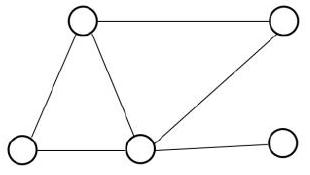
\includegraphics[max width=\textwidth, center]{2025_04_17_46e04c6acd873ea9558dg-191}\\
a) 0\\
b) 1\\
c) 2\\
d) 3\\
e) 4\\
f) 5\\
13. Subprogramul minim returnează cifra minimă a unui număr natural. Pentru o variabilă $\mathbf{x}$, ce memorează o valoare naturală de cel mult 2 cifre, subprogramul este apelat într-o secvență de forma Limbajul C++/C: if (minim $\left.\left.(\mathbf{x})+\operatorname{minim}\left(\mathbf{x}^{*} \mathbf{x} * \mathbf{x}\right)\right)==0\right) \mathrm{nr}++$; Limbajul Pascal: if minim(x)+minim $\left(x^{*} x^{*} x\right)=0$ then $n r:=n r+1$;\\
Varianta pentru un antet corect al subprogramului este:\\
Limbajul C++/C\\
a) int minim(long $u$ )\\
b) int minim(long $x * x^{\star}$ )\\
c) int minim(int $x$, int $y$ )\\
d) void minim(long $u$ )\\
e) void minim(int $x$, int $y$ )\\
f) void minim(long $x^{\star} x^{\star} x$ )\\
Limbajul Pascal\\
a) function minim(u:longint) :integer;\\
b) function minim ( $x^{*} x^{*} x$ :longint) :integer;\\
c) function minim( $x, y$ :integer) :integer;\\
d) procedure minim(u:longint);\\
e) procedure minim ( $x, y$ : longint) ;\\
f) procedure minim ( $\mathbf{x}^{*} \mathbf{x}^{*}$ : longint);\\
14. Un arbore binar este un arbore cu rădăcină în care fiecare nod are cel mult 2 descendenţi direcţi (fii).\\
Un arbore binar complet, cu h niveluri, are un număr de noduri egal cu:\\
a) 2 h\\
b) $2 \mathrm{~h}+1$\\
c) $2 \mathrm{~h}-1$\\
d) $2^{\mathrm{h}}-1$\\
e) $2^{\text {h }}$\\
f) $2^{\mathrm{h}}+1$\\
15. Fie G un graf neorientat, cu n noduri şi p componente conexe. Numărul maxim de muchii este:\\
a) $\frac{\mathrm{n}(\mathrm{n}-1)}{2}$\\
b) $\frac{(\mathbf{n}-\mathbf{p})(\mathrm{n}-\mathrm{p}+1)}{2}$ c) $\frac{\mathrm{n}(\mathrm{n}+1)}{2}$\\
d) $\frac{(\mathbf{n}+\mathbf{p})(\mathrm{n}+\mathrm{p}+\mathbf{1})}{2}$\\
e) $\frac{p(p-1)}{2}$\\
f) $\frac{p(p+1)}{2}$

\section*{Varianta 36}
\begin{enumerate}
  \item Variabilele $\mathbf{x}$ și $\mathbf{y}$ memorează numere întregi. Se consideră următoarea secvenţă de program:
\end{enumerate}

$$
\begin{array}{cl}
\text { Limbajul } & x=2020 / 7 ; \\
\text { C++/C } & y=123 \% 10 * 3 / 8 ; \\
& \text { cout<<x<<' '<<y } \\
& \text { |printf("\%d } \\
& \text { \%d", } x, y) ;
\end{array}
$$

\begin{verbatim}
Limbajul x:=2020 div 7;
    Pascal y:=123 mod 10*3 div 8;
        write(x,' ',y);
\end{verbatim}

După executarea secvențe de program alăturate, variabilele $\mathbf{x}$ și $\mathbf{y}$ au valorile:\\
a) 660\\
b) 661\\
c) 2020\\
d) 2021\\
e) 2880\\
f) 2881\\
2. Se consideră următoarea expresie:

\section*{Limbajul C++/C: $\quad(x==y)==(y==z) \quad$ Limbajul Pascal: $\quad(x=y)=(y=z)$}
Expresia dată are valoarea $0(\mathbf{C}++/ \mathbf{C}) /$ False(Pascal) dacă și numai dacă cele trei variabile întregi $\mathbf{x}, \mathrm{y}$ și $\mathbf{z}$ sunt:\\
a) toate trei egale\\
b) neinițializate\\
b) neinițializate\\
Limbajul C++/C\\
c) $(x==y \& \& y!=z) \|(x!=y \& \& y==z)$\\
d) $(x==y \& \& y!=z) \& \&(x!=y \& \&$\\
$y==z)$\\
e) $(x==y \quad y!=z) \|(x!=y \quad y==z)$\\
f) $(x==y$ || $y!=z) \& \&(x!=y$ || $\mathrm{y}=\mathrm{z}$ )

Limbajul Pascal\\
c) $(x=y$ and $y<>z)$ or ( $x<>y$ and $y=z$ )\\
d) ( $x=y$ and $y<>z$ ) and ( $x<>y$ and $y=z$ )\\
e) $(x=y$ or $y<>z$ ) or ( $x<>y$ or $y=z$ )\\
f) ( $x=y$ or $y<>z$ ) and ( $x<>y$ or $y=z$ )\\
3. Variabilele de tip întreg $\mathbf{x}$ și $\mathbf{y}$, inițial egale, memorează valoarea 100 . Se consideră următoarea secvenţă de program:

\begin{displayquote}
Limbajul C++/C if $(x>y) \quad \begin{aligned} & x=10 \star y-8 * x ; \\ & \text { else } y=10 * x-8 * y ;\end{aligned}$\\
Limbajul Pascal\\
if $x>y$ then $x:=10 * y-8 * x$\\
else $y:=10 * x-8 * y$;
\end{displayquote}

În urma executării secvenței de program alăturate, diferența absolută dintre valorile celor două variabile este:\\
a) -200\\
b) -100\\
c) 0\\
d) 1\\
e) 100\\
f) $\mathbf{2 0 0}$\\
4. Se consideră următoarele două secvențe:

\begin{verbatim}
Limbajul C++/C
while ...... do
{ { cout<<"20";
    a=a-1; a--;
    cout<<"20"; }while(a>=1);
}
\end{verbatim}

\begin{verbatim}
Limbajul Pascal
while ..... do repeat
begin write('20');
    a:=a-1; a:=a-1;
    write('20'); until a<1;
end;
\end{verbatim}

Variabila de tip întreg a are inițial valoarea 21 . Cele două secvenţe sunt echivalente dacă punctele de suspensie se înlocuiesc cu:\\
a) $a=0$\\
b) $a>0$\\
c) $a>=1$\\
d) $a>1$\\
e) $a<=1$\\
f) $a<1$\\
5. Se consideră următorul subprogram:

\begin{verbatim}
        Limbajul C++/C
int f(int x)
{
    if(x) return 2*f(x-1);
    else return 3;
}
\end{verbatim}

\begin{verbatim}
Limbajul Pascal
function f(x:integer):integer;
begin
    if x<>0 then f:=2*f(x-1);
    else f:=3
end;
\end{verbatim}

Valoarea returnată de apelul $\pounds(5)$ pentru funcţia alăturată este:\\
a) 3\\
b) 13\\
c) 48\\
d) 96\\
e) 144\\
f) $\mathbf{1 6 2}$\\
6. Concatenarea a două șiruri de caractere se poate realiza cu funcţia predefinită:\\
Limbajul a)\\
b)\\
c) strlen\\
d) strcat e)\\
f) $\operatorname{strlwr}$\\
C++/C strconcat strcmp\\
strst $r$\\
Limbajul a) paste\\
b) copy\\
c) length\\
d) concat e) str\\
f) pos\\
Pascal\\
7. Se consideră un graf neorientat cu nodurile numerotate de la 1 la 5 și muchiile $[1,2],[1,5],[2,3],[2,4],[2,5],[3,4],[4,5]$. Numărul lanțurilor distincte de lungime $\mathbf{3}$ de la nodul 1 la 4 este:\\
a) 3\\
b) 4\\
c) 5\\
d) 6\\
e) 7\\
f) 8\\
8. Se consideră un arbore cu rădăcină, cu 2020 noduri. Numărul minim de frunze pe care îl poate avea arborele este:\\
a) 0\\
b) 1\\
c) 2\\
d) 1010\\
e) 2019\\
f) $\mathbf{2 0 2 0}$\\
9. Utilizând metoda backtracking se generează toate numerele, de cel mult trei cifre, formate cu cifre distincte, care au suma cifrelor egală cu 7 și nu sunt divizibile cu 10. Astfel, se generează în această ordine numerele: 106, 124, 142, 16, 205, .... Folosind acceași metodă se generează toate numerele naturale cu cifre distincte, care au suma cifrelor egală cu 9 și nu sunt divizible cu 5 . Al șaselea număr generat este:\\
a) 135\\
b) 153\\
c) 162\\
d) 207\\
e) 216\\
f) 234\\
10. Se consideră următoarea secvență de program în care toate variabilele sunt numere întregi:

\begin{verbatim}
Limbajul C++/C
for (i=0;i<= 2020;i++) for i:=0 to 2020 do
    { =i+1;a[i]=t;t--; } begin t:=i+1;a[i]:=t;dec(t); end;
Suma elementelor tabloului a este:
\end{verbatim}

a) 2020\\
b) 2021\\
c) 4040\\
d) 4041\\
e) 2041210\\
f) 2043231\\
11. Folosind metoda bulelor tabloul unidimensional (5,6,10,20,1) este ordonat crescător: $(1,5,6,10,20)$. Numărul de parcurgeri necesare pentru a ordona crescător tabloul este:\\
a) 9\\
b) 8\\
c) 7\\
d) 6\\
e) 5\\
f) 4\\
12. Un număr $\overline{\mathbf{a b c}}$ se numește excepțional dacă $\mathbf{b}=\mathbf{a}^{c}$. Mulțimea numerelor excepționale conține un număr de valori egal cu:\\
a) 36\\
b) 29\\
c) 26\\
d) 15\\
e) 6\\
f) 5\\
13. Se consideră următorul subprogram:

\begin{verbatim}
Limbajul
C++/C
void f(int n)
{
    int i;
    if(n>0) for(i=1;i<=n;i++)
    { f(n-2);
        cout<<i<<' ';
            lprintf("%d ",i);
    }
}
\end{verbatim}

\begin{verbatim}
Limbajul Pascal
procedure f (n:integer);
var i:integer;
begin
if n>0 then
    for i:=1 to n do
        begin
        f(n-2);write(i,' ')
        end
end;
\end{verbatim}

Valoarea lui $n$ pentru care sunt afișate valorile 111213 la apelul $f(n)$ este:\\
a) 12\\
b) 9\\
c) 6\\
d) 5\\
e) 4\\
f) 3\\
14. Variabila a memorează elementele unui tablou bidimensional cu 5 linii şi 5 coloane, numerotate de la 1 la 5, iar celelalte variabile sunt de tip întreg. Specificaţi care va fi conţinutul variabilei a în urma executării secvenței de program date, dacă

\begin{center}
\begin{tabular}{lllll}
1 & 2 & 3 & 4 & 5 \\
1 & 2 & 3 & 4 & 5 \\
1 & 2 & 3 & 4 & 5 \\
1 & 2 & 3 & 4 & 5 \\
1 & 2 & 3 & 4 & 5 \\
\end{tabular}
\end{center} tabloul bidimensional are inițial conținutul alăturat:

\begin{verbatim}
Limbajul C++/C
for(i=1; i<=n; i++)
if(i<=n/2)
for(j=1;j<=i;j++)
{aux=a[i][j];
    a[i][j]=a[i][n-j+1];
    a[i][n-j+1]=aux;
}
else
    for(j=1;j<=n-i+1;j++)
{ aux=a[i][j];
        a[i][j]=a[i][n-j+1];
        a[i][n-j+1]=aux;
}
\end{verbatim}

a)

\begin{center}
\begin{tabular}{lllllllllllllllllllllllllllllll}
5 & 4 & 3 & 2 & 1 & 5 & 4 & 3 & 2 & 1 & 5 & 2 & 3 & 4 & 1 & 1 & 2 & 5 & 4 & 3 & 1 & 2 & 3 & 5 & 4 & 1 & 2 & 3 & 4 & 5 &  \\
5 & 2 & 3 & 4 & 1 & 1 & 2 & 3 & 4 & 5 & 5 & 4 & 3 & 2 & 1 & 1 & 2 & 5 & 4 & 3 & 1 & 2 & 3 & 5 & 4 &  & 1 & 2 & 3 & 4 & 5 \\
5 & 2 & 3 & 4 & 1 & 1 & 2 & 3 & 4 & 5 & 5 & 4 & 3 & 2 & 1 & 1 & 2 & 5 & 4 & 3 & 1 & 2 & 3 & 5 & 4 & 1 & 2 & 3 & 4 & 5 &  \\
5 & 2 & 3 & 4 & 1 & 1 & 2 & 3 & 4 & 5 & 5 & 4 & 3 & 2 & 1 & 1 & 2 & 5 & 4 & 3 & 1 & 2 & 3 & 5 & 4 & 1 & 2 & 3 & 4 & 5 &  \\
5 & 4 & 3 & 2 & 1 & 5 & 4 & 3 & 2 & 1 & 5 & 2 & 3 & 4 & 1 & 1 & 2 & 5 & 4 & 3 &  & 1 & 2 & 3 & 5 & 4 &  & 1 & 2 & 3 & 4 \\
\end{tabular}
\end{center} 5

\begin{enumerate}
  \setcounter{enumi}{14}
  \item Se consideră următorul subprogram:
\end{enumerate}

\begin{verbatim}
    Limbajul C++/C
int T(int n)
{
\end{verbatim}

\begin{verbatim}
                Limbajul Pascal
function T(n:integer):integer;
var 0,m,c:integer;
\end{verbatim}

\begin{verbatim}
    int 0,m=n, c=1;
    o=n;
    while(o>9)
    { c=c*10;
        o=o/10;
    }
    o=n%c*10+n/c;
    while(o!=n)
        {
            if(m<0) m=0;
            O=0%c*10+o/c;
        }
        return m;
}
\end{verbatim}

\begin{verbatim}
begin
    m:=n; c:=1;0:=n;
    while(o>9) do
        begin
            c:=c*10; 0:=0 div 10;
        end;
    o:=n mod c*10+n div c;
    while o<>n do
        begin
                if m<0 then m:=0;
                o:=0 mod c*10 + o div c;
        end;
    T:=m;
end;
\end{verbatim}

Știind că parametrul formal $n$ este un număr natural format din 3 cifre, subprogramul $T$ poate returna un număr de valori cu cifra sutelor 9 egal cu:\\
a) 100\\
b) 200\\
c) 225\\
d) 252\\
e) 260\\
f) 261

\section*{Varianta 37}
\begin{enumerate}
  \item Se consideră următoarea secvenţă de program:
\end{enumerate}

\begin{verbatim}
Limbajul C++/C
char c='7';
float a= c- '9';
cout<<a; | printf("%.Of",a);
\end{verbatim}

\begin{verbatim}
Limbajul Pascal
var c:char; a:real;
c:='7';
a:=ord(c)- ord('9');
write(a:1:0);
\end{verbatim}

Valoarea afișată în urma executării secvenței de program alăturate este:\\
a) 79\\
b) -2\\
c) 2.0\\
d) 2\\
e) '79'\\
f) -16\\
2. Se consideră următoarea listă de descendenți asociată unui arbore cu rădăcină cu 8 noduri:

\begin{verbatim}
1: 4,7,6,2
2: -
3: 4,6,5,2,7,8,1
4: -
5: -
6: -
7: 2
8: 7,2,4,1,6
\end{verbatim}

Varianta care reprezintă vectorul de taţi asociat acestui arbore este:\\
a) 23813180\\
b) 87018113\\
c) 87013113\\
d) 03183111\\
e) 87813110\\
f) 07831331\\
3. În matricea de adiacență asociată unui graf neorientat cu $\mathbf{n}$ noduri, numărul de cifre de 1 aflate sub diagonala principală este egal cu $n \star(n-1) / 2$. Numărul de muchii ce trebuie adăugate la acest graf astfel încât acesta să devină complet este:\\
a) $n-1$\\
b) n\\
c) 1\\
d) $(\mathrm{n}-1) / 2$\\
e) $\mathrm{n} / 2$\\
f) 0\\
4. Se consideră un graf neorientat cu 3675 de noduri și 10589 muchii. Gradul maxim pe care îl poate avea un nod din reprezentarea grafului ce conține un număr maxim de noduri izolate este:\\
a) 147\\
b) 148\\
c) 146\\
d) 3666\\
e) 3674\\
f) 145\\
5. Şirul de caractere s ce desemnează o propoziție cu exact 11 cuvinte formate doar din litere mici, mari și separate prin câte un spațiu. Se consideră următoarea secvență de program:

\begin{verbatim}
        Limbajul C++/C
int n;
char s[100], *p, c[100];
strcpy(s,s+(strchr(s,' ')-s));
p=strtok(s," ");
while (p && n)
        { p=strtok(NULL," ");
            strcpy(c, p);
            n--;
    }
\end{verbatim}

\begin{verbatim}
Limbajul Pascal
var s,c,p:string[100];n:integer;
delete(s,1,pos(' ',s));
while n<>0 do
    begin
        delete(s,1,pos(' ',s));
        c:=copy(s,1,pos(' ',s)-1);
        n:=n-1
    end;
\end{verbatim}

Pentru a memora în variabila c cuvântul din mijloc, valoarea atribuită variabilei $n$ este:\\
a) 11\\
b) 6\\
c) 5\\
d) 7\\
e) 3\\
f) 4\\
6. Se consideră șirul: $1,1,2,1,2,3,1,2,3,4,1,2,3,4,5,1,2,3,4,5,6,1,2,3,4$, $5,6,7 \ldots$ şi următoarea secvenţă de program:

\begin{verbatim}
Limbajul C++/C
int $n, k, s=0$;
cin>>n; | scanf("\%d",\&n);
$\mathrm{k}=1$;
while( $s<n$ )
\{ $\mathrm{s}=\mathrm{s}+\mathrm{k} ; \mathrm{k}++$; \}
\end{verbatim}

\begin{verbatim}
Limbajul Pascal
var n,k,s:integer;
$\operatorname{read}(\mathrm{n}) ; \mathrm{k}:=1$; $\mathrm{s}:=0$;
while $s<n$ do
    begin
        s:=s+k; inc(k)
    end;
\end{verbatim}

Expresia care determină termenul de pe o anumită poziție n dată de la tastatură, dacă numerotarea termenilor pleacă de la valoarea 1 este:\\
a) $s-(k-n)+1$\\
b) $k-s+n-1$\\
c) $k-s+n$\\
d) $k+s-n$\\
e) $n-k$\\
f) $k+n$\\
7. Se consideră următoarea secvență de program:

\begin{verbatim}
            Limbajul C++/C
int i, j, n, a[10][10];
cin>>n; |scanf("%d",&n);
for (i=1;i<=n;i++)
    for (j=1;j<=n-i+1;j++)
        {
            a[i][j]=i+j;
            a[n-j+1][n+1-i]=i+j;
        }
\end{verbatim}

\begin{verbatim}
Limbajul Pascal
var a: array [1..10, 1..10] of integer;
    i, j, n: byte;
read(n);
for i:=1 to n do
        for j:=1 to n-i+1 do
            begin
                a[i][j]:= i+j;
                a[n-j+1][n+1-i]:=i+j
            end;
\end{verbatim}

În urma executării secvenței de program alăturate se obține:\\
a) un tablou bidimensional cu elementele simetrice față de diagonala principală dar nu şi faţă de diagonala secundară;\\
b) un tablou bidimensional cu elementele simetrice față de diagonala secundară dar nu şi faţă de diagonala principală;\\
c) un tablou bidimensional cu elementele simetrice atât față de diagonala principală cât şi faţă de diagonala secundară;\\
d) un tablou bidimensional cu elementele identice pe coloane;\\
e) un tablou bidimensional cu elementele identice pe linii;\\
f) un tablou bidimensional cu toate elementele egale între ele.\\
8. Variabilele $\mathbf{a}, \mathbf{b}, \mathrm{i}$ și d memorează numere naturale. Se consideră următoarea secvență de program:

\begin{verbatim}
Limbajul C++/C
for(i=a*b;i>=b;i--)
    if(i%a==0 && i%b==0)
            d=i;
cout<<d; | printf("%d",d);
\end{verbatim}

\begin{verbatim}
Limbajul Pascal
for i:= a*b downto b do
    if i mod a=0 and i mod b=0 then
        d:=i;
write(d);
\end{verbatim}

Valoarea afișată în urma executării secvenței de program alăturate reprezintă:\\
a) cel mai mare divizor comun\\
b) numărul de multiplii comuni\\
c) cel mai mic multiplu comun\\
d) numărul de divizori comuni\\
e) cel mai mare multiplu comun\\
f) numărul de divizori al produsulu $\mathbf{a * b}$\\
9. Se consideră următoarea secvență de program:

\begin{verbatim}
        Limbajul C++/C
int a,i,c;
cin>>a; | scanf("%d",&a);
c=0;
for (i=1;i<=a;i++)
        if (i%5==0)
            { int j=i;
                while (j%5==0)
                { c++; j=j/5; }
            }
    cout<<c; | printf("%d",c);
\end{verbatim}

\section*{Limbaju Pascal}
\begin{verbatim}
var a,i,c,j:integer;
read(a) ; c:=0;
for $i:=1$ to a do
    if i mod 5=0 then
        begin
            j:=i;
            while j mod 5=0 do
                begin
                    c:=c+1; j:=j div 5
                    end
        end;
write(c);
\end{verbatim}

Valoarea afișată în urma executării secvenței de program alăturate reprezintă:\\
a) factorialul numărului $a$;\\
b) numărul cifrelor cu valoarea 0 de la sfârșitul factorialului numărului a;\\
c) puterea lui 5 din factorialul numărului $a$;\\
d) atât puterea lui 5 din factorialul numărului a, cât și numărul cifrelor cu valoarea 0 de la sfârșitul acestui factorial;\\
e) numărul de elemente divizibile cu 5 mai mici decat a;\\
f) numărul de elemente divizibile cu 10 mai mici decat a.\\
10. Se consideră următoarea secvență de program:

\begin{verbatim}
        Limbajul C++/C
struct oras {
    char strada[101];
    unsigned nr,cod_postal;
};
struct colet {
    char destinatar[51];
    struct oras adresa;
};
struct colet v[100];
\end{verbatim}

\begin{verbatim}
Limbajul Pascal
type oras= record
        strada: string[101];
        nr, cod_postal: word
    end;
    colet= record
        destinatar: string[50];
        adresa: oras
    end;
var v: array [1..101] of colet;
\end{verbatim}

Varianta care reprezintă o accesare corectă a unei litere din numele unei străzi corespunzătoare unui colet transmis de o anumită firmă de curierat este:\\[0pt]
a) v[5]. adresa.oras [1]\\[0pt]
b) v [5] . adresa [1] .strada\\
C) $\mathrm{v}[5]$. adresa. strada [1]\\[0pt]
d) v.colet.strada [5]\\[0pt]
e) adresa.v[5].strada [1]\\[0pt]
f) v .strada[1] .adresa\\
11. Fişierul examen.txt conţine pe prima linie a sa valoarea unui număr natural $n$ mai mic decât 100, iar pe următoarea linie $n$ valori întregi separate prin câte un spaţiu. Se consideră următoarea secvență de program:

\section*{Limbajul C++/C}
\section*{Limbajul Pascal}
\begin{verbatim}
ifstream f("examen.txt"); | | var f,g:text; n,i:byte;
FILE *f; f= fopen("examen.txt","r"); v: array [1..100] of integer;
\end{verbatim}

\begin{verbatim}
int n, i, v[100];
f>>n; |fscanf(f,"%d",&n);
for (i=1;i<=n;i++) f>>v[i];
            |fscanf(f,"%d",&v[i]);
f.close();|fclose(f);
ifstream g("examen.txt"); |
FILE *g; g= fopen("examen.txt","r");
for (i=2;i<=n;i++) g>>v[i];
        |fscanf(g,"%d",&v[i]);
g.close(); | fclose(g);
cout<<v[n]; |printf("%d",v[n]);
\end{verbatim}

\begin{verbatim}
assign(f,'examen.txt');
reset(f);
readln(f,n);
for i:= 1 to n do
    read(f,v[i]);
close(f);
assign(g,'examen.txt');
reset(g);
for i:= 2 to n do
    read(g,v[i]);
close(g); write(v[n]);
\end{verbatim}

Valoarea afișată în urma executării secvenței de program alăturate reprezintă:\\
a) prima valoare din fișier;\\
b) penultima valoare din fișier;\\
c) antepenultima valoare din fișier;\\
d) ultima valoare din fișier;\\
e) numărul de valori din fișier;\\
f) a doua valoare din fișier.\\
12. Se consideră următoarea secvență de program:

\begin{verbatim}
Limbajul C++/C
unsigned n;
int c;
float f(int n)
{ if (n)
    { c++; return (n%10+ f(n/10));}
    else return 0;
}
\end{verbatim}

\begin{verbatim}
Limbajul Pascal
var n:word; c:integer;
function f(n: integer): real;
begin
    if n<>0 then
        begin
            inc(c);
            f:= n mod 10+ f(n div 10)
        end
        else f:= 0
end;
\end{verbatim}

Apelul corect al funcției care returnează media aritmetică a cifrelor numărului natural $n$ este:\\
a) $f(n) / c$\\
b) $f(c)$\\
c) $f(n / c)$\\
d) $f(n)$\\
e) $f(c) / n$\\
f) $f(c / n)$\\
13. Se consideră următoarea secvență de program:

\section*{Limbajul C++/C}
\begin{verbatim}
char s[101]="Sebastian
Nicholas", p[50]="bytes to mb";
strcpy(s+ (strchr(s,'a')+1 -s),
s+ strlen(s)-1);
s[3]++;
strncpy (s+3,p,2);
cout<<s<<endl;
    |printf("%s\n",s);
\end{verbatim}

\section*{Limbajul Pascal}
\begin{verbatim}
var s, p: string[100];
s:='Sebastian Nicholas';
p:='bytes to mb';
delete(s,pos('a',s)
    + 2,length(s)-1);
s[4]:=chr(ord(s[4])-1);
delete(s, length(s)-1,2);
s:=s+ p[1]+ p[2];
writeln(s);
\end{verbatim}

În urma executării secvenței de program alăturate se afișează:\\
a) Sebyy\\
b) Sebabby\\
c) Nicholas\\
d) Sebaty\\
e) Sebby\\
f) Seba\\
14. Variabila n memorează un număr natural şi variabila a memorează un tablou bidimensional pătratic cu n linii şi n coloane numerotate de la 1 la n . Se consideră următoarea secvență de program:

\begin{verbatim}
for (k=1;k<=n/2+1;k++) {
    for (j=k;j<=n-k+1;j++)
        cout<<a[k][j]<<' ';
            | printf("%d ",a[k][j]);
    for (i=k+1;i<=n-k+1;i++)
        cout<<a[i][n-k+1]<<' ';
            |printf("%d ",a[i][n-k+1]);
    for (j=n-k;j>=k;j--)
        cout<<a[n-k+1][j]<<' ';
            | printf("%d ",a[n-k+1][j]);
    for (i=n-k;i>k;i--)
        cout<<a[i][k]<<' ';
            |printf("%d ",a[i][k]);
}
\end{verbatim}

În urma executării secvenței de program alăturate se vor afişa:\\
a) elementele tabloului pe coloane, de la ultima la prima coloană;\\
b) elementele tabloului în spirală;\\
c) elementele tabloului pe linii, de la prima la ultima linie;\\
d) elementele tabloului pe diagonale;\\
e) elementele tabloului aflate pe coloane impare;\\
f) elementele tabloului ce nu se află pe vreuna din cele două diagonale.\\
15. Nicholas are la Informatică un număr de m note stocate în tabloul unidimensional note, iar în variabila teza este trecut rezultatul obținut de el la lucrarea de sfârșit de semestru. Se știe că media se încheie cu un număr de $n$ note $(\mathbf{m}<\mathbf{n})$, iar Nicholas dorește sa obțină media finală x.\\
Folosind metoda backtracking, Nicholas a creat un program care îi generează în tabloul unidimensional note, în continuarea celor m note existente, restul de m-n note necesare încheierii mediei. S-a notat cu $\mathbf{k}$ poziția pe care se generează pe rând restul notelor.\\
În rezolvarea programului s-a utilizat funcția medie al cărei apel calculează media curentă. Se consideră următoarea secvență de program:

\section*{Limbajul C++/C}
\begin{verbatim}
float note[10], teza;
int n,m,k,as,ev,i,x;
float medie(float note[10],int m)
{ float s=0;
    for (i=1;i<= m;i++)
        s=s+note[i];
    return (3*s+m*teza)/(4*m);
}
valid(float note[10],int k,int ev)
| void valid(float note[10],
int k,int *ev)
void
{
    ev=1; |*ev=1;
    if (k>m+1)
        if (note[k]< note[k-1])
            ev=0; l*ev=0;
    if (k==n)
            if (...)
\end{verbatim}

\begin{verbatim}
for k:= 1 to n div 2+ 1 do
begin
    for j:=k to n-k+1 do
        write(a[k,j], ' ');
    for i:=k+1 to n-k+1 do
        write(a[i,n-k+1],' ');
    for j:=n-k downto k do
        write(a[n-k+1][j],' ');
    for i:=n-k downto k+1 do
        write(a[i,k],' ');
end;
\end{verbatim}

\section*{Limbajul Pascal}
\begin{verbatim}
type sir= array [1..11] of byte;
var note: sir;
    m,n,teza,k,i x:word;
    as,ev:boolean;
function
medie (note:sir;m:word) : real;
var s:word;
begin
    s:=0;
    for i:=1 to m do s:=s+note[i];
    medie:=(3*s+m*teza)/(4*m)
end;
procedure valid( note:sir;k word;var
ev:boolean);
begin
    ev:=true;
    if k>m+1 then
        if note[k]< note[k-1] then
            ev:=false;
\end{verbatim}

\begin{verbatim}
    ev=0; |*ev=0;
}
\end{verbatim}

\begin{verbatim}
    if k=n then
        if ... then ev:=false
end;
\end{verbatim}

Pentru ca programul să genereze toate combinațiile de note de care Nicholas are nevoie pentru a obține media dorită, expresia corespunzătoare punctelor de suspensie din secvenţa de program este:\\
a) Limbajul C++/C: medie (note, $n$ ) ! $=x$;

Limbajul Pascal: medie (note, n) <>x\\
b) Limbajul C++/C: medie (note, $n$ ) $<=(x-0.5) \& \&$ medie (note, $n$ ) $>(x+0.5)$

Limbajul Pascal: medie (note, $n$ ) $<=(x-0.5)$ and medie (note, $n$ ) $>(x+0.5)$\\
c) Limbajul C++/C: medie (note, $n$ ) $<(x-0.5$ ) || medie (note, $n$ ) $>$ ( $x+0.5$ )

Limbajul Pascal: medie (note, $n$ ) $<(x-0.5$ ) or medie (note, $n$ ) $>$ ( $x+0.5$ )\\
d) Limbajul C++/C: medie (note, n) $>=(x-0.5) \& \&$ medie (note, $n$ ) $<=(x+0.5)$

Limbajul Pascal: medie (note, $n$ ) $>=(x-0.5)$ and medie (note, $n$ ) $<=(x+0.5)$\\
e) Limbajul C++/C: medie (note, $n$ ) $<(x-0.5$ ) || medie (note, $n$ ) $>=(x+0.5)$

Limbajul Pascal: medie (note, $n$ ) $<(x-0.5$ ) or medie (note, $n$ ) $>=(x+0.5)$\\
f) Limbajul C++/C: medie (note, $n$ ) $>(m-n$ )

Limbajul Pascal: medie (note, $n$ ) $>(m-n)$

\section*{Varianta 38}
\begin{enumerate}
  \item Se consideră A, o mulțime de numere naturale. Cardinalul minim al acestei mulțimi, dacă o partiționăm în 5 partiții, iar numerele de elemente ale acestor partiții reprezintă termeni impari diferiţi ai șirului lui Fibonacci este:\\
a) 12\\
b) 43\\
c) 20\\
d) 55\\
e) 6\\
f) 43
  \item Se consideră un arbore cu rădacină având următoarele caracteristici:
\end{enumerate}

\begin{itemize}
  \item numărul de noduri este 12;
  \item înălțimea este 4;
  \item numărul de frunze este 6;
  \item lungimea celui mai lung lanț elementar este egală cu 6;
  \item numărul de noduri de grad 1 este 7.
\end{itemize}

Un posibil vector de taţi asociat acestui arbore ar putea fi:\\
a) 895185104514\\
b) 96101091651210\\
c) 4180125151225\\
d) 011125546544\\
e) 7657015373811\\
f) 12460121221764\\
3. Se consideră o parolă de șase caractere, nu neapărat distincte, formată doar din litere mici şi mari ale alfabetului englez ( 52 de caractere) și cifre. Numărul minim, respectiv maxim de încercări pentru a identifica respectiva parolă este:\\
a) $6 \quad 62$\\
b) 1\\
$6^{62}$\\
c) 1\\
$6^{61}$\\
d) $1 \quad 62^{6}$\\
e) 6\\
62\\
f) 6\\
52\\
4.

Numărul de muchii care trebuie mutate din graful neorientat hamiltonian alăturat astfel încât acesta să devina eulerian, dar să rămână și hamiltonian este:\\
a) 0\\
b) 1\\
c) 2\\
d) 3\\
e) 4\\
f) 5\\
5. Variabilele a și d memorează numere naturale. Se consideră următoarea secvență de program:

\begin{verbatim}
Limbajul C++/C
cin>>a;| scanf("%d",&a);
d=0;
for (i=-a;i<=a;i++)
    if (a%i==0) d++;
\end{verbatim}

\begin{verbatim}
Limbajul Pascal
read(a);
d:=0;
for i:=-a to a do
    if a mod i=0 then d:=d+1;
\end{verbatim}

În urma executării secvenței de program alăturate valoarea variabilei d este:\\
a) numărul de divizori pozitivi ai lui $\mathbf{a}$; $\mathbf{b}$ ) numărul de divizori pozitivi și negativi ai lui a;\\
c) numărul de divizori negativi ai lui $\mathbf{a}$;d) cel mai mare divizor al lui $\mathbf{a}$;\\
e) numărul de divizori proprii ai lui a; f) valoarea variabilei d nu va putea fi calculată.\\
6. Fișierul \href{http://date.in}{date.in} conține următoarele numere:

Se consideră următoarea secvență de program în care tabloul unidimensional va fost declarat parametru global:

\begin{verbatim}
Limbajul C++/C
int i, n, v[100];
ifstream f("date.in");|
FILE *f,*g; f=fopen("date.in","r");
f>>n; | fscanf(f,"%d",&n);
for (i=1;i<=n;i=i+2)
    f>>v[i]; | fscanf(f,"%d",&v[i]);
f.close();|fclose(f);
ofstream g("date.in"); |
g=fopen("date.in","w");
g<<v[8];| fprintf(g,"%d",v[8]);
g.close() ; |fclose(g) ;
\end{verbatim}

\begin{verbatim}
Limbajul Pascal
var f:text; i,n:byte;
v:array [1..100] of integer;
assign(f,'date.in') ;reset(f);
readln(f,n);
for i:= 1 to n do
    if i mod 2<>Othen
        read(f,v[i]);
close(f);rewrite(f);
write(f,v[8]);
close(f);
\end{verbatim}

Conținutul fișierului după executarea secvenței de program alăturate este:\\
a) 8\\
b) o valoare reziduală\\
c) 1\\
d) 8910\\
e) 10\\
f) 0\\
7. Se consideră următoarea secvență de program:

\begin{verbatim}
Limbajul C++/C
typedef int sir[5];
sir v[100];int i,j;
for (i=1;i<=4;i++)
    for (j=1;j<=3;j++) v[i][j]=i+j;
for (i=1;i<=4;i++)
    for (j=1;j<=3;j++)
        if (j==3)
cout<<v[i][j]<<endl;
                |printf("%d\n",v[i][j]);
            else cout<<v[i][j]<<' ';
                |printf("%d ",v[i][j]);
\end{verbatim}

\begin{verbatim}
Limbajul Pascal
type sir=array [1..5] of
integer;
var v:array [1..100] of sir;
        i,j:integer;
for i:=1 to 4 do
    for j:=1 to 3 do v[i][j]:=i+j;
for i:=1 to 4 do
    for j:=1 to 3 do
        if j=3 then writeln(v[i][j])
        else write(v[i][j],' ');
\end{verbatim}

În urma executării secvenței de program alăturate se afişează:\\
a)

\begin{center}
\begin{tabular}{rll}
d) &  &  \\
2 & 3 & 4 \\
3 & 4 & 5 \\
4 & 5 & 6 \\
5 & 6 & 7 \\
\end{tabular}
\end{center}

\begin{center}
\begin{tabular}{cccccccccc}
1 & 2 & 3 & 4 & 5 & 6 & 2 & 3 & 4 & 5 \\
7 & 8 & 9 & 10 & 11 & 12 & 3 & 4 & 5 & 6 \\
4 & 5 & 6 & 7 &  &  &  &  &  &  \\
5 &  & 6 & 7 & 8 &  &  &  &  &  \\
\end{tabular}
\end{center}

\begin{center}
\begin{tabular}{rlll}
C) &  &  &  \\
2 & 3 & 4 & 5 \\
3 & 4 & 5 & 6 \\
4 & 5 & 6 & 7 \\
\end{tabular}
\end{center}

\begin{center}
\begin{tabular}{llllll}
e) &  &  &  & f) &  \\
3 & 4 & 5 &  & 3 &  \\
4 & 5 & 6 &  & 4 & 5 \\
5 & 6 & 7 &  & 7 &  \\
6 & 7 & 8 &  & 8 & 9 \\
\end{tabular}
\end{center}

\begin{enumerate}
  \setcounter{enumi}{7}
  \item Se consideră următoarea secvență de program:
\end{enumerate}

\begin{verbatim}
Limbajul C++/C
void f(int k,int p)
{
if (k*p>=0)
    if (p!=0)
    { ...
        cout<<k<<<"* "<<p<<"= ";
        cout <<k*p<<endl;
        |printf("%d* %d=%d\n",k,p,k*p);
    }
\end{verbatim}

\begin{verbatim}
Limbajul Pascal
procedure f(k,p:integer);
begin
if k*p>=0 then
    begin
        if p<>0 then
            begin
                writeln(k,'* ',p,'= ',k*p)
            end
\end{verbatim}

\begin{verbatim}
else f(k-1,10);
}
    else f(k-1,10);
    end
end;
\end{verbatim}

Pentru a obține afișarea tablei înmulțirii de la 0 la 10 în urma apelului $f(10,10)$, apelul corespunzător punctelor de suspensie din secvența de program alăturată este:\\
a) $f(k, p)$\\
b) $f(10, p)$\\
c) $f(k, 1)$\\
d) $f(k-1, p-1)$\\
e) $f(k, p-1)$\\
f) $f(k-1, p)$\\
9. Variabila s memorează un şir de caractere. Se consideră următoarea secvență de program:

\section*{Limbajul C++/C}
\begin{verbatim}
char s[101], cuv[5]="test";
while (strstr(s,cuv))
    strcpy(s+(strstr(s,cuv)-s),
    s+(strstr(s,cuv)-s+strlen (cuv))) ;
\end{verbatim}

\begin{verbatim}
        ,los(cuv, s)
f(cuv));
var s:string[101];
cuv:string[5];
    cuv:='test';
    while pos(cuv,s)<>0 do
        delete(s,pos(cuv, s)
\end{verbatim}

În urma executării secvenței de program alăturate se realizează:\\
a) eliminarea tuturor subşirurilor test;\\
b) eliminarea ultimului subșir test;\\
c) dublarea tuturor subşirurilor test;\\
d) eliminarea primului subşir test;\\
e) dublarea ultimei apariţii a subşirului test;\\
f) dublarea primei apariţii a subşirului test.

\section*{Limbajul Pascal}
\begin{enumerate}
  \setcounter{enumi}{9}
  \item Variabilele $\mathbf{m}, \mathbf{n}, \mathbf{i}, \mathbf{j}, \mathbf{p}, \mathbf{s}$ și $\mathbf{k}$ memorează numere naturale. Tablourile bidimensionale $\mathrm{A}_{\mathrm{n}} \mathrm{*}_{\mathrm{m}}$ ( n linii şi m coloane), $\mathrm{B}_{\mathrm{m} \star_{\mathrm{p}}}$ ( m linii şi p coloane) memorează numere naturale. Numerotarea liniilor şi a coloanelor începe cu valoarea 1.\\
Se consideră următoarea secvență de program:
\end{enumerate}

\begin{verbatim}
            Limbajul C++/C
    for (i=1;i<=n;i++)
    for (j=1;j<=p;j++)
    {
        s=0;
        for (k=1;k<=m;k++)
                s=s+A[i][k]*B[k][j];
        cout<<s<<' ';
            | printf("%d ",s);
        if (j==p)
                cout<<endl;
            |printf("\n");
    }
\end{verbatim}

Limbajul Pascal

\begin{verbatim}
for i:=1 to n do
    for j:=1 to p do
        begin
            s:=0;
            for k:=1 to m do
                s:=s+A[i][k]*B[k][j];
            write(s,' ');
            if j=p then
                    writeln
            end;
\end{verbatim}

În urma executării secvenței de program alăturate se afișează:\\
a) tabloul bidimensional sumă dintre A şi B;\\
b) transpusa tabloului bidimensional $\mathbf{A}$;\\
c) tabloul bidimensional produs dintre $\mathbf{A}$ şi $\mathbf{B}$;\\
d) tabloul bidimensional diferență dintre A şi B;\\
e) suma elementelor de pe ambele diagonale ale celor două tablouri bidimensionale;\\
f) produsul elementelor de pe ambele diagonale ale celor două tablouri bidimensionale.\\
11. Se consideră următoarea secvență de program:

\section*{Limbajul C++/C}
\section*{Limbajul Pascal}
\begin{verbatim}
char c;
for(c='m';c<='r';c++)
cout<<char(c- 5);
    |printf("%c",c-5) ;
\end{verbatim}

\begin{verbatim}
var c:char;
for c:= 'm' to 'r' do
    write(chr(ord(c)- 5)) ;
\end{verbatim}

Şirul de caractere afișat în urma executării secvenței de program alăturate este:\\
a) 104\\
b) mnopqr\\
c) abcdef\\
d) 109\\
e) hijklm\\
f) 104105106107108109\\
12. Se consideră următoarea secvență de program:

\begin{verbatim}
        Limbajul C++/C
char s[101];int k, p, c;
cin.getline(s,101); lgets(s);
k=0;p=strlen(s)-1;
while (k!=strlen(s))
    { c=s[k]+s[p];
        s[k]=c-s[k];
        s[p]=c-s[k];
        k++;p--;
    }
    cout<<s; |printf("%s",s);
\end{verbatim}

\begin{verbatim}
Limbajul Pascal
var s: string[100]; k,p,c: integer;
readln(s);
k:=1;p:=length(s);
while (k<= length(s)) do
    begin
        c:=ord(s[k])+ord(s[p]);
        s[k]:=chr(c-ord(s[k]));
        s[p]:=chr(c-ord(s[k]));
        k:=k+1;p:=p-1
    end;
write(s);
\end{verbatim}

În urma executării secvenței de program alăturate se afişează:\\
a) șirul de caractere dat de la tastatură;\\
b) șirul de caractere dat de la tastatură, răsturnat;\\
c) șirul de caractere fară cele de pe pozițiile $\mathbf{k}$ și $\mathbf{p}$;\\
d) subşirul de caractere aflate între poziţiile $\mathbf{k}$ și $\mathbf{p}$;\\
e) toate caracterele din şirul $\mathbf{s}$ care nu se află între poziţiile $\mathbf{k}$ şi $\mathbf{p}$;\\
f) primul şi ultimul caracter din $\mathbf{s}$.\\
13. Fișierul \href{http://date.in}{date.in} conţine informaţii despre trei elevi. Pentru fiecare elev sunt precizate următoarele: numele; cinci note şi teza pentru o anumită materie:\\
Ana

\begin{verbatim}
7 5 8 3 6
6
Sebby
10 9 10 9 10
10
Dan
9 8 9 9 7
9
\end{verbatim}

Se consideră următoarea secvenţă de program:

\begin{verbatim}
Limbajul C++/C
ifstream f("date.in");l
FILE *f; f= fopen("date.in","r");
struct materie
{ char nume[51]; unsigned note[6];
    float teza;
} clasa[30];
float s;int i,j;
\end{verbatim}

\begin{verbatim}
Limbajul Pascal
type sir=array [1..6] of byte;
    materie= record
        nume: string[50];
        note: sir; teza: real
        end;
var clasa:array [1..30] of
materie;
    s:real; i,j:integer; f:text;
\end{verbatim}

\begin{verbatim}
s=0;
for (j=1;j<=3;j++)
{ f>>clasa[j].nume; |
        fscanf(f,"%s",clasa[j].nume);
    for (i=1;i<= 5;i++)
            { f>>clasa[j].note[i]; |
        fscanf(f,"%d",&clasa[j].note[i]);
                s=s+clasa[j].note[i];
            }
                f>>clasa[j].teza; |
            fscanf(f,"%f",&clasa[j].teza);
}
    s=s-71;
    cout<<(3*s+5*clasa[2].teza)/20; |
printf("%f",(3*s
+5*clasa[2].teza)/20);
    f.close();|fclose(f);
\end{verbatim}

\begin{verbatim}
assign(f,'date.in');reset(f);
s:=0;
for j:=1 to 3 do
    begin
        readln(f,clasa[j].nume);
        for i:=1 to 5 do
        begin
            read(f,clasa[j].note[i]);
            s:=s+clasa[j].note[i]
        end;
        readln(f,clasa[j].teza)
    end;
s:=s-71;
write((3*s+5*clasa[2].teza)/20);
close(f);
\end{verbatim}

În urma executării secvenței de program alăturate se afişează:\\
a) media celor trei elevi la respectiva materie;\\
b) suma mediilor celor trei elevi;\\
c) media lui Dan la respectiva materie;\\
d) media lui Sebby la respectiva materie;\\
e) cea mai mare medie dintre cele trei;\\
f) cea mai mică medie dintre cele trei.\\
14. Se consideră o parolă cu n caractere ce este alcătuită din cifre dispuse în progresie aritmetică. Folosind metoda backtracking se generează șiruri de numere de lungime n până la depistarea parolei respective. Se consideră următoarea secvenţă de program:

\begin{verbatim}
Limbajul C++/C
    void valid(int parola[10],int k,int &ev) |
    void valid(int parola[10], int k, int *ev)
    { ev= 1; |*ev= 1;
        if (k>2)
            if (...)
                ev= 0; |*ev= 0;
    }
Limbajul Pascal
    type sir= array [1..10] of integer;
        procedure valid( parola: sir; k: word; var ev: boolean);
        begin
            ev:= true;
            if k>2 then
                if ... then ev:= false
        end;
\end{verbatim}

Expresia corespunzătoare punctelor de suspensie din secvența de program alăturată pentru ca cifra de pe poziția $\mathbf{k}(\mathbf{k}>\mathbf{2})$ să fie considerată validă și prin urmare variabila ev să primească valoarea $\mathbf{1 ( C + + / C ) / T r u e ( P a s c a l ) ~ e s t e : ~}$\\
Limbajul C++/C\\[0pt]
a) parola[k] - parola[k-1] != parola[2] - parola[1]\\[0pt]
b) parola[k] - parola[k-1] != parola[k+1]- parola[k]\\[0pt]
c) parola [k] <> parola[k-1]\\[0pt]
d) parola[k] - parola[k-1] >= parola[2] - parola[1]\\[0pt]
e) parola[k+1] - parola[k] != parola[2] - parola[1]

\begin{verbatim}
f) parola[k] == parola[2] - parola[1]
Limbajul Pascal
a) parola[k] - parola[k-1] <> parola[2] - parola[1]
b) parola[k] - parola[k-1] <> parola[k+1]- parola[k]
c) parola[k] != parola[k-1]
d) parola[k] - parola[k-1] >= parola[2] - parola[1]
e) parola[k+1] - parola[k]<> parola[2] - parola[1]
f) parola[k] = parola[2] - parola[1]
\end{verbatim}

\begin{enumerate}
  \setcounter{enumi}{14}
  \item Variabilele $n(n \geq 2)$ și i memorează numere naturale şi tablou bidimensional pătratic a (n linii şi $n$ coloane) are valori din mulţimea $\{1,2,3,4,5\}$. Se consideră următoarea secvenţă de program:
\end{enumerate}

\section*{Limbajul C++/C}
\begin{verbatim}
for (i=n;i>= 1;i--)
    if (i!=n-i+1)
{
    a[i][n-i+1]=a[i][n-
i+1]+a[i][i];
    a[i][i]=a[i][n-i+1]-a[i][i];
    a[i][n-i+1]=a[i][n-i+1]-
a[i][i];
    }
\end{verbatim}

\section*{Limbajul Pascal}
\begin{verbatim}
for i:=n downto 1 do
    if i<>n-i+1 then
    begin
    a[i,n-i+1]:= a[i,n-i+1]+a[i,i];
    a[i,i]:= a[i,n-i+1]-a[i,i];
    a[i,n-i+1]:=a[i,n-i+1]-a[i,i]
    end;
\end{verbatim}

În urma executării secvenței de program alăturate se realizează:\\
a) interschimbarea elementelor de pe linia i și coloana $\mathbf{n - i}+1$;\\
b) egalarea valorilor de pe cele două diagonale;\\
c) interschimbarea elementelor de pe cele două diagonale;\\
d) înlocuirea elementelor de pe diagonala principală cu cele de pe diagonala secundară;\\
e) interschimbarea elementelor de pe coloana i și linia $n-i+1$;\\
f) înlocuirea elementelor de pe diagonala secundară cu cele de pe diagonala principală.

\section*{Varianta 39}
\begin{enumerate}
  \item Fie un șir alcătuit din 100 de elemente numere naturale (componentele șirului se citesc de la tastatură prin intermediul variabilei întregi a). Următoarea secvență de cod determină, în variabila întreagă $n r$, numărul tuturor elementelor din șir care memorează un număr alcătuit din cel puțin două cifre. Stabiliți expresiile care pot înlocui punctele de suspensie.
\end{enumerate}

\begin{verbatim}
Limbajul C++/C
nr=100;
for(i=1;i<=100;i++)
{cin>>a; | scanf("%d",&a);
if(9>=...)
    nr=...+nr;}
\end{verbatim}

a) a și i\\
b) a și -i\\
d) a și 1\\
e) a și a

\begin{verbatim}
Limbajul Pascal
nr:=100;
for i:=1 to 100 do begin
    readln(a);
    if 9>=... then
        nr:=...nnr;
    end;
\end{verbatim}

\begin{enumerate}
  \setcounter{enumi}{1}
  \item Variabila i memorează un număr întreg, iar s memorează un șir alcătuit din cel mult 20 de caractere. Rezultatul obținut, în urma rulării secvenței de ma jos, este:
\end{enumerate}

\begin{verbatim}
Limbajul C++/C
strcpy(s,"VAPOARE");
i=0;
while(i<strlen(s)-1)
{if(strchr("AEIOU",s[i])!=0)
    { s[i]=s[i]+1;
        strcpy(s+i+1,s+i+2);
    }
    i++;}
cout<<s; | printf("%s",s);
\end{verbatim}

\begin{verbatim}
Limbajul Pascal
s:='VAPOARE' ;
i:=1;
while i<= length(s)-1 do
begin
if pos(s[i],'AEIOU')<>0 then
    begin
        s[i]:=succ(s[i]);
        delete(s,i+1,1);
    end;
i:=i+1;
end;
write(s);
\end{verbatim}

a) VARE\\
b) VBPOR\\
d) VBPRO\\
e) VBPRE\\
c) VBPRF\\
f) VPRBO\\
3. După execuția următoarei secvențe, stabiliți numărul elementelor cu valoarea 9 din tabloul unidimensional a.

\begin{verbatim}
Limbajul C++/C
int a[] = {0, 1, 2, 3, 0, 4,
        5, 6};
int i = 0, x = 9;
do{
        a[i++] = x;
    }
while(i<6&&a[i]);
\end{verbatim}

\begin{verbatim}
Limbajul Pascal
type vector=array[1..8] of
        integer;
var
a:vector = (0,1,2,3,0,4,
        5,6);
            i,x:integer;
begin
\end{verbatim}

\begin{verbatim}
    i := 1; x := 9;
    repeat
        a[i]:= x; i:=i+1;
    until (i>6) or (a[i]=0);
end.
\end{verbatim}

a) niciunul\\
b) unul\\
c) două\\
d) trei\\
e) patru\\
f) cinci\\
4. În vederea sortării crescătoare a unui șir de valori întregi, folosind metoda bulelor (bubble sort), un program citește valorile următoare $2,40,17,1,51,34,20,63$ și le memorează într-un tablou unidimensional. După câte parcurgeri ale șirului, valoarea 40 ajunge pe locul final în tabloul unidimensional sortat crescător?\\
a) 0\\
b) 1\\
c) 2\\
d) 3\\
e) 4\\
f) 5\\
5. Într-un tablou bidimensional de dimensiuni nxn , având liniile și coloanele numerotate de la 1 la n, condiţia pentru ca elementul de pe linia i și coloana j să fie situat deasupra diagonalei principale și deasupra diagonalei secundare este:\\
Limbajul C++/C

\begin{center}
\begin{tabular}{|l|l|l|l|l|l|}
\hline
a) & $(i<=j) \& \&(i+j<n$ & b) & $(i<j) \& \&(i+j<n+1$ & c) & $(\mathrm{i}<\mathrm{n}) \& \&(\mathrm{i}+\mathrm{j}<\mathrm{n}-$ \\
\hline
) &  & ) &  & 1) &  \\
\hline
d) & (i<j)||(i+j<n+ & e) & (i<=j) \& \& ${ }^{\text {( }}+\mathbf{j}<=$ n & f) & i<n+j \\
\hline
1) &  & +1) &  &  &  \\
\hline
\end{tabular}
\end{center}

Limbajul Pascal

\begin{center}
\begin{tabular}{|l|l|l|l|l|}
\hline
a) & (i<=j) AND (i+j b) & (i<j) AND (i+j<n+1 & c) & (i<n) AND ( $\mathrm{i}+\mathrm{j}<\mathrm{n}-$ \\
\hline
<n) & ) &  & 1) &  \\
\hline
d) & (i<j)OR(i+j<n e) & (i<=j)AND (i+j<=n & f) & i<n+j \\
\hline
+1) & +1) &  &  &  \\
\hline
\end{tabular}
\end{center}

\begin{enumerate}
  \setcounter{enumi}{5}
  \item Se consideră un graf neorientat cu 8 noduri şi 28 de muchii. Indicaţi numărul minim de muchii care pot fi eliminate, astfel încât graful parţial obţinut să conțină două componente conexe, cu cel puțin două noduri fiecare.\\
a) 4\\
b) 6\\
C) 8\\
d) 10\\
e) 12\\
f) 16
  \item Variabilele $\mathbf{x}, \mathbf{y}$ și $\mathbf{z}$ sunt de tip întreg și memorează numere naturale din intervalul [ $1,1 \mathbf{1 0}^{3}$ ]. Indicați o expresie care are valoarea 1 în C++/C sau valoarea TRUE în Pascal, dacă și numai dacă valoarea variabilei $\mathbf{x}$ este strict mai mare decât valoarea oricăreia dintre variabilele y și z.\\
Limbajul C++/C\\
a) $\quad x * y>y * z \& \& x * z>y * z$\\
b) $\quad x * z>x * y \& \& y^{*} z>y^{*} x$\\
c) $y * z>x * z \& \& y^{*} x>z^{*}$\\
d) $y^{*} z>y * x \& \& y^{*} z>z * x$\\
e) $\quad x * y>y * z$ || $x * z>y * z$\\
f) $\quad y^{*} z>y * x$ || $y^{*} z>z * x$
\end{enumerate}

Limbajul Pascal\\
a) ( $\left.x^{*} y>y * z\right)$ AND ( $x * z>y * z$ )\\
b) ( $\left.x^{*} z>x * y\right)$ AND ( $y * z>y * x$ )\\
c) ( $\left.y^{*} z>x * z\right)$ AND ( $y * x>z * x$ )\\
d) ( $\left.y^{*} z>y * x\right)$ AND ( $y^{*} z>z * x$ )\\
e) ( $x * y>y * z) O R(x * z>y * z)$\\
f) ( $\left.y^{*} z>y^{*} x\right) O R\left(y^{*} z>z * x\right)$\\
8. O variabilă întreagă $\mathbf{x}$ conține cel mai mic număr natural nenul, multiplu de 36 , divizibil cu toate numerele prime mai mici decât 10. Indicați o expresie care are valoarea 1 în C++/C sau valoarea TRUE în Pascal.\\
Limbajul C++/C\\
a) $(x<1000) \& \&(x \div 27=$\\
b) $(x>1000) \& \&((x * x * x) \% 1000==0)$\\
0)\\
c) $((x * x) / 16) \% 2=0$\\
d) $(x \% 100==0)|\mid(x / 100==0)$\\
e) $(x \div 9==0) \& \&(x \% 25=$\\
f) $\quad(x!=1260)|\mid(x<1200)$\\
0)

Limbajul Pascal\\
a) $(x<1000)$ AND ( $x$ MOD\\
b) ( $x>1000$ ) AND ( ( $x$ \textit{x}x) MOD $27=0$ ) $1000=0$ )\\
c) ( ( $\mathrm{x}^{*} \mathrm{x}$ ) DIV 16) MOD 2=0\\
d) ( $x$ MOD 100=0) OR ( $x$ DIV 100=0)\\
e) ( $x$ MOD 9=0) AND ( $x$ MOD\\
f) ( $x<>1260$ ) $O R(x<1200)$ $25=0$ )\\
9. Știind că variabila $\mathbf{n}$ reține un număr întreg strict pozitiv, indicați semnificația valorii variabilei întregi $\mathbf{x}$ după execuția următoarei secvențe:

\begin{verbatim}
Limbajul C++/C
x=1 ;
while(n>1)
{
n=n/2; x++;
}
cout<<x; |
printf("%d",x);
\end{verbatim}

\begin{verbatim}
Limbajul Pascal
x:=1;
while n>1 do
    begin
        n:=n div 2;
        x:=x+1;
    end;
write(x);
\end{verbatim}

a) suma puterilor din descompunerea în $\quad$ b) puterea la care apare 2 în factori primi a numărului n descompunerea în factori primi a numărului $n$\\
c) numărul divizorilor pozitivi ai lui $\mathbf{n}$\\
d) $[\log 2 \mathbf{n}]-1$\\
e) $\left[\log _{2} \mathbf{n}\right]$\\
f) $[\log 2 n]+1$

Notație: [a] partea întreagă a numarului real a\\
10. Fie $\mathbf{f}$ și $\mathbf{g}$ două subprograme având următoarele definiții. Precizați valoarea returnată de apelul $\mathrm{g}(6)$.

\begin{verbatim}
Limbajul C++/C
int f(int x) {
    if (x%2==0)
            return f(x/2);
        else return x;
                }
int g(int x) {
    if(x<1) return 1;
        else return f(x*g(x-1));
\end{verbatim}

\begin{verbatim}
                } g(x:integer):integer;
                        begin
Limbajul Pascal
function
f(x:integer):integer;
begin
    if x mod 2=0
        then f:=f(x div 2)
        else f:= x;
end;
function
g(xim
\end{verbatim}

\begin{verbatim}
if x<1 then g:=1
    else g:=f(x*g(x-1));
end;
\end{verbatim}

a) 3\\
b) 9\\
C) 30\\
d) 45\\
e) 210\\
f) 315\\
11. Un graf neorientat este eulerian dacă:\\
a) este conex și conține cel puțin un ciclu\\
b) este conex și nu conține cicluri elementar\\
c) este conex și suma elementelor de pe fiecare coloană a matricei de adiacență este număr par\\
e) conține cel puțin un ciclu hamiltonian\\
d) matricea de adiacență este simetrică față de diagonala principală\\
f) conține un singur ciclu elementar\\
12. În urma executării următorului program, valorile afișate pe ecran sunt:

\begin{verbatim}
Limbajul C++
#include <iostream>
using namespace std;
int x,y;
void g(int &a,
int &b)
{a=a+5; b=b+a;}
int main()
\end{verbatim}

Limbajul C\\
\#include <stdio.h> int $x, y$; void g(int *a, int *b)\\
\{*a=*a+5;\\
*b=*b+*a; \}\\
int main()\\
\{ $x=1$; $y=2$; g(\&y, \&x) ;\\
printf("\%d \%d",x,y);\\
printf(" ");\\
g(\&y,\&x);\\
printf("\%d \%d",x,y); return 0;

Limbajul Pascal\\
var $x, y$ :integer;\\
procedure g(var\\
a,b: integer) ;\\
begin a:=a+5;\\
$\mathrm{b}:=\mathrm{b}+\mathrm{a}$; end;\\
begin\\
$\mathrm{x}:=1 ; \mathrm{y}:=2$;\\
g(y,x);\\
write (x,' ',y);\\
write(' ');\\
g(y,x);\\
write (x,' ',y);\\
end.

\begin{verbatim}
\{ $\mathrm{x}=1$; $\mathrm{y}=2$;
$g(y, x)$;
cout<<x<<" "<<y;
cout<<" ";
$g(y, x)$;
cout<<x<<" "<<y;
return 0;
\end{verbatim}

$\begin{array}{lllll}\text { a) } & 8 & 7 & 20 & 12 \\ \text { d) } & 7 & 8 & 20 & 12\end{array}$\\
$\begin{array}{lllll}\text { b) } & \left.\begin{array}{lllll}8 & 7 & 12 & 20 \\ \text { e) } & 12 & 20 & 7 & 8\end{array}\right)\end{array}$\\
C) $7 \quad 8 \quad 12 \quad 20$\\
f) $12 \quad 20 \quad 8 \quad 7$\\
13. Precizați numărul de șiruri distincte formate din exact o literă $\mathbf{A}$, două litere $\mathbf{B}$, trei litere C și patru litere D.\\
a) 2500\\
b) 3600\\
C) 7560\\
d) 10300\\
e) 12600\\
f) 151200\\
14. Fie arborele cu 8 noduri și cu muchiile $[1,2]$, $[1,3],[1,4],[4,5]$, $[6,4]$, $[1,8],[4,7]$. Câți vectori de tați distincți se pot construi pentru acest arbore? Doi vectori de tați sunt distincți dacă există cel puțin o poziție pentru care elementele din respectivele poziții sunt distincte.\\
a) 7\\
b) 8\\
C) 28\\
d) 36\\
e) 8\\
f) 40320\\
15. Stabiliți rezultatul execuției secvenței de mai jos, unde variabilele $\mathbf{x}$ și $\mathbf{b}$ rețin numere naturale cunoscute ( $1 \leq x \leq 1000,1<b \leq 10)$, iar $s$ este $o$ variabilă întreagă:

\begin{verbatim}
Limbajul C++/C
s=0;
while (x>0)
    {
s=s+ x % b;
x=x / b;
    }
if (s % (b-1)==0)
cout<<"da"; | printf("da");
cout<<"nu"; | printf("nu");
\end{verbatim}

a) verifică dacă suma cifrelor reprezentării în baza b-1 a numărului $\mathbf{x}$ este divizibilă cu b1\\
c) verifică dacă suma cifrelor reprezentării în baza ba numărului $\mathbf{x}$ este divizibilă cu b\\
e) verifică dacă suma cifrelor lui $\mathbf{x}$ este divizibilă cu b-1\\
d) verifică dacă numărul $\mathbf{x}$ este divizibil cub\\
f) niciuna dintre variantele anterioare

\begin{verbatim}
            else write((da')
Limbajul Pascal
s:=0;
while x>0 do
    begin
s:=s+ x mod b;
x:=x div b;
    end;
if s mod (b-1)=0 then
        write('da')
else write('nu');
\end{verbatim}

b) verifică dacă numărul $\mathbf{x}$ este divizibil cu b-1

\section*{Varianta 40}
\begin{enumerate}
  \item Se consideră subprogramul $\mathbf{f}$ având definiția următoare. Stabiliți valoarea variabilei n de tip întreg știind că, la apelul $f(n)$, subprogramul returnează valoarea 2014 ?
\end{enumerate}

\begin{verbatim}
Limbajul C++/C
int f(int x)
{ if (x>=5)
            return f(x-1)+x;
    return 2*x;
}
\end{verbatim}

a) 16\\
b) 30\\
c) 62\\
d) 63\\
e) 88\\
f) 100

\begin{verbatim}
Limbajul Pascal
function f(x:integer):integer;
    begin
        if }x<5\mathrm{ then f:=2*x
            else f:=f(x-1)+x;
\end{verbatim}

end;\\
2. În următoarea secvenţă de program, variabilele $\mathbf{k}$, $\mathbf{i}$ şi $\mathbf{j}$ sunt de tip întreg, iar variabila A memorează un tablou bidimensional cu 7 linii şi 7 coloane (numerotate de la 1 la 7 ) cu elemente de tip întreg. Precizați care este cea mai mare valoare memorată în matricea A la finalul executării secvenței?

\begin{verbatim}
Limbajul C++/C
k=1;
for(i=1;i<=7;i++)
    for(j=1;j<=7;j++)
        { A[i][j]=k++;
            A[i][8-j]=k;}
\end{verbatim}

\begin{verbatim}
Limbajul Pascal
k:=1;
for i:=1 to 7 do
    for j:=1 to 7 do
        begin
            A[i][j]:=k; k:=k+1;
            A[i][8-j]:=k;
        end;
\end{verbatim}

a) 0\\
b) 7\\
c) 10\\
d) 37\\
e) 50\\
f) 51\\
3. Se consideră următoarea secvență de cod. Identificați ce se va afișa dacă de la tastatură se vor introduce, în ordine, șirurile de caractere student, carte și birou:

\begin{verbatim}
Limbajul C++/C Limbajul Pascal
char a[256], b[256]; int i; var a,b:string; i:integer;
strcpy(b, ""); begin
for(i=0;i<3;i++) b:='';
{cin>>a; | scanf("%s",a); for i:=0 to 2 do
strcat(b, a+i); begin
} readln(a);
cout<<b; | printf("%s",b); b:=b+copy(a,i+1,length(a));
        end;
        write(b) ;
            end.
\end{verbatim}

a) scb\\
b) studencartbiro\\
c) studentarterou\\
d) studentcartbir\\
e) tudenartiro\\
f) tudentrteou\\
4. Se consideră definite trei variabile întregi $\mathbf{x}, \mathbf{y}$ și $\mathbf{z}$ și următoarele două expresii. Stabiliți afirmația adevărată.

\begin{verbatim}
Limbajul C++/C
p=!((x == y)&&(x == z));
q=(x!=y)||(x!=z);
\end{verbatim}

\begin{verbatim}
Limbajul Pascal
p:=NOT ( (x = y) AND (x = z) );
$\mathrm{q}:=(\mathrm{x}<>\mathrm{y}) \operatorname{OR}(\mathrm{x}<>z)$;
\end{verbatim}

a) $\quad \mathrm{p}$ egal cu $q$ dacă și numai dacă x egal cu y\\
c) oricare ar fi $\mathbf{x}, \mathbf{y}, \mathbf{z} \mathbf{p}$ este diferit de q\\
e) există $\mathbf{x}, \mathbf{y}, \mathbf{z}$ astfel încât $\mathbf{p}$ diferit de q\\
b) $\quad \mathrm{p}$ egal cu q dacă și numai dacă $\mathbf{x}$ egal cu z\\
d) oricare ar fi $\mathbf{x}, \mathbf{y}, \mathbf{z} \mathbf{p}$ este egal cu q\\
f) niciuna dintre variantele anterioare\\
5. Subprogramul $f$ primeşte prin intermediul parametrului $n$ un număr natural şi returnează numărul maxim de cifre consecutive situate pe poziții alăturate în scrierea numărului $n$. De exemplu, la apelul $f(\mathbf{2 3 5 2 3 4 5} 5)$ subprogramul returnează numărul 4. Determinați numărul de valori distincte $n$ cu exact 4 cifre pentru care expresia $f(n)$ are valoarea 3.\\
a) 63\\
b) 121\\
c) 130\\
d) 152\\
e) 160\\
f)\\
181\\
6. Un tip de date întreg pe $n$ biți ( $n>1$, număr natural) va putea reține valori întregi din intervalul:\\
a) $\left[-2^{\mathrm{n}-1}, 2^{\mathrm{n}-1}-1\right]$\\
b) $\quad\left[-2^{n}, 2^{n}-1\right]$\\
c) $\quad\left[-2^{n}, 2^{n}\right]$\\
d) $\left[0,2^{\mathrm{n}-1}\right]$\\
e) $\left[0,2^{n}\right]$\\
f) $\left[0,2^{\mathrm{n}-1}-1\right]$\\
7. Precizați valoarea afișată în urma executării secvenței de program:

\begin{verbatim}
Limbajul C++/C
int i, p=16;
while(1)
{ if (i=5) break;
p+=i;
i+=2; }
cout<<p; | printf("%d",p);
\end{verbatim}

\begin{verbatim}
Limbajul Pascal
var i, p:integer;
begin
p:=16; i:=1;
while TRUE do
    begin
        if i=1 then break;
        p:=p+i;
            i:=i+2;
        end;
write(p);
end.
\end{verbatim}

a) 10\\
b) 16\\
d) 20\\
e) 24\\
C) 17\\
f) instrucțiunea while rulează la infinit\\
8. Se consideră un tablou unidimensional a în care elementele sunt, în ordine: $1,3,5,7,10,16,21$. Pentru a afla poziția pe care se află valoarea $\mathbf{x}=10$ în tablou, se aplică metoda căutării binare. Identificați succesiunea corectă de elemente a căror valoare se compară cu valoarea $\mathbf{x}$.\\
a) $21,16,10$\\
b) $7,16,10$\\
c) $1,3,5,7,10$\\
d) $5,7,10$\\
e) 7,10\\
f) 10\\
9. Un tablou bidimensional cu 8 linii, format doar din elemente 0 și 1 , are următoarele proprietăți:

Prima linie conține un singur element cu valoarea 1;

Linia $\mathbf{j}$ conține de două ori mai multe valori nenule decât linia $\mathbf{j} \mathbf{- 1}, 2 \leq j \leq 8$; Ultima linie conține un singur element cu valoare 0 .\\
Determinați numărul total de elemente cu valoare $\mathbf{0}$ din tabloul bidimensional.\\
a) 528\\
b) 600\\
c) 688\\
d) 769\\
e) 777\\
f) $\quad \mathrm{Nu}$ există un tablou bidimensional cu aceste proprietăți\\
10. Tabloul unidimensional $A$ conţine, începând cu indicele 1, elementele: (1, 2, 2, 212 , 12212, 21212212, 1221221212212,...). Stabiliți numărul de cifre de 2 conținute de cel de-al 15-lea element al tabloului?\\
a) 377\\
b) 391\\
c) 400\\
d) 520\\
e) 588\\
f) 610\\
11. Matricea de adiacenţă asociată unui graf neorientat cu 17 noduri are 40 elemente nenule. Numărul maxim de componente conexe în graf este:\\
a) 9\\
b) 10\\
c) 11\\
d) 12\\
e) 13 f)\\
f) 14\\
12. Fie un număr a care aparține intervalului $[410,681]$. Pentru a verifica dacă a este prim, numărul minim de numere care trebuie testate pentru a fi divizori ai lui a este:\\
a) 10\\
b) 13\\
C) 25\\
d) 205\\
e) 339\\
f) 640\\
13. Utilizând metoda backtracking se generează toate permutările mulțimii $\{1,2,3,4$, 5\} în ordine lexicografică. Primele cinci soluții generate sunt 12345 , 12354, 12435, 12453, 12534. Spunem că o permutare $p$ a mulțimii $\{1,2,3,4,5\}$ are numărul de ordine $\mathbf{k}$, dacă este a $\mathbf{k}$-a permutare generată astfel. Permutarea 12354 are numărul de ordine 2, iar permutarea 12534 are numărul de ordine 5. Precizați numărul de ordine al permutării 51423.\\
a) 98\\
b) 99\\
c) 100\\
d) 101\\
e) 110\\
f) 111\\
14. Variabilele $\mathbf{m}$ și $\mathbf{n}$ rețin valori numere natural nenule. Precizați ce execută secvența de cod de mai jos, unde c, d și $\mathbf{x}$ sunt variabile întregi.

\begin{verbatim}
Limbajul C++/C
c=m; d=n;
while (c!=d)
if (c>d) c=c-d;
    else d=d-c;
x=m*n/c;
cout<<x;| printf("%d",x);
\end{verbatim}

\begin{verbatim}
Limbajul Pascal
c:=m; d:=n;
while c<>d do
if c>d then c:=c-d
    else d:=d-c;
x:=m*n div c;
write(x);
\end{verbatim}

A. Calculează și afișează cel mai mic multiplu comun al numerelor natuale nenule m și n\\
B. Dacă $\mathrm{m}=9$ si $\mathrm{n}=12$, atunci afișează $\mathrm{x}=36$\\
C. Dacă $\mathrm{m}=11$ si $\mathrm{n}=6$, atunci afișează $\mathrm{x}=17$\\
a) A\\
b) $A, B$\\
c) $\mathrm{A}, \mathrm{B}, \mathrm{C}$\\
d) B\\
e) B,C\\
f) $\quad \mathrm{C}$\\
15. Determinați numărul de grafuri neorientate cu mulţimea nodurilor $\{1,2,3,4,5,6,7,8\}$ în care, atât nodurile 2 și 3 , cât și nodurile 2 și 4 sunt neadiacente.\\
a) $\quad 4^{4}$\\
b) $4^{10}$\\
c) $\quad 2^{23}$\\
d) $2^{24}-2$\\
e) $\mathbf{2}^{25}$\\
f) $\mathbf{4}^{13}$

\section*{Varianta 41}
\begin{enumerate}
  \item Numim graf complementar al unui graf neorientat $\mathbf{G}$ graful neorientat $\mathbf{G}_{1} \mathrm{cu}$ aceeaşi mulţime a nodurilor ca şi $\mathbf{G}$ şi cu proprietatea că două noduri sunt adiacente în $\mathbf{G}_{1}$ dacă şi numai dacă nu sunt adiacente în $\mathbf{G}$. Dacă $\mathbf{G}$ are $\mathbf{n}$ noduri şi $m$ muchii, câte muchii are $\mathbf{G}_{1}$ ?\\
a) exact $n(n-1) / 2-m$\\
b) exact $n-m$\\
c) exact ( $\mathrm{n}-1$ )/2\\
d) minimum $n(n-1) / 2-m$\\
e) minimum $n-m$\\
f) maximum $n(n-1) / 2-m$
  \item Cu ce expresie trebuie completată secvența lipsă (marcată prin...) din funcția următoare pentru ca $\mathbf{f ( x , 2 )}$ să aibă ca rezultat suma exponenților factorilor primi ce intră în descompunerea lui $\mathbf{x}$ ?
\end{enumerate}

\begin{verbatim}
Limbajul C++/C
int f(int x, int d)
{
    if(...) return 1;
    if(x%d==0) return 1+f(x/d,
d); return f(x, d+1);
}
\end{verbatim}

a) $x==1$\\
(Limbajul C++/C)\\
b) $x==0$\\
(Limbajul C++/C)\\
c) $x<d / 2$\\
a) $x=1$\\
(Limbajul Pascal)\\
b) $x=0$\\
(Limbajul Pascal)\\
d) $x<d$\\
e) $x>d$\\
f) $x<=d$

\begin{verbatim}
        if x mod d=0
        then f:= 1+f(x div d, d)
    else f:=f(x, d+1);
        end;
Limbajul Pascal
function f(x,
d:integer):integer;
begin
    if ... then f:=1
    else
\end{verbatim}

\begin{enumerate}
  \setcounter{enumi}{2}
  \item Instrucțiunea care afişează cea mai din stânga poziţie unde se află valoarea întreagă $\mathbf{x}$, sau afişează $\mathbf{- 1}$, dacă $\mathbf{x}$ nu apare în tabloul unidimensional a cu $n$ elemente numere întregi, este:
\end{enumerate}

\begin{verbatim}
Limbajul C++/C
1.
for(i=0;i<n&&a[i]==x;i++)
        if (i<n) cout<<i; l
                            printf("%d",i);
                else cout<<-1; |
                        printf("-1");
2.
for(i=0;i<n&&a[i]!=x;i++);
        if (i==n) cout<<i;
|printf("%d",i);
            else cout<<-1; |
                    printf("-1");
3.
for(i=0;i<n&&a[i]==x;i++)
    if (i==n) cout<<i; |
                        printf("%d",i);
        else cout<<-1; |
\end{verbatim}

\begin{verbatim}
Limbajul Pascal
1.i:=0;
while (i<n) and(a[i]=x) do
begin
        if(i<n) then write(i)
                    else write(-1);
        i:=i+1; end;
2. i:=0;
while (i<n) and (a[i]<>x) do
        i:=i+1;
if i=n then write(i)
                else write(-1);
3. i:=0;
while (i<n) and (a[i]=x) do
begin
        if i=n then write(i)
        else write(-1) ;
\end{verbatim}

\begin{verbatim}
        printf("-1"); i:=i+1; end;
4.
for(i=0;i<n&&a[i]!=x;i++);
    if (i<n) cout<<i; |
printf("%d",i);
        else cout<<-1; |
            printf("-1");
5.
for(i=0;i==n&&a[i]!=x;i++);
            if (i==n) cout<<i; |
printf("%d",i);
else cout<<-1; |
printf("-1");
    . for (i=0;i<n;i++)
    if (a[i]==x)cout<<i;|
printf("%d",i);
    else cout<<-1; |printf("-
1");
4. i:=0;
    while (i<n) and (a[i]<>x)
do i:=i+1;
    if i < n then write( i)
        else write(-1);
5. i:=0;
while (i=n) and (a[i]<>x) do
    i:=i+1;
if i=n then write(i)
else write(-1) ;
\end{verbatim}

\begin{verbatim}
6. for i: = 0 to n-1 do
    if a[i] = x then write(i)
    else write(-1) ;
        ()
\end{verbatim}

\begin{verbatim}
                        *
\end{verbatim}

\begin{verbatim}
            *
\end{verbatim}

a) 1\\
b) 2\\
C) 3\\
d) 4\\
e) 5\\
f) 6\\
4. Apelul F (7) returnează:

\begin{verbatim}
Limbajul C++/C
int F(int N)
{ if (N==0) return 1;
return F(N-1) + F(N-1);
}
\end{verbatim}

a) 60\\
b) 64\\
C) 120

Limbajul Pascal

\begin{verbatim}
function F(N:integer):integer;
\end{verbatim}

begin

\begin{verbatim}
if N=0 then F:= 1
    else F:= F(N-1) + F(N-1);
end;
\end{verbatim}

d) 128\\
e) 240\\
f) 256\\
5. Se consideră un șir de caractere s. Stabiliți rezultatul afișării pe ecran, în urma executării următoarei secvențe de program:

\begin{verbatim}
Limbajul C++/C
char
s[15]="ABCDEFG",*p,x[15];
p=s;
p+=4;
strcpy (x,s+2);
strcat(x,p);
cout<<x; | printf("%s",x);
\end{verbatim}

\begin{verbatim}
        iți
            Limbajul Pascal
var s,p,x:string;
begin
$s:=$ 'ABCDEFG';p:=s;
$\mathrm{p}:=\operatorname{copy}(\mathrm{p}, 5$, length (s) ) ;
x:=copy (s, 3, length (s)) ;
$\mathrm{x}:=\mathrm{x}+\mathrm{p}$;
write (x) ;
\end{verbatim}

路\\

\includegraphics[max width=\textwidth, center]{2025_04_17_46e04c6acd873ea9558dg-219}\\

\includegraphics[max width=\textwidth, center]{2025_04_17_46e04c6acd873ea9558dg-219(1)}\\
end.\\
a) ABCEFG\\
b) BCDEFGDEFG\\
c) CDEFGEFG\\
d) CDEFGABCD\\
e) DEFGDEFG\\
f) EFGEFG\\
6. Precizați care dintre următoarele expresii are valoarea $1 \mid$ TRUE dacă și numai dacă numărul natural $n$ este divizibil cu 3 și are ultima cifră 4 sau 6.

\begin{verbatim}
Limbajul C++/C
A.n/3==0&&(n%10==4||n%10==6)
B. n%3==0 &&(n%10==4 ||
n%10==6)
C. (n%3==0 && n%10==4)||
(n%3==0 && n%10==6)
D. (n%3==0 && n%10==4) | |
n%10==6
\end{verbatim}

\begin{verbatim}
Limbajul Pascal
A. (n DIV 3=0) AND ( (n MOD
10=4) OR (n MOD 10=6))
B. (n MOD 3=0)AND ((n MOD
10=4) OR (n MOD 10=6))
\end{verbatim}

\begin{verbatim}
C. ((n MOD 3=0) AND (n MOD
10=4)) OR((n MOD 3=0) AND (n
MOD 10=6))
D. ( (n MOD 3=0) AND (n MOD
10=4)) OR (n MOD 10=6)
\end{verbatim}

a)\\
b) $B$\\
c) $A, B$\\
d) $\mathrm{B}, \mathrm{C}$\\
e) $B, D$\\
f) $D$

A\\
7. Se generează în ordine lexicografică toate tripletele vocală-consoană-vocală formate cu literele mari A, B,C,D,E: ABA,ABE, ACA, ACE, ADA, ADE, EBA, EBE, ECA, ECE, EDA, EDE. Dacă se generează, folosind aceeași metodă și aceleași litere, toate tripletele consoană-vocală-consoană, stabiliți care dintre următoarele variante este o secvență de triplete generate unul imediat după celălalt:\\
a) ACE ADA ADE\\
b) BEC BED CAB\\
c) BEC CEC DEC\\
d) CEA CEB CEC\\
e) DAC DAB DEB\\
f) DAD DAC DAB\\
8. Se consideră numerele naturale m și $\mathrm{n}(0 \leq \mathrm{m} \leq 10$, $0 \leq \mathrm{n} \leq 10)$ și subprogramul Ack ( $\mathrm{m}, \mathrm{n}$ ), care calculează valoarea funcției Ackermann pentru valorile m și n . Precizați numărul de apeluri recursive ale subprogramului Ack pentru valorile m=1 și n=2, Ack (1,2).

\begin{verbatim}
Limbajul C++/C
int Ack(int m, int n)
{if(m==0)
    return n+1;
    else
        if(m>0 && n==0)
                return Ack (m-1,1);
            else
return Ack(m-1,Ack (m,n-
1));
}
\end{verbatim}

\begin{verbatim}
Limbajul Pascal
Function
Ack(m,n:integer) :integer;
begin
    if m=0 then
        Ack:=n+1
    else
        if (m>0)AND (n=0) then
            Ack:=Ack (m-1,1)
        else
            Ack:=Ack(m-1,Ack(m,n-1));
end;
\end{verbatim}

a) de 5 ori\\
b) de 6 ori\\
c) de 7 ori\\
d) de 8 ori\\
e) de 9 ori\\
f) de 10 ori\\
9. Un arbore cu rădăcină are 359 de noduri numerotate de la 1 la 359 . Dacă vectorul de tați al acestui arbore (vector notat cu $t$ ) are proprietatea că $t[i]=\left[\frac{i}{2}\right]$, pentru orice $i$ de la 1 la 359 , unde [x] reprezintă partea întreagă a numărului $x$, atunci numărul de noduri care au exact un descendent direct în acest arbore este:\\
a) 178\\
b) 9\\
c) 4\\
d) 3\\
e) 1\\
f) 0\\[0pt]
10. Fie A un tablou unidimensional cu n elemente și subprogramul Swap care realizează interschimbarea valorilor pe care le primește. Atunci următoarea secvență de cod sortează descrescător tabloul A. Câte apeluri ale subrogramului Swap vor fi făcute dacă inițial A[i]=i pentru i=1,2, ..., n?

\begin{verbatim}
Limbajul C++/C
for (j=1;j<=n-1;j++)
for (k=1;k<=n-j;k++)
    if (A[k]<A[k+1])
        Swap(A[k],A[k+1]);
\end{verbatim}

\begin{verbatim}
Limbajul Pascal
for j:=1 to n-1 do
    for k:=1 to n-j do
        if A[k]<A[k+1] then
            Swap(A[k],A[k+1]);
\end{verbatim}

a) $n / 2$\\
b) $n$\\
c) $\mathrm{n}-1$\\
d) $n(n-1)$\\
e) $n(n-1) / 2$\\
f) $n * n$\\
11. Care dintre următoarele grafuri neorientate este un graf eulerian, dar nu este hamiltonian? Grafurile sunt precizate prin n numărul de noduri și mulțimea U a muchiilor.\\
a) $n=3, U=\{[1,2],[1,3],[2,3]\}$\\
b) $\mathrm{n}=4, \mathrm{U}=\{[1,2],[1,3],[2,3],[1$ ,4], [2,4],[3,4]\}\\
c) $\mathrm{n}=5, \mathrm{U}=\{[1,3],[1,4],[3,4]$, [2,4],[4,5],[2,5]\}\\
d) $\mathrm{N}=6, \mathrm{U}=\{[1,2],[2,3],[3,4]$, [5,4],[6,5],[2,6]\}\\
e) $\mathrm{N}=6, \mathrm{U}=\{[1,2],[2,3],[3,4]$, [5,4],[6,5],[1,6]\}\\
f) nici unul din grafurile anterioare\\
12. Care este instrucțiunea echivalentă cu instrucțiunea de mai jos care să conțină o singură instrucțiune if, unde $\mathbf{x}, \mathbf{y}$ și $\mathbf{z}$ sunt variabile care rețin valori întregi:

\section*{Limbajul C++/C}
\begin{verbatim}
if(x>y)
        if(z>x) s=x+y+z;
            else p=x*y*z;
\end{verbatim}

\begin{verbatim}
if $(y>z) \quad$ if $y>z$ then
\end{verbatim}

\section*{Limbajul Pascal}
\begin{verbatim}
if x>y then
        if z>x then s:=x+y+z
            else p:=x*y*z;
\end{verbatim}

Limbajul C++/C\\
a) if $(x>y \& \& y>z)$\\
b) if $(x>y \& \& y>z)$\\
c) if( $x>y$ || $y>z$ )

\begin{verbatim}
        s=x+y+z; p=x*y*z; s=x+y+z;
    else p=x*y*z;
d) if(x>y && y>z)
            s=x+y+z;
Limbajul Pascal
a)
if (x>y)AND (y>z)
    then s:=x+y+z
            else
    p:=x*y*z;
d)
if (x>y)AND (y>z)
        then
s:=x+y+z;
\end{verbatim}

\begin{verbatim}
e) if(!(x>y)&& y>z)
            s=x+y+z;
b)
if (x>y)AND (y>z)
            then p:=x*y*z;
e)
if not(x>y)AND (y>z)
    then s:=x+y+z
        else p:=x*y*z;
\end{verbatim}

\begin{verbatim}
        else p=x*y*z; else p=x*y*z;
                            y+z
    else p:=x*y*z;
\end{verbatim}

\begin{verbatim}
f)if(!(x>y&&y>z))
                s=x+y+z;
    else p=x*y*z;
\end{verbatim}

\begin{verbatim}
C)
if (x>y)OR(y>z)
            then
    s:=x+y+z;
f)
if not((x>y)AND
(y>z))
\end{verbatim}

\begin{verbatim}
            0 de elemente, folosindtii)
va fi:
\end{verbatim}

\begin{enumerate}
  \setcounter{enumi}{12}
  \item Dacă se doreşte căutarea unui număr într-un şir ordonat de 100 algoritmul căutării binare, atunci numărul maxim al paşilor efectuaţi (comparații) va fi:
\end{enumerate}

\begin{center}
\begin{tabular}{lll}
a) cuprins între 1 & b) cuprins între 7 si & c) cuprins intre \\
și 6 & 12 &  \\
d) Cuprins între & e) exact 500 & s) cuprins intre \\
450 şi 500 &  & 999 și 1001 \\
\end{tabular}
\end{center}

\begin{enumerate}
  \setcounter{enumi}{13}
  \item Precizați care dintre următoarele subprograme calculează corect cifra de control a unui număr natural asociat $\mathbf{x}$ (Cifra de control a unui număr natural se determină calculând suma cifrelor numărului, apoi suma cifrelor sumei și așa mai departe până când suma obținută reprezintă un număr cu o singură cifră).
\end{enumerate}

\begin{verbatim}
Limbajul C++/C
A.
    int Control(int x)
        {int s;
            if (x>9){
                s=x%10+Control (x/10);
                if(s<10) return s;
                    else
                        return Control(s);
                    }
                    else return x;
        }
\end{verbatim}

B.

\begin{verbatim}
int Control(int x)
\end{verbatim}

\begin{verbatim}
Limbajul Pascal
.
    function
    Control(x:integer): integer;
\end{verbatim}

var s:integer;\\
begin\\
if $x>9$ then\\
begin\\
$\mathrm{s}:=\mathrm{x} \bmod 10+$ Control ( x div 10);\\
if $s<10$ then Control:=s\\
else\\
Control:=Control(s);\\
end\\
else Control:=x;\\
end;

\begin{verbatim}
{int s;
        if (x>9) {
            s=x%10+Control (x/10) ;
            if(s < 10)
                return s;
            else
                return Control(s);
            }
            return s;
                            s
    }
\end{verbatim}

\begin{verbatim}
                                                                                                                                        else
                                Control:=Control(s) ;
                                    c.
\end{verbatim}

int Control (int $x$ )\\
fint s;\\
if ( $x>10$ )\\
$\mathbf{s = x \% 1 0 + C o n t r o l ( x / 1 0 ) ; ~}$\\
return $\mathbf{x}$;\\
\}\\
if $x>10$ then $s:=x \bmod 10$\\
+Control (x div 10) ;\\
Control:=x\\
end;\\
a) A\\
b) $\mathrm{A}, \mathrm{B}$\\
c) $B$\\
d) $B, C$\\
e) C\\
f) niciunul\\
15. Fie $\mathbf{G}$ un graf neorientat conex, cu mulțimea de vârfuri V , având proprietățile: (1) fiecare vârf are cel mult 3 vecini și (2) există un vârf $\mathbf{u} \in \mathbf{V}$ astfel încât pentru orice $\mathbf{v} \in \mathbf{V}$ avem $d(u ; v) \leq 5$, unde $d(u ; v)$ reprezintă lungimea celui mai scurt drum dintre vârfurile $u$ și v (ca număr de muchii). Care este numărul maxim de vârfuri din $\mathbf{G}$ ?\\
a) 46\\
b) 64\\
c) 94\\
d) 100\\
e) 150\\
f) 194

\section*{Varianta 42}
\begin{enumerate}
  \item Precizați valoarea afișată în urma executării secvenței de program:
\end{enumerate}

\begin{verbatim}
Limbajul C++/C
int v[8] =
{2,4,1,3,11,5,1,3};
int ex(int n, int m)
{
    if (n==m)
        return v[n]%2;
else
            return ex(n, (n + m) /
2) + ex((n + m)/2 + 1,m);
}
int main()
{cout<< ex (0,7); 1
printf("%d",ex(0,7));
    return 0;}
\end{verbatim}

a) 2\\
b) 3\\
c) 5

\begin{verbatim}
Limbajul Pascal
var v:array[0..7] of integer
=(2,4,1,3,11,5,1,3);
function
ex(n, m:integer):integer;
begin
if n=m
then ex:=v[n] mod 2
    else
        ex:= ex(n, (n+m) div 2) +
ex((n + m) div 2 + 1, m);
end;
begin
            write(ex (0,7));
end.
\end{verbatim}

d) 6\\
e) 7\\
f) 9\\
2. Se consideră un șir de caractere a care conține cel puțin o majusculă. Care dintre cele trei secvențe S1), S2) și S3) de mai jos afișează prima literă mare din șir?

\begin{verbatim}
Limbajul C++/C
//S1
i = 0;
while (a[i]&&(a[i]<'A'||a[i]
>'Z')) i++;
cout<< a[i];
    | printf("%c",a[i]);
//S2)
i=0;
do { i++;} while (a[i] &&
!(a[i]>='A'&& a[i]<= 'Z'));
cout<<a[i];
    | printf("%c",a[i]);
//S3)
for(i=0;a[i]&& a[i]>='A'&&
a[i]<='Z';i++)
cout<<a[i];
        printf("%c",a[i]);
\end{verbatim}

a) Numai S 1\\
b) Numai S 2\\
c) S 1 şi S 2\\
b) Numai S 2\\
f) Nici una\\
d) S 2 şi s 3

\begin{verbatim}
                            write(a[i]);
            i:=i+1
    end;
Limbajul Pascal
//S1
i:= 1;
while (i<=length(a)) and ((a[i]
<'A') or (a[i] >'Z')) do i:=i+1;
write(a[i]);
//S2)
i:=1;
repeat i:=i+1;
until not((i<=length(a)) and
((a[i]<'A') or (a[i] >'Z')));
write(a[i]);
//S3
i:= 1;
while (i<=length(a)) and ((a[i]>='A') and (a[i] <='Z')) do
begin
begi
\end{verbatim}

\begin{enumerate}
  \setcounter{enumi}{2}
  \item Ce se va afişa în urma executării secvenței de program alăturate?
\end{enumerate}

\begin{verbatim}
Limbajul C++/C
char s[]="UN11DOI22TREI33";
int i=0;
while(s[i]!='\0')
    if(s[i]=='1')
{s[i+1]='+';i+=2;}
    else
    if(s[i]=='2')
{s[i+1]='=';i+=2;}
    else
    if(s[i]=='3')
{strcpy(s+i,s+i+1);i++;}
    else strcpy(s+i,s+i+1);
cout<<s; | printf("%s",s);
\end{verbatim}

a) UN+DOI=TREI\\
b) $\mathrm{UN}+\mathrm{DOI}=3$\\
c) $1+2=$ TREI\\
d) $1+2=3$\\
e) $11+22=33$\\
f) $111+222=333$\\
4. Variabilele întregi i şi $x$ memorează numere naturale. Tabloul unidimensional v conţine numerele naturale $0,1,2,0,4,5,6$. Numărul de elemente cu valoarea 10 din $\mathbf{v}$, după rularea secvenței de mai jos este?

\begin{verbatim}
Limbajul C++/C
i=0; x=10;
    do
    {
        v[i+++]=x;
    } while (i < 6 &&
v[i]);
\end{verbatim}

a) zero\\
d) trei\\
b) unul\\
c) doua\\
e) cinci\\
f) șapte\\
5. Se consideră următorea secvență. Stabiliți ce se afișează în urma rulării?

\begin{verbatim}
Limbajul C++/C
#include <iostream>
using namespace std;
uing namespace sta,uLimbajul Pascal
    integer;
\end{verbatim}

\begin{verbatim}
Limbajul Pascal
i:=0; x:=10;
repeat
v[i]:=x; i:=i+1;
until not ((i < 6) and(v[i]<>0));
\end{verbatim}

\begin{verbatim}
        else if s[i]='3' then begin
                    delete(s,i,1);
i:=i+1
end
else delete(s,i,1);
write(s);
end.
var s:string;i:integer;
begin
s:= 'UN11DOI22TREI33' ;
i:=1 ;
while i<=length(s) do
if s[i]='1' then begin
        s[i+1]:= '+' ;
    i:=i+2
            end
    else if s[i]='2' then begin
            s[i+1]:='=';
                    i:=i+2
            end
    else if s[i]='3' then begin
            i:=i+
\end{verbatim}

Limbajul Pascal\\
a) UN+DOI=TREI

\begin{verbatim}
                    *
\end{verbatim}

\begin{verbatim}
*
\end{verbatim}

\begin{verbatim}
        .
\end{verbatim}

\begin{verbatim}
int main()
{
int l,lmax,umax,i,n,v[100];
cin>>n;
| scanf("%d",&n);
for(i=1;i<=n;i++)
cin>>v[i];
| scanf("%d",&v[i]);
l=lmax=1;
for(i=2;i<=n;i++)
    if(v[i]%2+v[i-1]%2==1) l++;
        else {
                if(l>lmax)
                    {lmax=l;
                        umax=i-1;}
                        l=1;
                    }
if(l>lmax)
        {lmax=l;umax=n; }
for(i=umax-lmax+1;i<=umax;i++)
                cout<<v[i]<<' ';
| printf("%d",v[i]);
return 0;
}
\end{verbatim}

\begin{verbatim}
        end;
if l>lmax then begin
                    lmax:=1; umax:=n
end;
for i:=umax-lmax+1 to umax
    do write(v[i],' '); end.
\end{verbatim}

\begin{verbatim}
a) Cea mai lungă b) Cea mai scurtă c) Cea mai lungă
secvență de valori secvență de valori secvență de valori
de aceeași paritate distincte egale
d) Cea mai lungă e) Cea mai lungă f) Cea mai lungă
secvență de valori secvență de valori secvență de valori
impare pare de parități
                            diferite
\end{verbatim}

\begin{enumerate}
  \setcounter{enumi}{5}
  \item Se consideră un graf neorientat cu 10 vârfuri numerotate de la 1 la 10 , graf cu proprietatea că există muchie între vârfurile i și $\mathbf{j}$ dacă și numai dacă i și $\mathbf{j}$ sunt numere prime între ele. Care este suma gradelor vârfurilor acestui graf?\\
a) 20\\
b) 30\\
c) 32\\
d) 50\\
e) 60\\
f) 62
  \item Numărul maxim de muchii într-un graf neorientat cu n vârfuri și p componente conexe ( $\mathrm{p}<\mathrm{n}$ ) este:\\
a) $n * p$\\
b) $n-p+1$\\
c) $\quad((\mathrm{n}-\mathrm{p}) *(\mathrm{n}-\mathrm{p}-1)) / 2$\\
d) $\mathrm{C}^{2}{ }_{\mathrm{n}-\mathrm{p}}$\\
e) $\mathrm{C}^{2} \mathrm{n}-\mathrm{p}+1$\\
f) $C^{2} n$
  \item Funcția recursivă suma trebuie definită astfel încât apelul suma ( n ) să returneze suma pătratelor perfecte mai mici sau egale cu n . Care este expresia cu care trebuie completată definiția funcției?
\end{enumerate}

\begin{verbatim}
Limbajul C++/C
long suma (int i)
{
    if(i==O) return 0;
    int j=sqrt(i);
    return ...;
}
\end{verbatim}

\begin{verbatim}
            $=0$ then suma:=0
                else begin
            j:=trunc (sqrt(i)) ;
            suma:= ...
\end{verbatim}

d)\\
end end;\\
d) j+suma(j*j-1)

\begin{center}
\begin{tabular}{lll}
b) $j * j+\operatorname{suma}(j)$ & $c)$ & $j * j+\operatorname{suma}(j * j$ \\
e) & $j+\operatorname{suma}(j-1)$ & $f)$ \\
 & $j * j+\operatorname{suma}(j * j$ &  \\
\end{tabular}
\end{center}

\begin{enumerate}
  \setcounter{enumi}{8}
  \item Valoarea variabilei n la finalul rulării următorului program este?
\end{enumerate}

\begin{verbatim}
Limbajul C++/C
int main()
{
int v[]={0, 1, 2, 3, 4, 5, 0};
int i=0, n=0;
    do{ if (i==v[i]) n++;
        } while(i<6 && v[i++]);
return 0;
}
\end{verbatim}

\begin{verbatim}
Limbajul Pascal
var v:array[0..6] of
integer=(0, 1, 2, 3, 4, 5,
0); i,n:integer;
begin
    i:=-1; n:=0;
    repeat
        i:=i+1;
        if i=v[i] then
n:=n+1;
    until not((i<6) and
(v[i]<>0))
end.
\end{verbatim}

a) 0\\
b) 1\\
c) 3\\
d) 5\\
e) 7\\
f) programul va intra într-un ciclu infinit\\
10. Un arbore binar complet este un arbore cu rădăcină în care fiecare nod are exact doi fii sau niciunul. Ştiind că rădăcina se găsește pe nivelul 0 , numărul maxim de noduri de pe nivelul 5 dintr-un astfel de arbore este?\\
a) 15\\
b) $\quad 2^{4}$\\
C) 31\\
d) $2^{5}$\\
e) 50\\
f) 120\\
11. Un elev, folosind metoda backtracking, construieşte toate numerele cu cifre distincte, numere care au suma cifrelor egală cu 5 şi nu sunt divizibile cu 10. El obține, în această ordine, numerele: 104; 14; 203; 23; 302; 32; 401; 41; 5.\\
Folosind aceeaşi metodă, el construieşte toate numerele naturale cu cifre diferite, nedivizibile cu 10 şi cu suma cifrelor egală cu 6.\\
Care sunt primele patru numere pe care le construiește?\\
a) $114 ; 123 ; 132 ; 141$\\
b) $123 ; 132 ; 15 ; 213$\\
c) $1023 ; 123 ; 1032 ; 132$\\
d) $1023 ; 1032 ; 105 ; 1203$\\
e) $1014 ; 105 ; 15 ; 6$\\
f) $1023 ; 105 ; 15 ; 6$\\
12. Căutarea unui element într-un vector sortat descrescător se realizează în mod eficient cu un algoritm care utilizează:\\
a) metoda căutării binare\\
d) parcurgerea elementelor de pe poziţii pare\\
b) metoda backtracking\\
e) metoda căutării secvenţiale\\
c) sortarea crescătoare a vectorului\\
f) parcurgerea elementelor de pe poziţii impare\\
13. Generarea tablourilor bidimensionale pătratice de ordinul n , cu elemente 0 și 1 , cu proprietatea că pe fiecare linie și pe fiecare coloană există un singur element egal cu 1, se poate realiza utilizând metoda backtracking. Algoritmul utilizat este echivalent cu algoritmul de generare a:\\
a) produsului\\
cartezian\\
d) permutărilor\\
b) combinărilo c) aranjamentel\\
$r$\\
e) submulţimil f) partiţiilor or\\
14. Fie graful orientat $G=(V, E)$ unde $\operatorname{card}(V)=20$ iar $E=\{(i, j) \mid i<j, i, j \in V\}$. Numărul de componente tare conexe ale grafului $\mathbf{G}$ este:\\
a) 1\\
b) 5\\
c) 8\\
d) 10\\
e) 15\\
f) 20\\
15. Stabiliți valoarea apelului $\mathbf{F}$ (11111) .

\begin{verbatim}
Limbajul C++/C
int F(int N)
    { if (N==1) return 0;
    return 1+F(N/2);
        }
\end{verbatim}

\begin{verbatim}
Limbajul Pascal
function
F(N:integer):integer;
begin
if N=1 then F:=0
else
F:=1+F(N div 2);
end;
\end{verbatim}

a) 8\\
b) 10\\
c) 13\\
d) 20\\
e) 36\\
f) 50

\section*{Varianta 43}
\begin{enumerate}
  \item Variabila v reține un număr întreg. Indicați ce valoare va avea v după executarea următoarei secvențe de instrucțiuni?
\end{enumerate}

\begin{verbatim}
Limbajul C++/C
int v=2;
v=v*v; v=2*v+v/2;
v=v-4;
v=v%5;
\end{verbatim}

a) 0\\
b) 1\\
c) 2

Limbajul Pascal\\
$\mathrm{v}:=2$;\\
$\mathrm{v}:=\mathrm{v} * \mathrm{v}$;\\
v:=2*v+v div 2; v:=v-4; $\mathrm{v}:=\mathrm{v} \bmod 5$;\\
d) 8\\
e) 10\\
f) 16\\
2. Variabilele $\mathbf{x}$ și $\mathbf{y}$ sunt reale, iar $\mathbf{i}$ și $\mathbf{j}$ sunt întregi. Indicați ce valoare va avea $\mathbf{x}$ după executarea următoarei secvențe de instrucțiuni?

$$
\begin{aligned}
& \text { Limbajul C++/C } \\
& x=1.5 ; y=2.1 ; \\
& i=x ; j=y+1 ; \\
& x=x * y+i / j ;
\end{aligned}
$$

a)2\\
b) 2.15\\
c) 3

Limbajul Pascal $\mathrm{x}:=1.5$; $\mathrm{y}:=2.1$; i:=trunc (x) ; j: =trunc ( y ) +1; x:=x*y+i div j;\\
3. Variabilele i,j și $\mathbf{k}$ sunt de tip întreg. Indicați ce valoare se afișează după executarea următoarei secvențe?

\begin{verbatim}
Limbajul C++/C
i=0; j=0;
if(j) j--; else i++;
if(i) i--; else j++;
k=i+j; if i<>0 then dec(i)
cout<<k;|printf("%d",k);
\end{verbatim}

\section*{Limbajul Pascal}
i:=0; j:=0;\\
if $j<>0$ then $\operatorname{dec}(j)$

\begin{verbatim}
    else inc(i);
    else inc(j);
k:=i+j;
\end{verbatim}

write(k) ;\\
a) -3\\
b) -2\\
c) -1\\
d) 0\\
e) 1\\
f) 2\\
4. Variabilelen, pssi $\mathbf{x}$ sunt de tip întreg. Indicați ce valoare se afișează după executarea următoarei secvențe?

\begin{verbatim}
Limbajul C++/C
n=25198764, p=1, x=0;
while(n)
{if(n%2)
    {p=p*10;
        x=x+n% 10*p;
    }
        n/=10;
}
\end{verbatim}

Limbajul Pascal $\mathrm{n}:=25198764$; $\mathrm{p}:=1$; $\mathrm{x}:=0$;\\
while $\mathrm{n}<>0$ do\\
begin\\
if $\mathrm{n} \bmod 2<>0$ then\\
begin\\
p:=p*10;\\
$x:=x+n \bmod 10 * p$\\
end;

\begin{verbatim}
cout<<x; |printf("%d",x); n:=n div 10
    end; write (x) ;
\end{verbatim}

a) 2864\\
b) 4682\\
c) 5197\\
d) 7915\\
e) 51970\\
f) 79150\\
5. În secvența de mai jos toate variabilele sunt de tip întreg. Indicați ce valoare va fi afișată pentru $\mathrm{n}=52$ ?

\begin{verbatim}
Limbajul C++/C
cin>>n; |scanf("%d",&n);
x=2;
for(i=3; i<=n;i++)
    {x*=i;
        while(!(x%10)) x/=10;
        x%=10;
        }
cout<<x; |printf("%d",x);
\end{verbatim}

a) 2\\
b) 4\\
c) 5

\begin{verbatim}
Limbajul Pascal
readln(n); x:=2;
for i:=3 to n do
    begin
        x:=x*i;
        while x mod 10=0 do
            x:=x div 10;
        x:=x mod 10
    end;
write(x);
\end{verbatim}

d) 6\\
e) 7\\
f) 8\\
6. Indicați ce valoare se va afișa după executarea secvenței următoare?

\begin{verbatim}
Limbajul C++/C
int v[15]={28,0,56,4,0,0,
    13,6,0,18,0,26,90,0,25};
int k=15, i,j;
for(i=0;i<k;i++)
                if(!v[i])
            {for(j=i;j<k-1;j++)
                        v[j]=v[j+1];
                    v[j]=0; k--; i--;
            }
for(i=0;i<k;i++)
        cout<<v[i]<<" ";
        |printf("%d",v[i]);
\end{verbatim}

a) 4613182526285690\\
c) 4613182526285690000000\\
e) 2856413618269025000

\begin{verbatim}
Limbajul Pascal
var v:array[0..14]of
integer =
(28,0,56,4,0,0,13,6,0,18,0,
    26,90,0,25);
                k,i,j:integer;
i:=0; k:=15;
while i<k do
begin
    if v[i]=0 then
        begin
            for j:=i to k-2 do
                    v[j]:=v[j+1];
                        v[j+1]:=0;
                dec(k);
                dec(i)
        end;
    inc(i)
end;
for i:=0 to k-1 do
write(v[i],' ');
b) 4613182526285690000
d) 2856413618269025
f) 2856413618269025000000
\end{verbatim}

\begin{enumerate}
  \setcounter{enumi}{6}
  \item Indicați ce se va afișa după executarea secvenței de program?
\end{enumerate}

\begin{verbatim}
        (p+1)[0]-=32; s[1]:=chr(ord(s[1])+32);
        s[p-s]='\0'; p:=copy(s,i+1,length(s)-i);
        s[0]+=32; delete(s,i,length(s)-i+1);
        s:=p+'-'+s;
\end{verbatim}

Limbajul Pascal var s,p:string; i:integer; begin s:='Poli-informatica'; i:=pos('-',s); s[i+1]:=chr(ord(s[i+1])-32); [1]:chr(ord (s[1])+32) ; $p:=$ copy (\\
delete (s\\
$s:=p+1-1$\\
write (s)\\
end. end.\\
都\\

\includegraphics[max width=\textwidth, center]{2025_04_17_46e04c6acd873ea9558dg-231(3)}

\begin{verbatim}
*
\end{verbatim}

\begin{verbatim}
*
*
\end{verbatim}

\begin{verbatim}
Limbajul C++/C
int main()
{
char s[100]="Poli-
informatica", *p;
    p=strchr(s,'-');
        strcat(p+1,"-");
        strcat(p+1,s); write(s);
        strcpy(s,p+1); end.
        cout<<s;|printf("%s",s);
}
\end{verbatim}

a) INFO-POLI\\
b) Informatica-poli\\
c) informatica\\
d) info-poli\\
e) informatica-poli\\
f) poli

\begin{verbatim}
8. Indicați ce se va afișa după executarea următoarei secvențe de program?
\end{verbatim}

\begin{verbatim}
Limbajul C++/C
typedef struct
            {char *p;}S;
int main()
    {char p[10]="abcd";
        S S[2];
        int i;
        for(i=0;i<2;i++)
            S[i].p=p+i;
    cout<<S[1].p[0];
        |printf("%c",S[1].p[0]);
    return 0;
}
\end{verbatim}

\begin{center}

\includegraphics[max width=\textwidth]{2025_04_17_46e04c6acd873ea9558dg-231(6)}
\end{center}

\begin{verbatim}
                                    Limbajul C++/C
\end{verbatim}

a) a\\
a) a\\
b) b\\
c) c

\begin{verbatim}
Limbajul C++/C
{ l
strcpy(s,p+1);
        *
\end{verbatim}

\begin{verbatim}
char s[100]="Poli- s:='Poli-informatica';
    -
\end{verbatim}

\begin{center}

\includegraphics[max width=\textwidth]{2025_04_17_46e04c6acd873ea9558dg-231(4)}
\end{center}

\begin{verbatim}
                    Limbajul Pascal
                        var s,p:string; i:integer;
\end{verbatim}


\includegraphics[max width=\textwidth, center]{2025_04_17_46e04c6acd873ea9558dg-231(5)}\\

\includegraphics[max width=\textwidth, center]{2025_04_17_46e04c6acd873ea9558dg-231(2)}\\

\includegraphics[max width=\textwidth, center]{2025_04_17_46e04c6acd873ea9558dg-231(1)}\\

\includegraphics[max width=\textwidth, center]{2025_04_17_46e04c6acd873ea9558dg-231(7)}

\begin{verbatim}
-
\end{verbatim}


\includegraphics[max width=\textwidth, center]{2025_04_17_46e04c6acd873ea9558dg-231}\\
Limbajul Pascal\\
type ST=record p:string\\
end;\\
var p:string;\\[0pt]
S:array[0..1] of ST;\\
i:integer;\\
begin\\
p:='abcd';\\
for $i:=0$ to 1 do\\
begin\\[0pt]
S[i].p:=copy (p,i+1,\\
length(p)-i+1);\\
end;\\[0pt]
write(S[1].p[1]);\\
end.\\
d) d\\
e) e\\
f) f\\
9. Pentru graful orientat alăturat, indicați între care perechi de noduri există drum\\
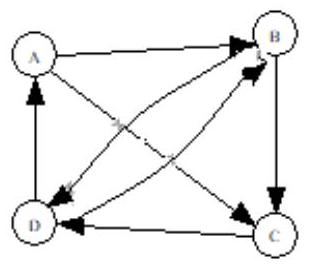
\includegraphics[max width=\textwidth, center]{2025_04_17_46e04c6acd873ea9558dg-231(8)}\\
de lungime 5 ?\\
a) A și B\\
b) A și C\\
c) A și D\\
d) B și C\\
e) $B \operatorname{și} \mathrm{D}$\\
f) C și A\\
10. Fie funcția recursivă de mai jos. Ce valoare va avea apelul $f(f(f(f(0))))$ ?

\begin{verbatim}
Limbajul C++/C
int f(int x)
{if(x<7) return f(x+2)+1;
        else return x-5;}
\end{verbatim}

\begin{verbatim}
Limbajul Pascal
function
f(x:integer):integer;
begin
if x<7 then f:=f(x+2)+1
        else f:=x-5;
end;
\end{verbatim}

a) 1\\
b) 2\\
c) 3\\
d) 4\\
e) 5\\
f) 6\\
11. Indicați ce se va afișa în urma executării următoarei secvențe?

\begin{verbatim}
Limbajul C++/C
int a[6][6]={{2,4,1,5,3},
{5,1,4,2,3},{1,2,3,4,5},{5,4
,3,2,1},{4,1,5,3,2}};
int i,j,k=3;
for(int m=0;m<k;++m)
{for(i=4;i>1;--i)
        for(j=0;j<5;++j)
            a[i+1][j]=a[i][j];
    for(j=0;j<5;j++)
            a[2][j]=a[5][j];
}
for(i=0;i<5;++i)
        {for(j=0;j<5;++j)
                cout<<a[i][j]<< " ";
                |printf("%d ",a[i][j]);
            cout<<endl;|printf("\n"); for i:=0 to 4 do
        }
\end{verbatim}

\begin{verbatim}
                                begin
            for j:= 0 to 4 do
                    write (a[i,j],' ');
        writeln
    end;
\end{verbatim}

\begin{center}
\begin{tabular}{llllll}
a) & b) & c) & d) & e) & f) \\
23154 & 24153 & 24153 & 24153 & 24153 & 34152 \\
51423 & 41532 & 51423 & 54321 & 54321 & 41532 \\
12345 & 54321 & 12345 & 41532 & 41532 & 54321 \\
54321 & 12345 & 54321 & 51423 & 51423 & 12345 \\
21534 & 51423 & 41532 & 12345 & 12354 & 31425 \\
\end{tabular}
\end{center}

\begin{enumerate}
  \setcounter{enumi}{11}
  \item Folosind metoda backtracking, se determină în ordine crescătoare, toate numerele de $\mathbf{4}$ cifre distincte, oricare două cifre alăturate neputând fi prime. Primele 7 soluții sunt: 1024, 1026, 1028, 1029, 1034, 1036, 1038, ... Indicați care sunt cele 2 numere generate înaintea soluției 7401?\\
a) 7091\\
b) 7195\\
c) 7196\\
d) 7297\\
e) 7397\\
f) 7916\\
7092\\
7198\\
7198\\
7298\\
7398\\
7918
  \item Secvența gradelor dintr-un graf neorientat este formată din gradele tuturor nodurilor grafului, aranjate în ordine descrescătoare. Indicați care dintre următoarele secvențe nu poate fi secvență a gradelor pentru niciun graf?\\
I: $7,6,5,4,4,3,2,1$\\
II: 6, 6, 6, 6, 3, 3, 2, 2\\
III: 7, 6, 6, 4, 4, 3, 2, 2\\
IV: $8,7,7,6,4,2,1,1$\\
a) I și II\\
b) I și IV\\
c) II și IV\\
d) III și IV\\
e) doar II\\
f) doar IV
  \item Fie următoarele funcții recursive de mai jos. Indicați care este complexitatea timp a celor două funcții?
\end{enumerate}

\begin{verbatim}
Limbajul C++/C
int f1(int n)
{if(n<=1) return 0;
    return 2*f1(n-1);
}
int f2(int n)
{ if(n<=1) return n;
        return f2(n-1)+f2(n-1); function
}
\end{verbatim}

\begin{verbatim}
        *
\end{verbatim}

a) $\mathrm{O}\left(\mathrm{n}^{2}\right)$ pentru amândouă\\
c) $O\left(2^{n}\right)$ pentru f1 și $O(n)$ pentru f2\\
e) $\mathrm{O}\left(3^{\mathrm{n}}\right)$ pentru f 1

\begin{verbatim}
f2(n:integer):integer;
begin
        if n<=1 then f2:=n;
f2:=f2(n-1)+f2(n-1)
end;
b) O(n) pentru f1 și $\mathrm{O}\left(2^{\mathrm{n}}\right)$ pentru f2
d) $\mathrm{O}(\mathrm{n})$ pentru amândouă
Limbajul Pascal
function
f1(n:integer) :integer;
begin
    if n<=1 then
        f1:=0;f1:=2*f1(n-1)
end;
                                    f) O(3') pentru f1 și f2
\end{verbatim}

,\\
$\qquad$\\
$\qquad$\\
$\qquad$\\
15. Indicați care este complexitatea următoarei secvențe de instrucțiuni:

\begin{verbatim}
Limbajul C++/C
int n,k,p;
cin>>n>>k;|scanf("%d%d
",&n,&k);
p=1;
while(k>0)
\end{verbatim}

\begin{verbatim}
Limbajul Pascal
var n,k,p:integer;
readln(n,k);
p:=1;
while k>0 do
\end{verbatim}

\begin{verbatim}
if(k%2) p*=n, k--;
else n*=n, k/=2;
\end{verbatim}

a) $\mathrm{O}\left(\log _{2} k\right)$\\
b) $\mathrm{O}\left(\log _{2} n\right)$\\
c) $\mathrm{O}(\mathrm{k})$\\
d) $\mathrm{O}(\mathrm{n})$\\
e) $\mathrm{O}\left(\mathrm{n}^{2}\right)$\\
f) $\mathrm{O}\left(\mathrm{k}^{2}\right)$\\
if $k \bmod 2<>0$ then\\
begin $\mathrm{p}:=\mathrm{p} *_{\mathrm{n}}$; $\operatorname{dec}(\mathrm{k})$\\
end\\
else\\
begin $\mathrm{n}:=\mathrm{n} * \mathrm{n}$; $\mathrm{k}:=\mathrm{k}$ div 2 end;

\section*{Varianta 44}
\begin{enumerate}
  \item Variabila v reține un număr întreg. Indicați ce valoare va avea v după executarea următoarei secvențe de instrucțiuni?
\end{enumerate}

\begin{verbatim}
Limbajul C++/C
v=2;
v=5*v-v%3;
v=v+v/3;
\end{verbatim}

Limbajul Pascal\\
v :=2;\\
$\mathrm{v}:=5 * v-\mathrm{v} \bmod 3 ;$\\
v:=v+v div 3;\\
a) 7\\
b) 8\\
c) 10\\
d) 11\\
e) 12\\
f) 16\\
2. Variabilele $\mathbf{x}$ și $\mathbf{y}$ sunt reale, iar $\mathbf{i}$ și $\mathbf{j}$ sunt întregi. Indicați ce valoare va avea $\mathbf{x}$ după executarea următoarei secvențe de instrucțiuni?

$$
\begin{aligned}
& \text { Limbajul C++/C } \\
& x=1.5 ; y=2.0 ; \\
& i=2 ; j=4 ; \\
& x=x * y+(f l o a t) i / j ;
\end{aligned}
$$

a) 2.15\\
b) 2.5\\
c) 3.0\\
d) 3.15\\
e) 3.5\\
f) 4.0\\
d) 3.15\\

\includegraphics[max width=\textwidth, center]{2025_04_17_46e04c6acd873ea9558dg-235(1)}\\
3. Variabilele i și j sunt întregi. Indicați ce se va afișa după executarea următoarei secvențe?

\begin{verbatim}
Limbajul C++/C
i=2; j=3;
if(j) j--;
    else if(i) i++;
        else j++;
if(!j) i--;
    else if(i) j++;
        else j=0;
cout<<i+j;|printf("%d",i+
j);
\end{verbatim}

a) 0\\
b) 1\\
c) 2\\
d) 3\\
e) 4\\
f) 5

\begin{verbatim}
Limbajul Pascal
i:=2; j:=3;
if j<>0 then dec(j)
    else if i<>0 then
            inc(i)
        else inc(j);
if not(j<>0) then inc(i)
        else if(i<>0) then
                inc(j)
            else j:=0;
\end{verbatim}

write (i+j);\\
4. Indicați ce se va afișa după executarea următoarei secvențe de program?

\begin{verbatim}
Limbajul C++/C
int main()
{
char s[11]="ABCDE",aux[11];
strcat(s+2,"ABCDE");
strcpy(aux, s+3);
strcpy(s,aux);
cout<<s[0]-s[2];
|printf("%d",s[0]-s[2]);
    return 0;}
\end{verbatim}

\begin{verbatim}
Limbajul Pascal
x:=1.5; y:=2.0;
i:=2; j:=4;
x:=x*y+i/j;
\end{verbatim}

\begin{verbatim}
        *
\end{verbatim}


\includegraphics[max width=\textwidth, center]{2025_04_17_46e04c6acd873ea9558dg-235}\\
a) 0\\
b) 1\\
c) 2\\
d) 3\\
e) 4\\
f) 5\\
5. Indicați ce se va afișa după executarea următoarei secvențe de program?

\begin{verbatim}
Limbajul C++
typedef struct
        { int S;}S;
int f(S &s)
{return -- s.S;}
int main()
{ int i;
        S S={2};
    i=f(S);
    cout<<i;
    return 0;
\end{verbatim}

\begin{verbatim}
Limbajul C
typedef struct
{ int S;}S;
int f(S *s)
{
return --(*s).S;}
int main()
{ int i;
    S S={2};
    i=f(&S);
    printf("%d",i);
    return 0;
}
\end{verbatim}

\begin{verbatim}
Limbajul Pascal
type ST=record
S:integer end;
var S:ST=(S:2);
        i:integer;
function f(var
    s:ST) :integer;
begin
dec(s.S);f:=s.S
end;
begin
    i:=f(S) ;write(i)
end.
\end{verbatim}

a) 0\\
b) 1\\
c) 2\\
d) 3\\
e) 4\\
f) eroare de compilare\\
6. Indicați cu ce instrucțiune trebuie înlocuite punctele de suspensie din următoarea secvență, astfel încât aceasta să afișeze numărul de divizori pozitivi ai lui n (număr natural nenul)?

\begin{verbatim}
Limbajul C++/C
int p=1,d,e;
for(d=2;d*d<=n;++d)
{
        for(e=1;n%d==0;e++)
    n/=d;
        p*=e;
}
if(n>1) .....
cout<<p;|printf("%d",p);
\end{verbatim}

\begin{verbatim}
Limbajul Pascal
var p,d,e:integer;
p:=1; d:=2;
while d*d<=n do
    begin
        e:=1;
                while n mod d=0 do
                    begin
                        n:=n div d;
                        inc(e)
                    end;
            p:=p*e
    end;
if n>1 then ...
write(p);
\end{verbatim}

\begin{center}
\begin{tabular}{|l|l|l|}
\hline
a) & b) & c) \\
\hline
Limbajul C++/C & Limbajul C++/C & Limbajul C++/C \\
\hline
$\mathrm{p}^{*}=2$; & $\mathrm{p}^{*}=\mathrm{d}$; & p*=d+1; \\
\hline
\begin{tabular}{l}
Limbajul Pascal \\
p:=p*2; \\
\end{tabular} & \begin{tabular}{l}
Limbajul Pascal \\
p:=p*d; \\
\end{tabular} & LimbajulPascal p:=p*(d+1); \\
\hline
d)Limbajul C++/C & e)Limbajul C++/C & f)Limbajul C++/C \\
\hline
\end{tabular}
\end{center}

\begin{center}
\begin{tabular}{lll}
p*=e; & $\mathrm{p}^{*}=(\mathrm{e}+1) ;$ & $\mathrm{p}^{*}=(\mathrm{d}+1) ;$ \\
Limbajul Pascal & LimbajulPascal & LimbajulPascal $\mathrm{p}:=\mathrm{p}^{*}(\mathrm{~d}+1)$; \\
$\mathrm{p}:=\mathrm{p}^{*} \mathrm{e} ;$ & $\mathrm{p}:=\mathrm{p}^{*}(\mathrm{e}+1) ;$ &  \\
\end{tabular}
\end{center}

\begin{enumerate}
  \setcounter{enumi}{6}
  \item Următoarea secvență afișează numărul de perechi de elemente din vectorul v, cu proprietatea că suma celor două elemente din pereche este divizibilă cu $\mathbf{k} \quad(\mathbf{k}<100)$. Se numără numai perechile (v[i];v[j]) cu proprietatea enunțată care au $\mathbf{i}<\mathbf{j}$, unde i și $\mathbf{j}$ sunt numere naturale, $\mathbf{i}<\mathrm{n}, \mathrm{j}<\mathrm{n}$. Indicați cu ce expresie trebuie înlocuite punctele de suspensie?
\end{enumerate}

\begin{verbatim}
Limbajul C++/C
int v[100],n,k;
cin>>n>>k;
        |scanf("%d%d",&n,&k);
for(int i = 0; i<n; ++i)
cin>>v[i];|scanf("%d",&v
[i]);
int x[100]={0};
for (int i=0; i<n;i++)
    ++x[v[i]%k];
int sum = x[0]*(x[0]-
1)/2;
for(int i=1; i<=k/2 &&
    i!=(k-i); i++)
        sum += x[i] * x[k-i];
if (k % 2 == O) sum +=...;
cout<<sum;
        |printf("%d",sum);
\end{verbatim}

a) $\mathrm{x}[\mathrm{k}]$\\
c) $\mathrm{x}[\mathrm{k}] * \mathrm{x}[\mathrm{k}]$\\
c) $x[k]^{*} x[k]$\\
Limbajul Pascal $\mathrm{x}[\mathrm{k}]^{*}(\mathrm{x}[\mathrm{k}]-1)$ div 2\\
e)\\
f) $x[n] * x[n]$

Limbajul C++/C x[k/2]*(x[k/2]-1)/2\\
Limbajul Pascal $x[k \operatorname{div} 2]^{*}$ ( $x[k \operatorname{div} 2]-1$ ) div 2

\begin{verbatim}
Limbajul Pascal
var n,k,i,sum:integer;
v,x:array[0..99] of integer;
begin
    readln(n,k);
    for i:=0 to n-1 do
        readln(v[i]);
    for i:=0 to n-1 do
            inc(x[v[i] mod k]);
    sum:=x[0]*(x[0]-1)div 2;
    i:=1;
    while (i<=k div 2) and
        (i<>(k-i)) do
        begin
            sum:=sum+x[i]*x[k-i];
            inc(i)
        end;
    if k mod 2=0 then
        sum:=sum+...;
        write(sum);
end.
\end{verbatim}

b) $x[n]$

\section*{d)}
Limbajul C++/C x[k]*(x[k]-1)/2\\
$\qquad$

\begin{verbatim}
2
``` 2
8. Variabilele i şi j sunt de tip întreg, iar variabila a memorează un tablou bidimensional cu n linii şi n coloane, numerotate de la 0 la $\mathbf{n - 1}$, având iniţial toate elementele egale
cu -1. Matricea se împarte în 4 cadrane astfel:
![](https://cdn.mathpix.com/cropped/2025_04_17_46e04c6acd873ea9558dg-238.jpg?height=142&width=171&top_left_y=355&top_left_x=1210)

Indicați cu ce instrucțiune trebuie înlocuite punctele de suspensie astfel încât, în urma executării secvenței obținute, tabloul a să memoreze în cadranul I, doar valoarea 1, în cadranul II, doar valoarea 2, în cadranul III doar valoarea 3 iar în ultimul cadran doar valoarea 4.
\end{verbatim}

LimbajC++/C\\
for (i=0; $i<n / 2 ; i++$ )\\
for ( $j=i+1$; $j<n-i-1$;\\
j++)\\
\{\\[0pt]
a[i][j]=1;\\
...;\\[0pt]
a[n-i-1][j]=3;\\[0pt]
a[j][i]=4;\\
)\\
a)

\begin{verbatim}
Limbajul C++/C a[i][n-j]=2;
Limbajul Pascal $a[i, n-j]:=2 ;$
c)
\end{verbatim}

Limbajul C++/C a[n-j-1][n-i-1]=2;\\[0pt]
Limbajul Pascal a[n-j-1,n-i-1]:=2;\\
e)\\[0pt]
Limbajul C++/C a[j][n-i]=2; Limbajul C++/C a[i][i]=2;\\[0pt]
Limbajul Pascal a[j][n-i]:=2;

\begin{verbatim}

\end{verbatim}

Limbaj Pascal\\
for $i:=0$ to $n$ div 2-1 do\\
for $j:=i+1$ to $n-i-2$ do\\
begin\\[0pt]
a[i,j]:=1;\\
...;\\
$a[n-i-1, j]:=3$;\\[0pt]
a[j,i]:=4\\
end;\\
b)

\begin{verbatim}

\end{verbatim}

Limbajul C++/C a[n-i][n-j]=2; Limbajul Pascal a[n-i,n-j]:=2;

\begin{verbatim}

\end{verbatim}

d)\\[0pt]
Limbajul C++/C a[n-j][n-i]=2; Limbajul Pascal a[n-j,n-i]:=2; f)\\
$\begin{array}{ll}\text { Limbajul } \mathbf{C +}+/ C & a[i][i]=2 ; \\ \text { Limbajul Pascal } & a[i][i]:=2 ;\end{array}$

\begin{verbatim}
9. Fie funcția recursivă de mai jos. Indivați ce valoare va avea apelul $f(16)$ ?
\end{verbatim}

Limbajul C++/C\\
int f(int x)\\
\{if(x>8)\\
return f(f(x-3))+4;\\
else return x-5;\\
\}

\begin{verbatim}
a) -5
b) -2
c) -1
\end{verbatim}

Limbajul Pascal\\
function f(x:integer):integer;\\
begin\\
if x>8 then\\
f:=f(f(x-3))+4\\
else f:=x-5;\\
end;

\begin{verbatim}
d) 1
e) 2
f) 5
10. Indicați câte componente tare conexe are graful orientat $\mathrm{G}=(\mathrm{V}, \mathrm{E})$ unde $\mathrm{V}=\{\mathbf{1}, \mathbf{2}, \mathbf{3}$, $4,5,6,7,8,9,10\}$ iar $E=\{(1,2),(1,7),(1,10),(2,6)$, $(3,2),(3,5),(3,9),(4,3),(4,6),(5,2),(6,1),(8,7)$, $(9,6),(9,8)\} ?$
a) 6
b) 7
c) 8
d) 9
e) 10
f) 5
11. Folosind metoda backtracking, se determină în ordine lexicografică, toate cuvintele de 6 litere distincte din mulțimea $\{\mathbf{a}, \mathbf{e}, \mathrm{i}, \mathrm{o}, \mathbf{u}, \mathbf{b}, \mathbf{c}, \mathrm{d}, \mathrm{m}, \mathrm{n}, \mathrm{p}\}$, oricare două litere alăturate neputând fi vocale. Primele 5 soluții sunt: abecid, abecim, abecin, abecip, abecod. Indicați care cuvânt este generat înaintea soluției ebacid?
a) mnpdb
b) apcdmn
c) apmncd
d) apmndc
e) apnmdc
f) ebdcpa
12. Fie un graf neorientat G cu 1002 noduri numerotate cu numere naturale consecutive de la 1 la 1002. Știind că oricare două noduri de aceeași paritate sunt adiacente, se cere să indicați cum trebuie modificat graful, astfel încât acesta să devină eulerian.
a) se elimină două muchii
b) se elimină o muchie și se
c) se adaugă două muchii adaugă două muchii noi noi
d) se elimină o muchie
e) se adaugă trei muchii noi
f) se elimină trei muchii
13. Fie un arbore cu rădăcină care are 5000 de noduri iar fiecare nod are maxim 4 fii. Indicați care este înălțimea minimă a arborelui?
a) 4
b) 5
c) 6
d) 7
e) 8
f) 9
14. Indicați care este complexitatea următoarei funcții?
\end{verbatim}

Limbajul C++/C\\
void f(int n)\\
\{int i ,j,nr=0;\\
for(i=n/2; i<=n; i++)\\
for(j=n; j>=1; j/=2)\\
nr++;\\
\}

\begin{verbatim}

Limbajul Pascal
\end{verbatim}

procedure f(n:integer);\\
var i,j,nr:integer;\\
begin\\
for i:=n div 2 to n do\\
begin\\
j:=n;\\
while j>=1 do\\
begin\\
inc(nr);\\
j:=j div 2\\
end\\
end\\
end;

\begin{verbatim}
a) $\mathrm{O}(\log n)$
b) $O\left(n^{2}\right)$
c) $\mathrm{O}\left(\mathrm{n}^{2} \operatorname{logn}\right)$
d) $\mathrm{O}(\mathrm{nlogn})$
e) $O(n)$
f) $\mathrm{O}\left(\mathrm{n}^{3}\right)$
15. Fie $\mathbf{x}, \mathbf{a}_{0}, \mathbf{a}_{1}, \ldots, \mathbf{a}_{\mathbf{n}}$ numere reale nenule. Indicați numărul minim de înmulțiri care este necesar pentru a calcula optim $a_{0}+a_{1} * \mathbf{x}+a_{2} * \mathbf{x}^{2}+a_{3} * \mathbf{x}^{3}+\ldots+a_{n} * \mathbf{x}^{n}$ ?
a) $n-1$
b) $n$
c) $\frac{n}{2}$
d) $\frac{(n+1)(n+2)}{2}$
e) $\mathrm{n}-2$
f) $\frac{(n-1)(n+1)}{2}$

\section*{Varianta 45}
1. Variabilele întregi i, $\mathbf{j}, \mathbf{k}$ memorează numere naturale. Valoarea variabilei $\mathbf{k}$ după rularea următoarei secvențe de instrucțiuni este?
$$
\begin{array}{r}
\text { Limbajul C/C++ } \\
i=4 ; \quad j=5 ; \quad k=--i * j++;
\end{array}
$$
$$
\begin{aligned}
& \quad \text { Limbajul Pascal } \\
& i:=4 ; j:=5 ; \operatorname{dec}(i) ; \\
& k:=\mathrm{i} * j ; i n c(j) ;
\end{aligned}
$$
a) 12
b) 13
c) 14
d) 15
e) 16
f) 17
2. Variabilele întregi i, j, k memorează numere naturale. Valoarea variabilei k, după rularea următoarei secvențe de instrucțiuni, este?
$$
\begin{aligned}
& \quad \text { Limbajul C/C++ } \\
& i=3 ; \quad j=-3 ; k=i * j ; \\
& k+=j ; \quad k /=i ;
\end{aligned}
$$

\section*{Limbajul Pascal} i:=3; j:=-3; k:=i*j; k:=k+j; k:=k div i;
a) -8
b) -6
c) -4
d) 4
e) 6
f) 8
3. Variabilele întregi i, j, k memorează numere naturale. După rularea următoarei secvențe de instrucțiuni se va afișa?
\end{verbatim}

Limbajul C/C++

\begin{verbatim}

\end{verbatim}

i=2; j=-2; if(j) i--;\\
if(i) j++; k=i*j;\\
cout<<k;|printf("\%d",k);

\begin{verbatim}

\section*{Limbajul Pascal}
\end{verbatim}

i:=2; j:=-2;\\
if j<>0 then dec(i);\\
if(i<>0) then inc(j); k:=i*j;\\
write(k);

\begin{verbatim}
a) -2
b) -1
c) 0
d) 1
e) 2
f) 3
4. După rularea următorului program se afișează?
\end{verbatim}

Limbajul C++\\
\#include<iostream>\\
using namespace std;\\
int f(int\&i)\\
\{ return i++;\\
\}\\
int main()\{\\
int i=1,j;\\
j=f(i);\\
cout<<i<<' '<<<j;\\
return 0;\\
\}

\begin{verbatim}

\end{verbatim}

int f(int *i)\\
\{\\
return (*i)++;\\
\}\\
int main() \{\\
int i=1,j;\\
j=f(\&i);\\
printf("\%d \%d",i,j);\\
return 0;\\
\}

\begin{verbatim}

\section*{Limbajul C}
\#include <stdio.h>

\section*{Limbajul Pascal}
\end{verbatim}

var i,j:integer;\\
function f(var\\
i:integer):integer;\\
begin\\
f:= i; inc(i)\\
end;\\
begin\\
i:=1; j:=f(i);\\
write(i,' ',j)\\
end.

\begin{verbatim}
a) 02
b) 11
c) 12
d) 21
e) 22
f) eroare de compilare
5. După rularea programului de mai jos se afișează?
\end{verbatim}

Limbajul C++\\
\#include<iostream>\\
using namespace std;\\
struct S\\[0pt]
\{int a[2];\};\\
int main()\\
\{\\[0pt]
S S[2]; int i;\\
for(i=0;i<2;i++)\\[0pt]
S[i].a[1-i]=4*!i;\\[0pt]
cout<<S[0].a[1];\\
return 0;\\
\}

\begin{verbatim}

\end{verbatim}

Limbajul C\\
\#include <stdio.h>\\
struct S\\[0pt]
\{int a[2];\};\\
int main() \{\\[0pt]
struct S S[2];\\
int i;\\
for(i=0;i<2;i++)\\[0pt]
S[i].a[1-i]=4*!i;\\
printf("\%d",\\[0pt]
S[0].a[1]);\\
return 0;\}

\begin{verbatim}

\end{verbatim}

Limbajul Pascal\\
type ST=record\\[0pt]
a:array[0..1] of\\
integer\\
end;\\[0pt]
var S:array[0..1] of\\
ST;\\
i:integer;\\
begin\\
for i:=0 to 1 do\\[0pt]
S[i].a[1-i]:=\\
4*(1-i);\\[0pt]
write(S[0].a[1])\\
end.

\begin{verbatim}
a) 0
b) 1
c) 2
d) 3
e) 4
f) 5
6. Variabilele întregi $\mathbf{i}, \mathbf{x}$ memorează numere naturale. Numărul de numere afișate după executarea următoarei secvențe de instrucțiuni este?
\end{verbatim}

\begin{verbatim}
        Limbajul C/C++
\end{verbatim}

for(i=1;i<=10000;i++)\\
\{x=i-4;\\
while(x>2\\
\&\&(x\%10\hl{0 | | x\%10}2))\\
x=x/10, x=x-4;\\
if(x\hl{0 || x}2)\\
cout<<i;|printf("\%d",i);\\
\}

\begin{verbatim}

\section*{Limbajul Pascal}
\end{verbatim}

for i:=1 to 10000 do begin\\
x:=i-4;\\
while (x>2) and ((x mod\\
10=0) or (x mod 10=2)) do\\
begin\\
x:=x div 10; x:=x-4\\
end;\\
if (x=0) or (x=2) then\\
write(i)\\
end;

\begin{verbatim}
a) 100
b) 50
c) 45
d) 40
e) 35
f) 30
7. Tabloul bidimensional a , pătratic, are liniile și coloanele numerotate de la 1 la 1000 și
este împărțit în 4 zone delimitate de diagonale, ca în desen
![](https://cdn.mathpix.com/cropped/2025_04_17_46e04c6acd873ea9558dg-241.jpg?height=145&width=177&top_left_y=1868&top_left_x=1375) Variabilele întregi i, j, s memorează numere naturale. Elementele care sunt adunate în algoritmul următor se găsesc în zona/zonele?
\end{verbatim}

\begin{verbatim}
        Limbajul C/C++
\end{verbatim}

s=0;\\
for(i=120;i<=380;++i)\\
for(j=i+1;j<=1000-i;j++)\\[0pt]
s+=a[1001-j][1001-i];

\begin{verbatim}

\end{verbatim}

s:=0;\\
for i:=120 to 380 do\\
for j:=i+1 to 1000-i\\
do\\[0pt]
s:=s+a[1001-j,1001-i];

\begin{verbatim}

Limbajul Pascal
a) I
b) I și II
c) II
d) II și III
e) II și IV
d) IV
8. După rularea următoarei secvențe de instrucțiuni se afișează?
\end{verbatim}

\begin{verbatim}
Limbajul C/C++
\end{verbatim}

char s[100]="UPB-\\
automatica",*p;\\
p=strchr(s,'-');\\[0pt]
(p+1)[0]-=32; s[p-s]='\textbackslash 0';\\
p++; strcat(p,"-");\\
strcat(p,s); strcpy(s,p);\\
cout<<s;|printf("\%s",s);

\begin{verbatim}
a) Auto
b) Automatica-UPB
c) Auto-UPB
d) UPB
e) automatica-UPB
f) automatica-UPB-automatica
9. Pentru ca tabloul unidimensional a să fie ordonat crescător după rularea secvenței de instrucțiuni de mai jos, punctele de suspensie se înlocuiesc cu?
\end{verbatim}

Limbajul C/C++\\[0pt]
int a[10]=\{8, 2, 1, 9,\\
10, 3, 7, 5, 4, 6\},\\[0pt]
b[10]=\{ 0 \}, c[10],i, j;\\
for(i=0;i<10;++i)\\
for(j=i+1;j<10;++j)\\
if(...)\\[0pt]
b[i]++;\\[0pt]
else b[j]++;\\
for(i=0;i<10;i++)\\[0pt]
c[b[i]]=a[i];\\
for(i=0;i<10;i++)\\[0pt]
a[i]=c[i];

\begin{verbatim}
a) a[i]<a[j]
c) $a[i]!=a[j] \mid a[i]<>a[j]$
e) $a[i]+a[j]$

\section*{Limbajul Pascal}
\end{verbatim}

var a:array[0..9] of integer=\\
(8,2,1,9,10,3,7,5,4,6);\\[0pt]
b, c:array[0..9] of integer;\\
i, j:integer;\\
for i:=0 to 9 do\\
for j:=i+1 to 9 do\\[0pt]
if ..... then inc(b[i])\\[0pt]
else inc(b[j]);\\
for i:=0 to 9 do\\[0pt]
c[b[i]]:=a[i];\\[0pt]
for i:=0 to 9 do a[i]:=c[i];

\begin{verbatim}
b) $a[i]<=a[j]$
d) $a[i]==a[j] \mid a[i]=a[j]$
f) $a[i]>a[j]$
                b) $a[i]<=a[j]$
            $a[i]==a[j] \mid a[i]=a[j]$
            f) $a[i]>a[j]$
10. Apelul $f(19,7)$ are valoarea?
\end{verbatim}

Limbajul C/C++\\
int f(int x, int y)\\
\{\\
if(x>y)

\begin{verbatim}

\section*{Limbajul Pascal}
\end{verbatim}

var s,p:string; i:integer;\\
s:='UPB-automatica'; i:=pos('-\\
',s);\\[0pt]
s[i+1]:=chr(ord(s[i+1])-32);\\
p:=copy(s,i+1,length(s)-i);\\
delete(s,i,length(s)-i+1);\\
s:=p+'-'+s;\\
write(s);

\begin{verbatim}

\end{verbatim}

\begin{verbatim}
            Limbajul Pascal
\end{verbatim}

function f(x,y:integer):integer;\\
begin\\
if x>y then f:=f(x-3,y+1)-2\\
else if \}x=y\textbackslash mathrm\{ then

\begin{verbatim}

\end{verbatim}

Limbajul C/C++\\[0pt]
void f(int n, int v[101])\\
\{\\
int i, j=0;\\
for(i=0;i<n;i++)\\[0pt]
while(j<n \&\& v[i]<v[j])\\
j++;\\
\}

\begin{verbatim}
a)$O(\sqrt{n})$
b)$O(n)$
\end{verbatim}

\begin{verbatim}
return f(x-3, y+1)-
\end{verbatim}

2;\\
else\\
if(x==y)\\
return f(x+1, y);\\
else\\
return 3\textit{x-\\
2}y;\}

\begin{verbatim}

\end{verbatim}

\textbackslash 

\begin{verbatim}
a)-6
b)-5
c) $\mathbf{- 4}$
d) 4
都
d) 4

11.Folosind metoda backtracking,se determină în ordine descrescătoare,toate numerele de 4 cifre nenule distincte,cifrele impare apar în ordine descrescătoare,cele pare în ordine crescătoare și oricare două cifre alăturate nu pot fi pare,.Primele 7 soluții sunt:9875, 9873,9871,9853,9851,9831.Cele 3 numere generate înaintea soluției 3416 sunt?
a) 361834213418
c) 431636183418
d) $43184316 \quad 3618$
e) 451643183418![](https://cdn.mathpix.com/cropped/2025_04_17_46e04c6acd873ea9558dg-243.jpg?height=66&width=31&top_left_y=1048&top_left_x=788)

f) 451245164518

12.Fie $\mathbf{T}$ un arbore oarecare cu un număr par de noduri,în care fiecare nod are maxim 2 fii. Numărul maxim de noduri de pe ultimul nivel i,știind că rădăcina arborelui se află pe nivelul 1,este?
a) $2^{\text {i+1 }}$
b) $2^{i}+1$
c) $\mathbf{2}^{\text {i }}$
d) $2^{\frac{i+1}{2}}$
e) $2^{\mathrm{i}-1}$
f) $2^{\mathrm{i}-1}-1$
 astfel încât fiecare muchie are o extremitate în prima submulțime și cealaltă în a doua submulțime.Fie G un graf neorientat,bipartit,cu 10 noduri.Numărul maxim de muchii pe care poate să le aibă graful $G$ este?
a) 5
b) 15
c) 25
d) 35
f) 55
b) 15d) 35

14.Complexitatea următoarei funcții este?
\end{verbatim}

end;

\begin{verbatim}

\end{verbatim}

f:=f(x+1,y)\\
else f:=3\textit{x-2}y

\begin{verbatim}

\end{verbatim}

\begin{verbatim}
lse f:=3*x-2*y
\end{verbatim}

\begin{verbatim}
![](https://cdn.mathpix.com/cropped/2025_04_17_46e04c6acd873ea9558dg-243.jpg?height=47&width=101&top_left_y=341&top_left_x=1344)
                                                    
\end{verbatim}

\begin{itemize}
  \item 
\end{itemize}

\begin{verbatim}

\section*{5}
c)-4
e) 5
f) 6
f) 6
e) 5
f) 6 crescătoare și oricare două cifre alăturate nu pot fi pare,.Primele 7 soluții sunt:9875,9873,9871,9853,9851,9831.Cele 3 numere generate înaintea soluției 3416

b) 381643124316le de 4
                    
$\qquad$
                                                                                                    2
                                                                                        ii![](https://cdn.mathpix.com/cropped/2025_04_17_46e04c6acd873ea9558dg-243.jpg?height=83&width=55&top_left_y=1677&top_left_x=1810)
![](https://cdn.mathpix.com/cropped/2025_04_17_46e04c6acd873ea9558dg-243.jpg?height=28&width=12&top_left_y=1878&top_left_x=1805)

![](https://cdn.mathpix.com/cropped/2025_04_17_46e04c6acd873ea9558dg-243.jpg?height=28&width=12&top_left_y=1878&top_left_x=1805)![](https://cdn.mathpix.com/cropped/2025_04_17_46e04c6acd873ea9558dg-243.jpg?height=50&width=61&top_left_y=1856&top_left_x=1799)
-_
-

    .
-
-
$\square$

![](https://cdn.mathpix.com/cropped/2025_04_17_46e04c6acd873ea9558dg-243.jpg?height=47&width=131&top_left_y=1534&top_left_x=1965)
都
c) 25
\begin{tabular}{|l|l|}
\hline mitate în prima submulțime și cealaltă în a dou bipartit,cu 10 noduri.Numărul maxim de mu & \\
\hline
\end{tabular}

13.Un graf este bipartit dacă nodurile lui pot fi împărțite în două submulțimi disjuncte,
13.Un graf este bipartit dacă nodurile lui pot fi împățite în două submulțimi disju

e) 45
$\begin{array}{ll}\text { e)} \mathbf{4 5} & \text { f)} 55\end{array}$
 
,

            nivelul 1,este?
a) $2^{i+1}$
b) $2^{i}+1$
c) $2^{1}$
d) $2^{2}$都正
.
- ..... 
fii.

    
![](https://cdn.mathpix.com/cropped/2025_04_17_46e04c6acd873ea9558dg-243.jpg?height=23&width=26&top_left_y=1338&top_left_x=1902) ![](https://cdn.mathpix.com/cropped/2025_04_17_46e04c6acd873ea9558dg-243.jpg?height=23&width=22&top_left_y=1341&top_left_x=1908)![](https://cdn.mathpix.com/cropped/2025_04_17_46e04c6acd873ea9558dg-243.jpg?height=60&width=28&top_left_y=634&top_left_x=1932)ou
-
![](https://cdn.mathpix.com/cropped/2025_04_17_46e04c6acd873ea9558dg-243.jpg?height=18&width=20&top_left_y=1799&top_left_x=1775)
![](https://cdn.mathpix.com/cropped/2025_04_17_46e04c6acd873ea9558dg-243.jpg?height=134&width=44&top_left_y=1417&top_left_x=1794)

![](https://cdn.mathpix.com/cropped/2025_04_17_46e04c6acd873ea9558dg-243.jpg?height=20&width=25&top_left_y=1035&top_left_x=2076)

![](https://cdn.mathpix.com/cropped/2025_04_17_46e04c6acd873ea9558dg-243.jpg?height=31&width=28&top_left_y=1081&top_left_x=2046)
procedure $f(\mathrm{n}$ :integer;

        v:array[0..100] of

integer) ;

var i,j:integer;

begin

j: =0;

for i:=0 to n-1 do

    while (j<n) and (v[i]<v[j]) do

inc(j)

end;


d) $O\left(n^{2}\right)$
e) $O\left(n(\log n)^{2}\right)$
f) $O\left(n^{3}\right)$

15

Numărul de drumuri de lungime 3 din graful orientat alăturat este?
a) 10
b) 15
c) 20
d) 25
e) 30
f) 40

\section*{Varianta 46}
1. Variabila întreagă v memorează numere naturale. Valoarea variabilei v după rularea următoarei secvențe de instrucțiuni este?
\end{verbatim}

Limbajul C/C++\\
v=2; v=v\textit{v; v=v-v\%2}3;\\
v=v\%3+5;

\begin{verbatim}
a) 4
b) 5
c) 6
d) 7
e) 8
f) 9
4

\section*{5}
2. Variabilele întregi i, $\mathbf{x}$ memorează numere naturale. Numărul de numere de 5 cifre ce vor fi afișate după rularea următoarei secvențe de instrucțiuni este?
\end{verbatim}

\begin{verbatim}
    Limbajul C/C++
\end{verbatim}

for(i=1;i<=100000;i++) \{\\
x=i-5;\\
while(x>2\&\&(x\%10\hl{0 | |x\%10}2))\\
x=x/10,x=x-5;\\
if(x\hl{0 || x}2)\\
cout<<i;\\
|printf("\%d",i);\\
\}

\begin{verbatim}
a) $\mathbf{2 8}$
b) 29
c) 30
d) 31
e) 32
f) 33
.
3. După rularea următoarei secvențe de instrucțiuni se afișează?
\end{verbatim}

\begin{verbatim}
                Limbajul C/C++
\end{verbatim}

int i=0,j=5,aux,\\[0pt]
v[]=\{41,52,26,11,48,65\};\\
while(i<j)\{\\[0pt]
for(;i<j \&\& !(v[i]\%2);i++);\\[0pt]
for(;i<j \&\& (v[j]\%2);j--);\\
if(i<j)\\[0pt]
aux=v[i],v[i]=v[j],v[j]=aux;\\
\}\\
for(i=0;i<6;++i)\\[0pt]
cout<<v[i]<<" ";|\\[0pt]
printf("\%d ",v[i]);

\begin{verbatim}

\end{verbatim}

for i:=1 to 100000 do\\
begin\\
x:=i-5;\\
while (x>2) and((x mod\\
10=0) or (x mod 10=2)) do\\
begin\\
x:=x div 10; x:=x-5\\
end;\\
if (x=0) or (x=2) then\\
write(i)\\
end;\\
*

\begin{verbatim}
$\mathrm{v}:=2 ; \mathrm{v}:=\mathrm{v} * \mathrm{v} ;$
$\mathrm{v}:=\mathrm{v}-\mathrm{v} \bmod 2 * 3 ;$
$\mathrm{v}:=\mathrm{v} \bmod 3+5 ;$

\section*{Limbajul Pascal}

\section*{6}

\section*{Limbajul Pascal}
\end{verbatim}

Limbajul Pascal\\
var i,j,aux:integer;\\[0pt]
v:array[0..5] of\\
integer= (41, 52, 26,11,\\
48, 65);\\
i:=0; j:=5;\\
while i<j do begin\\[0pt]
while (i<j) and (not(v[i]\\
mod 2=1)) do\\
inc(i);\\[0pt]
while (i<j) and(v[j] mod\\
2=1) do dec(j);\\
if i<j then begin\\[0pt]
aux:=v[i];\\[0pt]
v[i]:=v[j];\\[0pt]
v[j]:=aux end;\\
end;

\begin{verbatim}

\end{verbatim}

for i:=0 to 5 do\\[0pt]
write(v[i],' ');

\begin{verbatim}
a) $11 \quad 26 \quad 41 \quad 48 \quad 52 \quad 65$
b) $65 \quad 41 \quad 11 \quad 52 \quad 48 \quad 26$
c) $26 \quad 48 \quad 52 \quad 11 \quad 41 \quad 65$
d) $48 \quad 52 \quad 26 \quad 11 \quad 41 \quad 65$
e) $5248 \quad 26 \quad 65 \quad 41 \quad 11$
f) $11 \quad 41 \quad 65 \quad 48 \quad 52 \quad 26$
4. După rularea următoarei secvențe de instrucțiuni se afișează?
\end{verbatim}

\begin{verbatim}
Limbajul C/C++
\end{verbatim}

char s[50]="test informatica";\\
char *p;\\
strtok(s, " ");\\
p=strtok (NULL," ") ;\\
strcpy(s,strcat(p,s));\\
cout<<s;|printf("\%s",s);

\begin{verbatim}

\section*{Limbajul Pascal}
\end{verbatim}

var s,p:string;\\
s:='test informatica';\\
p:=copy(s,pos(' ' ,s)+1,\\
length(s) - pos(' ',s));\\
delete(s,pos(' ' ,s),\\
length(s)-pos(' ',s)+1);\\
s:=p+s; write(s);

\begin{verbatim}
a) testtest
b) testinformatica
c) test
d) informaticatest
e) informatica
f) info
5. Pentru ca secvența următoare de instrucțiuni să determine dacă cele $\mathbf{n}$ intervale memorate în tabloul unidimensional v sunt disjuncte, punctele de suspensie se înlocuiesc cu?
\end{verbatim}

\begin{verbatim}
        Limbajul C/C++
\end{verbatim}

struct interval\{int x, y;\}\\[0pt]
v[100];\\
int i, j, r, t,n;\\[0pt]
r=v[0].x; t=v[0].Y;\\
for(i=1;i<n;++i) \{\\[0pt]
if(r<v[i].x) r=v[i].x;\\[0pt]
if(t>v[i].y) t=v[i].y;\}\\
if(...)\\
cout<<"DA";|printf("DA");\\
else\\
cout<<"NU";|printf("NU");

\begin{verbatim}

\end{verbatim}

Limbajul Pascal\\
type interval=record\\
x,y:integer end;\\[0pt]
var v:array[0..99] of\\
interval;\\
i,j,r,t,n:integer;\\[0pt]
r:=v[0].x; t:=v[0].y;\\
for i:=1 to n-1 do begin\\[0pt]
if r<v[i].x then\\[0pt]
r:=v[i].x;\\[0pt]
if t>v[i].y then\\[0pt]
t:=v[i].Y\\
end;\\
if ... then write('DA')\\
else write('NU');

\begin{verbatim}
a) $r<t$
b) $r<=t$
c) $r==t$
d) $r!=t \quad r<>t$
e) $r>=t$
f) $r>t$
6. Variabilele întregi i, j, s memorează numere naturale. Tabloul bidimensional a, pătratic, cu elemente numere naturale, are $\mathbf{n}$ linii și $\mathbf{n}$ coloane, numerotate de la 1 la $\mathbf{n}$ și
este împărțit în 4 zone ca în desen
![](https://cdn.mathpix.com/cropped/2025_04_17_46e04c6acd873ea9558dg-247.jpg?height=134&width=172&top_left_y=356&top_left_x=1012) Pentru ca algoritmul următor să adune elemente din zona II, punctele de suspensie se înlocuiesc cu?
\end{verbatim}

Limbajul C++/C\\
s=0;\\
for(i=1;i<=(n-1)/2;++i)\\
for(j=i+1;j<=n-i;j++)\\
s+=.....;

\begin{verbatim}
a) $a[n-i+1][j]$ | $a[n-i+1, j]$
c) $a[n+1-i][n+1-j]$ | $a[n+1-i, n+1-j]$
e) $a[j][i]$ | $a[j, i]$
\end{verbatim}

Limbajul Pascal\\
s:=0;\\
for i:=1 to (n-1) div 2 do\\
for j:=i+1 to n-i do\\
s:=s+.....;

\begin{verbatim}
b) $a[i][j]$ | $a[i, j]$
d) $a[n-i][n-j] \mid a[n-i, n-j]$
f) $a[n+1-j][n+1-i]$ | a[n+1-j, n+1-i]
7. Pentru ca, după rularea următoarei secvențe de instrucțiuni, să se afișeze valoarea 7, punctele de suspensie se înlocuiesc cu?
\end{verbatim}

\begin{verbatim}
                Limbajul C/C++
\end{verbatim}

int i, P, v[10]=\{2, 6, 8, 12,\\
20, 25, 30, 37, 41, 92\};\\
for (p = 1; p < 10; p *=2);\\
for (i = 0; p; ...)\\[0pt]
if (i+p<10 \&\& v[i+p]<= 40)\\
i += p;\\
cout<<i;|printf("\%d",i);

\begin{verbatim}

\section*{Limbajul Pascal}
var v:array[0..9] of integer $=(2,6,8,12$, $20,25,30,37,41, ~ 92)$;
i,p:integer;
p:=1;
while $\mathrm{p}<10$ do $\mathrm{p}:=\mathrm{p} * 2$;
i: =0;
while $\mathrm{p}<>0$ do begin if (i+p<10) and
$(v[i+p]<=40)$ then
i:=i+p;
p:=.......;
end;
write (i) ;
a) $p /=2 \mid p$ div 2
b) $p * 2$
c) $p++\mid p+1$
d) $\mathrm{p}-\mathrm{-} \mid \mathrm{p}-1$
e) $p+2$
f) $p+=i \mid p+i$
8. După rularea următorului program se afișează?
\begin{tabular}{l|c|c}
\multicolumn{1}{c|}{ Limbajul C++ } & Limbajul C & Limbajul Pascal \\
\#include<iostream> & \#include <stdio.h> & type QT = record \\
using namespace & struct Q\{ \\
std; & int $a, b, c ;\} ;$ & $a, b, c:$ integer \\
end;
\end{tabular}
\end{verbatim}

struct Q\{\\
int a, b, c;\};\\
struct S\{\\
int a, b, c;\\
struct Q Q;\};\\
int main()\{\\
Q Q=\{3, 2, 1\};\\
S S=\{4, 5, 6\};\\
S.Q=Q;\\
cout<<<S.b-S.Q.b;\\
return 0;\}

\begin{verbatim}

\end{verbatim}

struct S\{\\
int a, b, c;\\
struct Q Q;\};\\
int main() \{\\
struct Q Q=\{3,2,1\};\\
struct S S=\{4,5,6\};\\
S.Q=Q;\\
printf("\%d", S.b-S.Q.b);\\
return 0;\}

\begin{verbatim}
a) 5
b) 4
c) 3
d) 2
e) 1
f) 0
1
()
0
\end{verbatim}

ST = record\\
a,b,c:integer;\\
Q:QT end;\\
var Q:QT =\\
(a:3;b:2;c:1);\\
S:ST =\\
(a:4;b:5;c:6);\\
begin\\
S.Q:=Q;\\
write(S.b-S.Q.b)\\
end.

\begin{verbatim}
9. Apelul $f(6,2)$ are valoarea?

\section*{Limbajul C/C++}
\end{verbatim}

int f(int x, int y) \{\\
if (x>y)\\
return f(f(y,x), x/y)-1;\\
else\\
if (x==y)\\
return f(x+y, x)+2;\\
else return y-x;\}

\begin{verbatim}

\end{verbatim}

Limbajul Pascal\\
function f(x,y:integer):\\
integer;\\
begin\\
if x>y then\\
f:=f(f(y,x),x div y)-1\\
else if x=y then\\
f:=f(x+y,x)+2\\
else\\
f:=y-x;\\
end;

\begin{verbatim}
a) 0
b) 1
c) 2
d) 3
e) 4
f) 5
10. Numărul de circuite elementare diferite (care au cel puțin un arc diferit) care trec prin
![](https://cdn.mathpix.com/cropped/2025_04_17_46e04c6acd873ea9558dg-248.jpg?height=253&width=329&top_left_y=1684&top_left_x=1082)
nodul A din graful orientat alăturat este?
a) 4
b) 5
c) 6
d) 7
e) 8
f) 9
11. Folosind metoda backtracking, se determină în ordine lexicografică, toate cuvintele de $\mathbf{4}$ litere distincte din mulțimea $\{\mathbf{a}, \mathbf{b}, \mathbf{e}, \mathbf{f}, \mathbf{g}, \mathbf{i}, \mathbf{l}, \mathbf{m}, \mathbf{o}, \mathbf{p}, \mathbf{r}, \mathbf{u}\}$ oricare două litere alăturate să nu fie consecutive în mulțimea dată, iar vocalele să apară în ordine descrescătoare. Primele 5 soluții sunt: $a f b g$, $a f b l$, $a f b m, ~ a f b p, ~ a f b r . ~$ Cele 2 cuvinte generate înaintea cuvântului elaf sunt?
a) farg farl
b) egrl egrm
c) $\operatorname{egmf} \operatorname{egmp}$
d) eglr eglu
e) buri buro
f) bopl bupm
12. Un arbore oarecare cu rădăcină este reprezentat prin vectorul de tați $t$. Dacă algoritmul următor determină nivelul pe care se găsește un nod $\mathbf{x}$ în arbore, cu ce secvență de cod se pot înlocui punctele de suspensie de mai jos?
\end{verbatim}

Limbajul C/C++\\
int nivel=0;\\[0pt]
while(t[x])\{\\
nivel++;\}

\begin{verbatim}
a) $t[\mathbf{x}]=\mathbf{x} ; \quad \mathrm{t}[\mathbf{x}]:=\mathbf{x}$;
b) $\mathrm{t}[\mathrm{x}]-\mathrm{-}$; $\mid \mathrm{t}[\mathrm{x}]:=\mathrm{t}[\mathrm{x}]-1$;
c) $\mathbf{x}=\mathrm{t}[\mathrm{x}]$; $\mid \mathbf{x}:=\mathrm{t}[\mathbf{x}]$;
d) $\mathrm{t}[\mathrm{x}]++$; $\mid \mathrm{t}[\mathrm{x}]:=\mathrm{t}[\mathrm{x}]+1$;
e) $x=t[t[x]] ; \quad \mid x:=t[t[x]]$;
f) $\mathrm{t}[\mathrm{x}]=\mathrm{x}+\mathrm{t}[\mathrm{x}]$; | $\mathrm{t}[\mathrm{x}]:=\mathrm{x}+\mathrm{t}[\mathrm{x}]$;
\end{verbatim}

Limbajul Pascal\\
nivel:=0;\\
while $t[x]<>0$ begin\\
inc(nivel)\\
end;

\begin{verbatim}
13. Numărul de numere întregi din intervalul [ 100 , 10000] pentru care rularea următoarei secvențe de instrucțiuni afișează valoarea 5 este?
\end{verbatim}

Limbajul C/C++\\
cin>>n; |scanf("\%d",\&n);\\
while(n>9) n=n/10+n\%10;\\
cout<<n;|printf("\%d",n);

\begin{verbatim}

Limbajul Pascal
\end{verbatim}

readln(n);\\
while n>9 do n:=n div 10

\begin{itemize}
  \item n mod 10;\\
write(n);
\end{itemize}

\begin{verbatim}
a) 1100
b) 1110
c) 1200
d) 1450
e) 1500
f) 1890
14. Un algoritm determină minimul și maximul dintr-un tablou unidimensional cu 100 de numere, prin operții de comparare a elementelor. Numărul minim de comparări necesare este?
a) 140
b) 142
c) $\mathbf{1 4 4}$
d) 146
e) 148
f) 150
15. În graful neorientat $\mathbf{G}$ cu 100 de noduri, două noduri i și $\mathbf{j}$ sunt adiacente dacă $|i-j|=8$ sau $|i-j|=12$. Numărul de componente conexe ale grafului este:
a) 1
b) 2
c) 3
d) 4
e) 25
f) 50
